% Options for packages loaded elsewhere
% Options for packages loaded elsewhere
\PassOptionsToPackage{unicode}{hyperref}
\PassOptionsToPackage{hyphens}{url}
%
\documentclass[
  english,
  letterpaper,
]{scrbook}
\usepackage{xcolor}
\usepackage{amsmath,amssymb}
\setcounter{secnumdepth}{5}
\usepackage{iftex}
\ifPDFTeX
  \usepackage[T1]{fontenc}
  \usepackage[utf8]{inputenc}
  \usepackage{textcomp} % provide euro and other symbols
\else % if luatex or xetex
  \usepackage{unicode-math} % this also loads fontspec
  \defaultfontfeatures{Scale=MatchLowercase}
  \defaultfontfeatures[\rmfamily]{Ligatures=TeX,Scale=1}
\fi
\usepackage{lmodern}
\ifPDFTeX\else
  % xetex/luatex font selection
  \setmainfont[]{TeX Gyre Termes}
\fi
% Use upquote if available, for straight quotes in verbatim environments
\IfFileExists{upquote.sty}{\usepackage{upquote}}{}
\IfFileExists{microtype.sty}{% use microtype if available
  \usepackage[]{microtype}
  \UseMicrotypeSet[protrusion]{basicmath} % disable protrusion for tt fonts
}{}
\makeatletter
\@ifundefined{KOMAClassName}{% if non-KOMA class
  \IfFileExists{parskip.sty}{%
    \usepackage{parskip}
  }{% else
    \setlength{\parindent}{0pt}
    \setlength{\parskip}{6pt plus 2pt minus 1pt}}
}{% if KOMA class
  \KOMAoptions{parskip=half}}
\makeatother
% Make \paragraph and \subparagraph free-standing
\makeatletter
\ifx\paragraph\undefined\else
  \let\oldparagraph\paragraph
  \renewcommand{\paragraph}{
    \@ifstar
      \xxxParagraphStar
      \xxxParagraphNoStar
  }
  \newcommand{\xxxParagraphStar}[1]{\oldparagraph*{#1}\mbox{}}
  \newcommand{\xxxParagraphNoStar}[1]{\oldparagraph{#1}\mbox{}}
\fi
\ifx\subparagraph\undefined\else
  \let\oldsubparagraph\subparagraph
  \renewcommand{\subparagraph}{
    \@ifstar
      \xxxSubParagraphStar
      \xxxSubParagraphNoStar
  }
  \newcommand{\xxxSubParagraphStar}[1]{\oldsubparagraph*{#1}\mbox{}}
  \newcommand{\xxxSubParagraphNoStar}[1]{\oldsubparagraph{#1}\mbox{}}
\fi
\makeatother

\usepackage{color}
\usepackage{fancyvrb}
\newcommand{\VerbBar}{|}
\newcommand{\VERB}{\Verb[commandchars=\\\{\}]}
\DefineVerbatimEnvironment{Highlighting}{Verbatim}{commandchars=\\\{\}}
% Add ',fontsize=\small' for more characters per line
\usepackage{framed}
\definecolor{shadecolor}{RGB}{241,243,245}
\newenvironment{Shaded}{\begin{snugshade}}{\end{snugshade}}
\newcommand{\AlertTok}[1]{\textcolor[rgb]{0.68,0.00,0.00}{#1}}
\newcommand{\AnnotationTok}[1]{\textcolor[rgb]{0.37,0.37,0.37}{#1}}
\newcommand{\AttributeTok}[1]{\textcolor[rgb]{0.40,0.45,0.13}{#1}}
\newcommand{\BaseNTok}[1]{\textcolor[rgb]{0.68,0.00,0.00}{#1}}
\newcommand{\BuiltInTok}[1]{\textcolor[rgb]{0.00,0.23,0.31}{#1}}
\newcommand{\CharTok}[1]{\textcolor[rgb]{0.13,0.47,0.30}{#1}}
\newcommand{\CommentTok}[1]{\textcolor[rgb]{0.37,0.37,0.37}{#1}}
\newcommand{\CommentVarTok}[1]{\textcolor[rgb]{0.37,0.37,0.37}{\textit{#1}}}
\newcommand{\ConstantTok}[1]{\textcolor[rgb]{0.56,0.35,0.01}{#1}}
\newcommand{\ControlFlowTok}[1]{\textcolor[rgb]{0.00,0.23,0.31}{\textbf{#1}}}
\newcommand{\DataTypeTok}[1]{\textcolor[rgb]{0.68,0.00,0.00}{#1}}
\newcommand{\DecValTok}[1]{\textcolor[rgb]{0.68,0.00,0.00}{#1}}
\newcommand{\DocumentationTok}[1]{\textcolor[rgb]{0.37,0.37,0.37}{\textit{#1}}}
\newcommand{\ErrorTok}[1]{\textcolor[rgb]{0.68,0.00,0.00}{#1}}
\newcommand{\ExtensionTok}[1]{\textcolor[rgb]{0.00,0.23,0.31}{#1}}
\newcommand{\FloatTok}[1]{\textcolor[rgb]{0.68,0.00,0.00}{#1}}
\newcommand{\FunctionTok}[1]{\textcolor[rgb]{0.28,0.35,0.67}{#1}}
\newcommand{\ImportTok}[1]{\textcolor[rgb]{0.00,0.46,0.62}{#1}}
\newcommand{\InformationTok}[1]{\textcolor[rgb]{0.37,0.37,0.37}{#1}}
\newcommand{\KeywordTok}[1]{\textcolor[rgb]{0.00,0.23,0.31}{\textbf{#1}}}
\newcommand{\NormalTok}[1]{\textcolor[rgb]{0.00,0.23,0.31}{#1}}
\newcommand{\OperatorTok}[1]{\textcolor[rgb]{0.37,0.37,0.37}{#1}}
\newcommand{\OtherTok}[1]{\textcolor[rgb]{0.00,0.23,0.31}{#1}}
\newcommand{\PreprocessorTok}[1]{\textcolor[rgb]{0.68,0.00,0.00}{#1}}
\newcommand{\RegionMarkerTok}[1]{\textcolor[rgb]{0.00,0.23,0.31}{#1}}
\newcommand{\SpecialCharTok}[1]{\textcolor[rgb]{0.37,0.37,0.37}{#1}}
\newcommand{\SpecialStringTok}[1]{\textcolor[rgb]{0.13,0.47,0.30}{#1}}
\newcommand{\StringTok}[1]{\textcolor[rgb]{0.13,0.47,0.30}{#1}}
\newcommand{\VariableTok}[1]{\textcolor[rgb]{0.07,0.07,0.07}{#1}}
\newcommand{\VerbatimStringTok}[1]{\textcolor[rgb]{0.13,0.47,0.30}{#1}}
\newcommand{\WarningTok}[1]{\textcolor[rgb]{0.37,0.37,0.37}{\textit{#1}}}

\usepackage{longtable,booktabs,array}
\newcounter{none} % for unnumbered tables
\usepackage{calc} % for calculating minipage widths
% Correct order of tables after \paragraph or \subparagraph
\usepackage{etoolbox}
\makeatletter
\patchcmd\longtable{\par}{\if@noskipsec\mbox{}\fi\par}{}{}
\makeatother
% Allow footnotes in longtable head/foot
\IfFileExists{footnotehyper.sty}{\usepackage{footnotehyper}}{\usepackage{footnote}}
\makesavenoteenv{longtable}
\usepackage{graphicx}
\makeatletter
\newsavebox\pandoc@box
\newcommand*\pandocbounded[1]{% scales image to fit in text height/width
  \sbox\pandoc@box{#1}%
  \Gscale@div\@tempa{\textheight}{\dimexpr\ht\pandoc@box+\dp\pandoc@box\relax}%
  \Gscale@div\@tempb{\linewidth}{\wd\pandoc@box}%
  \ifdim\@tempb\p@<\@tempa\p@\let\@tempa\@tempb\fi% select the smaller of both
  \ifdim\@tempa\p@<\p@\scalebox{\@tempa}{\usebox\pandoc@box}%
  \else\usebox{\pandoc@box}%
  \fi%
}
% Set default figure placement to htbp
\def\fps@figure{htbp}
\makeatother


% definitions for citeproc citations
\NewDocumentCommand\citeproctext{}{}
\NewDocumentCommand\citeproc{mm}{%
  \begingroup\def\citeproctext{#2}\cite{#1}\endgroup}
\makeatletter
 % allow citations to break across lines
 \let\@cite@ofmt\@firstofone
 % avoid brackets around text for \cite:
 \def\@biblabel#1{}
 \def\@cite#1#2{{#1\if@tempswa , #2\fi}}
\makeatother
\newlength{\cslhangindent}
\setlength{\cslhangindent}{1.5em}
\newlength{\csllabelwidth}
\setlength{\csllabelwidth}{3em}
\newenvironment{CSLReferences}[2] % #1 hanging-indent, #2 entry-spacing
 {\begin{list}{}{%
  \setlength{\itemindent}{0pt}
  \setlength{\leftmargin}{0pt}
  \setlength{\parsep}{0pt}
  % turn on hanging indent if param 1 is 1
  \ifodd #1
   \setlength{\leftmargin}{\cslhangindent}
   \setlength{\itemindent}{-1\cslhangindent}
  \fi
  % set entry spacing
  \setlength{\itemsep}{#2\baselineskip}}}
 {\end{list}}
\usepackage{calc}
\newcommand{\CSLBlock}[1]{\hfill\break\parbox[t]{\linewidth}{\strut\ignorespaces#1\strut}}
\newcommand{\CSLLeftMargin}[1]{\parbox[t]{\csllabelwidth}{\strut#1\strut}}
\newcommand{\CSLRightInline}[1]{\parbox[t]{\linewidth - \csllabelwidth}{\strut#1\strut}}
\newcommand{\CSLIndent}[1]{\hspace{\cslhangindent}#1}

\ifLuaTeX
\usepackage[bidi=basic,shorthands=off]{babel}
\else
\usepackage[bidi=default,shorthands=off]{babel}
\fi
\ifPDFTeX
\else
\babelfont{rm}[]{TeX Gyre Termes}
\fi
\ifLuaTeX
  \usepackage{selnolig} % disable illegal ligatures
\fi


\setlength{\emergencystretch}{3em} % prevent overfull lines

\providecommand{\tightlist}{%
  \setlength{\itemsep}{0pt}\setlength{\parskip}{0pt}}



 


\makeatletter
\@ifpackageloaded{tcolorbox}{}{\usepackage[skins,breakable]{tcolorbox}}
\@ifpackageloaded{fontawesome5}{}{\usepackage{fontawesome5}}
\definecolor{quarto-callout-color}{HTML}{909090}
\definecolor{quarto-callout-note-color}{HTML}{0758E5}
\definecolor{quarto-callout-important-color}{HTML}{CC1914}
\definecolor{quarto-callout-warning-color}{HTML}{EB9113}
\definecolor{quarto-callout-tip-color}{HTML}{00A047}
\definecolor{quarto-callout-caution-color}{HTML}{FC5300}
\definecolor{quarto-callout-color-frame}{HTML}{acacac}
\definecolor{quarto-callout-note-color-frame}{HTML}{4582ec}
\definecolor{quarto-callout-important-color-frame}{HTML}{d9534f}
\definecolor{quarto-callout-warning-color-frame}{HTML}{f0ad4e}
\definecolor{quarto-callout-tip-color-frame}{HTML}{02b875}
\definecolor{quarto-callout-caution-color-frame}{HTML}{fd7e14}
\makeatother
\makeatletter
\@ifpackageloaded{bookmark}{}{\usepackage{bookmark}}
\makeatother
\makeatletter
\@ifpackageloaded{caption}{}{\usepackage{caption}}
\AtBeginDocument{%
\ifdefined\contentsname
  \renewcommand*\contentsname{Table of contents}
\else
  \newcommand\contentsname{Table of contents}
\fi
\ifdefined\listfigurename
  \renewcommand*\listfigurename{List of Figures}
\else
  \newcommand\listfigurename{List of Figures}
\fi
\ifdefined\listtablename
  \renewcommand*\listtablename{List of Tables}
\else
  \newcommand\listtablename{List of Tables}
\fi
\ifdefined\figurename
  \renewcommand*\figurename{Figure}
\else
  \newcommand\figurename{Figure}
\fi
\ifdefined\tablename
  \renewcommand*\tablename{Table}
\else
  \newcommand\tablename{Table}
\fi
}
\@ifpackageloaded{float}{}{\usepackage{float}}
\floatstyle{ruled}
\@ifundefined{c@chapter}{\newfloat{codelisting}{h}{lop}}{\newfloat{codelisting}{h}{lop}[chapter]}
\floatname{codelisting}{Listing}
\newcommand*\listoflistings{\listof{codelisting}{List of Listings}}
\makeatother
\makeatletter
\makeatother
\makeatletter
\@ifpackageloaded{caption}{}{\usepackage{caption}}
\@ifpackageloaded{subcaption}{}{\usepackage{subcaption}}
\makeatother
\usepackage{bookmark}
\IfFileExists{xurl.sty}{\usepackage{xurl}}{} % add URL line breaks if available
\urlstyle{same}
\hypersetup{
  pdftitle={Safety-Critical Time-Series Forecasting with spotforecast2-safe},
  pdfauthor={Thomas Bartz-Beielstein},
  pdflang={en},
  hidelinks,
  pdfcreator={LaTeX via pandoc}}


\title{Safety-Critical Time-Series Forecasting with spotforecast2-safe}
\usepackage{etoolbox}
\makeatletter
\providecommand{\subtitle}[1]{% add subtitle to \maketitle
  \apptocmd{\@title}{\par {\large #1 \par}}{}{}
}
\makeatother
\subtitle{Lecture notes for students with no prior knowledge of AI
regulation}
\author{Thomas Bartz-Beielstein}
\date{2026-05-31}
\begin{document}
\frontmatter
\maketitle

\renewcommand*\contentsname{Table of contents}
{
\setcounter{tocdepth}{2}
\tableofcontents
}

\mainmatter
\bookmarksetup{startatroot}

\chapter*{Preface}\label{preface}
\addcontentsline{toc}{chapter}{Preface}

\markboth{Preface}{Preface}

These lecture notes accompany a course on safety-critical time-series
forecasting with the open-source package
\href{https://github.com/bartzbeielstein/spotforecast2-safe}{\texttt{spotforecast2-safe}}.
They are aimed at students with no prior knowledge of AI regulation and
no deep experience with time-series analysis. Anyone who can say at the
end of the course \emph{why} the EU AI Regulation (European Parliament
and Council 2024) exists, \emph{which} four code rules a safety-critical
library must obey, and \emph{what} a complete load-forecasting pipeline
built on real ENTSO-E and Open-Meteo data looks like, has reached the
learning goal.

\section*{A story to start with}\label{sec-motivation}
\addcontentsline{toc}{section}{A story to start with}

\markright{A story to start with}

Imagine a transmission system operator scheduling a delivery of 65
gigawatts of electric power into the German grid for 08:00 tomorrow. The
number 65 comes out of a software system that computed a
machine-learning load forecast. The real load at 08:00 is 72 gigawatts.
Seven gigawatts short --- and in a fraction of a second it is decided
whether the lights go out in a major Central-German city.

The story is invented, the risk is not. Software that prepares decisions
inside critical infrastructure can have physical consequences from a
silent failure that no single human can stop once the dispatch has been
issued. It is precisely this concern that drove the European legislator
to adopt a regulation on artificial intelligence (Regulation (EU)
2024/1689, abbreviated \emph{AI Act} or \emph{EU AI Act}) which sets
binding requirements for high-risk AI systems: data governance,
technical documentation, record-keeping, transparency, human oversight,
as well as accuracy and robustness (Art. 9 to 15 AI Act).

The story also explains why this course is not pure statistics: a
safety-critical forecasting library can no longer afford \emph{silent}
shortcuts. If data are missing, the system must halt and ask, not simply
interpolate. If a training run is repeated, the result must remain
bit-identical. If something can be logged, it is logged, because a
supervisory authority may need to reconstruct years later who made which
decision when.

\section*{Who is bound by the AI Act?}\label{who-is-bound-by-the-ai-act}
\addcontentsline{toc}{section}{Who is bound by the AI Act?}

\markright{Who is bound by the AI Act?}

The AI Act classifies AI systems by risk (Art. 5 to 7). The pyramid
below summarises the four levels: a narrow top of explicitly forbidden
applications and a wide base of many systems with minimal risk:

\begin{figure}

\centering{

\pandocbounded{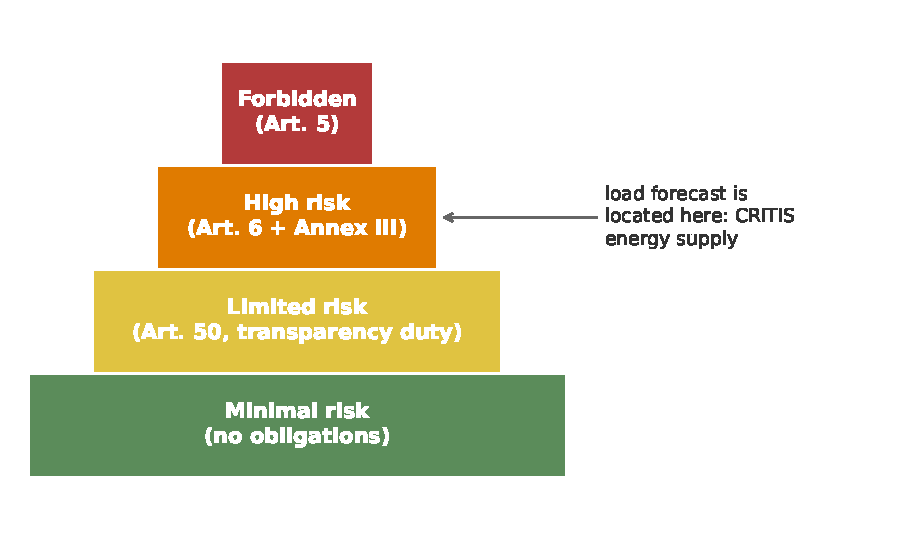
\includegraphics[keepaspectratio]{index_files/figure-pdf/fig-risk-pyramid-output-1.pdf}}

}

\caption{\label{fig-risk-pyramid}Risk pyramid of the AI Act. The top
(forbidden) is very narrow --- only a handful of applications are
inadmissible under Art. 5. The base (minimal risk) is wide --- the vast
majority of AI systems fall into the lowest tier and have no
obligations. The load forecast covered by this course falls into the
second tier (high-risk) under Annex III No.~2 of the AI Act (management
and operation of critical infrastructure).}

\end{figure}%

The use case of this course --- electric load forecasting for a grid
operator --- clearly lies in the second tier (high risk), because Annex
III No.~2 of the AI Act explicitly lists systems for the management of
critical infrastructure. The following chapters show how the obligations
from Art. 9 to 15 of the AI Act can be fulfilled \emph{technically} ---
not via additional prose documents, but via code that guarantees
specific properties.

\section*{The four code rules (CR-1 to CR-4)}\label{sec-cr}
\addcontentsline{toc}{section}{The four code rules (CR-1 to CR-4)}

\markright{The four code rules (CR-1 to CR-4)}

\texttt{spotforecast2-safe} operationalises the regulatory requirements
through four non-negotiable code rules. They form the backbone of the
entire course; every one of the ten chapters refers to at least one of
them.

{\def\LTcaptype{none} % do not increment counter
\begin{longtable}[]{@{}
  >{\centering\arraybackslash}p{(\linewidth - 6\tabcolsep) * \real{0.0448}}
  >{\raggedright\arraybackslash}p{(\linewidth - 6\tabcolsep) * \real{0.1866}}
  >{\raggedright\arraybackslash}p{(\linewidth - 6\tabcolsep) * \real{0.6194}}
  >{\raggedright\arraybackslash}p{(\linewidth - 6\tabcolsep) * \real{0.1493}}@{}}
\toprule\noalign{}
\begin{minipage}[b]{\linewidth}\centering
Rule
\end{minipage} & \begin{minipage}[b]{\linewidth}\raggedright
Short form
\end{minipage} & \begin{minipage}[b]{\linewidth}\raggedright
What it is about
\end{minipage} & \begin{minipage}[b]{\linewidth}\raggedright
AI Act link
\end{minipage} \\
\midrule\noalign{}
\endhead
\bottomrule\noalign{}
\endlastfoot
CR-1 & No dead code & Every function, class, branch is reached by a test
or docstring example. & Art. 9, 13 \\
CR-2 & Determinism & Same input, bit-identical output. Fixed seeds,
fixed iteration order. & Art. 12, 15 \\
CR-3 & Fail-safe processing & Invalid inputs (NaN, wrong dtype) raise an
\emph{explicit} exception instead of being silently imputed. & Art. 10,
15 \\
CR-4 & Minimal CVE attack surface & A short, versioned deny-list of
forbidden dependencies, enforced by a test against the lockfile. & Art.
15 \\
\end{longtable}
}

The detailed wording of the rules and their connection to the IEC
62443-4-1 norm can be found in the package's companion report under
\emph{Design principles}. For this course the rules of thumb suffice:

\begin{itemize}
\tightlist
\item
  \emph{CR-1} ensures that every line of code that ever runs has also
  been checked at some point.
\item
  \emph{CR-2} ensures that you can reproduce a result, even if you
  repeat it a year later.
\item
  \emph{CR-3} ensures that the system never silently guesses but always
  asks back when something is missing.
\item
  \emph{CR-4} ensures that the list of libraries your system depends on
  stays small --- because each dependency is a potential entry point for
  security vulnerabilities.
\end{itemize}

In the ten chapters that follow, you will see how these rules translate
into concrete safeguards --- at the very moment when
\texttt{spotforecast2-safe} does something that another library would
just wave through.

\section*{Roadmap through the
chapters}\label{roadmap-through-the-chapters}
\addcontentsline{toc}{section}{Roadmap through the chapters}

\markright{Roadmap through the chapters}

The lecture notes follow the order of the running example ``electric
load forecasting'': a complete load-forecasting pipeline for an ENTSO-E
market zone, from data acquisition to reproducibility audit.

{\def\LTcaptype{none} % do not increment counter
\begin{longtable}[]{@{}
  >{\centering\arraybackslash}p{(\linewidth - 6\tabcolsep) * \real{0.0978}}
  >{\raggedright\arraybackslash}p{(\linewidth - 6\tabcolsep) * \real{0.5870}}
  >{\raggedright\arraybackslash}p{(\linewidth - 6\tabcolsep) * \real{0.1957}}
  >{\raggedright\arraybackslash}p{(\linewidth - 6\tabcolsep) * \real{0.1196}}@{}}
\toprule\noalign{}
\begin{minipage}[b]{\linewidth}\centering
Chapter
\end{minipage} & \begin{minipage}[b]{\linewidth}\raggedright
Content
\end{minipage} & \begin{minipage}[b]{\linewidth}\raggedright
Code rule
\end{minipage} & \begin{minipage}[b]{\linewidth}\raggedright
AI Act
\end{minipage} \\
\midrule\noalign{}
\endhead
\bottomrule\noalign{}
\endlastfoot
01 & Switch on the audit log & CR-1 & Art. 12 \\
02 & Load live data from ENTSO-E & CR-2 & Art. 10 \\
03 & Annotate data anomalies explicitly & \textbf{CR-3} & Art. 10 \\
04 & Handle data gaps explicitly & \textbf{CR-3} & Art. 10 \\
05 & Separate training and evaluation range & CR-2 & Art. 10 \\
06 & Calendar features + real weather data & CR-3 & Art. 10 \\
07 & Instantiate and train the forecaster & CR-2, \textbf{CR-4} & Art.
9, 15 \\
08 & Produce a 24-hour forecast & CR-1 & Art. 13 \\
09 & Measure accuracy (MAE, RMSE, MAPE) & CR-2, CR-3 & \textbf{Art.
15} \\
10 & Rolling-origin backtest & CR-2 & Art. 9 \\
11 & Provenance and reproducibility & CR-1 to CR-4 & Art. 11, 12 \\
12 & Live challenge: forecasting energy consumption & CR-1 to CR-4 &
Art. 10, 12, 13, 15 \\
\end{longtable}
}

\section*{How to read these notes with
Claude}\label{how-to-read-these-notes-with-claude}
\addcontentsline{toc}{section}{How to read these notes with Claude}

\markright{How to read these notes with Claude}

Every chapter ends with an \emph{Exercises} box. The exercises are
phrased so that you can paste them directly into the AI assistant Claude
(e.g.~\url{https://claude.ai} or \emph{Claude Code} in the terminal) to
explore the source code of \texttt{spotforecast2-safe} on your own.

A typical exercise looks like this:

\begin{quote}
\emph{Ask Claude:} ``Show me the source code of
\texttt{spotforecast2\_safe.preprocessing.LinearlyInterpolateTS}.
Explain line by line how the \texttt{on\_missing} parameter changes the
behaviour. Write a Python example that compares all three permitted
values (`raise', `ffill\_bfill', `passthrough') on the same data
snippet.''
\end{quote}

We recommend really putting each exercise to Claude rather than googling
the answer yourself. The learning effect comes from the dialogue in
which you question Claude's explanation, push back on an insufficient
answer, ask for a concrete example, or probe for the connection to the
AI Act or to one of the four code rules.

\section*{Preparing your environment}\label{preparing-your-environment}
\addcontentsline{toc}{section}{Preparing your environment}

\markright{Preparing your environment}

For the live-data chapters (02, 06) you need two things:

\begin{itemize}
\item
  A free \emph{ENTSO-E Restful API} key. You can request it at
  \url{https://transparency.entsoe.eu/} after registering with a
  professional email address. Export it in your shell before rendering:

\begin{Shaded}
\begin{Highlighting}[]
\BuiltInTok{export} \VariableTok{ENTSOE\_API\_KEY}\OperatorTok{=}\StringTok{"your{-}token{-}here"}
\end{Highlighting}
\end{Shaded}
\item
  An active internet connection for Open-Meteo. Open-Meteo requires no
  key for the archive or forecast API.
\end{itemize}

The render command is:

\begin{Shaded}
\begin{Highlighting}[]
\BuiltInTok{cd}\NormalTok{ lecture}
\VariableTok{QUARTO\_PYTHON}\OperatorTok{=}\VariableTok{$HOME}\NormalTok{/workspace/Lehre.d/ddmo{-}sose{-}26/.venv/bin/python3 }\ExtensionTok{quarto}\NormalTok{ render}
\end{Highlighting}
\end{Shaded}

When you run this command a second time, the once-fetched ENTSO-E and
weather data are served from \texttt{\_freeze/} and \texttt{\_cache/}; a
re-render then takes under thirty seconds. Any change to a chapter's
source invalidates only that chapter's cache.

\protect\phantomsection\label{chk-env}
\begin{Shaded}
\begin{Highlighting}[]
\ImportTok{import}\NormalTok{ os}

\ControlFlowTok{if} \StringTok{"ENTSOE\_API\_KEY"} \KeywordTok{not} \KeywordTok{in}\NormalTok{ os.environ:}
    \ControlFlowTok{raise} \PreprocessorTok{RuntimeError}\NormalTok{(}
        \StringTok{"Set ENTSOE\_API\_KEY in the shell before rendering chapter 02. "}
        \StringTok{"Request a key at: https://transparency.entsoe.eu/"}
\NormalTok{    )}
\BuiltInTok{print}\NormalTok{(}\StringTok{"Environment looks good. You can now run \textasciigrave{}quarto render\textasciigrave{}."}\NormalTok{)}
\end{Highlighting}
\end{Shaded}

\begin{tcolorbox}[enhanced jigsaw, arc=.35mm, bottomrule=.15mm, bottomtitle=1mm, breakable, colback=white, colbacktitle=quarto-callout-note-color!10!white, colframe=quarto-callout-note-color-frame, coltitle=black, left=2mm, leftrule=.75mm, opacityback=0, opacitybacktitle=0.6, rightrule=.15mm, title=\textcolor{quarto-callout-note-color}{\faInfo}\hspace{0.5em}{Determinism despite live data}, titlerule=0mm, toprule=.15mm, toptitle=1mm]

Live APIs return time-dependent values. So that our pipeline can still
satisfy the CR-2 condition of bit-identical reproducibility, we pin the
endpoints of the time window under consideration in a single constant
that is passed to all chapters:

\begin{Shaded}
\begin{Highlighting}[]
\NormalTok{DATA\_START }\OperatorTok{=} \StringTok{"2024{-}01{-}01 00:00+00:00"}
\NormalTok{DATA\_END   }\OperatorTok{=} \StringTok{"2024{-}12{-}31 23:00+00:00"}
\NormalTok{COUNTRY    }\OperatorTok{=} \StringTok{"DE"}
\end{Highlighting}
\end{Shaded}

That way all students get identical data for an identical time window.

\end{tcolorbox}

\bookmarksetup{startatroot}

\chapter{Switch on the audit log}\label{sec-audit}

\begin{tcolorbox}[enhanced jigsaw, arc=.35mm, bottomrule=.15mm, bottomtitle=1mm, breakable, colback=white, colbacktitle=quarto-callout-note-color!10!white, colframe=quarto-callout-note-color-frame, coltitle=black, left=2mm, leftrule=.75mm, opacityback=0, opacitybacktitle=0.6, rightrule=.15mm, title=\textcolor{quarto-callout-note-color}{\faInfo}\hspace{0.5em}{Learning objective}, titlerule=0mm, toprule=.15mm, toptitle=1mm]

You can explain \emph{why} a safety-critical library has to keep a
record of what it does from the very first line of code on, and you can
switch on \texttt{spotforecast2-safe}'s audit log with two lines of
code.

\end{tcolorbox}

\section{Why log at all?}\label{why-log-at-all}

Imagine that the load-forecasting system from the introduction really
did predict 65 instead of 72 gigawatts at 08:00, and the grid is
therefore severely under-supplied. The supervisory authority asks:
\emph{Which data were available to the model at 06:00, with which
hyperparameters was it trained, which version of the library was running
in production?} If the answers are not in a verifiable log, the incident
is considered unreconstructable --- and the operator has breached their
duty under Art. 12 of the AI Act (\emph{record-keeping}).

\texttt{spotforecast2-safe} therefore writes every action ---
initialisation of the forecaster, data download, training run,
prediction --- into a structured log. We switch this log on
\emph{first}, before doing anything else, because the initialisation
itself is already a log-worthy action. This practice instantiates both
Art. 12 of the AI Act and the discipline of a structured audit log
anchored in process rule PR-4. It connects directly to code rule
\textbf{CR-1} (no dead code): every function that is logged \emph{has},
by definition, been executed, hence is not dead.

\section{Code in action}\label{code-in-action}

\protect\phantomsection\label{setup-logger}
\begin{Shaded}
\begin{Highlighting}[]
\ImportTok{import}\NormalTok{ logging}
\ImportTok{from}\NormalTok{ pathlib }\ImportTok{import}\NormalTok{ Path}
\ImportTok{from}\NormalTok{ spotforecast2\_safe.manager.logger }\ImportTok{import}\NormalTok{ setup\_logging}

\CommentTok{\# We write into a project{-}local log directory:}
\NormalTok{log\_dir }\OperatorTok{=}\NormalTok{ Path(}\StringTok{"\_cache/logs"}\NormalTok{)}
\NormalTok{log\_dir.mkdir(parents}\OperatorTok{=}\VariableTok{True}\NormalTok{, exist\_ok}\OperatorTok{=}\VariableTok{True}\NormalTok{)}

\NormalTok{logger, log\_path }\OperatorTok{=}\NormalTok{ setup\_logging(level}\OperatorTok{=}\NormalTok{logging.INFO, log\_dir}\OperatorTok{=}\NormalTok{log\_dir)}
\NormalTok{logger.info(}\StringTok{"Course run starts: load{-}forecasting pipeline (chapter 01)."}\NormalTok{)}
\BuiltInTok{print}\NormalTok{(}\SpecialStringTok{f"Log file: }\SpecialCharTok{\{}\NormalTok{log\_path}\SpecialCharTok{.}\NormalTok{name }\ControlFlowTok{if}\NormalTok{ log\_path }\ControlFlowTok{else} \StringTok{\textquotesingle{}\textless{}stdout only\textgreater{}\textquotesingle{}}\SpecialCharTok{\}}\SpecialStringTok{"}\NormalTok{)}
\end{Highlighting}
\end{Shaded}

\begin{verbatim}
2026-05-31 21:50:57,585 - task_safe_n_to_1 - INFO - Persistent logging initialized at: _cache/logs/task_safe_n_to_1_20260531_215057.log
2026-05-31 21:50:57,586 - task_safe_n_to_1 - INFO - Course run starts: load-forecasting pipeline (chapter 01).
Log file: task_safe_n_to_1_20260531_215057.log
\end{verbatim}

The call returns two things: a \texttt{logger}, with which we record
every relevant action from now on, and a \texttt{log\_path} pointing to
the concrete file where the log lives. The default logger name is
\texttt{task\_safe\_n\_to\_1}. From now on every function in
\texttt{spotforecast2-safe} that logs its own steps writes into the same
file --- without us having to forward where logging happens.

\section{What is inside the log
file?}\label{what-is-inside-the-log-file}

\protect\phantomsection\label{log-content}
\begin{Shaded}
\begin{Highlighting}[]
\ControlFlowTok{if}\NormalTok{ log\_path }\KeywordTok{is} \KeywordTok{not} \VariableTok{None} \KeywordTok{and}\NormalTok{ log\_path.exists():}
    \BuiltInTok{print}\NormalTok{(}\StringTok{"{-}{-}{-} first line of the log {-}{-}{-}"}\NormalTok{)}
    \BuiltInTok{print}\NormalTok{(log\_path.read\_text().splitlines()[}\DecValTok{0}\NormalTok{])}
\ControlFlowTok{else}\NormalTok{:}
    \BuiltInTok{print}\NormalTok{(}\StringTok{"No file handler active; the log only goes to stdout."}\NormalTok{)}
\end{Highlighting}
\end{Shaded}

\begin{verbatim}
--- first line of the log ---
{"schema_version":"1.0.0","timestamp_utc":"2026-05-31T19:50:57.585840Z","logger":"task_safe_n_to_1","level":"INFO","event":"audit_log_init","message":"Persistent logging initialized at: _cache/logs/task_safe_n_to_1_20260531_215057.log"}
\end{verbatim}

Every entry contains timestamp, logger name, level
(INFO/WARNING/ERROR/DEBUG) and text. These four fields are enough for a
later auditor to reconstruct the exact order and content of every
action.

\section{Visualisation: How an audit run
unfolds}\label{visualisation-how-an-audit-run-unfolds}

The following sequence flow shows which actors talk to each other while
the pipeline renders. You will fill it out step by step in the coming
chapters --- each chapter adds a new arrow.

\begin{Shaded}
\begin{Highlighting}[]
\NormalTok{sequenceDiagram}
\NormalTok{    participant Student}
\NormalTok{    participant Pipeline as Pipeline (Quarto)}
\NormalTok{    participant Logger}
\NormalTok{    participant File as Log file}

\NormalTok{    Student{-}\textgreater{}\textgreater{}Pipeline: quarto render}
\NormalTok{    Pipeline{-}\textgreater{}\textgreater{}Logger: setup\_logging()}
\NormalTok{    Logger{-}\textgreater{}\textgreater{}File: open, write header}
\NormalTok{    Pipeline{-}\textgreater{}\textgreater{}Logger: info("run starts")}
\NormalTok{    Logger{-}\textgreater{}\textgreater{}File: append line with timestamp}
\NormalTok{    Note over File: later auditor reads here}
\end{Highlighting}
\end{Shaded}

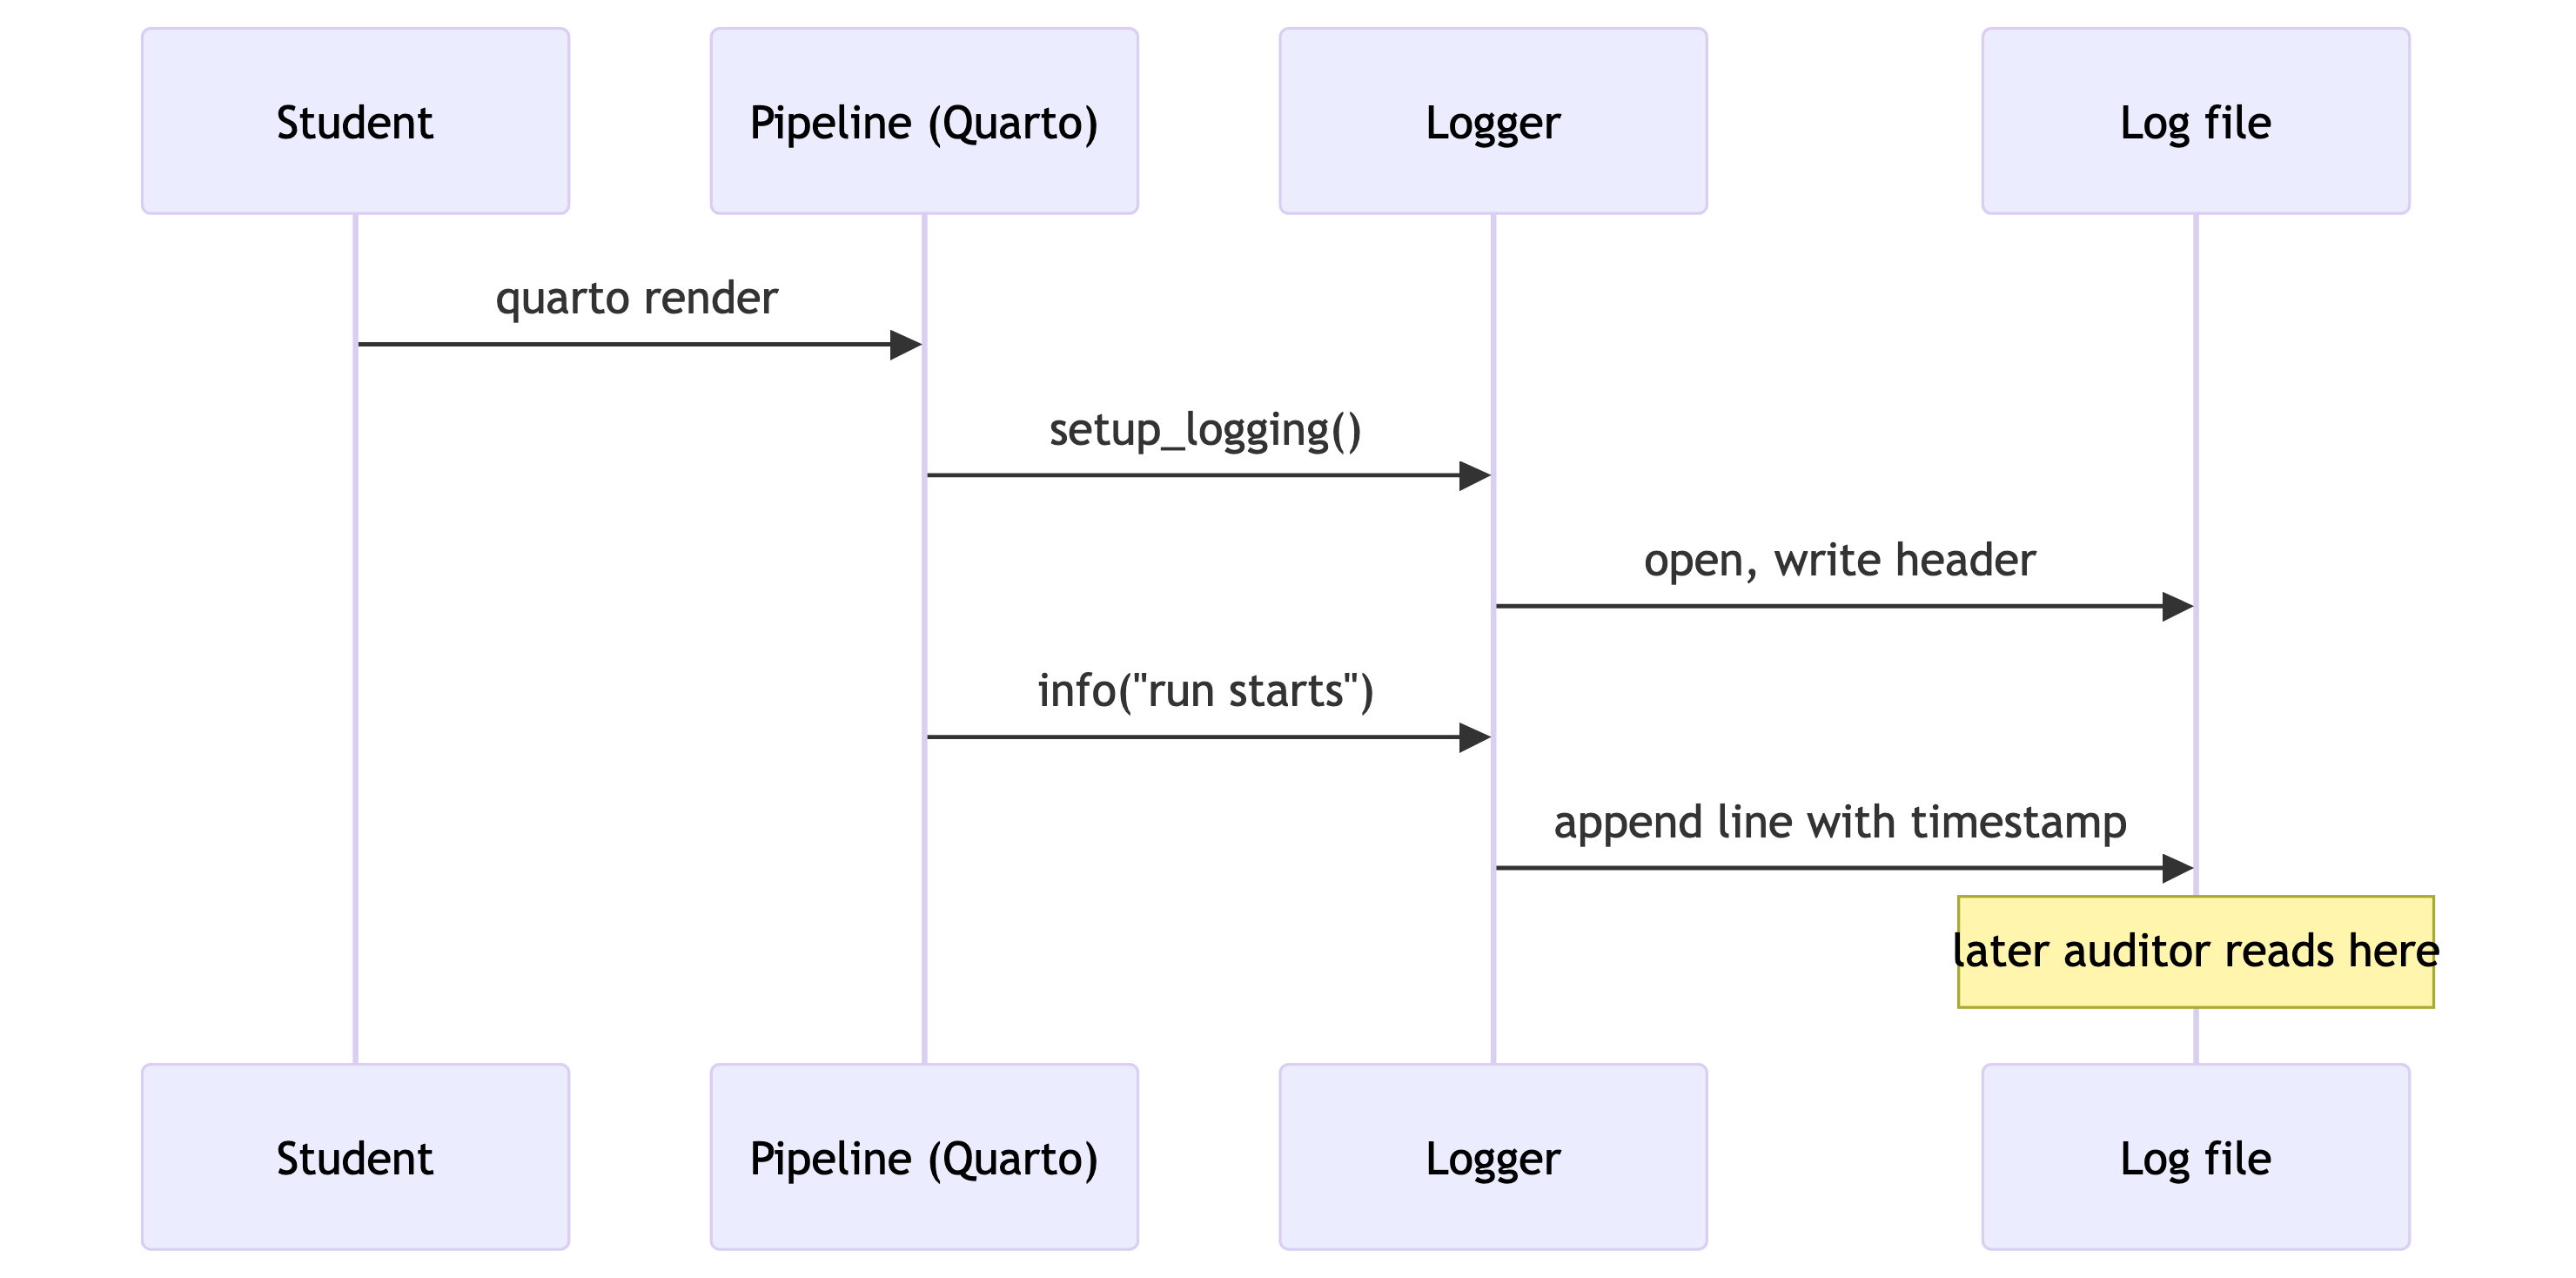
\includegraphics[width=9.43in,height=4.69in]{01_audit_log_files/figure-latex/mermaid-figure-1.png}

\begin{tcolorbox}[enhanced jigsaw, arc=.35mm, bottomrule=.15mm, bottomtitle=1mm, breakable, colback=white, colbacktitle=quarto-callout-tip-color!10!white, colframe=quarto-callout-tip-color-frame, coltitle=black, left=2mm, leftrule=.75mm, opacityback=0, opacitybacktitle=0.6, rightrule=.15mm, title=\textcolor{quarto-callout-tip-color}{\faLightbulb}\hspace{0.5em}{Exercises (with Claude)}, titlerule=0mm, toprule=.15mm, toptitle=1mm]

\begin{enumerate}
\def\labelenumi{\arabic{enumi}.}
\tightlist
\item
  \emph{Source-code exploration.} Ask Claude to display the source of
  \texttt{spotforecast2\_safe.manager.logger.setup\_logging} and to
  explain how the function makes sure that file creation does \emph{not}
  abort the entire run when the directory is read-only. Which code rule
  addresses this behaviour?
\item
  \emph{Comparison with \texttt{print}.} Discuss with Claude why
  \texttt{print()} would be \emph{unsuitable} for an audit log. At least
  three traceable reasons should be given, each tied to Art. 12 of the
  AI Act or to one of the four code rules.
\item
  \emph{Advanced exercise.} Have Claude write a mini pipeline that
  performs two training runs with different seeds and, from the audit
  log alone, figures out in which order the runs took place. Explain why
  exactly this information is decisive for a later reproduction.
\end{enumerate}

\end{tcolorbox}

\bookmarksetup{startatroot}

\chapter{Loading live data from ENTSO-E}\label{sec-entsoe}

\begin{tcolorbox}[enhanced jigsaw, arc=.35mm, bottomrule=.15mm, bottomtitle=1mm, breakable, colback=white, colbacktitle=quarto-callout-note-color!10!white, colframe=quarto-callout-note-color-frame, coltitle=black, left=2mm, leftrule=.75mm, opacityback=0, opacitybacktitle=0.6, rightrule=.15mm, title=\textcolor{quarto-callout-note-color}{\faInfo}\hspace{0.5em}{Learning objective}, titlerule=0mm, toprule=.15mm, toptitle=1mm]

You can use the function \texttt{download\_new\_data} from
\texttt{spotforecast2\_safe.downloader} to drop a real electric-load
time series for an ENTSO-E market zone into a local CSV, and you can
explain how this function guarantees CR-2 (determinism) despite the live
API call.

\end{tcolorbox}

\section{What the running example in the report was
about}\label{what-the-running-example-in-the-report-was-about}

The running example in the companion report generates a \emph{synthetic}
load series, because the document must render deterministically and
offline. For a course that wants to teach real engineering practice, we
replace the synthetic series with real data from the \emph{ENTSO-E
Transparency Platform} --- the central database of the European Network
of Transmission System Operators for Electricity. ENTSO-E publishes
hourly the actual and forecast load for every market zone in Europe.

\section{AI Act link}\label{ai-act-link}

Data origin is a central concern of the AI Act: Art. 10(2) obliges
providers and deployers to maintain \emph{data management and data
governance procedures} which, among other things, document origin,
collection method and assumptions about data processing. By pulling the
data directly from the ENTSO-E API rather than from a spreadsheet of
unknown origin, we keep the provenance explicit and documentable.

Code rule \textbf{CR-2} (determinism) would be jeopardised by a live
API, because the API returns different values tomorrow than today. We
solve this by pinning the date \emph{window}: all students load exactly
the same period (\texttt{DATA\_START} to \texttt{DATA\_END}), therefore
receive byte-identical values, and can compare their results with each
other.

\section{Code in action}\label{code-in-action-1}

\protect\phantomsection\label{env-prep}
\begin{Shaded}
\begin{Highlighting}[]
\ImportTok{import}\NormalTok{ os}
\ImportTok{from}\NormalTok{ pathlib }\ImportTok{import}\NormalTok{ Path}

\CommentTok{\# Keep cache directory local to the book rather than in the student\textquotesingle{}s home:}
\NormalTok{DATA\_HOME }\OperatorTok{=}\NormalTok{ Path(}\VariableTok{\_\_file\_\_}\NormalTok{).parent.resolve() }\OperatorTok{/} \StringTok{"\_cache"} \OperatorTok{/} \StringTok{"spotforecast2\_data"} \OperatorTok{\textbackslash{}}
    \ControlFlowTok{if} \StringTok{"\_\_file\_\_"} \KeywordTok{in} \BuiltInTok{dir}\NormalTok{() }\ControlFlowTok{else}\NormalTok{ Path.cwd() }\OperatorTok{/} \StringTok{"\_cache"} \OperatorTok{/} \StringTok{"spotforecast2\_data"}
\NormalTok{DATA\_HOME.mkdir(parents}\OperatorTok{=}\VariableTok{True}\NormalTok{, exist\_ok}\OperatorTok{=}\VariableTok{True}\NormalTok{)}
\NormalTok{os.environ[}\StringTok{"SPOTFORECAST2\_DATA"}\NormalTok{] }\OperatorTok{=} \BuiltInTok{str}\NormalTok{(DATA\_HOME)}

\CommentTok{\# Fixed constants: the same window for every student}
\NormalTok{DATA\_START }\OperatorTok{=} \StringTok{"202401010000"}   \CommentTok{\# 2024{-}01{-}01 00:00 UTC}
\NormalTok{DATA\_END   }\OperatorTok{=} \StringTok{"202412312300"}   \CommentTok{\# 2024{-}12{-}31 23:00 UTC}
\NormalTok{COUNTRY    }\OperatorTok{=} \StringTok{"DE"}             \CommentTok{\# ENTSO{-}E country code: Germany{-}Luxembourg market zone}

\BuiltInTok{print}\NormalTok{(}\SpecialStringTok{f"Data home: }\SpecialCharTok{\{}\NormalTok{DATA\_HOME}\SpecialCharTok{\}}\SpecialStringTok{"}\NormalTok{)}
\BuiltInTok{print}\NormalTok{(}\SpecialStringTok{f"Window:    }\SpecialCharTok{\{}\NormalTok{DATA\_START}\SpecialCharTok{\}}\SpecialStringTok{ to }\SpecialCharTok{\{}\NormalTok{DATA\_END}\SpecialCharTok{\}}\SpecialStringTok{"}\NormalTok{)}
\BuiltInTok{print}\NormalTok{(}\SpecialStringTok{f"Country:   }\SpecialCharTok{\{}\NormalTok{COUNTRY}\SpecialCharTok{\}}\SpecialStringTok{"}\NormalTok{)}
\end{Highlighting}
\end{Shaded}

\begin{verbatim}
Data home: /Users/bartz/workspace/Lehre.d/ddmo-sose-26/lecture/_cache/spotforecast2_data
Window:    202401010000 to 202412312300
Country:   DE
\end{verbatim}

\protect\phantomsection\label{download-entsoe}
\begin{Shaded}
\begin{Highlighting}[]
\ImportTok{import}\NormalTok{ logging}
\ImportTok{from}\NormalTok{ spotforecast2\_safe.downloader.entsoe }\ImportTok{import}\NormalTok{ download\_new\_data}
\ImportTok{from}\NormalTok{ spotforecast2\_safe.data.fetch\_data }\ImportTok{import}\NormalTok{ fetch\_data, get\_data\_home}

\NormalTok{logging.getLogger(}\StringTok{"spotforecast2\_safe.downloader.entsoe"}\NormalTok{).setLevel(logging.INFO)}

\NormalTok{interim }\OperatorTok{=}\NormalTok{ get\_data\_home() }\OperatorTok{/} \StringTok{"interim"} \OperatorTok{/} \StringTok{"energy\_load.csv"}

\ControlFlowTok{if}\NormalTok{ interim.exists():}
    \BuiltInTok{print}\NormalTok{(}\SpecialStringTok{f"Cache hit, no download needed: }\SpecialCharTok{\{}\NormalTok{interim}\SpecialCharTok{.}\NormalTok{relative\_to(DATA\_HOME)}\SpecialCharTok{\}}\SpecialStringTok{"}\NormalTok{)}
\ControlFlowTok{else}\NormalTok{:}
\NormalTok{    api\_key }\OperatorTok{=}\NormalTok{ os.environ.get(}\StringTok{"ENTSOE\_API\_KEY"}\NormalTok{)}
    \ControlFlowTok{if} \KeywordTok{not}\NormalTok{ api\_key:}
        \ControlFlowTok{raise} \PreprocessorTok{RuntimeError}\NormalTok{(}
            \StringTok{"ENTSOE\_API\_KEY is not set. Register for free at "}
            \StringTok{"https://transparency.entsoe.eu/, obtain a token and export "}
            \StringTok{"it before rendering: export ENTSOE\_API\_KEY=..."}\NormalTok{)}
\NormalTok{    download\_new\_data(}
\NormalTok{        api\_key}\OperatorTok{=}\NormalTok{api\_key,}
\NormalTok{        country\_code}\OperatorTok{=}\NormalTok{COUNTRY,}
\NormalTok{        start}\OperatorTok{=}\NormalTok{DATA\_START,}
\NormalTok{        end}\OperatorTok{=}\NormalTok{DATA\_END,}
\NormalTok{        force}\OperatorTok{=}\VariableTok{True}\NormalTok{,}
\NormalTok{    )}
    \BuiltInTok{print}\NormalTok{(}\SpecialStringTok{f"Download complete, stored at }\SpecialCharTok{\{}\NormalTok{interim}\SpecialCharTok{.}\NormalTok{relative\_to(DATA\_HOME)}\SpecialCharTok{\}}\SpecialStringTok{"}\NormalTok{)}
\end{Highlighting}
\end{Shaded}

\begin{verbatim}
Cache hit, no download needed: interim/energy_load.csv
\end{verbatim}

After the download the merged CSV file lives at
\texttt{\_cache/spotforecast2\_data/interim/energy\_load.csv}. On the
next render of this chapter the block skips the download because the
file already exists --- and Quarto serves the pre-computed result from
\texttt{\_freeze/}.

\section{Reading and checking the
data}\label{reading-and-checking-the-data}

\protect\phantomsection\label{load-and-check}
\begin{Shaded}
\begin{Highlighting}[]
\ImportTok{import}\NormalTok{ pandas }\ImportTok{as}\NormalTok{ pd}

\NormalTok{df }\OperatorTok{=}\NormalTok{ fetch\_data(filename}\OperatorTok{=}\BuiltInTok{str}\NormalTok{(interim))}
\NormalTok{df.index }\OperatorTok{=}\NormalTok{ pd.to\_datetime(df.index, utc}\OperatorTok{=}\VariableTok{True}\NormalTok{)}

\CommentTok{\# We focus on the "Actual Load" column:}
\NormalTok{load\_col }\OperatorTok{=} \BuiltInTok{next}\NormalTok{(c }\ControlFlowTok{for}\NormalTok{ c }\KeywordTok{in}\NormalTok{ df.columns }\ControlFlowTok{if} \StringTok{"Actual"} \KeywordTok{in}\NormalTok{ c }\KeywordTok{and} \StringTok{"Load"} \KeywordTok{in}\NormalTok{ c)}
\NormalTok{y }\OperatorTok{=}\NormalTok{ df[load\_col].astype(}\BuiltInTok{float}\NormalTok{).rename(}\StringTok{"load"}\NormalTok{)}

\CommentTok{\# ENTSO{-}E delivers 15{-}minute values for Germany; we aggregate to hourly}
\CommentTok{\# means so that the index matches our hourly weather series and the}
\CommentTok{\# hourly{-}lag logic of the forecaster.}
\ControlFlowTok{if}\NormalTok{ y.index.inferred\_freq }\OperatorTok{!=} \StringTok{"h"}\NormalTok{:}
\NormalTok{    y }\OperatorTok{=}\NormalTok{ y.resample(}\StringTok{"h"}\NormalTok{).mean()}

\BuiltInTok{print}\NormalTok{(}\SpecialStringTok{f"Columns in the file: }\SpecialCharTok{\{}\BuiltInTok{list}\NormalTok{(df.columns)}\SpecialCharTok{\}}\SpecialStringTok{"}\NormalTok{)}
\BuiltInTok{print}\NormalTok{(}\SpecialStringTok{f"Used column:         \textquotesingle{}}\SpecialCharTok{\{}\NormalTok{load\_col}\SpecialCharTok{\}}\SpecialStringTok{\textquotesingle{}"}\NormalTok{)}
\BuiltInTok{print}\NormalTok{(}\SpecialStringTok{f"Number of timestamps: }\SpecialCharTok{\{}\BuiltInTok{len}\NormalTok{(y)}\SpecialCharTok{:,\}}\SpecialStringTok{"}\NormalTok{)}
\BuiltInTok{print}\NormalTok{(}\SpecialStringTok{f"Time window:          }\SpecialCharTok{\{}\NormalTok{y}\SpecialCharTok{.}\NormalTok{index}\SpecialCharTok{.}\BuiltInTok{min}\NormalTok{()}\SpecialCharTok{\}}\SpecialStringTok{  ...  }\SpecialCharTok{\{}\NormalTok{y}\SpecialCharTok{.}\NormalTok{index}\SpecialCharTok{.}\BuiltInTok{max}\NormalTok{()}\SpecialCharTok{\}}\SpecialStringTok{"}\NormalTok{)}
\BuiltInTok{print}\NormalTok{(}\SpecialStringTok{f"Missing values:       }\SpecialCharTok{\{}\BuiltInTok{int}\NormalTok{(y.isna().}\BuiltInTok{sum}\NormalTok{())}\SpecialCharTok{\}}\SpecialStringTok{"}\NormalTok{)}
\end{Highlighting}
\end{Shaded}

\begin{verbatim}
Columns in the file: ['Forecasted Load', 'Actual Load']
Used column:         'Actual Load'
Number of timestamps: 8,783
Time window:          2024-01-01 00:00:00+00:00  ...  2024-12-31 22:00:00+00:00
Missing values:       0
\end{verbatim}

\section{Visualisation: one year of German
load}\label{visualisation-one-year-of-german-load}

\begin{Shaded}
\begin{Highlighting}[]
\ImportTok{import}\NormalTok{ matplotlib.pyplot }\ImportTok{as}\NormalTok{ plt}
\ImportTok{import}\NormalTok{ matplotlib.dates }\ImportTok{as}\NormalTok{ mdates}

\NormalTok{fig, ax }\OperatorTok{=}\NormalTok{ plt.subplots(figsize}\OperatorTok{=}\NormalTok{(}\FloatTok{8.5}\NormalTok{, }\FloatTok{3.5}\NormalTok{))}
\NormalTok{ax.plot(y.index, y.values }\OperatorTok{/} \DecValTok{1000}\NormalTok{, color}\OperatorTok{=}\StringTok{"\#1F4E79"}\NormalTok{, linewidth}\OperatorTok{=}\FloatTok{0.5}\NormalTok{)}
\NormalTok{ax.set\_ylabel(}\StringTok{"Load [GW]"}\NormalTok{)}
\NormalTok{ax.set\_xlabel(}\StringTok{"Time"}\NormalTok{)}
\NormalTok{ax.set\_title(}\SpecialStringTok{f"ENTSO{-}E market zone }\SpecialCharTok{\{}\NormalTok{COUNTRY}\SpecialCharTok{\}}\SpecialStringTok{: 2024"}\NormalTok{)}
\NormalTok{ax.grid(}\VariableTok{True}\NormalTok{, color}\OperatorTok{=}\StringTok{"\#E5E5E5"}\NormalTok{, linewidth}\OperatorTok{=}\FloatTok{0.5}\NormalTok{)}
\NormalTok{ax.xaxis.set\_major\_locator(mdates.MonthLocator())}
\NormalTok{ax.xaxis.set\_major\_formatter(mdates.DateFormatter(}\StringTok{"\%b"}\NormalTok{))}
\ControlFlowTok{for}\NormalTok{ s }\KeywordTok{in}\NormalTok{ (}\StringTok{"top"}\NormalTok{, }\StringTok{"right"}\NormalTok{):}
\NormalTok{    ax.spines[s].set\_visible(}\VariableTok{False}\NormalTok{)}
\NormalTok{fig.tight\_layout()}
\NormalTok{plt.show()}
\end{Highlighting}
\end{Shaded}

\begin{figure}[H]

\centering{

\pandocbounded{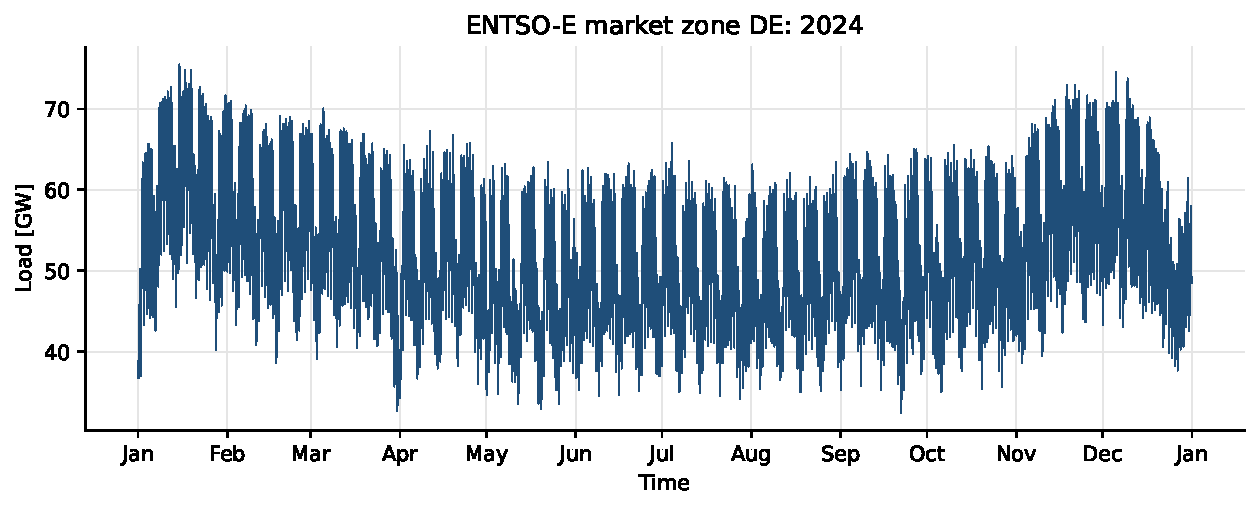
\includegraphics[keepaspectratio]{02_entsoe_data_files/figure-pdf/fig-entsoe-overview-output-1.pdf}}

}

\caption{\label{fig-entsoe-overview}Actual electric load of the
Germany-Luxembourg market zone over the year 2024, quarter-hourly
resolution (aggregated by ENTSO-E to hourly). The daily and weekly
rhythm is clearly visible, as well as the seasonal reduction during
summer weeks and holidays.}

\end{figure}%

\begin{Shaded}
\begin{Highlighting}[]
\NormalTok{week }\OperatorTok{=}\NormalTok{ y.loc[}\StringTok{"2024{-}02{-}05"}\NormalTok{:}\StringTok{"2024{-}02{-}12"}\NormalTok{]}

\NormalTok{fig, ax }\OperatorTok{=}\NormalTok{ plt.subplots(figsize}\OperatorTok{=}\NormalTok{(}\FloatTok{8.5}\NormalTok{, }\FloatTok{3.0}\NormalTok{))}
\NormalTok{ax.plot(week.index, week.values }\OperatorTok{/} \DecValTok{1000}\NormalTok{, color}\OperatorTok{=}\StringTok{"\#1F4E79"}\NormalTok{, linewidth}\OperatorTok{=}\FloatTok{1.0}\NormalTok{)}
\NormalTok{ax.set\_ylabel(}\StringTok{"Load [GW]"}\NormalTok{)}
\NormalTok{ax.grid(}\VariableTok{True}\NormalTok{, color}\OperatorTok{=}\StringTok{"\#E5E5E5"}\NormalTok{, linewidth}\OperatorTok{=}\FloatTok{0.5}\NormalTok{)}
\NormalTok{ax.xaxis.set\_major\_locator(mdates.DayLocator())}
\NormalTok{ax.xaxis.set\_major\_formatter(mdates.DateFormatter(}\StringTok{"\%a }\SpecialCharTok{\%{-}d}\StringTok{.\%{-}m"}\NormalTok{))}
\ControlFlowTok{for}\NormalTok{ s }\KeywordTok{in}\NormalTok{ (}\StringTok{"top"}\NormalTok{, }\StringTok{"right"}\NormalTok{):}
\NormalTok{    ax.spines[s].set\_visible(}\VariableTok{False}\NormalTok{)}
\NormalTok{fig.tight\_layout()}
\NormalTok{plt.show()}
\end{Highlighting}
\end{Shaded}

\begin{figure}[H]

\centering{

\pandocbounded{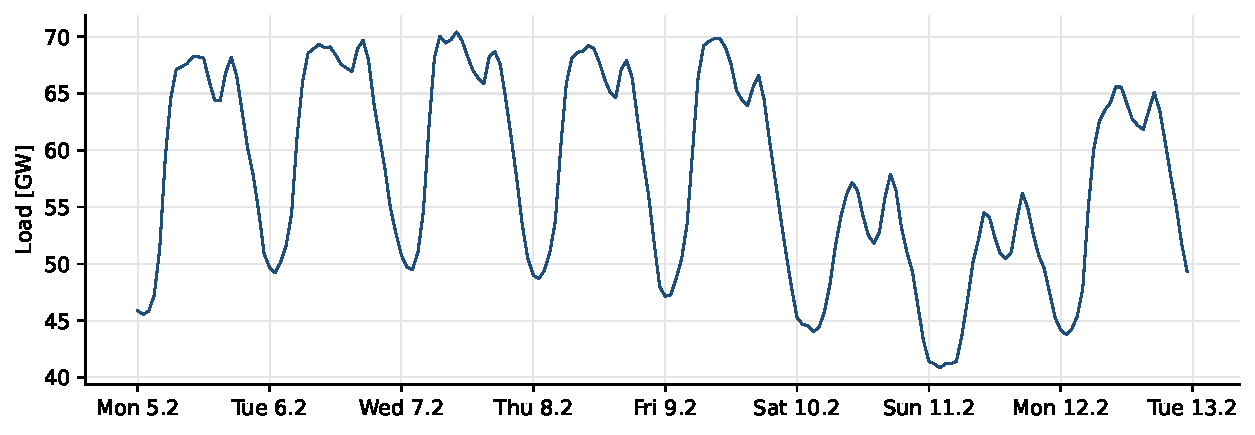
\includegraphics[keepaspectratio]{02_entsoe_data_files/figure-pdf/fig-entsoe-week-output-1.pdf}}

}

\caption{\label{fig-entsoe-week}A sample week in February 2024. The
weekly structure (weekday peak, weekend trough) and the typical
morning/evening double peak are immediately visible.}

\end{figure}%

\section{Persisting state}\label{persisting-state}

We make the series \texttt{y} available to the following chapters. In a
book the variables from one chapter are not automatically visible in the
next; we therefore save the loaded state in a small Parquet file which
the next chapters read back.

\protect\phantomsection\label{persist-load}
\begin{Shaded}
\begin{Highlighting}[]
\NormalTok{shared }\OperatorTok{=}\NormalTok{ Path(}\StringTok{"\_cache/shared"}\NormalTok{)}
\NormalTok{shared.mkdir(parents}\OperatorTok{=}\VariableTok{True}\NormalTok{, exist\_ok}\OperatorTok{=}\VariableTok{True}\NormalTok{)}
\NormalTok{y.to\_frame().to\_parquet(shared }\OperatorTok{/} \StringTok{"load\_de\_2024.parquet"}\NormalTok{)}
\BuiltInTok{print}\NormalTok{(}\SpecialStringTok{f"Load series persisted: }\SpecialCharTok{\{}\NormalTok{shared }\OperatorTok{/} \StringTok{\textquotesingle{}load\_de\_2024.parquet\textquotesingle{}}\SpecialCharTok{\}}\SpecialStringTok{"}\NormalTok{)}
\end{Highlighting}
\end{Shaded}

\begin{verbatim}
Load series persisted: _cache/shared/load_de_2024.parquet
\end{verbatim}

\begin{tcolorbox}[enhanced jigsaw, arc=.35mm, bottomrule=.15mm, bottomtitle=1mm, breakable, colback=white, colbacktitle=quarto-callout-tip-color!10!white, colframe=quarto-callout-tip-color-frame, coltitle=black, left=2mm, leftrule=.75mm, opacityback=0, opacitybacktitle=0.6, rightrule=.15mm, title=\textcolor{quarto-callout-tip-color}{\faLightbulb}\hspace{0.5em}{Exercises (with Claude)}, titlerule=0mm, toprule=.15mm, toptitle=1mm]

\begin{enumerate}
\def\labelenumi{\arabic{enumi}.}
\tightlist
\item
  \emph{Understanding the \texttt{force} parameter.} Have Claude explain
  the source of \texttt{download\_new\_data} line by line, with
  particular focus on the block that checks \texttt{force=False} and
  \texttt{hours\_diff\ \textless{}\ 24}. What happens when you call the
  function twice in quick succession with \texttt{force=False} after
  data are already on disk? Which code rule addresses this behaviour?
\item
  \emph{Switching the market zone.} Ask Claude to show an alternative
  variant of the pipeline that loads market zone \texttt{FR} (France)
  instead of \texttt{DE} and plots both series side by side over the
  same February window. Which structural differences in the load stand
  out?
\item
  \emph{Documenting data provenance.} Ask Claude which five fields a
  minimal data-provenance note under Art. 10 of the AI Act should
  contain. Have Claude generate a concrete example note for our run
  (source URL, fetch timestamp, market zone, time window, hash of the
  CSV).
\end{enumerate}

\end{tcolorbox}

\bookmarksetup{startatroot}

\chapter{Annotate data gaps instead of inventing
them}\label{sec-annotation}

\begin{tcolorbox}[enhanced jigsaw, arc=.35mm, bottomrule=.15mm, bottomtitle=1mm, breakable, colback=white, colbacktitle=quarto-callout-note-color!10!white, colframe=quarto-callout-note-color-frame, coltitle=black, left=2mm, leftrule=.75mm, opacityback=0, opacitybacktitle=0.6, rightrule=.15mm, title=\textcolor{quarto-callout-note-color}{\faInfo}\hspace{0.5em}{Learning objective}, titlerule=0mm, toprule=.15mm, toptitle=1mm]

You understand why a safety-critical library \textbf{annotates} broken
rows instead of interpolating them, and you can assemble the three
building blocks \texttt{mark\_outliers}, \texttt{get\_missing\_weights}
and \texttt{WeightFunction} into a preprocessing pipeline that complies
with the AI Act.

\end{tcolorbox}

\section{Why not simply interpolate?}\label{why-not-simply-interpolate}

Linear interpolation (see Chapter~\ref{sec-missing}) fills gaps with
\emph{invented} values. For yesterday's weather forecast that is
uncritical; in a high-risk application under Annex III of the AI Act ---
such as load forecasting for a transmission system operator --- it leads
to two structural problems:

\begin{enumerate}
\def\labelenumi{\arabic{enumi}.}
\tightlist
\item
  \textbf{Auditability disappears.} In retrospect an interpolated hour
  looks to the auditor exactly like a real measurement. But Art. 12 of
  the AI Act demands that \emph{every} data-related action remains
  discoverable in the audit log.
\item
  \textbf{The model learns phantom data.} A forecaster that takes the
  interpolated value as a training target optimises its loss against
  invented values as well. The expected value of the learned function is
  biased in favour of the imputer --- rather than in favour of reality.
\end{enumerate}

The \texttt{spotforecast2-safe} library therefore follows the
\emph{``annotate, don't invent''} pattern: broken rows are set to
\texttt{NaN}, filled in via forward/backward fill only far enough that
the lag operator does not crash, and assigned weight \textbf{0} in the
training loss. The model \emph{sees} the compromised rows, but they do
not pull the gradient.

\section{AI Act link}\label{ai-act-link-1}

{\def\LTcaptype{none} % do not increment counter
\begin{longtable}[]{@{}
  >{\raggedright\arraybackslash}p{(\linewidth - 4\tabcolsep) * \real{0.4030}}
  >{\raggedright\arraybackslash}p{(\linewidth - 4\tabcolsep) * \real{0.1119}}
  >{\raggedright\arraybackslash}p{(\linewidth - 4\tabcolsep) * \real{0.4851}}@{}}
\toprule\noalign{}
\begin{minipage}[b]{\linewidth}\raggedright
Requirement
\end{minipage} & \begin{minipage}[b]{\linewidth}\raggedright
Article
\end{minipage} & \begin{minipage}[b]{\linewidth}\raggedright
How implemented here
\end{minipage} \\
\midrule\noalign{}
\endhead
\bottomrule\noalign{}
\endlastfoot
Completeness, freedom from errors, representativeness & Art. 10(3) &
\texttt{mark\_outliers} makes outliers visible instead of smoothing
them. \\
Record-keeping of every data action & Art. 12 & \texttt{verbose=True}
and the logger output record both annotation and imputation. \\
Accuracy \& robustness & Art. 15 & The training weight 0 keeps
compromised rows out of the loss. \\
Code rule CR-2 (determinism) & --- & \texttt{random\_state=1234}
guarantees reproducible outlier sets. \\
Code rule CR-3 (fail-safe) & --- & A gap never leaves the pipeline
silently. \\
\end{longtable}
}

\section{Loading data}\label{loading-data}

We work with the same ENTSO-E load series as every other chapter.
Important: \texttt{get\_missing\_weights} expects a \textbf{DataFrame}
(not a Series), because the function is multi-column-aware and checks
NaN values across all columns simultaneously.

\protect\phantomsection\label{load-df}
\begin{Shaded}
\begin{Highlighting}[]
\ImportTok{import}\NormalTok{ numpy }\ImportTok{as}\NormalTok{ np}
\ImportTok{import}\NormalTok{ pandas }\ImportTok{as}\NormalTok{ pd}
\ImportTok{from}\NormalTok{ pathlib }\ImportTok{import}\NormalTok{ Path}

\NormalTok{shared }\OperatorTok{=}\NormalTok{ Path(}\StringTok{"\_cache/shared"}\NormalTok{)}
\NormalTok{df }\OperatorTok{=}\NormalTok{ pd.read\_parquet(shared }\OperatorTok{/} \StringTok{"load\_de\_2024.parquet"}\NormalTok{)[[}\StringTok{"load"}\NormalTok{]].copy()}
\BuiltInTok{print}\NormalTok{(}\SpecialStringTok{f"}\SpecialCharTok{\{}\BuiltInTok{len}\NormalTok{(df)}\SpecialCharTok{:,\}}\SpecialStringTok{ hours loaded, }\SpecialCharTok{\{}\BuiltInTok{int}\NormalTok{(df.isna().}\BuiltInTok{sum}\NormalTok{().}\BuiltInTok{sum}\NormalTok{())}\SpecialCharTok{\}}\SpecialStringTok{ NaN present."}\NormalTok{)}
\BuiltInTok{print}\NormalTok{(df.head(}\DecValTok{3}\NormalTok{))}
\end{Highlighting}
\end{Shaded}

\begin{verbatim}
8,783 hours loaded, 0 NaN present.
                                 load
Time (UTC)                           
2024-01-01 00:00:00+00:00  38818.1500
2024-01-01 01:00:00+00:00  37847.5650
2024-01-01 02:00:00+00:00  37123.2325
\end{verbatim}

\section{Inject an artificial
anomaly}\label{inject-an-artificial-anomaly}

The real series contains no obvious spikes. To keep the example
tangible, we insert one strikingly large outlier --- a single hour that
reaches three times the largest real load. \emph{Such} values are
typical sensor defects in practice (transmission errors, wrong scaling,
back-calculation bugs).

\protect\phantomsection\label{inject-spike}
\begin{Shaded}
\begin{Highlighting}[]
\NormalTok{df\_demo }\OperatorTok{=}\NormalTok{ df.copy()}
\NormalTok{spike\_pos }\OperatorTok{=} \DecValTok{200}
\NormalTok{spike\_ts }\OperatorTok{=}\NormalTok{ df\_demo.index[spike\_pos]}
\NormalTok{df\_demo.iloc[spike\_pos, }\DecValTok{0}\NormalTok{] }\OperatorTok{=} \BuiltInTok{float}\NormalTok{(df[}\StringTok{"load"}\NormalTok{].}\BuiltInTok{max}\NormalTok{() }\OperatorTok{*} \DecValTok{3}\NormalTok{)}

\BuiltInTok{print}\NormalTok{(}\SpecialStringTok{f"Spike inserted at }\SpecialCharTok{\{}\NormalTok{spike\_ts}\SpecialCharTok{\}}\SpecialStringTok{:  }\SpecialCharTok{\{}\NormalTok{df\_demo}\SpecialCharTok{.}\NormalTok{iloc[spike\_pos, }\DecValTok{0}\NormalTok{]}\SpecialCharTok{:,.0f\}}\SpecialStringTok{ MW"}\NormalTok{)}
\BuiltInTok{print}\NormalTok{(df\_demo.iloc[spike\_pos}\OperatorTok{{-}}\DecValTok{1}\NormalTok{:spike\_pos}\OperatorTok{+}\DecValTok{2}\NormalTok{])}
\end{Highlighting}
\end{Shaded}

\begin{verbatim}
Spike inserted at 2024-01-09 08:00:00+00:00:  226,524 MW
                                  load
Time (UTC)                            
2024-01-09 07:00:00+00:00   70871.4925
2024-01-09 08:00:00+00:00  226524.3075
2024-01-09 09:00:00+00:00   70830.1750
\end{verbatim}

\section{Step 1 --- Mark outliers}\label{step-1-mark-outliers}

\texttt{mark\_outliers} runs an \texttt{IsolationForest} on each column
and replaces detected anomalies with \texttt{NaN}. The parameter
\texttt{contamination} is the \emph{expected} outlier ratio --- keep it
small, otherwise the algorithm treats regular load peaks as defects too.

\protect\phantomsection\label{mark-outliers}
\begin{Shaded}
\begin{Highlighting}[]
\ImportTok{from}\NormalTok{ spotforecast2\_safe.preprocessing }\ImportTok{import}\NormalTok{ mark\_outliers}

\NormalTok{df\_marked, labels }\OperatorTok{=}\NormalTok{ mark\_outliers(}
\NormalTok{    df\_demo.copy(),}
\NormalTok{    contamination}\OperatorTok{=}\FloatTok{0.005}\NormalTok{,}
\NormalTok{    random\_state}\OperatorTok{=}\DecValTok{1234}\NormalTok{,}
\NormalTok{    verbose}\OperatorTok{=}\VariableTok{True}\NormalTok{,}
\NormalTok{)}

\NormalTok{n\_marked }\OperatorTok{=} \BuiltInTok{int}\NormalTok{(df\_marked[}\StringTok{"load"}\NormalTok{].isna().}\BuiltInTok{sum}\NormalTok{())}
\BuiltInTok{print}\NormalTok{(}\SpecialStringTok{f"}\CharTok{\textbackslash{}n}\SpecialStringTok{Marked rows: }\SpecialCharTok{\{}\NormalTok{n\_marked}\SpecialCharTok{\}}\SpecialStringTok{ (}\SpecialCharTok{\{}\NormalTok{n\_marked}\OperatorTok{/}\BuiltInTok{len}\NormalTok{(df\_marked)}\SpecialCharTok{:.2\%\}}\SpecialStringTok{)"}\NormalTok{)}
\BuiltInTok{print}\NormalTok{(}\SpecialStringTok{f"The injected spike at }\SpecialCharTok{\{}\NormalTok{spike\_ts}\SpecialCharTok{\}}\SpecialStringTok{:  }\SpecialCharTok{\{}\NormalTok{df\_marked}\SpecialCharTok{.}\NormalTok{loc[spike\_ts, }\StringTok{\textquotesingle{}load\textquotesingle{}}\NormalTok{]}\SpecialCharTok{!r\}}\SpecialStringTok{"}\NormalTok{)}
\end{Highlighting}
\end{Shaded}

\begin{verbatim}
Column 'load': Marked 0.5010% of data points as outliers.

Marked rows: 44 (0.50%)
The injected spike at 2024-01-09 08:00:00+00:00:  np.float64(nan)
\end{verbatim}

The constructed spike was detected --- the value is now \texttt{NaN}.
The \texttt{IsolationForest} additionally finds about four dozen other
inconspicuous-looking hours whose hourly profile deviates from the 2024
pattern; in a production pipeline you would reconcile this suggestion
list with domain expertise (dispatcher, grid operator). The list is part
of the audit log.

\section{\texorpdfstring{Step 2 --- Fill gaps \emph{and} weight
them}{Step 2 --- Fill gaps and weight them}}\label{step-2-fill-gaps-and-weight-them}

\texttt{get\_missing\_weights} does two things in a single call:

\begin{enumerate}
\def\labelenumi{\arabic{enumi}.}
\tightlist
\item
  \textbf{Imputation}: forward-fill, then backward-fill --- so that no
  \texttt{NaN} remains in the series (a technical prerequisite for the
  forecaster's lag operator).
\item
  \textbf{Weighting}: for every originally compromised row \emph{and}
  for the following \texttt{window\_size} hours, the weight is set to
  \texttt{0.0}. All other rows receive weight \texttt{1.0}.
\end{enumerate}

The second point is the decisive step: because the recursive forecaster
reads a \textbf{lag window} of size \texttt{window\_size} at training
time, every row \emph{inside} that window after a gap is \emph{also}
contaminated --- it would be trained against the imputed value as a lag
feature. Weight 0 excludes it consistently.

\protect\phantomsection\label{weights}
\begin{Shaded}
\begin{Highlighting}[]
\ImportTok{from}\NormalTok{ spotforecast2\_safe.preprocessing }\ImportTok{import}\NormalTok{ get\_missing\_weights}

\NormalTok{df\_filled, weights }\OperatorTok{=}\NormalTok{ get\_missing\_weights(}
\NormalTok{    df\_marked,}
\NormalTok{    window\_size}\OperatorTok{=}\DecValTok{72}\NormalTok{,}
\NormalTok{    verbose}\OperatorTok{=}\VariableTok{True}\NormalTok{,}
\NormalTok{)}

\BuiltInTok{print}\NormalTok{(}\SpecialStringTok{f"}\CharTok{\textbackslash{}n}\SpecialStringTok{NaN after imputation:                }\SpecialCharTok{\{}\BuiltInTok{int}\NormalTok{(df\_filled.isna().}\BuiltInTok{sum}\NormalTok{().}\BuiltInTok{sum}\NormalTok{())}\SpecialCharTok{\}}\SpecialStringTok{"}\NormalTok{)}
\BuiltInTok{print}\NormalTok{(}\SpecialStringTok{f"Rows with training weight 0:        }\SpecialCharTok{\{}\BuiltInTok{int}\NormalTok{((weights }\OperatorTok{==} \DecValTok{0}\NormalTok{).}\BuiltInTok{sum}\NormalTok{())}\SpecialCharTok{:,\}}\SpecialStringTok{"}\NormalTok{)}
\BuiltInTok{print}\NormalTok{(}\SpecialStringTok{f"Share of excluded rows:             }\SpecialCharTok{\{}\NormalTok{(weights }\OperatorTok{==} \DecValTok{0}\NormalTok{)}\SpecialCharTok{.}\NormalTok{mean()}\SpecialCharTok{:.2\%\}}\SpecialStringTok{"}\NormalTok{)}
\BuiltInTok{print}\NormalTok{(}\SpecialStringTok{f"Row identity preserved:             }\SpecialCharTok{\{}\BuiltInTok{len}\NormalTok{(df\_filled) }\OperatorTok{==} \BuiltInTok{len}\NormalTok{(df)}\SpecialCharTok{\}}\SpecialStringTok{"}\NormalTok{)}
\end{Highlighting}
\end{Shaded}

\begin{verbatim}
Number of rows with missing values: 44
Percentage of rows with missing values: 0.50%
missing_indices: DatetimeIndex(['2024-01-09 08:00:00+00:00', '2024-01-15 07:00:00+00:00',
               '2024-01-15 08:00:00+00:00', '2024-01-15 09:00:00+00:00',
               '2024-01-15 10:00:00+00:00', '2024-01-15 11:00:00+00:00',
               '2024-01-15 12:00:00+00:00', '2024-01-15 16:00:00+00:00',
               '2024-01-17 07:00:00+00:00', '2024-01-17 08:00:00+00:00',
               '2024-01-17 09:00:00+00:00', '2024-01-17 10:00:00+00:00',
               '2024-01-17 11:00:00+00:00', '2024-01-17 12:00:00+00:00',
               '2024-01-18 17:00:00+00:00', '2024-01-19 07:00:00+00:00',
               '2024-01-19 08:00:00+00:00', '2024-01-19 09:00:00+00:00',
               '2024-01-19 10:00:00+00:00', '2024-01-19 11:00:00+00:00',
               '2024-03-31 02:00:00+00:00', '2024-03-31 03:00:00+00:00',
               '2024-05-12 01:00:00+00:00', '2024-05-19 02:00:00+00:00',
               '2024-05-19 03:00:00+00:00', '2024-05-20 00:00:00+00:00',
               '2024-05-20 01:00:00+00:00', '2024-05-20 02:00:00+00:00',
               '2024-05-20 03:00:00+00:00', '2024-05-26 01:00:00+00:00',
               '2024-05-26 03:00:00+00:00', '2024-09-22 00:00:00+00:00',
               '2024-09-22 01:00:00+00:00', '2024-09-22 02:00:00+00:00',
               '2024-09-22 03:00:00+00:00', '2024-11-18 16:00:00+00:00',
               '2024-11-21 10:00:00+00:00', '2024-11-21 11:00:00+00:00',
               '2024-12-05 15:00:00+00:00', '2024-12-05 16:00:00+00:00',
               '2024-12-05 17:00:00+00:00', '2024-12-09 12:00:00+00:00',
               '2024-12-09 16:00:00+00:00', '2024-12-09 17:00:00+00:00'],
              dtype='datetime64[us, UTC]', name='Time (UTC)', freq=None)
Number of rows with missing weights after processing: 935
Percentage of rows with missing weights after processing: 10.65%

NaN after imputation:                0
Rows with training weight 0:        935
Share of excluded rows:             10.65%
Row identity preserved:             True
\end{verbatim}

The series length is unchanged (\texttt{len(df\_filled)\ ==\ len(df)}).
Every original hour still exists and is findable in the index. That is
the central difference from interpolation: the gap is \emph{declared},
not overwritten.

\section{\texorpdfstring{Step 3 --- \texttt{WeightFunction} as a
picklable
contract}{Step 3 --- WeightFunction as a picklable contract}}\label{step-3-weightfunction-as-a-picklable-contract}

The forecaster accepts a \textbf{callable} for its \texttt{weight\_func}
parameter, not an array. Background: the lag matrix is
\texttt{max(lags)} rows shorter than the original series; a positional
handover would create off-by-N errors. \texttt{WeightFunction} resolves
this index-based:

\protect\phantomsection\label{wrap}
\begin{Shaded}
\begin{Highlighting}[]
\ImportTok{from}\NormalTok{ spotforecast2\_safe.preprocessing }\ImportTok{import}\NormalTok{ WeightFunction}

\NormalTok{weight\_func }\OperatorTok{=}\NormalTok{ WeightFunction(weights)}
\BuiltInTok{print}\NormalTok{(weight\_func)}

\CommentTok{\# Call with a timestamp index {-}\textgreater{} numpy array}
\NormalTok{sample }\OperatorTok{=}\NormalTok{ df\_filled.index[:}\DecValTok{5}\NormalTok{]}
\BuiltInTok{print}\NormalTok{(}\SpecialStringTok{f"}\CharTok{\textbackslash{}n}\SpecialStringTok{Weights for }\SpecialCharTok{\{}\NormalTok{sample[}\DecValTok{0}\NormalTok{]}\SpecialCharTok{\}}\SpecialStringTok{ ... }\SpecialCharTok{\{}\NormalTok{sample[}\OperatorTok{{-}}\DecValTok{1}\NormalTok{]}\SpecialCharTok{\}}\SpecialStringTok{:"}\NormalTok{)}
\BuiltInTok{print}\NormalTok{(weight\_func(sample))}
\end{Highlighting}
\end{Shaded}

\begin{verbatim}
WeightFunction(weights_series with 8783 entries)

Weights for 2024-01-01 00:00:00+00:00 ... 2024-01-01 04:00:00+00:00:
[1. 1. 1. 1. 1.]
\end{verbatim}

\subsection{Edge case: a window entirely in the danger
zone}\label{edge-case-a-window-entirely-in-the-danger-zone}

If every row of a lag window carries weight 0, the weighted loss would
collapse to 0/0. \texttt{WeightFunction} detects this and returns
\texttt{None}; the forecaster interprets \texttt{None} as ``uniform
weighting'', so the location remains operational.

\protect\phantomsection\label{edge-case}
\begin{Shaded}
\begin{Highlighting}[]
\NormalTok{zero\_idx }\OperatorTok{=}\NormalTok{ weights.index[weights }\OperatorTok{==} \DecValTok{0}\NormalTok{]}
\NormalTok{window\_in\_gap }\OperatorTok{=}\NormalTok{ zero\_idx[:}\DecValTok{3}\NormalTok{]}
\BuiltInTok{print}\NormalTok{(}\StringTok{"Index in danger zone:"}\NormalTok{, window\_in\_gap.tolist())}
\BuiltInTok{print}\NormalTok{(}\StringTok{"Return value:"}\NormalTok{, weight\_func(window\_in\_gap))}
\end{Highlighting}
\end{Shaded}

\begin{verbatim}
WeightFunction: all sample weights for the requested index are zero (the window falls entirely within gap-penalty zones). Returning None so ForecasterRecursive uses uniform weighting.
\end{verbatim}

\begin{verbatim}
Index in danger zone: [Timestamp('2024-01-09 08:00:00+0000', tz='UTC'), Timestamp('2024-01-09 09:00:00+0000', tz='UTC'), Timestamp('2024-01-09 10:00:00+0000', tz='UTC')]
Return value: None
\end{verbatim}

\subsection{Picklability (CR-2)}\label{picklability-cr-2}

So that the entire forecaster --- including the weight function --- can
later be reloaded deterministically, \texttt{weight\_func} must be
picklable. An ordinary closure would not be; a \texttt{WeightFunction}
instance is:

\protect\phantomsection\label{pickle}
\begin{Shaded}
\begin{Highlighting}[]
\ImportTok{import}\NormalTok{ pickle}

\NormalTok{raw }\OperatorTok{=}\NormalTok{ pickle.dumps(weight\_func)}
\NormalTok{weight\_func\_restored }\OperatorTok{=}\NormalTok{ pickle.loads(raw)}

\NormalTok{original  }\OperatorTok{=}\NormalTok{ weight\_func(df\_filled.index[:}\DecValTok{5}\NormalTok{])}
\NormalTok{restored  }\OperatorTok{=}\NormalTok{ weight\_func\_restored(df\_filled.index[:}\DecValTok{5}\NormalTok{])}
\BuiltInTok{print}\NormalTok{(}\StringTok{"Original :"}\NormalTok{, original)}
\BuiltInTok{print}\NormalTok{(}\StringTok{"Restored :"}\NormalTok{, restored)}
\BuiltInTok{print}\NormalTok{(}\StringTok{"Identical:"}\NormalTok{, }\BuiltInTok{bool}\NormalTok{(np.array\_equal(original, restored)))}
\end{Highlighting}
\end{Shaded}

\begin{verbatim}
Original : [1. 1. 1. 1. 1.]
Restored : [1. 1. 1. 1. 1.]
Identical: True
\end{verbatim}

\section{Visualisation: the danger zone made
visible}\label{visualisation-the-danger-zone-made-visible}

\begin{Shaded}
\begin{Highlighting}[]
\ImportTok{import}\NormalTok{ matplotlib.pyplot }\ImportTok{as}\NormalTok{ plt}
\ImportTok{import}\NormalTok{ matplotlib.dates }\ImportTok{as}\NormalTok{ mdates}

\NormalTok{view }\OperatorTok{=} \BuiltInTok{slice}\NormalTok{(spike\_pos }\OperatorTok{{-}} \DecValTok{5}\NormalTok{, spike\_pos }\OperatorTok{+} \DecValTok{90}\NormalTok{)}
\NormalTok{idx\_view }\OperatorTok{=}\NormalTok{ df.index[view]}

\NormalTok{fig, (ax\_top, ax\_mid, ax\_bot) }\OperatorTok{=}\NormalTok{ plt.subplots(}
    \DecValTok{3}\NormalTok{, }\DecValTok{1}\NormalTok{, figsize}\OperatorTok{=}\NormalTok{(}\FloatTok{8.0}\NormalTok{, }\FloatTok{6.5}\NormalTok{), sharex}\OperatorTok{=}\VariableTok{True}
\NormalTok{)}

\CommentTok{\# (1) after mark\_outliers: spike is NaN}
\NormalTok{ax\_top.plot(idx\_view, df\_marked[}\StringTok{"load"}\NormalTok{].iloc[view].values }\OperatorTok{/} \DecValTok{1000}\NormalTok{,}
            \StringTok{"o{-}"}\NormalTok{, color}\OperatorTok{=}\StringTok{"\#2E5C8A"}\NormalTok{, linewidth}\OperatorTok{=}\FloatTok{1.0}\NormalTok{, markersize}\OperatorTok{=}\DecValTok{3}\NormalTok{)}
\NormalTok{ax\_top.axvline(spike\_ts, color}\OperatorTok{=}\StringTok{"\#B33A3A"}\NormalTok{, linewidth}\OperatorTok{=}\FloatTok{1.2}\NormalTok{,}
\NormalTok{               linestyle}\OperatorTok{=}\StringTok{"{-}{-}"}\NormalTok{, label}\OperatorTok{=}\StringTok{"annotated anomaly"}\NormalTok{)}
\NormalTok{ax\_top.set\_ylabel(}\StringTok{"Load [GW]"}\NormalTok{)}
\NormalTok{ax\_top.set\_title(}\StringTok{"after \textasciigrave{}mark\_outliers\textasciigrave{}: spike {-}\textgreater{} NaN"}\NormalTok{)}
\NormalTok{ax\_top.legend(loc}\OperatorTok{=}\StringTok{"upper right"}\NormalTok{, fontsize}\OperatorTok{=}\DecValTok{8}\NormalTok{)}
\NormalTok{ax\_top.grid(}\VariableTok{True}\NormalTok{, color}\OperatorTok{=}\StringTok{"\#E5E5E5"}\NormalTok{, linewidth}\OperatorTok{=}\FloatTok{0.5}\NormalTok{)}

\CommentTok{\# (2) after get\_missing\_weights: ffill+bfill closes the gap}
\NormalTok{ax\_mid.plot(idx\_view, df\_filled[}\StringTok{"load"}\NormalTok{].iloc[view].values }\OperatorTok{/} \DecValTok{1000}\NormalTok{,}
            \StringTok{"o{-}"}\NormalTok{, color}\OperatorTok{=}\StringTok{"\#2E7D55"}\NormalTok{, linewidth}\OperatorTok{=}\FloatTok{1.0}\NormalTok{, markersize}\OperatorTok{=}\DecValTok{3}\NormalTok{)}
\NormalTok{ax\_mid.set\_ylabel(}\StringTok{"Load [GW]"}\NormalTok{)}
\NormalTok{ax\_mid.set\_title(}\StringTok{"after \textasciigrave{}get\_missing\_weights\textasciigrave{}: ffill+bfill (row identity preserved)"}\NormalTok{)}
\NormalTok{ax\_mid.grid(}\VariableTok{True}\NormalTok{, color}\OperatorTok{=}\StringTok{"\#E5E5E5"}\NormalTok{, linewidth}\OperatorTok{=}\FloatTok{0.5}\NormalTok{)}

\CommentTok{\# (3) training weights}
\NormalTok{w\_view }\OperatorTok{=}\NormalTok{ weights.iloc[view].values}
\NormalTok{ax\_bot.fill\_between(idx\_view, }\DecValTok{0}\NormalTok{, }\DecValTok{1}\NormalTok{, where}\OperatorTok{=}\NormalTok{(w\_view }\OperatorTok{==} \DecValTok{0}\NormalTok{),}
\NormalTok{                    step}\OperatorTok{=}\StringTok{"post"}\NormalTok{, alpha}\OperatorTok{=}\FloatTok{0.35}\NormalTok{, color}\OperatorTok{=}\StringTok{"\#888888"}\NormalTok{,}
\NormalTok{                    label}\OperatorTok{=}\StringTok{"training weight 0 (danger zone)"}\NormalTok{)}
\NormalTok{ax\_bot.plot(idx\_view, w\_view, drawstyle}\OperatorTok{=}\StringTok{"steps{-}post"}\NormalTok{,}
\NormalTok{            color}\OperatorTok{=}\StringTok{"\#1A1A1A"}\NormalTok{, linewidth}\OperatorTok{=}\FloatTok{1.2}\NormalTok{)}
\NormalTok{ax\_bot.set\_ylabel(}\StringTok{"Weight"}\NormalTok{)}
\NormalTok{ax\_bot.set\_ylim(}\OperatorTok{{-}}\FloatTok{0.1}\NormalTok{, }\FloatTok{1.2}\NormalTok{)}
\NormalTok{ax\_bot.set\_title(}\SpecialStringTok{f"Training weighting (window\_size=72)"}\NormalTok{)}
\NormalTok{ax\_bot.legend(loc}\OperatorTok{=}\StringTok{"lower right"}\NormalTok{, fontsize}\OperatorTok{=}\DecValTok{8}\NormalTok{)}
\NormalTok{ax\_bot.grid(}\VariableTok{True}\NormalTok{, color}\OperatorTok{=}\StringTok{"\#E5E5E5"}\NormalTok{, linewidth}\OperatorTok{=}\FloatTok{0.5}\NormalTok{)}

\NormalTok{ax\_bot.xaxis.set\_major\_locator(mdates.DayLocator(interval}\OperatorTok{=}\DecValTok{1}\NormalTok{))}
\NormalTok{ax\_bot.xaxis.set\_major\_formatter(mdates.DateFormatter(}\StringTok{"}\SpecialCharTok{\%{-}d}\StringTok{.\%{-}m"}\NormalTok{))}

\ControlFlowTok{for}\NormalTok{ ax }\KeywordTok{in}\NormalTok{ (ax\_top, ax\_mid, ax\_bot):}
    \ControlFlowTok{for}\NormalTok{ s }\KeywordTok{in}\NormalTok{ (}\StringTok{"top"}\NormalTok{, }\StringTok{"right"}\NormalTok{):}
\NormalTok{        ax.spines[s].set\_visible(}\VariableTok{False}\NormalTok{)}

\NormalTok{fig.tight\_layout()}
\NormalTok{plt.show()}
\end{Highlighting}
\end{Shaded}

\begin{figure}[H]

\centering{

\pandocbounded{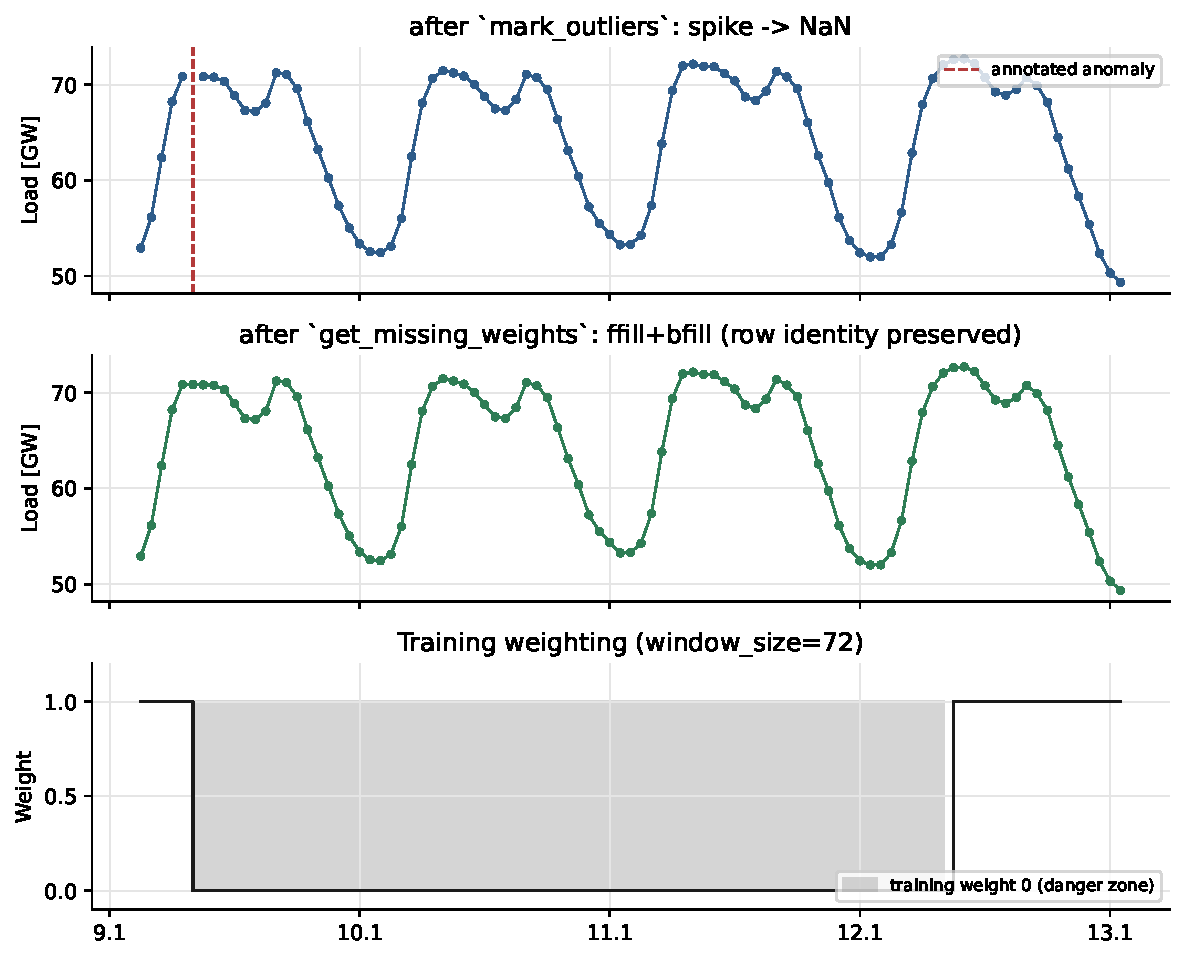
\includegraphics[keepaspectratio]{03_data_annotation_files/figure-pdf/fig-zones-output-1.pdf}}

}

\caption{\label{fig-zones}Annotate instead of impute, illustrated on
hours 195-290 (around the injected spike). Top: the series after
\texttt{mark\_outliers} --- the spike is visible as a NaN gap (red
marker). Middle: the same series after \texttt{get\_missing\_weights}
(ffill+bfill). Bottom: the binary training weight --- the entire
lag-window range after the gap is excluded from the loss with weight 0
(grey area).}

\end{figure}%

The grey area illustrates what \texttt{window\_size=72} means in
practice: after each annotated anomaly, another 72 hours are excluded
from training because the lag operator would read them as a feature
vector. Larger gaps widen the zone accordingly.

\section{Persisting for follow-up
chapters}\label{persisting-for-follow-up-chapters}

The annotation pipeline produces \emph{two} artefacts, both
deterministically reproducible: the imputed series and the corresponding
weight series. Both are written into the cache so that chapter 07
(forecaster training) can read them without re-running the annotation.

\protect\phantomsection\label{persist}
\begin{Shaded}
\begin{Highlighting}[]
\NormalTok{df\_filled.to\_parquet(shared }\OperatorTok{/} \StringTok{"load\_de\_2024\_marked.parquet"}\NormalTok{)}
\NormalTok{weights.to\_frame(}\StringTok{"weight"}\NormalTok{).to\_parquet(shared }\OperatorTok{/} \StringTok{"load\_de\_2024\_weights.parquet"}\NormalTok{)}
\BuiltInTok{print}\NormalTok{(}\StringTok{"Annotated series + weight series persisted."}\NormalTok{)}
\end{Highlighting}
\end{Shaded}

\begin{verbatim}
Annotated series + weight series persisted.
\end{verbatim}

\begin{tcolorbox}[enhanced jigsaw, arc=.35mm, bottomrule=.15mm, bottomtitle=1mm, breakable, colback=white, colbacktitle=quarto-callout-tip-color!10!white, colframe=quarto-callout-tip-color-frame, coltitle=black, left=2mm, leftrule=.75mm, opacityback=0, opacitybacktitle=0.6, rightrule=.15mm, title=\textcolor{quarto-callout-tip-color}{\faLightbulb}\hspace{0.5em}{Exercises (with Claude)}, titlerule=0mm, toprule=.15mm, toptitle=1mm]

\begin{enumerate}
\def\labelenumi{\arabic{enumi}.}
\tightlist
\item
  \emph{Annotate vs.~interpolate on the same spike.} Ask Claude to treat
  the spike injected here with
  \texttt{LinearlyInterpolateTS(on\_missing="ffill\_bfill")} instead and
  compare the resulting histogram of the \texttt{load} column with the
  annotated result. Which strategy shifts the mean less? Which one stays
  structurally closer to Art. 10 of the AI Act?
\item
  \emph{Sensitivity of \texttt{window\_size}.} Have Claude produce a
  table for \texttt{window\_size\ in\ \{24,\ 48,\ 72,\ 168\}} showing
  the share of rows with weight 0. At which window size does the danger
  zone become usefully large in practice, and when is it too large?
\item
  \emph{Test the invariant.} Ask Claude for a \texttt{pytest} test that,
  after \texttt{mark\_outliers} + \texttt{get\_missing\_weights}, checks
  \emph{two} properties simultaneously: (a) the series contains no more
  \texttt{NaN} and (b) every originally annotated row has weight 0 and
  at least one of its \texttt{window\_size} follow-up rows does as well.
  Why is this a \emph{contractual property} and not an implementation
  detail?
\end{enumerate}

\end{tcolorbox}

\bookmarksetup{startatroot}

\chapter{Handle data gaps explicitly}\label{sec-missing}

\begin{tcolorbox}[enhanced jigsaw, arc=.35mm, bottomrule=.15mm, bottomtitle=1mm, breakable, colback=white, colbacktitle=quarto-callout-note-color!10!white, colframe=quarto-callout-note-color-frame, coltitle=black, left=2mm, leftrule=.75mm, opacityback=0, opacitybacktitle=0.6, rightrule=.15mm, title=\textcolor{quarto-callout-note-color}{\faInfo}\hspace{0.5em}{Learning objective}, titlerule=0mm, toprule=.15mm, toptitle=1mm]

You understand why a safety-critical library \emph{by default} raises an
exception on missing values instead of silently interpolating, and you
can correctly apply the three modes \texttt{raise},
\texttt{ffill\_bfill}, \texttt{passthrough} of the class
\texttt{LinearlyInterpolateTS}.

\end{tcolorbox}

\begin{tcolorbox}[enhanced jigsaw, arc=.35mm, bottomrule=.15mm, bottomtitle=1mm, breakable, colback=white, colbacktitle=quarto-callout-important-color!10!white, colframe=quarto-callout-important-color-frame, coltitle=black, left=2mm, leftrule=.75mm, opacityback=0, opacitybacktitle=0.6, rightrule=.15mm, title=\textcolor{quarto-callout-important-color}{\faExclamation}\hspace{0.5em}{Preferred strategy: annotation}, titlerule=0mm, toprule=.15mm, toptitle=1mm]

In safety-critical pipelines the \textbf{annotation} strategy from
Chapter~\ref{sec-annotation} (\texttt{mark\_outliers} +
\texttt{get\_missing\_weights} + \texttt{WeightFunction}) is the
preferred one, because it does not replace gaps with invented values ---
broken rows are consistently excluded from the loss with weight 0. The
linear interpolation shown here remains relevant for three situations:
(1) migration from legacy notebooks, (2) as a follow-up step after a
deliberately \emph{non}-imputing imputer, and (3) when the downstream
processing demands a NaN-free series without an explicit weight series.

\end{tcolorbox}

\section{Why are data gaps an AI Act
topic?}\label{why-are-data-gaps-an-ai-act-topic}

Real sensor data contain gaps. A weather station fails for an hour, an
electricity meter is rebooted, a data export drops an empty field. In a
pure research notebook this is harmless. In a high-risk application
under Annex III of the AI Act --- such as the electric load forecast
that a transmission system operator uses for dispatch --- an
\emph{unnoticed} gap is dangerous. It produces a forecast that is
returned with the same apparent confidence as a forecast without a gap;
the auditor will never notice afterwards.

Code rule \textbf{CR-3} (fail-safe processing) therefore requires:
invalid inputs \emph{explicitly} raise an exception instead of being
silently imputed. The AI Act underpins this discipline in Art. 10(3)
(representativeness, error-freedom, completeness) and Art. 15 (accuracy,
robustness, cybersecurity).

\texttt{pandas}, \texttt{scikit-learn}, \texttt{skforecast},
\texttt{Darts}, \texttt{statsmodels} --- most tools in the Python
ecosystem follow the \emph{``silently keep computing''} pattern.
\texttt{spotforecast2-safe} inverts this default.

\section{\texorpdfstring{The three modes of
\texttt{LinearlyInterpolateTS}}{The three modes of LinearlyInterpolateTS}}\label{the-three-modes-of-linearlyinterpolatets}

Since the major version with the contract switch \texttt{on\_missing},
\texttt{LinearlyInterpolateTS} makes the treatment of remaining NaN
values explicit. The class interpolates \emph{inside} the series
linearly (\texttt{limit\_area="inside"}), so middle gaps are cleanly
closed, while endpoint gaps remain and are handled further according to
the mode:

{\def\LTcaptype{none} % do not increment counter
\begin{longtable}[]{@{}
  >{\raggedright\arraybackslash}p{(\linewidth - 4\tabcolsep) * \real{0.1061}}
  >{\raggedright\arraybackslash}p{(\linewidth - 4\tabcolsep) * \real{0.5922}}
  >{\raggedright\arraybackslash}p{(\linewidth - 4\tabcolsep) * \real{0.3017}}@{}}
\toprule\noalign{}
\begin{minipage}[b]{\linewidth}\raggedright
Mode
\end{minipage} & \begin{minipage}[b]{\linewidth}\raggedright
Behaviour
\end{minipage} & \begin{minipage}[b]{\linewidth}\raggedright
Who uses this?
\end{minipage} \\
\midrule\noalign{}
\endhead
\bottomrule\noalign{}
\endlastfoot
\texttt{"raise"} (default) & Raises \texttt{ValueError} with a preview
of the first gaps as soon as any NaN values remain after interpolation.
& Safety-critical pipeline; declares CR-3 actively. \\
\texttt{"ffill\_bfill"} & Fills the remaining endpoint gaps by
forward/backward fill. & Migration from legacy notebooks; internally
also part of the forecaster's training contract. \\
\texttt{"passthrough"} & Passes NaN through unchanged; the next step
takes responsibility. & When a downstream imputer
(e.g.~\texttt{WeightedAverageImputation}) handles the gaps
deliberately. \\
\end{longtable}
}

\section{\texorpdfstring{Code in action: the default is
\texttt{raise}}{Code in action: the default is raise}}\label{code-in-action-the-default-is-raise}

\protect\phantomsection\label{load-y}
\begin{Shaded}
\begin{Highlighting}[]
\ImportTok{import}\NormalTok{ numpy }\ImportTok{as}\NormalTok{ np}
\ImportTok{import}\NormalTok{ pandas }\ImportTok{as}\NormalTok{ pd}
\ImportTok{from}\NormalTok{ pathlib }\ImportTok{import}\NormalTok{ Path}

\NormalTok{shared }\OperatorTok{=}\NormalTok{ Path(}\StringTok{"\_cache/shared"}\NormalTok{)}
\NormalTok{y }\OperatorTok{=}\NormalTok{ pd.read\_parquet(shared }\OperatorTok{/} \StringTok{"load\_de\_2024.parquet"}\NormalTok{)[}\StringTok{"load"}\NormalTok{]}
\BuiltInTok{print}\NormalTok{(}\SpecialStringTok{f"}\SpecialCharTok{\{}\BuiltInTok{len}\NormalTok{(y)}\SpecialCharTok{:,\}}\SpecialStringTok{ hours loaded, }\SpecialCharTok{\{}\BuiltInTok{int}\NormalTok{(y.isna().}\BuiltInTok{sum}\NormalTok{())}\SpecialCharTok{\}}\SpecialStringTok{ NaN."}\NormalTok{)}
\end{Highlighting}
\end{Shaded}

\begin{verbatim}
8,783 hours loaded, 0 NaN.
\end{verbatim}

We construct an artificial gap in the middle of the series to see the
mechanism at work:

\protect\phantomsection\label{insert-gap}
\begin{Shaded}
\begin{Highlighting}[]
\NormalTok{y\_with\_gap }\OperatorTok{=}\NormalTok{ y.copy()}
\NormalTok{y\_with\_gap.iloc[}\DecValTok{120}\NormalTok{:}\DecValTok{123}\NormalTok{] }\OperatorTok{=}\NormalTok{ np.nan        }\CommentTok{\# three NaNs in a row}

\BuiltInTok{print}\NormalTok{(}\SpecialStringTok{f"Artificial NaNs: }\SpecialCharTok{\{}\BuiltInTok{int}\NormalTok{(y\_with\_gap.isna().}\BuiltInTok{sum}\NormalTok{())}\SpecialCharTok{\}}\SpecialStringTok{"}\NormalTok{)}
\BuiltInTok{print}\NormalTok{(}\StringTok{"Example:"}\NormalTok{)}
\BuiltInTok{print}\NormalTok{(y\_with\_gap.iloc[}\DecValTok{118}\NormalTok{:}\DecValTok{126}\NormalTok{].to\_string())}
\end{Highlighting}
\end{Shaded}

\begin{verbatim}
Artificial NaNs: 3
Example:
Time (UTC)
2024-01-05 22:00:00+00:00    50415.8475
2024-01-05 23:00:00+00:00    47558.1450
2024-01-06 00:00:00+00:00           NaN
2024-01-06 01:00:00+00:00           NaN
2024-01-06 02:00:00+00:00           NaN
2024-01-06 03:00:00+00:00    44314.0025
2024-01-06 04:00:00+00:00    44637.6075
2024-01-06 05:00:00+00:00    45244.7525
\end{verbatim}

\protect\phantomsection\label{cr3-raise}
\begin{Shaded}
\begin{Highlighting}[]
\ImportTok{from}\NormalTok{ spotforecast2\_safe }\ImportTok{import}\NormalTok{ LinearlyInterpolateTS}

\CommentTok{\# \textasciigrave{}on\_missing\textasciigrave{} is not specified {-}\textgreater{} default \textquotesingle{}raise\textquotesingle{}}
\NormalTok{y\_clean }\OperatorTok{=}\NormalTok{ LinearlyInterpolateTS().fit\_transform(y\_with\_gap)}

\BuiltInTok{print}\NormalTok{(}\SpecialStringTok{f"NaN after interpolation:  }\SpecialCharTok{\{}\BuiltInTok{int}\NormalTok{(y\_clean.isna().}\BuiltInTok{sum}\NormalTok{())}\SpecialCharTok{\}}\SpecialStringTok{"}\NormalTok{)}
\BuiltInTok{print}\NormalTok{(y\_clean.iloc[}\DecValTok{118}\NormalTok{:}\DecValTok{126}\NormalTok{].to\_string())}
\end{Highlighting}
\end{Shaded}

\begin{verbatim}
NaN after interpolation:  0
Time (UTC)
2024-01-05 22:00:00+00:00    50415.847500
2024-01-05 23:00:00+00:00    47558.145000
2024-01-06 00:00:00+00:00    46747.109375
2024-01-06 01:00:00+00:00    45936.073750
2024-01-06 02:00:00+00:00    45125.038125
2024-01-06 03:00:00+00:00    44314.002500
2024-01-06 04:00:00+00:00    44637.607500
2024-01-06 05:00:00+00:00    45244.752500
\end{verbatim}

The middle gap was cleanly closed because values on both sides were
available. The default mode \texttt{raise} only stops \emph{if} NaN
values remain after the interpolation --- typically at the start or end
of the series.

\section{Endpoint gaps: here CR-3 shows its
effect}\label{endpoint-gaps-here-cr-3-shows-its-effect}

\protect\phantomsection\label{cr3-edge}
\begin{Shaded}
\begin{Highlighting}[]
\NormalTok{y\_edge }\OperatorTok{=}\NormalTok{ y.copy()}
\NormalTok{y\_edge.iloc[}\DecValTok{0}\NormalTok{:}\DecValTok{2}\NormalTok{] }\OperatorTok{=}\NormalTok{ np.nan        }\CommentTok{\# the first two hours are missing}

\ControlFlowTok{try}\NormalTok{:}
\NormalTok{    LinearlyInterpolateTS(on\_missing}\OperatorTok{=}\StringTok{"raise"}\NormalTok{).fit\_transform(y\_edge)}
\ControlFlowTok{except} \PreprocessorTok{ValueError} \ImportTok{as}\NormalTok{ exc:}
    \BuiltInTok{print}\NormalTok{(}\StringTok{"Expected fail{-}safe abort:"}\NormalTok{)}
    \BuiltInTok{print}\NormalTok{(}\BuiltInTok{str}\NormalTok{(exc))}
\end{Highlighting}
\end{Shaded}

\begin{verbatim}
Expected fail-safe abort:
2 missing value(s) remain after linear interpolation. First gaps: [2024-01-01 00:00:00+00:00, 2024-01-01 01:00:00+00:00]. Pass on_missing='ffill_bfill' to opt into endpoint forward/backward fill or on_missing='passthrough' to return the interpolated series with residual NaN.
\end{verbatim}

The error message contains a preview of the first gaps --- that is all a
dispatcher or auditor needs to locate the gap precisely. Exactly this
visibility is what Art. 12 of the AI Act (record-keeping) demands:
nothing must fall under the table.

\section{\texorpdfstring{\texttt{ffill\_bfill} as a deliberate
opt-in}{ffill\_bfill as a deliberate opt-in}}\label{ffill_bfill-as-a-deliberate-opt-in}

If you want to tolerate endpoint gaps deliberately (e.g.~at the start of
a migration), you must declare this explicitly:

\protect\phantomsection\label{cr3-ffill}
\begin{Shaded}
\begin{Highlighting}[]
\NormalTok{y\_filled }\OperatorTok{=}\NormalTok{ LinearlyInterpolateTS(on\_missing}\OperatorTok{=}\StringTok{"ffill\_bfill"}\NormalTok{).fit\_transform(y\_edge)}
\BuiltInTok{print}\NormalTok{(}\SpecialStringTok{f"NaN after \textquotesingle{}ffill\_bfill\textquotesingle{}:   }\SpecialCharTok{\{}\BuiltInTok{int}\NormalTok{(y\_filled.isna().}\BuiltInTok{sum}\NormalTok{())}\SpecialCharTok{\}}\SpecialStringTok{"}\NormalTok{)}
\BuiltInTok{print}\NormalTok{(}\StringTok{"First five hours:"}\NormalTok{, y\_filled.iloc[:}\DecValTok{5}\NormalTok{].}\BuiltInTok{round}\NormalTok{(}\DecValTok{2}\NormalTok{).tolist())}
\end{Highlighting}
\end{Shaded}

\begin{verbatim}
NaN after 'ffill_bfill':   0
First five hours: [37123.23, 37123.23, 37123.23, 36753.52, 37051.4]
\end{verbatim}

Internally \texttt{ForecasterRecursiveModel} uses exactly this
configuration in eight places --- not out of carelessness, but to
satisfy the training invariant ``no NaN in the lag window at training
time'' even when the caller passes the series without pre-processing.
The contract is made visible at the call site; that is the difference
from silent imputation.

\section{\texorpdfstring{\texttt{passthrough}: responsibility passed to
the
caller}{passthrough: responsibility passed to the caller}}\label{passthrough-responsibility-passed-to-the-caller}

\protect\phantomsection\label{cr3-passthrough}
\begin{Shaded}
\begin{Highlighting}[]
\NormalTok{y\_pt }\OperatorTok{=}\NormalTok{ LinearlyInterpolateTS(on\_missing}\OperatorTok{=}\StringTok{"passthrough"}\NormalTok{).fit\_transform(y\_edge)}
\BuiltInTok{print}\NormalTok{(}\SpecialStringTok{f"NaN after \textquotesingle{}passthrough\textquotesingle{}:  }\SpecialCharTok{\{}\BuiltInTok{int}\NormalTok{(y\_pt.isna().}\BuiltInTok{sum}\NormalTok{())}\SpecialCharTok{\}}\SpecialStringTok{"}\NormalTok{)}
\end{Highlighting}
\end{Shaded}

\begin{verbatim}
NaN after 'passthrough':  2
\end{verbatim}

Useful, for example, when a downstream
\texttt{WeightedAverageImputation} step fills the gaps deliberately. The
\texttt{WARNING} emitted by that imputer is shown so that the caller
sees in the audit log that imputation has happened.

\section{Visualisation: before/after picture of gap
handling}\label{visualisation-beforeafter-picture-of-gap-handling}

\begin{Shaded}
\begin{Highlighting}[]
\ImportTok{import}\NormalTok{ matplotlib.pyplot }\ImportTok{as}\NormalTok{ plt}
\ImportTok{import}\NormalTok{ matplotlib.dates }\ImportTok{as}\NormalTok{ mdates}

\NormalTok{window }\OperatorTok{=} \BuiltInTok{slice}\NormalTok{(}\DecValTok{115}\NormalTok{, }\DecValTok{130}\NormalTok{)}
\NormalTok{fig, (ax\_top, ax\_bot) }\OperatorTok{=}\NormalTok{ plt.subplots(}\DecValTok{2}\NormalTok{, }\DecValTok{1}\NormalTok{, figsize}\OperatorTok{=}\NormalTok{(}\FloatTok{8.0}\NormalTok{, }\FloatTok{4.5}\NormalTok{), sharex}\OperatorTok{=}\VariableTok{True}\NormalTok{)}

\NormalTok{ax\_top.plot(y\_with\_gap.iloc[window].index, y\_with\_gap.iloc[window].values }\OperatorTok{/} \DecValTok{1000}\NormalTok{,}
            \StringTok{"o{-}"}\NormalTok{, color}\OperatorTok{=}\StringTok{"\#B33A3A"}\NormalTok{, linewidth}\OperatorTok{=}\FloatTok{1.0}\NormalTok{, markersize}\OperatorTok{=}\DecValTok{4}\NormalTok{)}
\NormalTok{ax\_top.set\_ylabel(}\StringTok{"Load [GW]"}\NormalTok{)}
\NormalTok{ax\_top.set\_title(}\StringTok{"before interpolation: three NaN"}\NormalTok{)}
\NormalTok{ax\_top.grid(}\VariableTok{True}\NormalTok{, color}\OperatorTok{=}\StringTok{"\#E5E5E5"}\NormalTok{, linewidth}\OperatorTok{=}\FloatTok{0.5}\NormalTok{)}

\NormalTok{ax\_bot.plot(y\_clean.iloc[window].index, y\_clean.iloc[window].values }\OperatorTok{/} \DecValTok{1000}\NormalTok{,}
            \StringTok{"o{-}"}\NormalTok{, color}\OperatorTok{=}\StringTok{"\#2E7D55"}\NormalTok{, linewidth}\OperatorTok{=}\FloatTok{1.0}\NormalTok{, markersize}\OperatorTok{=}\DecValTok{4}\NormalTok{)}
\NormalTok{ax\_bot.set\_ylabel(}\StringTok{"Load [GW]"}\NormalTok{)}
\NormalTok{ax\_bot.set\_title(}\StringTok{"after \textasciigrave{}LinearlyInterpolateTS()\textasciigrave{} (default \textasciigrave{}on\_missing=\textquotesingle{}raise\textquotesingle{}\textasciigrave{})"}\NormalTok{)}
\NormalTok{ax\_bot.grid(}\VariableTok{True}\NormalTok{, color}\OperatorTok{=}\StringTok{"\#E5E5E5"}\NormalTok{, linewidth}\OperatorTok{=}\FloatTok{0.5}\NormalTok{)}
\NormalTok{ax\_bot.xaxis.set\_major\_locator(mdates.HourLocator(byhour}\OperatorTok{=}\NormalTok{[}\DecValTok{0}\NormalTok{, }\DecValTok{12}\NormalTok{]))}
\NormalTok{ax\_bot.xaxis.set\_major\_formatter(mdates.DateFormatter(}\StringTok{"}\SpecialCharTok{\%{-}d}\StringTok{.\%{-}m \%H:\%M"}\NormalTok{))}

\ControlFlowTok{for}\NormalTok{ ax }\KeywordTok{in}\NormalTok{ (ax\_top, ax\_bot):}
    \ControlFlowTok{for}\NormalTok{ s }\KeywordTok{in}\NormalTok{ (}\StringTok{"top"}\NormalTok{, }\StringTok{"right"}\NormalTok{):}
\NormalTok{        ax.spines[s].set\_visible(}\VariableTok{False}\NormalTok{)}

\NormalTok{fig.tight\_layout()}
\NormalTok{plt.show()}
\end{Highlighting}
\end{Shaded}

\begin{figure}[H]

\centering{

\pandocbounded{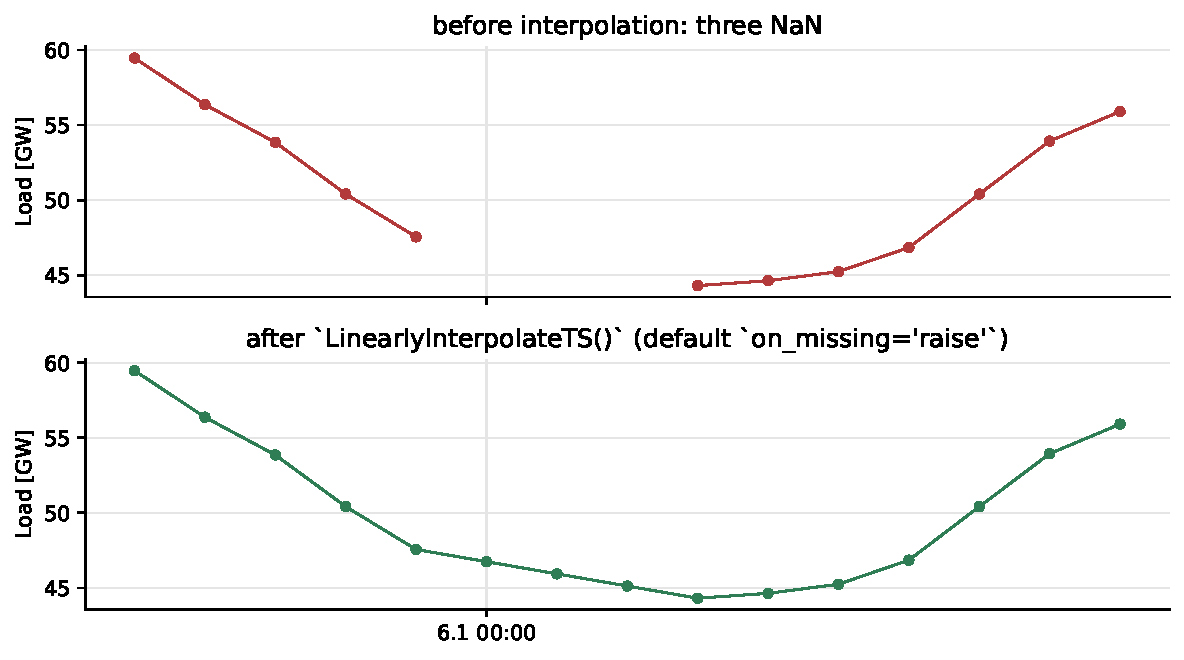
\includegraphics[keepaspectratio]{04_missing_data_files/figure-pdf/fig-gap-fill-output-1.pdf}}

}

\caption{\label{fig-gap-fill}Demonstration of the
\texttt{LinearlyInterpolateTS} treatment. Top: an artificially injected
gap (three consecutive NaN values) in January 2024. Bottom: the same
series after the default call with
\texttt{on\_missing=\textquotesingle{}raise\textquotesingle{}} --- the
three NaNs are filled in by linear interpolation of the neighbouring
values; because no endpoint gaps remain, no error is raised.}

\end{figure}%

\section{Which strategy when? --- a comparison at a
glance}\label{which-strategy-when-a-comparison-at-a-glance}

The three \texttt{LinearlyInterpolateTS} modes and the annotation
pipeline from Chapter~\ref{sec-annotation} are not mutually exclusive
--- they target different points in the lifecycle of the data. Before
mapping the application situations, a direct comparison of the two
strategies' \emph{structural properties} is worthwhile:

{\def\LTcaptype{none} % do not increment counter
\begin{longtable}[]{@{}
  >{\raggedright\arraybackslash}p{(\linewidth - 4\tabcolsep) * \real{0.2774}}
  >{\raggedright\arraybackslash}p{(\linewidth - 4\tabcolsep) * \real{0.3419}}
  >{\raggedright\arraybackslash}p{(\linewidth - 4\tabcolsep) * \real{0.3806}}@{}}
\toprule\noalign{}
\begin{minipage}[b]{\linewidth}\raggedright
Property
\end{minipage} & \begin{minipage}[b]{\linewidth}\raggedright
\texttt{LinearlyInterpolateTS}
\end{minipage} & \begin{minipage}[b]{\linewidth}\raggedright
\texttt{mark\_outliers} + \texttt{get\_missing\_weights}
(Chapter~\ref{sec-annotation})
\end{minipage} \\
\midrule\noalign{}
\endhead
\bottomrule\noalign{}
\endlastfoot
Series length after pre-processing & unchanged & unchanged \\
NaN guarantee after the step & only in \texttt{ffill\_bfill} mode /
after interpolation & yes, guaranteed after
\texttt{get\_missing\_weights} \\
Training target contains invented values & yes (line between neighbours)
& no (real values; broken values are ffill placeholders with weight
0) \\
Auditability of the action & indirect (\texttt{raise} error message) &
direct (\texttt{verbose=True} lists indices; \texttt{weights} is
serialisable) \\
Model bias due to imputation & possible & structurally excluded (weight
0) \\
Recommendation for high-risk applications & only as a migration path or
with a downstream imputer & \textbf{standard strategy} \\
\end{longtable}
}

The following table translates these structural differences into
concrete application situations:

{\def\LTcaptype{none} % do not increment counter
\begin{longtable}[]{@{}
  >{\raggedright\arraybackslash}p{(\linewidth - 2\tabcolsep) * \real{0.5299}}
  >{\raggedright\arraybackslash}p{(\linewidth - 2\tabcolsep) * \real{0.4701}}@{}}
\toprule\noalign{}
\begin{minipage}[b]{\linewidth}\raggedright
Situation
\end{minipage} & \begin{minipage}[b]{\linewidth}\raggedright
Recommended strategy
\end{minipage} \\
\midrule\noalign{}
\endhead
\bottomrule\noalign{}
\endlastfoot
Production high-risk pipeline (Annex III) & \textbf{Annotation}
(Chapter~\ref{sec-annotation}); interpolation only as a downstream
special step \\
Middle gaps of individual hours, no systematic outlier search needed &
\texttt{LinearlyInterpolateTS(on\_missing="raise")} as a CR-3 switch \\
Migration from legacy notebooks without a \texttt{weight\_func} path &
\texttt{LinearlyInterpolateTS(on\_missing="ffill\_bfill")} as a
bridge \\
Own downstream imputer &
\texttt{LinearlyInterpolateTS(on\_missing="passthrough")} \\
Audit requires an explicit, picklable weight series &
\textbf{Annotation} (Chapter~\ref{sec-annotation}); weights are part of
the model artefact \\
\end{longtable}
}

If in doubt, start with the annotation from Chapter~\ref{sec-annotation}
and only fall back to \texttt{LinearlyInterpolateTS} when there is a
concrete argument against the weight series.

\section{Persisting for follow-up
chapters}\label{persisting-for-follow-up-chapters-1}

We take the clean series as the starting point for all the following
steps:

\protect\phantomsection\label{persist-clean}
\begin{Shaded}
\begin{Highlighting}[]
\NormalTok{y\_clean.to\_frame(}\StringTok{"load"}\NormalTok{).to\_parquet(shared }\OperatorTok{/} \StringTok{"load\_de\_2024\_clean.parquet"}\NormalTok{)}
\BuiltInTok{print}\NormalTok{(}\StringTok{"Cleaned series persisted."}\NormalTok{)}
\end{Highlighting}
\end{Shaded}

\begin{verbatim}
Cleaned series persisted.
\end{verbatim}

\begin{tcolorbox}[enhanced jigsaw, arc=.35mm, bottomrule=.15mm, bottomtitle=1mm, breakable, colback=white, colbacktitle=quarto-callout-tip-color!10!white, colframe=quarto-callout-tip-color-frame, coltitle=black, left=2mm, leftrule=.75mm, opacityback=0, opacitybacktitle=0.6, rightrule=.15mm, title=\textcolor{quarto-callout-tip-color}{\faLightbulb}\hspace{0.5em}{Exercises (with Claude)}, titlerule=0mm, toprule=.15mm, toptitle=1mm]

\begin{enumerate}
\def\labelenumi{\arabic{enumi}.}
\tightlist
\item
  \emph{Three modes on the same example.} Ask Claude to write a small
  comparison table showing, for the three modes \texttt{raise},
  \texttt{ffill\_bfill}, \texttt{passthrough} on a series with
  \emph{both} a middle and an endpoint gap, what the result looks like
  in each case. Which mode is directly compatible with Art. 10 of the AI
  Act?
\item
  \emph{Comparison with pandas.} Have Claude compare
  \texttt{pandas.Series.interpolate()} directly with
  \texttt{LinearlyInterpolateTS(on\_missing=\textquotesingle{}raise\textquotesingle{})}.
  On an example with gaps at the edge: what happens in each variant?
  Which default is more suitable for a safety-critical pipeline?
\item
  \emph{Test the contract.} Ask Claude how you would write a \emph{test}
  that, in a CI pipeline, ensures that \texttt{LinearlyInterpolateTS()}
  (without an explicit argument) preserves the default
  \texttt{on\_missing=\textquotesingle{}raise\textquotesingle{}}. Argue
  why this property must be tested as a \emph{contract} --- and not just
  stated in the documentation.
\end{enumerate}

\end{tcolorbox}

\bookmarksetup{startatroot}

\chapter{Separating training and evaluation range}\label{sec-split}

\begin{tcolorbox}[enhanced jigsaw, arc=.35mm, bottomrule=.15mm, bottomtitle=1mm, breakable, colback=white, colbacktitle=quarto-callout-note-color!10!white, colframe=quarto-callout-note-color-frame, coltitle=black, left=2mm, leftrule=.75mm, opacityback=0, opacitybacktitle=0.6, rightrule=.15mm, title=\textcolor{quarto-callout-note-color}{\faInfo}\hspace{0.5em}{Learning objective}, titlerule=0mm, toprule=.15mm, toptitle=1mm]

You understand why a random split is wrong for time series, and you can
perform a clean chronological train/test split.

\end{tcolorbox}

\section{Why not split randomly?}\label{why-not-split-randomly}

In classical supervised learning (e.g.~image classification) the dataset
is split randomly into training and test ranges. For \emph{time series}
this is a mistake: every value knows its past, and a randomly drawn
training set would contain \emph{future} hours from which the model
implicitly learns to predict \emph{past} hours. The accuracy measurement
would be self-deception; it would collapse dramatically in live
operation.

We therefore split \emph{chronologically}: a contiguous initial segment
is used for training, a contiguous final segment for evaluation. This
split is the simplest variant of a representativeness check demanded by
Art. 10(2)(f) and (g) of the AI Act. Code rule \textbf{CR-2}
(determinism) additionally requires the cut point to be fixed as a
constant --- not random, but reproducible.

\section{Code in action}\label{code-in-action-2}

We take the series cleaned in Chapter~\ref{sec-missing} and define
January to October 2024 as the training range and November as the
evaluation range.

\protect\phantomsection\label{split-data}
\begin{Shaded}
\begin{Highlighting}[]
\ImportTok{import}\NormalTok{ pandas }\ImportTok{as}\NormalTok{ pd}
\ImportTok{from}\NormalTok{ pathlib }\ImportTok{import}\NormalTok{ Path}

\NormalTok{shared }\OperatorTok{=}\NormalTok{ Path(}\StringTok{"\_cache/shared"}\NormalTok{)}
\NormalTok{y\_clean }\OperatorTok{=}\NormalTok{ pd.read\_parquet(shared }\OperatorTok{/} \StringTok{"load\_de\_2024\_clean.parquet"}\NormalTok{)[}\StringTok{"load"}\NormalTok{]}

\NormalTok{TRAIN\_END }\OperatorTok{=}\NormalTok{ pd.Timestamp(}\StringTok{"2024{-}10{-}31 23:00"}\NormalTok{, tz}\OperatorTok{=}\StringTok{"UTC"}\NormalTok{)}
\NormalTok{EVAL\_END  }\OperatorTok{=}\NormalTok{ pd.Timestamp(}\StringTok{"2024{-}11{-}30 23:00"}\NormalTok{, tz}\OperatorTok{=}\StringTok{"UTC"}\NormalTok{)}

\NormalTok{y\_train }\OperatorTok{=}\NormalTok{ y\_clean.loc[:TRAIN\_END]}
\NormalTok{y\_eval  }\OperatorTok{=}\NormalTok{ y\_clean.loc[TRAIN\_END }\OperatorTok{+}\NormalTok{ pd.Timedelta(hours}\OperatorTok{=}\DecValTok{1}\NormalTok{) : EVAL\_END]}

\BuiltInTok{print}\NormalTok{(}\SpecialStringTok{f"Training:    }\SpecialCharTok{\{}\NormalTok{y\_train}\SpecialCharTok{.}\NormalTok{index[}\DecValTok{0}\NormalTok{]}\SpecialCharTok{\}}\SpecialStringTok{  to  }\SpecialCharTok{\{}\NormalTok{y\_train}\SpecialCharTok{.}\NormalTok{index[}\OperatorTok{{-}}\DecValTok{1}\NormalTok{]}\SpecialCharTok{\}}\SpecialStringTok{  "}
      \SpecialStringTok{f"(}\SpecialCharTok{\{}\BuiltInTok{len}\NormalTok{(y\_train)}\SpecialCharTok{:,\}}\SpecialStringTok{ h)"}\NormalTok{)}
\BuiltInTok{print}\NormalTok{(}\SpecialStringTok{f"Evaluation:  }\SpecialCharTok{\{}\NormalTok{y\_eval}\SpecialCharTok{.}\NormalTok{index[}\DecValTok{0}\NormalTok{]}\SpecialCharTok{\}}\SpecialStringTok{  to  }\SpecialCharTok{\{}\NormalTok{y\_eval}\SpecialCharTok{.}\NormalTok{index[}\OperatorTok{{-}}\DecValTok{1}\NormalTok{]}\SpecialCharTok{\}}\SpecialStringTok{  "}
      \SpecialStringTok{f"(}\SpecialCharTok{\{}\BuiltInTok{len}\NormalTok{(y\_eval)}\SpecialCharTok{:,\}}\SpecialStringTok{ h)"}\NormalTok{)}
\end{Highlighting}
\end{Shaded}

\begin{verbatim}
Training:    2024-01-01 00:00:00+00:00  to  2024-10-31 23:00:00+00:00  (7,320 h)
Evaluation:  2024-11-01 00:00:00+00:00  to  2024-11-30 23:00:00+00:00  (720 h)
\end{verbatim}

We persist the cut points so that all following chapters use exactly the
same split:

\begin{Shaded}
\begin{Highlighting}[]
\NormalTok{y\_train.to\_frame(}\StringTok{"load"}\NormalTok{).to\_parquet(shared }\OperatorTok{/} \StringTok{"y\_train.parquet"}\NormalTok{)}
\NormalTok{y\_eval.to\_frame(}\StringTok{"load"}\NormalTok{).to\_parquet(shared }\OperatorTok{/} \StringTok{"y\_eval.parquet"}\NormalTok{)}
\NormalTok{(shared }\OperatorTok{/} \StringTok{"split\_meta.json"}\NormalTok{).write\_text(}
    \SpecialStringTok{f\textquotesingle{}}\CharTok{\{\{}\SpecialStringTok{"train\_end":"}\SpecialCharTok{\{}\NormalTok{TRAIN\_END}\SpecialCharTok{.}\NormalTok{isoformat()}\SpecialCharTok{\}}\SpecialStringTok{",\textquotesingle{}}
    \SpecialStringTok{f\textquotesingle{}"eval\_end":"}\SpecialCharTok{\{}\NormalTok{EVAL\_END}\SpecialCharTok{.}\NormalTok{isoformat()}\SpecialCharTok{\}}\SpecialStringTok{",\textquotesingle{}}
    \SpecialStringTok{f\textquotesingle{}"freq":"h","tz":"UTC"}\CharTok{\}\}}\SpecialStringTok{\textquotesingle{}}
\NormalTok{)}
\end{Highlighting}
\end{Shaded}

\protect\phantomsection\label{persist-split}
\begin{verbatim}
102
\end{verbatim}

\section{Visualisation: the split on the time
axis}\label{visualisation-the-split-on-the-time-axis}

\begin{Shaded}
\begin{Highlighting}[]
\ImportTok{import}\NormalTok{ matplotlib.pyplot }\ImportTok{as}\NormalTok{ plt}
\ImportTok{import}\NormalTok{ matplotlib.dates }\ImportTok{as}\NormalTok{ mdates}
\ImportTok{import}\NormalTok{ matplotlib.patches }\ImportTok{as}\NormalTok{ mpatches}

\NormalTok{fig, ax }\OperatorTok{=}\NormalTok{ plt.subplots(figsize}\OperatorTok{=}\NormalTok{(}\FloatTok{8.5}\NormalTok{, }\FloatTok{3.0}\NormalTok{))}
\NormalTok{ax.plot(y\_train.index, y\_train.values }\OperatorTok{/} \DecValTok{1000}\NormalTok{,}
\NormalTok{        color}\OperatorTok{=}\StringTok{"\#1F4E79"}\NormalTok{, linewidth}\OperatorTok{=}\FloatTok{0.4}\NormalTok{, label}\OperatorTok{=}\StringTok{"Training"}\NormalTok{)}
\NormalTok{ax.plot(y\_eval.index, y\_eval.values }\OperatorTok{/} \DecValTok{1000}\NormalTok{,}
\NormalTok{        color}\OperatorTok{=}\StringTok{"\#E07B00"}\NormalTok{, linewidth}\OperatorTok{=}\FloatTok{0.6}\NormalTok{, label}\OperatorTok{=}\StringTok{"Evaluation"}\NormalTok{)}

\NormalTok{reserve\_idx }\OperatorTok{=}\NormalTok{ y\_clean.loc[EVAL\_END }\OperatorTok{+}\NormalTok{ pd.Timedelta(hours}\OperatorTok{=}\DecValTok{1}\NormalTok{):].index}
\NormalTok{ax.plot(reserve\_idx, y\_clean.loc[reserve\_idx].values }\OperatorTok{/} \DecValTok{1000}\NormalTok{,}
\NormalTok{        color}\OperatorTok{=}\StringTok{"\#999999"}\NormalTok{, linewidth}\OperatorTok{=}\FloatTok{0.4}\NormalTok{, label}\OperatorTok{=}\StringTok{"Reserve"}\NormalTok{)}

\NormalTok{ax.axvline(TRAIN\_END, color}\OperatorTok{=}\StringTok{"\#555555"}\NormalTok{, linestyle}\OperatorTok{=}\StringTok{"{-}{-}"}\NormalTok{, linewidth}\OperatorTok{=}\FloatTok{0.7}\NormalTok{)}
\NormalTok{ax.axvline(EVAL\_END,  color}\OperatorTok{=}\StringTok{"\#555555"}\NormalTok{, linestyle}\OperatorTok{=}\StringTok{"{-}{-}"}\NormalTok{, linewidth}\OperatorTok{=}\FloatTok{0.7}\NormalTok{)}
\NormalTok{ax.set\_ylabel(}\StringTok{"Load [GW]"}\NormalTok{)}
\NormalTok{ax.set\_xlabel(}\StringTok{"Time"}\NormalTok{)}
\NormalTok{ax.grid(}\VariableTok{True}\NormalTok{, color}\OperatorTok{=}\StringTok{"\#E5E5E5"}\NormalTok{, linewidth}\OperatorTok{=}\FloatTok{0.5}\NormalTok{)}
\NormalTok{ax.xaxis.set\_major\_locator(mdates.MonthLocator())}
\NormalTok{ax.xaxis.set\_major\_formatter(mdates.DateFormatter(}\StringTok{"\%b \%Y"}\NormalTok{))}
\NormalTok{ax.legend(loc}\OperatorTok{=}\StringTok{"upper left"}\NormalTok{, frameon}\OperatorTok{=}\VariableTok{False}\NormalTok{)}
\ControlFlowTok{for}\NormalTok{ s }\KeywordTok{in}\NormalTok{ (}\StringTok{"top"}\NormalTok{, }\StringTok{"right"}\NormalTok{):}
\NormalTok{    ax.spines[s].set\_visible(}\VariableTok{False}\NormalTok{)}
\NormalTok{fig.tight\_layout()}
\NormalTok{plt.show()}
\end{Highlighting}
\end{Shaded}

\begin{figure}[H]

\centering{

\pandocbounded{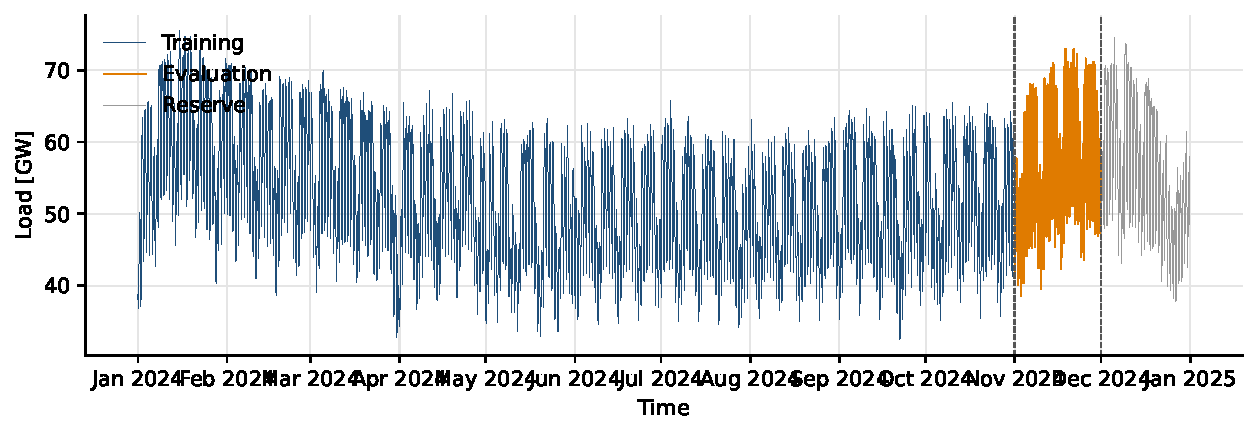
\includegraphics[keepaspectratio]{05_train_test_split_files/figure-pdf/fig-split-output-1.pdf}}

}

\caption{\label{fig-split}Chronological train/test split of the cleaned
2024 load series. Training range (blue): January to October. Evaluation
range (orange): November. December (grey) is held back as a reserve for
future follow-up experiments. The dashed line marks the cut point.}

\end{figure}%

\begin{tcolorbox}[enhanced jigsaw, arc=.35mm, bottomrule=.15mm, bottomtitle=1mm, breakable, colback=white, colbacktitle=quarto-callout-tip-color!10!white, colframe=quarto-callout-tip-color-frame, coltitle=black, left=2mm, leftrule=.75mm, opacityback=0, opacitybacktitle=0.6, rightrule=.15mm, title=\textcolor{quarto-callout-tip-color}{\faLightbulb}\hspace{0.5em}{Exercises (with Claude)}, titlerule=0mm, toprule=.15mm, toptitle=1mm]

\begin{enumerate}
\def\labelenumi{\arabic{enumi}.}
\tightlist
\item
  \emph{Why chronologically?} Have Claude show on a small concrete
  example (e.g.~a 10-value series) what goes wrong if you split randomly
  instead of chronologically. Which metrics from Art. 15 of the AI Act
  are thereby falsified?
\item
  \emph{Cut point as contract.} Discuss with Claude why
  \texttt{TRAIN\_END} should live as a \emph{constant} in a separate
  file (or at the very top of the notebook) rather than being scattered
  through the code. Which code rule does this practice follow?
\item
  \emph{Robustness.} Ask Claude to show a variant in which the split is
  not performed once but multiple times at different cut-off dates (e.g.
  monthly rolling). How does the informativeness of the accuracy
  measurement change?
\end{enumerate}

\end{tcolorbox}

\bookmarksetup{startatroot}

\chapter{Calendar features and real weather data}\label{sec-calendar}

\begin{tcolorbox}[enhanced jigsaw, arc=.35mm, bottomrule=.15mm, bottomtitle=1mm, breakable, colback=white, colbacktitle=quarto-callout-note-color!10!white, colframe=quarto-callout-note-color-frame, coltitle=black, left=2mm, leftrule=.75mm, opacityback=0, opacitybacktitle=0.6, rightrule=.15mm, title=\textcolor{quarto-callout-note-color}{\faInfo}\hspace{0.5em}{Learning objective}, titlerule=0mm, toprule=.15mm, toptitle=1mm]

You can set up an \texttt{ExogBuilder} with cyclic RBF features, read
real weather data from Open-Meteo via the \texttt{WeatherService} class,
and concatenate both into a single feature matrix that is later passed
to the forecaster as \emph{exogenous input}.

\end{tcolorbox}

\section{Why does the model need more than the load
itself?}\label{why-does-the-model-need-more-than-the-load-itself}

The load depends not only on its own immediate history but also on
\emph{context information}: time of day, day of week, holiday, weather.
If the model only sees ``Wednesday 18:00'' and ``Wednesday 02:00'' as
hours 18 and 2, it has no way to recognise that these hours stand in a
cyclic relationship to each other and repeat periodically. We encode
such cyclic features with \emph{radial basis functions} (RBF) so that an
hour is always similar to its neighbouring hours --- including the
midnight transition.

Weather is the second pillar. In cold weather the load rises (heating,
lighting); on sunny summer days it falls. The model therefore sees per
hour a tuple of hourly temperature, cloud cover, precipitation and wind
speed. The Open-Meteo API provides these values both retrospectively
(archive) and prospectively (forecast) without an API key.

\section{AI Act link}\label{ai-act-link-2}

Art. 10(1) of the AI Act requires that ``training, validation and
testing data sets {[}\ldots{]} meet the quality criteria laid down in
paragraphs 2 to 4''. One of the quality requirements is
\emph{representativeness}: the model must have seen all relevant
seasonal, calendar-related and weather-dependent variations. By training
the load jointly with calendar and weather features, we practically
deliver the ``examination of statistically probable characteristics''
demanded by Art. 10(2)(f).

\texttt{WeatherService} enforces code rule \textbf{CR-3}: any gap in the
weather data that remains after resampling is reported as
\texttt{ValueError} --- not silently filled.

\section{Code in action: cyclic calendar
features}\label{code-in-action-cyclic-calendar-features}

\protect\phantomsection\label{cal-features}
\begin{Shaded}
\begin{Highlighting}[]
\ImportTok{import}\NormalTok{ pandas }\ImportTok{as}\NormalTok{ pd}
\ImportTok{from}\NormalTok{ pathlib }\ImportTok{import}\NormalTok{ Path}
\ImportTok{from}\NormalTok{ spotforecast2\_safe }\ImportTok{import}\NormalTok{ Period, ExogBuilder}

\NormalTok{shared }\OperatorTok{=}\NormalTok{ Path(}\StringTok{"\_cache/shared"}\NormalTok{)}
\NormalTok{y\_train }\OperatorTok{=}\NormalTok{ pd.read\_parquet(shared }\OperatorTok{/} \StringTok{"y\_train.parquet"}\NormalTok{)[}\StringTok{"load"}\NormalTok{]}
\NormalTok{y\_eval  }\OperatorTok{=}\NormalTok{ pd.read\_parquet(shared }\OperatorTok{/} \StringTok{"y\_eval.parquet"}\NormalTok{)[}\StringTok{"load"}\NormalTok{]}

\NormalTok{periods }\OperatorTok{=}\NormalTok{ [}
\NormalTok{    Period(name}\OperatorTok{=}\StringTok{"hour"}\NormalTok{,      n\_periods}\OperatorTok{=}\DecValTok{12}\NormalTok{, column}\OperatorTok{=}\StringTok{"hour"}\NormalTok{,      input\_range}\OperatorTok{=}\NormalTok{(}\DecValTok{0}\NormalTok{, }\DecValTok{23}\NormalTok{)),}
\NormalTok{    Period(name}\OperatorTok{=}\StringTok{"dayofweek"}\NormalTok{, n\_periods}\OperatorTok{=}\DecValTok{4}\NormalTok{,  column}\OperatorTok{=}\StringTok{"dayofweek"}\NormalTok{, input\_range}\OperatorTok{=}\NormalTok{(}\DecValTok{0}\NormalTok{,  }\DecValTok{6}\NormalTok{)),}
\NormalTok{    Period(name}\OperatorTok{=}\StringTok{"month"}\NormalTok{,     n\_periods}\OperatorTok{=}\DecValTok{12}\NormalTok{, column}\OperatorTok{=}\StringTok{"month"}\NormalTok{,     input\_range}\OperatorTok{=}\NormalTok{(}\DecValTok{1}\NormalTok{, }\DecValTok{12}\NormalTok{)),}
\NormalTok{]}
\NormalTok{builder }\OperatorTok{=}\NormalTok{ ExogBuilder(periods}\OperatorTok{=}\NormalTok{periods, country\_code}\OperatorTok{=}\StringTok{"DE"}\NormalTok{)}
\NormalTok{exog\_cal }\OperatorTok{=}\NormalTok{ builder.build(y\_train.index.}\BuiltInTok{min}\NormalTok{(), y\_eval.index.}\BuiltInTok{max}\NormalTok{())}

\BuiltInTok{print}\NormalTok{(}\SpecialStringTok{f"Calendar features: }\SpecialCharTok{\{}\NormalTok{exog\_cal}\SpecialCharTok{.}\NormalTok{shape[}\DecValTok{0}\NormalTok{]}\SpecialCharTok{:,\}}\SpecialStringTok{ hours, }\SpecialCharTok{\{}\NormalTok{exog\_cal}\SpecialCharTok{.}\NormalTok{shape[}\DecValTok{1}\NormalTok{]}\SpecialCharTok{\}}\SpecialStringTok{ columns"}\NormalTok{)}
\BuiltInTok{print}\NormalTok{(}\SpecialStringTok{f"Columns:           }\SpecialCharTok{\{}\BuiltInTok{list}\NormalTok{(exog\_cal.columns)[:}\DecValTok{6}\NormalTok{]}\SpecialCharTok{\}}\SpecialStringTok{ ..."}\NormalTok{)}
\end{Highlighting}
\end{Shaded}

\begin{verbatim}
Calendar features: 8,040 hours, 30 columns
Columns:           ['hour_0', 'hour_1', 'hour_2', 'hour_3', 'hour_4', 'hour_5'] ...
\end{verbatim}

\begin{Shaded}
\begin{Highlighting}[]
\ImportTok{import}\NormalTok{ matplotlib.pyplot }\ImportTok{as}\NormalTok{ plt}

\NormalTok{day }\OperatorTok{=}\NormalTok{ exog\_cal.loc[}\StringTok{"2024{-}03{-}04 00:00"}\NormalTok{:}\StringTok{"2024{-}03{-}04 23:00"}\NormalTok{]}
\NormalTok{fig, ax }\OperatorTok{=}\NormalTok{ plt.subplots(figsize}\OperatorTok{=}\NormalTok{(}\FloatTok{8.5}\NormalTok{, }\FloatTok{3.0}\NormalTok{))}
\NormalTok{hour\_cols }\OperatorTok{=}\NormalTok{ [c }\ControlFlowTok{for}\NormalTok{ c }\KeywordTok{in}\NormalTok{ day.columns }\ControlFlowTok{if}\NormalTok{ c.startswith(}\StringTok{"hour\_"}\NormalTok{)]}
\ControlFlowTok{for}\NormalTok{ c }\KeywordTok{in}\NormalTok{ hour\_cols:}
\NormalTok{    ax.plot(}\BuiltInTok{range}\NormalTok{(}\DecValTok{24}\NormalTok{), day[c].values, linewidth}\OperatorTok{=}\FloatTok{1.0}\NormalTok{, alpha}\OperatorTok{=}\FloatTok{0.7}\NormalTok{)}
\NormalTok{ax.set\_xticks(}\BuiltInTok{range}\NormalTok{(}\DecValTok{0}\NormalTok{, }\DecValTok{24}\NormalTok{, }\DecValTok{2}\NormalTok{))}
\NormalTok{ax.set\_xlabel(}\StringTok{"Hour of day"}\NormalTok{)}
\NormalTok{ax.set\_ylabel(}\StringTok{"RBF activation"}\NormalTok{)}
\NormalTok{ax.set\_title(}\StringTok{"12 cyclic basis functions for the hour of day"}\NormalTok{)}
\NormalTok{ax.grid(}\VariableTok{True}\NormalTok{, color}\OperatorTok{=}\StringTok{"\#E5E5E5"}\NormalTok{, linewidth}\OperatorTok{=}\FloatTok{0.5}\NormalTok{)}
\ControlFlowTok{for}\NormalTok{ s }\KeywordTok{in}\NormalTok{ (}\StringTok{"top"}\NormalTok{, }\StringTok{"right"}\NormalTok{):}
\NormalTok{    ax.spines[s].set\_visible(}\VariableTok{False}\NormalTok{)}
\NormalTok{fig.tight\_layout()}
\NormalTok{plt.show()}
\end{Highlighting}
\end{Shaded}

\begin{figure}[H]

\centering{

\pandocbounded{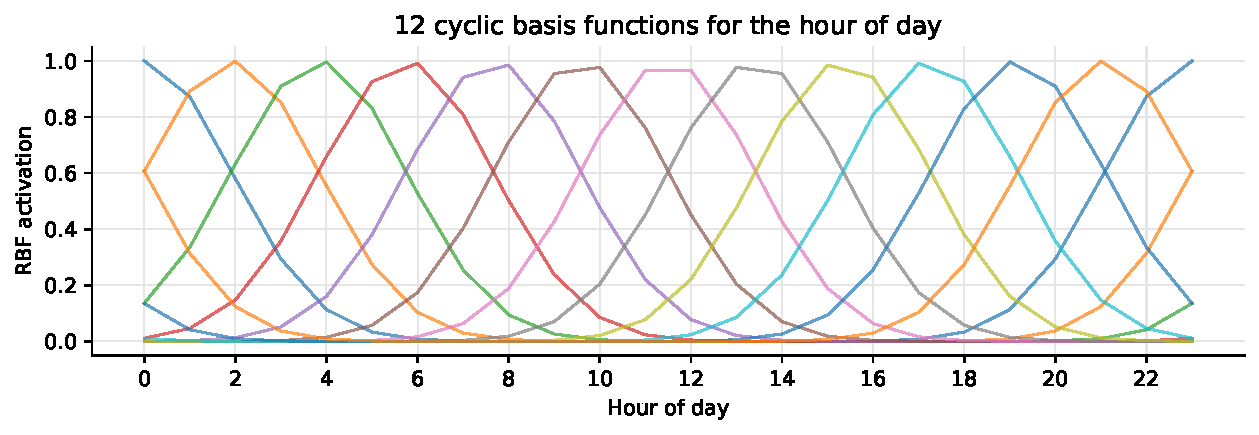
\includegraphics[keepaspectratio]{06_calendar_and_weather_files/figure-pdf/fig-rbf-output-1.pdf}}

}

\caption{\label{fig-rbf}RBF encoding of the hour of day. Each of the 12
basis functions is centred on a different hour. At every position of the
day the activations of all functions sum to one. Midnight is thus `near'
to 23:00 and to 01:00, and the model does not have to learn the jump
between hour 23 and hour 0 artificially.}

\end{figure}%

\section{Code in action: weather}\label{code-in-action-weather}

For a central German location --- Frankfurt am Main, a typical load
centre --- we fetch the hourly values. The \texttt{WeatherService} class
handles the cache transparently: the first request goes to the API,
subsequent identical requests are served from the parquet file.

\protect\phantomsection\label{weather-fetch}
\begin{Shaded}
\begin{Highlighting}[]
\ImportTok{from}\NormalTok{ spotforecast2\_safe.weather }\ImportTok{import}\NormalTok{ WeatherService}

\NormalTok{cache }\OperatorTok{=}\NormalTok{ Path(}\StringTok{"\_cache"}\NormalTok{) }\OperatorTok{/} \StringTok{"weather\_de\_2024.parquet"}
\NormalTok{ws }\OperatorTok{=}\NormalTok{ WeatherService(}
\NormalTok{    latitude}\OperatorTok{=}\FloatTok{50.110924}\NormalTok{,}
\NormalTok{    longitude}\OperatorTok{=}\FloatTok{8.682127}\NormalTok{,}
\NormalTok{    cache\_path}\OperatorTok{=}\NormalTok{cache,}
\NormalTok{    use\_forecast}\OperatorTok{=}\VariableTok{False}\NormalTok{,         }\CommentTok{\# historical data only {-} we stay in 2024}
\NormalTok{)}
\NormalTok{weather }\OperatorTok{=}\NormalTok{ ws.get\_dataframe(}
\NormalTok{    start}\OperatorTok{=}\NormalTok{y\_train.index.}\BuiltInTok{min}\NormalTok{(),}
\NormalTok{    end}\OperatorTok{=}\NormalTok{y\_eval.index.}\BuiltInTok{max}\NormalTok{(),}
\NormalTok{    freq}\OperatorTok{=}\StringTok{"h"}\NormalTok{,}
\NormalTok{    fill\_missing}\OperatorTok{=}\VariableTok{False}\NormalTok{,         }\CommentTok{\# CR{-}3: fail{-}safe, no silent imputation}
\NormalTok{)}
\BuiltInTok{print}\NormalTok{(}\SpecialStringTok{f"Weather frame: }\SpecialCharTok{\{}\NormalTok{weather}\SpecialCharTok{.}\NormalTok{shape[}\DecValTok{0}\NormalTok{]}\SpecialCharTok{:,\}}\SpecialStringTok{ hours, }\SpecialCharTok{\{}\NormalTok{weather}\SpecialCharTok{.}\NormalTok{shape[}\DecValTok{1}\NormalTok{]}\SpecialCharTok{\}}\SpecialStringTok{ columns"}\NormalTok{)}
\BuiltInTok{print}\NormalTok{(}\SpecialStringTok{f"First columns: }\SpecialCharTok{\{}\BuiltInTok{list}\NormalTok{(weather.columns)[:}\DecValTok{5}\NormalTok{]}\SpecialCharTok{\}}\SpecialStringTok{ ..."}\NormalTok{)}
\BuiltInTok{print}\NormalTok{(}\SpecialStringTok{f"NaN values:    }\SpecialCharTok{\{}\BuiltInTok{int}\NormalTok{(weather.isna().}\BuiltInTok{sum}\NormalTok{().}\BuiltInTok{sum}\NormalTok{())}\SpecialCharTok{\}}\SpecialStringTok{ (should be 0; otherwise CR{-}3 would have aborted)"}\NormalTok{)}
\end{Highlighting}
\end{Shaded}

\begin{verbatim}
Weather frame: 8,040 hours, 15 columns
First columns: ['temperature_2m', 'relative_humidity_2m', 'precipitation', 'rain', 'snowfall'] ...
NaN values:    0 (should be 0; otherwise CR-3 would have aborted)
\end{verbatim}

\section{Looking at weather and load
together}\label{looking-at-weather-and-load-together}

\begin{Shaded}
\begin{Highlighting}[]
\ImportTok{import}\NormalTok{ matplotlib.dates }\ImportTok{as}\NormalTok{ mdates}

\NormalTok{window }\OperatorTok{=} \BuiltInTok{slice}\NormalTok{(}\StringTok{"2024{-}03{-}11"}\NormalTok{, }\StringTok{"2024{-}03{-}17"}\NormalTok{)}
\NormalTok{fig, axes }\OperatorTok{=}\NormalTok{ plt.subplots(}\DecValTok{2}\NormalTok{, }\DecValTok{1}\NormalTok{, figsize}\OperatorTok{=}\NormalTok{(}\FloatTok{8.5}\NormalTok{, }\FloatTok{4.5}\NormalTok{), sharex}\OperatorTok{=}\VariableTok{True}\NormalTok{)}

\NormalTok{axes[}\DecValTok{0}\NormalTok{].plot(y\_train.loc[window].index, y\_train.loc[window].values }\OperatorTok{/} \DecValTok{1000}\NormalTok{,}
\NormalTok{             color}\OperatorTok{=}\StringTok{"\#1F4E79"}\NormalTok{, linewidth}\OperatorTok{=}\FloatTok{1.0}\NormalTok{)}
\NormalTok{axes[}\DecValTok{0}\NormalTok{].set\_ylabel(}\StringTok{"Load [GW]"}\NormalTok{)}
\NormalTok{axes[}\DecValTok{0}\NormalTok{].grid(}\VariableTok{True}\NormalTok{, color}\OperatorTok{=}\StringTok{"\#E5E5E5"}\NormalTok{, linewidth}\OperatorTok{=}\FloatTok{0.5}\NormalTok{)}

\NormalTok{axes[}\DecValTok{1}\NormalTok{].plot(weather.loc[window].index, weather.loc[window][}\StringTok{"temperature\_2m"}\NormalTok{].values,}
\NormalTok{             color}\OperatorTok{=}\StringTok{"\#E07B00"}\NormalTok{, linewidth}\OperatorTok{=}\FloatTok{1.0}\NormalTok{)}
\NormalTok{axes[}\DecValTok{1}\NormalTok{].set\_ylabel(}\StringTok{"Temperature [degC]"}\NormalTok{)}
\NormalTok{axes[}\DecValTok{1}\NormalTok{].set\_xlabel(}\StringTok{"Time"}\NormalTok{)}
\NormalTok{axes[}\DecValTok{1}\NormalTok{].grid(}\VariableTok{True}\NormalTok{, color}\OperatorTok{=}\StringTok{"\#E5E5E5"}\NormalTok{, linewidth}\OperatorTok{=}\FloatTok{0.5}\NormalTok{)}
\NormalTok{axes[}\DecValTok{1}\NormalTok{].xaxis.set\_major\_formatter(mdates.DateFormatter(}\StringTok{"\%a }\SpecialCharTok{\%{-}d}\StringTok{.\%{-}m"}\NormalTok{))}

\ControlFlowTok{for}\NormalTok{ ax }\KeywordTok{in}\NormalTok{ axes:}
    \ControlFlowTok{for}\NormalTok{ s }\KeywordTok{in}\NormalTok{ (}\StringTok{"top"}\NormalTok{, }\StringTok{"right"}\NormalTok{):}
\NormalTok{        ax.spines[s].set\_visible(}\VariableTok{False}\NormalTok{)}
\NormalTok{fig.tight\_layout()}
\NormalTok{plt.show()}
\end{Highlighting}
\end{Shaded}

\begin{figure}[H]

\centering{

\pandocbounded{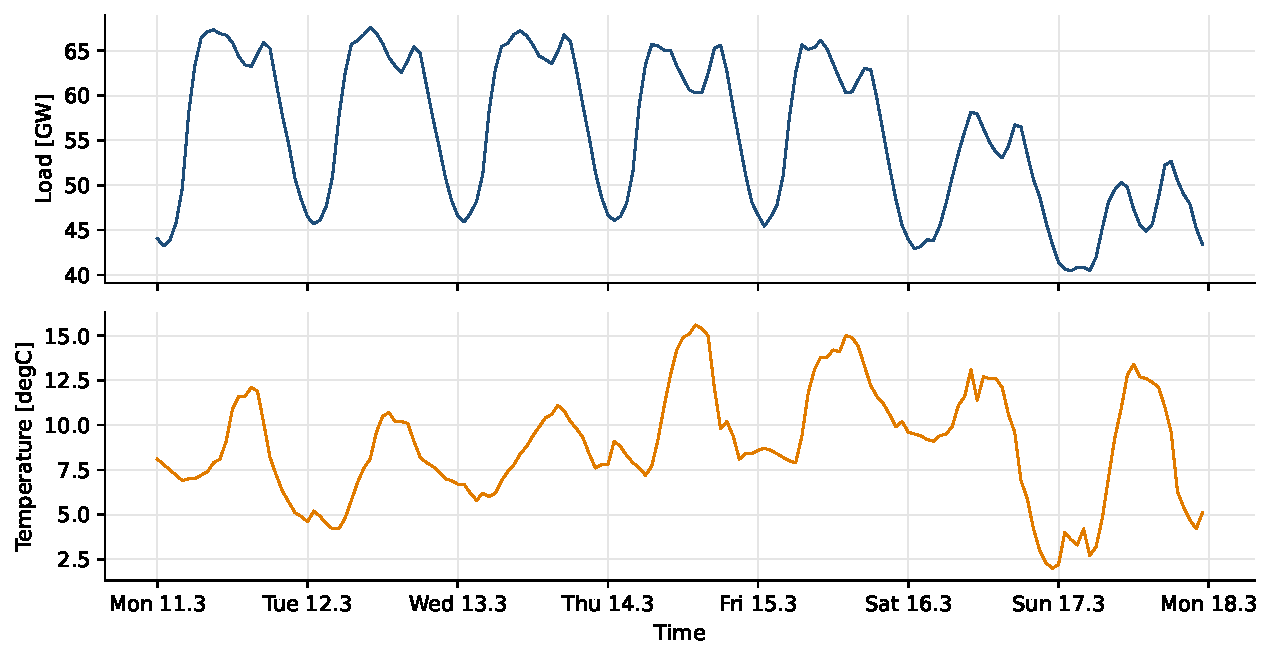
\includegraphics[keepaspectratio]{06_calendar_and_weather_files/figure-pdf/fig-weather-load-output-1.pdf}}

}

\caption{\label{fig-weather-load}Weekly overlay in mid-March 2024:
hourly load (top) and at the same time the 2-metre air temperature in
Frankfurt am Main (bottom). On cold nights the load is visibly higher;
on warm days the midday peak is dampened.}

\end{figure}%

\section{Concatenating calendar and weather into a single
matrix}\label{concatenating-calendar-and-weather-into-a-single-matrix}

The load and the exogenous columns must have exactly the same index,
otherwise the forecaster later fails. This is a direct consequence of
\textbf{CR-3}: missing index rows would silently become NaN inside
\texttt{pandas} --- and that is exactly what we want to avoid.

\protect\phantomsection\label{merge-exog}
\begin{Shaded}
\begin{Highlighting}[]
\NormalTok{exog }\OperatorTok{=}\NormalTok{ exog\_cal.join(weather, how}\OperatorTok{=}\StringTok{"inner"}\NormalTok{)}
\NormalTok{exog }\OperatorTok{=}\NormalTok{ exog.loc[y\_train.index.}\BuiltInTok{min}\NormalTok{(): y\_eval.index.}\BuiltInTok{max}\NormalTok{()]}

\BuiltInTok{print}\NormalTok{(}\SpecialStringTok{f"Joined feature matrix: }\SpecialCharTok{\{}\NormalTok{exog}\SpecialCharTok{.}\NormalTok{shape[}\DecValTok{0}\NormalTok{]}\SpecialCharTok{:,\}}\SpecialStringTok{ hours, }\SpecialCharTok{\{}\NormalTok{exog}\SpecialCharTok{.}\NormalTok{shape[}\DecValTok{1}\NormalTok{]}\SpecialCharTok{\}}\SpecialStringTok{ columns"}\NormalTok{)}
\BuiltInTok{print}\NormalTok{(}\SpecialStringTok{f"NaN values:            }\SpecialCharTok{\{}\BuiltInTok{int}\NormalTok{(exog.isna().}\BuiltInTok{sum}\NormalTok{().}\BuiltInTok{sum}\NormalTok{())}\SpecialCharTok{\}}\SpecialStringTok{"}\NormalTok{)}

\NormalTok{exog.to\_parquet(shared }\OperatorTok{/} \StringTok{"exog.parquet"}\NormalTok{)}
\BuiltInTok{print}\NormalTok{(}\StringTok{"Saved \textasciigrave{}exog.parquet\textasciigrave{} for follow{-}up chapters."}\NormalTok{)}
\end{Highlighting}
\end{Shaded}

\begin{verbatim}
Joined feature matrix: 8,040 hours, 45 columns
NaN values:            0
Saved `exog.parquet` for follow-up chapters.
\end{verbatim}

\begin{tcolorbox}[enhanced jigsaw, arc=.35mm, bottomrule=.15mm, bottomtitle=1mm, breakable, colback=white, colbacktitle=quarto-callout-tip-color!10!white, colframe=quarto-callout-tip-color-frame, coltitle=black, left=2mm, leftrule=.75mm, opacityback=0, opacitybacktitle=0.6, rightrule=.15mm, title=\textcolor{quarto-callout-tip-color}{\faLightbulb}\hspace{0.5em}{Exercises (with Claude)}, titlerule=0mm, toprule=.15mm, toptitle=1mm]

\begin{enumerate}
\def\labelenumi{\arabic{enumi}.}
\tightlist
\item
  \emph{Why RBF?} Ask Claude to show an alternative to the RBF encoding
  (e.g. \texttt{pd.get\_dummies}) and to demonstrate on a plot of the
  midnight transition why this alternative violates cyclic continuity.
\item
  \emph{Weather fail-safe.} Have Claude display the source of
  \texttt{WeatherService.get\_dataframe}, specifically the spot where
  the \texttt{ValueError} is raised when \texttt{fill\_missing=False}.
  What is the exact wording of the error message, and which code rule
  does this behaviour follow?
\item
  \emph{A second city.} Together with Claude extend the pipeline so that
  \emph{two} weather locations (e.g.~Frankfurt and Berlin) are queried
  and both included in the \texttt{exog} matrix with distinct column
  names. Which question could the improved model answer better?
\end{enumerate}

\end{tcolorbox}

\bookmarksetup{startatroot}

\chapter{Instantiate and train the forecaster}\label{sec-train}

\begin{tcolorbox}[enhanced jigsaw, arc=.35mm, bottomrule=.15mm, bottomtitle=1mm, breakable, colback=white, colbacktitle=quarto-callout-note-color!10!white, colframe=quarto-callout-note-color-frame, coltitle=black, left=2mm, leftrule=.75mm, opacityback=0, opacitybacktitle=0.6, rightrule=.15mm, title=\textcolor{quarto-callout-note-color}{\faInfo}\hspace{0.5em}{Learning objective}, titlerule=0mm, toprule=.15mm, toptitle=1mm]

You can instantiate the class \texttt{ForecasterRecursiveLGBM}, equip it
with a deterministically configured LightGBM estimator, and train it on
real load and weather data. You understand why code rules \textbf{CR-2}
(determinism) and \textbf{CR-4} (minimal CVE attack surface) are crucial
in this step.

\end{tcolorbox}

\section{What happens during
training?}\label{what-happens-during-training}

\texttt{ForecasterRecursiveLGBM} is a wrapper around the
gradient-boosting estimator \emph{LightGBM}. During training the model
looks back, for every hour \emph{t}, at the last \texttt{lags} hours
(time steps) and learns a function that predicts the value at hour
\emph{t} from these past values plus the exogenous calendar and weather
features. \emph{Recursive} means: in later prediction the output for
hour \emph{t} is used in turn as input for hour \emph{t+1}.

\texttt{lags=168} (= 7 x 24) means: the model sees the last full week as
context for every hour --- decisive for correctly representing the
weekly rhythm (weekday vs.~weekend).

\section{AI Act link}\label{ai-act-link-3}

Art. 9 of the AI Act demands a risk-management system over the entire
lifecycle; Art. 15 demands an appropriate level of accuracy. Both
obligations presuppose that the training run is \emph{reproducible}: the
supervisory authority must be able to reconstruct the model from its
documented hyperparameters and seed. This is exactly the scope of
\textbf{CR-2}.

\textbf{CR-4} forbids a short negative list of dependencies in the
package (\texttt{plotly}, \texttt{matplotlib}, \texttt{spotoptim},
\texttt{optuna}, \texttt{torch}, \texttt{tensorflow}). The estimator
LightGBM is \emph{not} on this list --- deliberately: it is small,
actively maintained, implemented in C++ and brings no additional attack
surface. A migration to PyTorch or TensorFlow would violate the
deny-list.

\section{Code in action}\label{code-in-action-3}

\protect\phantomsection\label{load-state}
\begin{Shaded}
\begin{Highlighting}[]
\ImportTok{import}\NormalTok{ pandas }\ImportTok{as}\NormalTok{ pd}
\ImportTok{from}\NormalTok{ pathlib }\ImportTok{import}\NormalTok{ Path}

\NormalTok{shared }\OperatorTok{=}\NormalTok{ Path(}\StringTok{"\_cache/shared"}\NormalTok{)}
\NormalTok{y\_train }\OperatorTok{=}\NormalTok{ pd.read\_parquet(shared }\OperatorTok{/} \StringTok{"y\_train.parquet"}\NormalTok{)[}\StringTok{"load"}\NormalTok{]}
\NormalTok{exog    }\OperatorTok{=}\NormalTok{ pd.read\_parquet(shared }\OperatorTok{/} \StringTok{"exog.parquet"}\NormalTok{)}

\BuiltInTok{print}\NormalTok{(}\SpecialStringTok{f"Training series: }\SpecialCharTok{\{}\BuiltInTok{len}\NormalTok{(y\_train)}\SpecialCharTok{:,\}}\SpecialStringTok{ h from }\SpecialCharTok{\{}\NormalTok{y\_train}\SpecialCharTok{.}\NormalTok{index[}\DecValTok{0}\NormalTok{]}\SpecialCharTok{\}}\SpecialStringTok{ to }\SpecialCharTok{\{}\NormalTok{y\_train}\SpecialCharTok{.}\NormalTok{index[}\OperatorTok{{-}}\DecValTok{1}\NormalTok{]}\SpecialCharTok{\}}\SpecialStringTok{"}\NormalTok{)}
\BuiltInTok{print}\NormalTok{(}\SpecialStringTok{f"Exog matrix:     }\SpecialCharTok{\{}\NormalTok{exog}\SpecialCharTok{.}\NormalTok{shape}\SpecialCharTok{\}}\SpecialStringTok{"}\NormalTok{)}
\end{Highlighting}
\end{Shaded}

\begin{verbatim}
Training series: 7,320 h from 2024-01-01 00:00:00+00:00 to 2024-10-31 23:00:00+00:00
Exog matrix:     (8040, 45)
\end{verbatim}

\protect\phantomsection\label{instantiate-model}
\begin{Shaded}
\begin{Highlighting}[]
\ImportTok{from}\NormalTok{ spotforecast2\_safe }\ImportTok{import}\NormalTok{ Period, ForecasterRecursiveLGBM}
\ImportTok{from}\NormalTok{ lightgbm }\ImportTok{import}\NormalTok{ LGBMRegressor}

\NormalTok{periods }\OperatorTok{=}\NormalTok{ [}
\NormalTok{    Period(name}\OperatorTok{=}\StringTok{"hour"}\NormalTok{,      n\_periods}\OperatorTok{=}\DecValTok{12}\NormalTok{, column}\OperatorTok{=}\StringTok{"hour"}\NormalTok{,      input\_range}\OperatorTok{=}\NormalTok{(}\DecValTok{0}\NormalTok{, }\DecValTok{23}\NormalTok{)),}
\NormalTok{    Period(name}\OperatorTok{=}\StringTok{"dayofweek"}\NormalTok{, n\_periods}\OperatorTok{=}\DecValTok{4}\NormalTok{,  column}\OperatorTok{=}\StringTok{"dayofweek"}\NormalTok{, input\_range}\OperatorTok{=}\NormalTok{(}\DecValTok{0}\NormalTok{,  }\DecValTok{6}\NormalTok{)),}
\NormalTok{    Period(name}\OperatorTok{=}\StringTok{"month"}\NormalTok{,     n\_periods}\OperatorTok{=}\DecValTok{12}\NormalTok{, column}\OperatorTok{=}\StringTok{"month"}\NormalTok{,     input\_range}\OperatorTok{=}\NormalTok{(}\DecValTok{1}\NormalTok{, }\DecValTok{12}\NormalTok{)),}
\NormalTok{]}

\NormalTok{model }\OperatorTok{=}\NormalTok{ ForecasterRecursiveLGBM(}
\NormalTok{    iteration}\OperatorTok{=}\DecValTok{0}\NormalTok{,}
\NormalTok{    lags}\OperatorTok{=}\DecValTok{168}\NormalTok{,}
\NormalTok{    periods}\OperatorTok{=}\NormalTok{periods,}
\NormalTok{    country\_code}\OperatorTok{=}\StringTok{"DE"}\NormalTok{,}
\NormalTok{    random\_state}\OperatorTok{=}\DecValTok{2026}\NormalTok{,}
\NormalTok{)}

\CommentTok{\# We replace the default estimator with a richer variant so that the}
\CommentTok{\# model can reliably learn the annual seasonality. All non{-}deterministic}
\CommentTok{\# options are deliberately switched off:}
\NormalTok{model.forecaster.estimator }\OperatorTok{=}\NormalTok{ LGBMRegressor(}
\NormalTok{    n\_estimators}\OperatorTok{=}\DecValTok{400}\NormalTok{,}
\NormalTok{    learning\_rate}\OperatorTok{=}\FloatTok{0.05}\NormalTok{,}
\NormalTok{    num\_leaves}\OperatorTok{=}\DecValTok{63}\NormalTok{,}
\NormalTok{    min\_child\_samples}\OperatorTok{=}\DecValTok{20}\NormalTok{,}
\NormalTok{    n\_jobs}\OperatorTok{={-}}\DecValTok{1}\NormalTok{,}
\NormalTok{    verbose}\OperatorTok{={-}}\DecValTok{1}\NormalTok{,}
\NormalTok{    deterministic}\OperatorTok{=}\VariableTok{True}\NormalTok{,}
\NormalTok{    force\_col\_wise}\OperatorTok{=}\VariableTok{True}\NormalTok{,}
\NormalTok{    random\_state}\OperatorTok{=}\NormalTok{model.random\_state,}
\NormalTok{)}
\BuiltInTok{print}\NormalTok{(}\SpecialStringTok{f"Estimator:        }\SpecialCharTok{\{}\BuiltInTok{type}\NormalTok{(model.forecaster.estimator)}\SpecialCharTok{.}\VariableTok{\_\_name\_\_}\SpecialCharTok{\}}\SpecialStringTok{"}\NormalTok{)}
\BuiltInTok{print}\NormalTok{(}\SpecialStringTok{f"Number of trees:  }\SpecialCharTok{\{}\NormalTok{model}\SpecialCharTok{.}\NormalTok{forecaster}\SpecialCharTok{.}\NormalTok{estimator}\SpecialCharTok{.}\NormalTok{n\_estimators}\SpecialCharTok{\}}\SpecialStringTok{"}\NormalTok{)}
\BuiltInTok{print}\NormalTok{(}\SpecialStringTok{f"Learning rate:    }\SpecialCharTok{\{}\NormalTok{model}\SpecialCharTok{.}\NormalTok{forecaster}\SpecialCharTok{.}\NormalTok{estimator}\SpecialCharTok{.}\NormalTok{learning\_rate}\SpecialCharTok{\}}\SpecialStringTok{"}\NormalTok{)}
\BuiltInTok{print}\NormalTok{(}\SpecialStringTok{f"Lags:             }\SpecialCharTok{\{}\NormalTok{model}\SpecialCharTok{.}\NormalTok{forecaster}\SpecialCharTok{.}\NormalTok{lags}\SpecialCharTok{.}\NormalTok{size}\SpecialCharTok{\}}\SpecialStringTok{"}\NormalTok{)}
\BuiltInTok{print}\NormalTok{(}\SpecialStringTok{f"Seed:             }\SpecialCharTok{\{}\NormalTok{model}\SpecialCharTok{.}\NormalTok{random\_state}\SpecialCharTok{\}}\SpecialStringTok{"}\NormalTok{)}
\end{Highlighting}
\end{Shaded}

\begin{verbatim}
Estimator:        LGBMRegressor
Number of trees:  400
Learning rate:    0.05
Lags:             168
Seed:             2026
\end{verbatim}

\begin{tcolorbox}[enhanced jigsaw, arc=.35mm, bottomrule=.15mm, bottomtitle=1mm, breakable, colback=white, colbacktitle=quarto-callout-note-color!10!white, colframe=quarto-callout-note-color-frame, coltitle=black, left=2mm, leftrule=.75mm, opacityback=0, opacitybacktitle=0.6, rightrule=.15mm, title=\textcolor{quarto-callout-note-color}{\faInfo}\hspace{0.5em}{CR-2 in practice}, titlerule=0mm, toprule=.15mm, toptitle=1mm]

The three LightGBM options \texttt{deterministic=True},
\texttt{force\_col\_wise=True} and a fixed \texttt{random\_state}
together are the \emph{bit-exact} reproducibility guarantee. Without
these three options LightGBM produces slightly different trees across
runs, because the order of histogram computation becomes
non-deterministic --- and that violates code rule CR-2.

\end{tcolorbox}

\section{Run the training}\label{run-the-training}

\protect\phantomsection\label{fit-model}
\begin{Shaded}
\begin{Highlighting}[]
\ImportTok{import}\NormalTok{ time}

\NormalTok{t0 }\OperatorTok{=}\NormalTok{ time.perf\_counter()}
\NormalTok{model.fit(y}\OperatorTok{=}\NormalTok{y\_train, exog}\OperatorTok{=}\NormalTok{exog.loc[y\_train.index])}
\NormalTok{elapsed }\OperatorTok{=}\NormalTok{ time.perf\_counter() }\OperatorTok{{-}}\NormalTok{ t0}
\BuiltInTok{print}\NormalTok{(}\SpecialStringTok{f"Training completed in }\SpecialCharTok{\{}\NormalTok{elapsed}\SpecialCharTok{:.1f\}}\SpecialStringTok{ seconds."}\NormalTok{)}
\BuiltInTok{print}\NormalTok{(}\SpecialStringTok{f"Training index:  }\SpecialCharTok{\{}\NormalTok{model}\SpecialCharTok{.}\NormalTok{forecaster}\SpecialCharTok{.}\NormalTok{training\_range\_[}\DecValTok{0}\NormalTok{]}\SpecialCharTok{\}}\SpecialStringTok{  ...  "}
      \SpecialStringTok{f"}\SpecialCharTok{\{}\NormalTok{model}\SpecialCharTok{.}\NormalTok{forecaster}\SpecialCharTok{.}\NormalTok{training\_range\_[}\DecValTok{1}\NormalTok{]}\SpecialCharTok{\}}\SpecialStringTok{"}\NormalTok{)}
\end{Highlighting}
\end{Shaded}

\begin{verbatim}
/Users/bartz/workspace/Lehre.d/ddmo-sose-26/.venv/lib/python3.14/site-packages/spotforecast2_safe/forecaster/utils.py:795: UserWarning: `y` has a DatetimeIndex but no frequency. The frequency has been inferred from the index.
  warnings.warn(
\end{verbatim}

\begin{verbatim}
Training completed in 6.7 seconds.
Training index:  2024-01-01 00:00:00+00:00  ...  2024-10-31 23:00:00+00:00
\end{verbatim}

\section{Which features shaped the model most
strongly?}\label{which-features-shaped-the-model-most-strongly}

LightGBM counts for every tree how often each feature was used as a
split candidate. This \emph{feature importance} is a first, traceable
answer to the question: \emph{what does the model base its forecast on?}
This answerability is a core concern of Art. 13 of the AI Act
(transparency).

\begin{Shaded}
\begin{Highlighting}[]
\ImportTok{import}\NormalTok{ matplotlib.pyplot }\ImportTok{as}\NormalTok{ plt}

\NormalTok{feat\_names }\OperatorTok{=}\NormalTok{ model.forecaster.estimator.feature\_name\_}
\NormalTok{importances }\OperatorTok{=}\NormalTok{ model.forecaster.estimator.feature\_importances\_}

\NormalTok{ranking }\OperatorTok{=} \BuiltInTok{sorted}\NormalTok{(}\BuiltInTok{zip}\NormalTok{(feat\_names, importances), key}\OperatorTok{=}\KeywordTok{lambda}\NormalTok{ kv: kv[}\DecValTok{1}\NormalTok{], reverse}\OperatorTok{=}\VariableTok{True}\NormalTok{)[:}\DecValTok{15}\NormalTok{]}

\NormalTok{fig, ax }\OperatorTok{=}\NormalTok{ plt.subplots(figsize}\OperatorTok{=}\NormalTok{(}\FloatTok{8.0}\NormalTok{, }\FloatTok{4.5}\NormalTok{))}
\NormalTok{labels }\OperatorTok{=}\NormalTok{ [n }\ControlFlowTok{for}\NormalTok{ n, \_ }\KeywordTok{in}\NormalTok{ ranking][::}\OperatorTok{{-}}\DecValTok{1}\NormalTok{]}
\NormalTok{values }\OperatorTok{=}\NormalTok{ [v }\ControlFlowTok{for}\NormalTok{ \_, v }\KeywordTok{in}\NormalTok{ ranking][::}\OperatorTok{{-}}\DecValTok{1}\NormalTok{]}
\NormalTok{ax.barh(labels, values, color}\OperatorTok{=}\StringTok{"\#1F4E79"}\NormalTok{)}
\NormalTok{ax.set\_xlabel(}\StringTok{"split count (feature importance)"}\NormalTok{)}
\NormalTok{ax.grid(}\VariableTok{True}\NormalTok{, axis}\OperatorTok{=}\StringTok{"x"}\NormalTok{, color}\OperatorTok{=}\StringTok{"\#E5E5E5"}\NormalTok{, linewidth}\OperatorTok{=}\FloatTok{0.5}\NormalTok{)}
\ControlFlowTok{for}\NormalTok{ s }\KeywordTok{in}\NormalTok{ (}\StringTok{"top"}\NormalTok{, }\StringTok{"right"}\NormalTok{):}
\NormalTok{    ax.spines[s].set\_visible(}\VariableTok{False}\NormalTok{)}
\NormalTok{fig.tight\_layout()}
\NormalTok{plt.show()}
\end{Highlighting}
\end{Shaded}

\begin{figure}[H]

\centering{

\pandocbounded{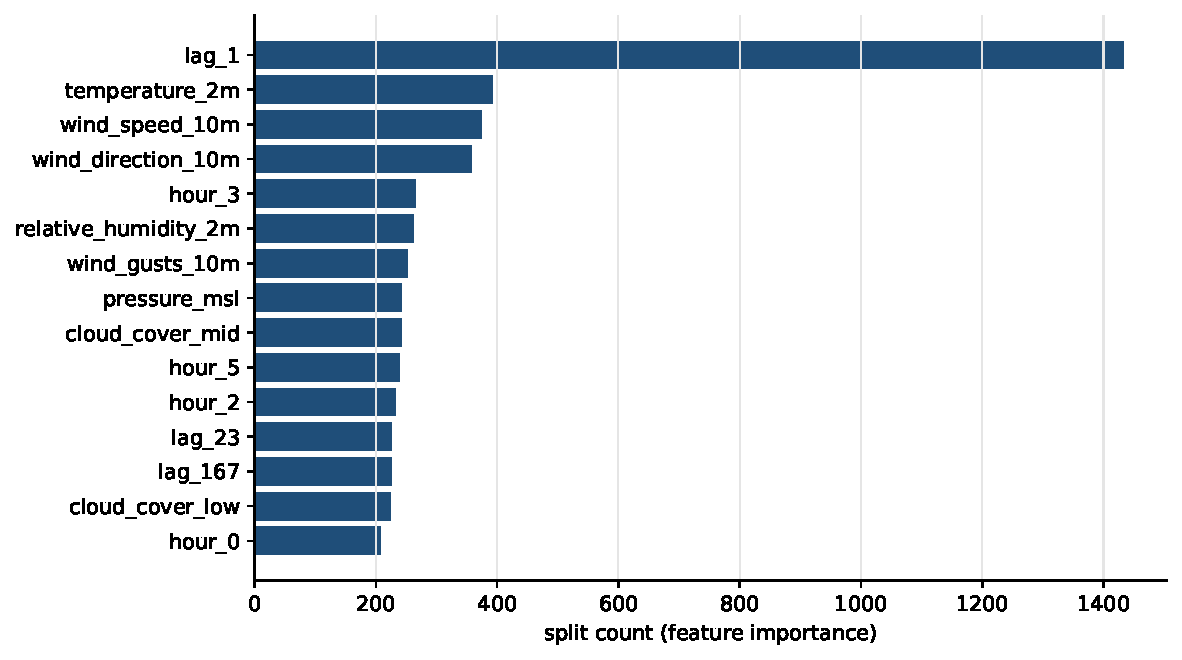
\includegraphics[keepaspectratio]{07_forecaster_training_files/figure-pdf/fig-feature-importance-output-1.pdf}}

}

\caption{\label{fig-feature-importance}Top-15 feature importances of the
trained LightGBM model, measured as `split' frequency over all 400
trees. Lag features (\texttt{lag\_*}) carry the bulk of the information;
weather (temperature) and day-of-week encodings supplement them.}

\end{figure}%

\section{Persist model for follow-up
chapters}\label{persist-model-for-follow-up-chapters}

We store the trained model; chapter 08 reads it back and produces the
24-h forecast.

\protect\phantomsection\label{persist-model}
\begin{Shaded}
\begin{Highlighting}[]
\ImportTok{import}\NormalTok{ pickle}

\NormalTok{model\_path }\OperatorTok{=}\NormalTok{ Path(}\StringTok{"\_cache/forecaster.pkl"}\NormalTok{)}
\ControlFlowTok{with}\NormalTok{ model\_path.}\BuiltInTok{open}\NormalTok{(}\StringTok{"wb"}\NormalTok{) }\ImportTok{as}\NormalTok{ fh:}
\NormalTok{    pickle.dump(model, fh)}
\BuiltInTok{print}\NormalTok{(}\SpecialStringTok{f"Model persisted: }\SpecialCharTok{\{}\NormalTok{model\_path}\SpecialCharTok{\}}\SpecialStringTok{"}\NormalTok{)}
\end{Highlighting}
\end{Shaded}

\begin{verbatim}
Model persisted: _cache/forecaster.pkl
\end{verbatim}

\begin{tcolorbox}[enhanced jigsaw, arc=.35mm, bottomrule=.15mm, bottomtitle=1mm, breakable, colback=white, colbacktitle=quarto-callout-tip-color!10!white, colframe=quarto-callout-tip-color-frame, coltitle=black, left=2mm, leftrule=.75mm, opacityback=0, opacitybacktitle=0.6, rightrule=.15mm, title=\textcolor{quarto-callout-tip-color}{\faLightbulb}\hspace{0.5em}{Exercises (with Claude)}, titlerule=0mm, toprule=.15mm, toptitle=1mm]

\begin{enumerate}
\def\labelenumi{\arabic{enumi}.}
\tightlist
\item
  \emph{CR-4 deny-list.} Ask Claude to display the deny-list of
  forbidden dependencies in \texttt{spotforecast2-safe}'s
  \texttt{pyproject.toml} and to explain for every entry
  (\texttt{plotly}, \texttt{matplotlib}, \texttt{spotoptim},
  \texttt{optuna}, \texttt{torch}, \texttt{tensorflow}) \emph{why} it is
  not admissible in a safety-critical library.
\item
  \emph{Check determinism.} Have Claude write a short function that
  trains the model twice in a row on the same data and compares the
  \texttt{feature\_importances\_} of the two runs bit-by-bit at the end.
  What should come out under correct CR-2 conformance?
\item
  \emph{Hyperparameter awareness.} Discuss with Claude how
  \texttt{lags=24} should qualitatively affect the forecast compared to
  \texttt{lags=168}. Which weekly structure can the model no longer
  learn with only 24 lag hours?
\end{enumerate}

\end{tcolorbox}

\bookmarksetup{startatroot}

\chapter{Produce a 24-hour forecast}\label{sec-forecast}

\begin{tcolorbox}[enhanced jigsaw, arc=.35mm, bottomrule=.15mm, bottomtitle=1mm, breakable, colback=white, colbacktitle=quarto-callout-note-color!10!white, colframe=quarto-callout-note-color-frame, coltitle=black, left=2mm, leftrule=.75mm, opacityback=0, opacitybacktitle=0.6, rightrule=.15mm, title=\textcolor{quarto-callout-note-color}{\faInfo}\hspace{0.5em}{Learning objective}, titlerule=0mm, toprule=.15mm, toptitle=1mm]

You understand the recursive prediction logic and can produce a daily
forecast of the trained forecaster with two lines of code. You see how
that forecast compares to the actual load and to a naive baseline.

\end{tcolorbox}

\section{Recursive multi-step
forecasting}\label{recursive-multi-step-forecasting}

The model was trained to predict \emph{one} hour at a time, given the
last \texttt{lags=168} hours. For a 24-hour daily forecast the
forecaster shifts the 168-hour lag window forward hour by hour:

\[
\hat y_{t+1} = f(y_t, y_{t-1}, \dots, y_{t-167}, \mathbf{x}_{t+1})
\] \[
\hat y_{t+2} = f(\hat y_{t+1}, y_t, \dots, y_{t-166}, \mathbf{x}_{t+2})
\]

At every further step an already predicted value flows into the lag
window. This recursion explains why forecast accuracy typically
deteriorates with the horizon: model errors from earlier hours propagate
to later ones.

\section{AI Act link}\label{ai-act-link-4}

Art. 13 of the AI Act (\emph{transparency and provision of information
to deployers}) demands that a user can understand how the forecast comes
about. By writing the recursion equation out explicitly and making the
lag window visible, we document the mechanism in a way that can be
copied straight into a \texttt{MODEL\_CARD.md}.

\section{Code in action}\label{code-in-action-4}

\protect\phantomsection\label{load-model}
\begin{Shaded}
\begin{Highlighting}[]
\ImportTok{import}\NormalTok{ pandas }\ImportTok{as}\NormalTok{ pd}
\ImportTok{import}\NormalTok{ pickle}
\ImportTok{from}\NormalTok{ pathlib }\ImportTok{import}\NormalTok{ Path}

\NormalTok{shared }\OperatorTok{=}\NormalTok{ Path(}\StringTok{"\_cache/shared"}\NormalTok{)}
\NormalTok{y\_train }\OperatorTok{=}\NormalTok{ pd.read\_parquet(shared }\OperatorTok{/} \StringTok{"y\_train.parquet"}\NormalTok{)[}\StringTok{"load"}\NormalTok{]}
\NormalTok{y\_eval  }\OperatorTok{=}\NormalTok{ pd.read\_parquet(shared }\OperatorTok{/} \StringTok{"y\_eval.parquet"}\NormalTok{)[}\StringTok{"load"}\NormalTok{]}
\NormalTok{exog    }\OperatorTok{=}\NormalTok{ pd.read\_parquet(shared }\OperatorTok{/} \StringTok{"exog.parquet"}\NormalTok{)}

\ControlFlowTok{with}\NormalTok{ Path(}\StringTok{"\_cache/forecaster.pkl"}\NormalTok{).}\BuiltInTok{open}\NormalTok{(}\StringTok{"rb"}\NormalTok{) }\ImportTok{as}\NormalTok{ fh:}
\NormalTok{    model }\OperatorTok{=}\NormalTok{ pickle.load(fh)}
\end{Highlighting}
\end{Shaded}

We hand the forecaster the last lag window \emph{explicitly}. For the
model with \texttt{lags=168} those are the last 168 hours of the
training range. That way you see immediately which past information
enters the first forecast hour.

\protect\phantomsection\label{predict-24h}
\begin{Shaded}
\begin{Highlighting}[]
\NormalTok{y\_eval\_24h }\OperatorTok{=}\NormalTok{ y\_eval.iloc[:}\DecValTok{24}\NormalTok{]}
\NormalTok{last\_window }\OperatorTok{=}\NormalTok{ y\_train.iloc[}\OperatorTok{{-}}\DecValTok{168}\NormalTok{:].copy()}
\CommentTok{\# A parquet round{-}trip loses the \textasciigrave{}freq\textasciigrave{} attribute of the DatetimeIndex.}
\CommentTok{\# The forecaster needs it to construct the prediction index:}
\NormalTok{last\_window.index }\OperatorTok{=}\NormalTok{ pd.DatetimeIndex(last\_window.index, freq}\OperatorTok{=}\StringTok{"h"}\NormalTok{)}

\NormalTok{y\_pred }\OperatorTok{=}\NormalTok{ model.forecaster.predict(}
\NormalTok{    steps}\OperatorTok{=}\DecValTok{24}\NormalTok{,}
\NormalTok{    last\_window}\OperatorTok{=}\NormalTok{last\_window,}
\NormalTok{    exog}\OperatorTok{=}\NormalTok{exog.loc[y\_eval\_24h.index],}
\NormalTok{)}
\NormalTok{y\_pred.name }\OperatorTok{=} \StringTok{"forecast"}
\NormalTok{y\_pred.index }\OperatorTok{=}\NormalTok{ y\_eval\_24h.index}

\BuiltInTok{print}\NormalTok{(}\SpecialStringTok{f"Forecast produced: }\SpecialCharTok{\{}\BuiltInTok{len}\NormalTok{(y\_pred)}\SpecialCharTok{\}}\SpecialStringTok{ hours, "}
      \SpecialStringTok{f"}\SpecialCharTok{\{}\NormalTok{y\_pred}\SpecialCharTok{.}\NormalTok{index[}\DecValTok{0}\NormalTok{]}\SpecialCharTok{\}}\SpecialStringTok{ ... }\SpecialCharTok{\{}\NormalTok{y\_pred}\SpecialCharTok{.}\NormalTok{index[}\OperatorTok{{-}}\DecValTok{1}\NormalTok{]}\SpecialCharTok{\}}\SpecialStringTok{"}\NormalTok{)}
\BuiltInTok{print}\NormalTok{(}\SpecialStringTok{f"Last lag hour:    }\SpecialCharTok{\{}\NormalTok{last\_window}\SpecialCharTok{.}\NormalTok{index[}\OperatorTok{{-}}\DecValTok{1}\NormalTok{]}\SpecialCharTok{\}}\SpecialStringTok{"}\NormalTok{)}
\BuiltInTok{print}\NormalTok{(}\StringTok{"First three forecast hours:"}\NormalTok{)}
\BuiltInTok{print}\NormalTok{(y\_pred.head(}\DecValTok{3}\NormalTok{).}\BuiltInTok{round}\NormalTok{(}\DecValTok{1}\NormalTok{).to\_string())}
\end{Highlighting}
\end{Shaded}

\begin{verbatim}
Forecast produced: 24 hours, 2024-11-01 00:00:00+00:00 ... 2024-11-01 23:00:00+00:00
Last lag hour:    2024-10-31 23:00:00+00:00
First three forecast hours:
Time (UTC)
2024-11-01 00:00:00+00:00    42052.3
2024-11-01 01:00:00+00:00    41891.0
2024-11-01 02:00:00+00:00    42106.2
\end{verbatim}

\section{Visualisation: forecast, reality,
baseline}\label{visualisation-forecast-reality-baseline}

A forecast deserves the name only when it is \emph{better} than a
trivial baseline. We take \emph{weekly persistence} as a baseline: the
load of the same hour seven days earlier. If our model does not clearly
beat this baseline, the whole effort was in vain.

\begin{Shaded}
\begin{Highlighting}[]
\ImportTok{import}\NormalTok{ matplotlib.pyplot }\ImportTok{as}\NormalTok{ plt}
\ImportTok{import}\NormalTok{ matplotlib.dates }\ImportTok{as}\NormalTok{ mdates}

\NormalTok{train\_tail }\OperatorTok{=}\NormalTok{ y\_train.iloc[}\OperatorTok{{-}}\DecValTok{24}\NormalTok{:]}
\NormalTok{y\_clean }\OperatorTok{=}\NormalTok{ pd.read\_parquet(shared }\OperatorTok{/} \StringTok{"load\_de\_2024\_clean.parquet"}\NormalTok{)[}\StringTok{"load"}\NormalTok{]}
\NormalTok{persistence }\OperatorTok{=}\NormalTok{ y\_clean.shift(}\DecValTok{168}\NormalTok{).loc[y\_eval\_24h.index]}

\NormalTok{fig, ax }\OperatorTok{=}\NormalTok{ plt.subplots(figsize}\OperatorTok{=}\NormalTok{(}\FloatTok{8.5}\NormalTok{, }\FloatTok{3.5}\NormalTok{))}
\NormalTok{ax.plot(train\_tail.index, train\_tail.values }\OperatorTok{/} \DecValTok{1000}\NormalTok{,}
\NormalTok{        color}\OperatorTok{=}\StringTok{"\#1F4E79"}\NormalTok{, linewidth}\OperatorTok{=}\FloatTok{1.0}\NormalTok{, label}\OperatorTok{=}\StringTok{"Training (tail)"}\NormalTok{)}
\NormalTok{ax.plot(y\_eval\_24h.index, y\_eval\_24h.values }\OperatorTok{/} \DecValTok{1000}\NormalTok{,}
\NormalTok{        color}\OperatorTok{=}\StringTok{"\#1F4E79"}\NormalTok{, linewidth}\OperatorTok{=}\FloatTok{1.0}\NormalTok{, linestyle}\OperatorTok{=}\StringTok{":"}\NormalTok{)}
\NormalTok{ax.plot(y\_pred.index, y\_pred.values }\OperatorTok{/} \DecValTok{1000}\NormalTok{,}
\NormalTok{        color}\OperatorTok{=}\StringTok{"\#2E7D55"}\NormalTok{, linewidth}\OperatorTok{=}\FloatTok{1.4}\NormalTok{, label}\OperatorTok{=}\StringTok{"Model forecast"}\NormalTok{)}
\NormalTok{ax.plot(y\_eval\_24h.index, y\_eval\_24h.values }\OperatorTok{/} \DecValTok{1000}\NormalTok{,}
\NormalTok{        color}\OperatorTok{=}\StringTok{"\#E07B00"}\NormalTok{, linewidth}\OperatorTok{=}\FloatTok{1.0}\NormalTok{, label}\OperatorTok{=}\StringTok{"observed (evaluation)"}\NormalTok{)}
\NormalTok{ax.plot(persistence.index, persistence.values }\OperatorTok{/} \DecValTok{1000}\NormalTok{,}
\NormalTok{        color}\OperatorTok{=}\StringTok{"\#8E63B5"}\NormalTok{, linewidth}\OperatorTok{=}\FloatTok{1.0}\NormalTok{, linestyle}\OperatorTok{=}\StringTok{"{-}{-}"}\NormalTok{, label}\OperatorTok{=}\StringTok{"Weekly persistence"}\NormalTok{)}

\NormalTok{split }\OperatorTok{=}\NormalTok{ train\_tail.index[}\OperatorTok{{-}}\DecValTok{1}\NormalTok{] }\OperatorTok{+}\NormalTok{ pd.Timedelta(hours}\OperatorTok{=}\DecValTok{1}\NormalTok{)}
\NormalTok{ax.axvline(split, color}\OperatorTok{=}\StringTok{"\#555555"}\NormalTok{, linestyle}\OperatorTok{=}\StringTok{"{-}{-}"}\NormalTok{, linewidth}\OperatorTok{=}\FloatTok{0.7}\NormalTok{)}
\NormalTok{ax.text(split, ax.get\_ylim()[}\DecValTok{1}\NormalTok{], }\StringTok{"  End of training"}\NormalTok{,}
\NormalTok{        ha}\OperatorTok{=}\StringTok{"left"}\NormalTok{, va}\OperatorTok{=}\StringTok{"top"}\NormalTok{, fontsize}\OperatorTok{=}\DecValTok{8}\NormalTok{, color}\OperatorTok{=}\StringTok{"\#555555"}\NormalTok{)}

\NormalTok{ax.set\_ylabel(}\StringTok{"Load [GW]"}\NormalTok{)}
\NormalTok{ax.set\_xlabel(}\StringTok{"Time"}\NormalTok{)}
\NormalTok{ax.grid(}\VariableTok{True}\NormalTok{, color}\OperatorTok{=}\StringTok{"\#E5E5E5"}\NormalTok{, linewidth}\OperatorTok{=}\FloatTok{0.5}\NormalTok{)}
\NormalTok{ax.xaxis.set\_major\_locator(mdates.HourLocator(byhour}\OperatorTok{=}\NormalTok{[}\DecValTok{0}\NormalTok{, }\DecValTok{12}\NormalTok{]))}
\NormalTok{ax.xaxis.set\_major\_formatter(mdates.DateFormatter(}\StringTok{"}\SpecialCharTok{\%{-}d}\StringTok{.\%{-}m \%H:\%M"}\NormalTok{))}
\NormalTok{ax.legend(loc}\OperatorTok{=}\StringTok{"upper left"}\NormalTok{, frameon}\OperatorTok{=}\VariableTok{False}\NormalTok{, fontsize}\OperatorTok{=}\DecValTok{8}\NormalTok{)}
\ControlFlowTok{for}\NormalTok{ s }\KeywordTok{in}\NormalTok{ (}\StringTok{"top"}\NormalTok{, }\StringTok{"right"}\NormalTok{):}
\NormalTok{    ax.spines[s].set\_visible(}\VariableTok{False}\NormalTok{)}
\NormalTok{fig.tight\_layout()}
\NormalTok{plt.show()}
\end{Highlighting}
\end{Shaded}

\begin{figure}[H]

\centering{

\pandocbounded{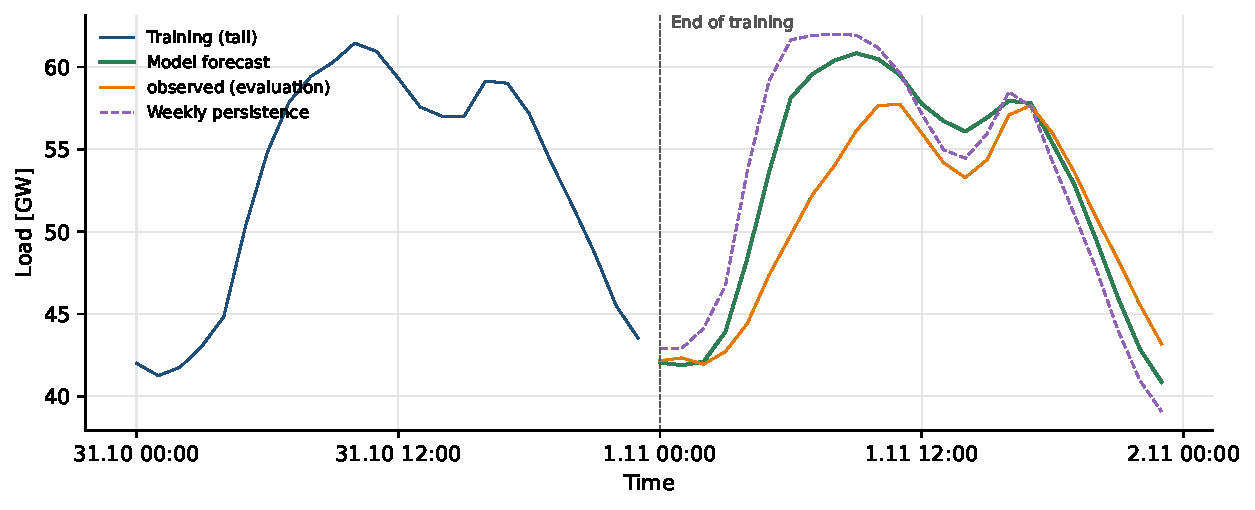
\includegraphics[keepaspectratio]{08_forecast_files/figure-pdf/fig-forecast-vs-actual-output-1.pdf}}

}

\caption{\label{fig-forecast-vs-actual}Comparison of the 24-hour
forecast with the actual load and the weekly-persistence baseline (load
seven days earlier, same hour). The window covers the last 24 training
hours plus the first 24 evaluation hours. The vertical dashed line marks
the end of the training period.}

\end{figure}%

\section{Persisting for follow-up
chapters}\label{persisting-for-follow-up-chapters-2}

\protect\phantomsection\label{persist-pred}
\begin{Shaded}
\begin{Highlighting}[]
\NormalTok{y\_pred.to\_frame(}\StringTok{"forecast"}\NormalTok{).to\_parquet(shared }\OperatorTok{/} \StringTok{"y\_pred\_24h.parquet"}\NormalTok{)}
\end{Highlighting}
\end{Shaded}

\begin{tcolorbox}[enhanced jigsaw, arc=.35mm, bottomrule=.15mm, bottomtitle=1mm, breakable, colback=white, colbacktitle=quarto-callout-tip-color!10!white, colframe=quarto-callout-tip-color-frame, coltitle=black, left=2mm, leftrule=.75mm, opacityback=0, opacitybacktitle=0.6, rightrule=.15mm, title=\textcolor{quarto-callout-tip-color}{\faLightbulb}\hspace{0.5em}{Exercises (with Claude)}, titlerule=0mm, toprule=.15mm, toptitle=1mm]

\begin{enumerate}
\def\labelenumi{\arabic{enumi}.}
\tightlist
\item
  \emph{Understand recursion error.} Have Claude rebuild the recursion
  equation by hand in a small loop (with a trivial model such as
  \texttt{f(y,\ x)\ =\ mean(y{[}-24:{]})}) and demonstrate on a 96-hour
  horizon how model errors amplify over time.
\item
  \emph{Change the lag window.} Discuss with Claude what happens when
  you predict \texttt{steps=72} (3 days) instead of \texttt{steps=24}.
  Which hours among the last 24 predictions are probably the least
  accurate and why?
\item
  \emph{Transparency for the deployer.} Ask Claude to write an example
  entry for a \texttt{MODEL\_CARD.md} that explains \emph{recursive
  forecasting} to a non-technical reader in three sentences and spells
  out what consequence this has for the forecast uncertainty at the end
  of the horizon.
\end{enumerate}

\end{tcolorbox}

\bookmarksetup{startatroot}

\chapter{Measuring accuracy: MAE, MSE, RMSE, MAPE}\label{sec-accuracy}

\begin{tcolorbox}[enhanced jigsaw, arc=.35mm, bottomrule=.15mm, bottomtitle=1mm, breakable, colback=white, colbacktitle=quarto-callout-note-color!10!white, colframe=quarto-callout-note-color-frame, coltitle=black, left=2mm, leftrule=.75mm, opacityback=0, opacitybacktitle=0.6, rightrule=.15mm, title=\textcolor{quarto-callout-note-color}{\faInfo}\hspace{0.5em}{Learning objective}, titlerule=0mm, toprule=.15mm, toptitle=1mm]

You can compute the four standard measures of point-forecast accuracy,
explain their geometric meaning, and distinguish \emph{which} measure is
appropriate for a given risk question.

\end{tcolorbox}

\section{Why four measures instead of
one?}\label{why-four-measures-instead-of-one}

A load forecast can go wrong in many ways: many small errors in one
direction, a single huge outlier, a consistent upward or downward
offset. No single measure summarises all of that. We therefore look at
four:

\begin{itemize}
\tightlist
\item
  \emph{Mean Absolute Error} (MAE): the average deviation in load units.
  Robust, easy to interpret, treats one large and many small errors with
  equal weight.
\item
  \emph{Mean Squared Error} (MSE): the average squared deviation.
  Penalises large outliers disproportionately. Has units of ``load
  squared''.
\item
  \emph{Root Mean Squared Error} (RMSE): square root of the MSE; again
  in load units, but with outlier sensitivity.
\item
  \emph{Mean Absolute Percentage Error} (MAPE): the average deviation in
  per cent. Allows comparisons between different load levels.
\end{itemize}

\section{AI Act link}\label{ai-act-link-5}

Art. 15 of the AI Act (\emph{accuracy, robustness and cybersecurity})
demands that high-risk AI systems achieve ``appropriate levels of
accuracy'' and declare those in the \texttt{MODEL\_CARD.md}. What is
``appropriate'' depends on the use case. For a daily forecast of the
electric load, a MAPE below 4\% would be considered state of the art.

\section{Code in action}\label{code-in-action-5}

\protect\phantomsection\label{load-and-measure}
\begin{Shaded}
\begin{Highlighting}[]
\ImportTok{import}\NormalTok{ numpy }\ImportTok{as}\NormalTok{ np}
\ImportTok{import}\NormalTok{ pandas }\ImportTok{as}\NormalTok{ pd}
\ImportTok{from}\NormalTok{ pathlib }\ImportTok{import}\NormalTok{ Path}
\ImportTok{from}\NormalTok{ spotforecast2\_safe.manager.demo\_metrics }\ImportTok{import}\NormalTok{ calculate\_metrics}

\NormalTok{shared }\OperatorTok{=}\NormalTok{ Path(}\StringTok{"\_cache/shared"}\NormalTok{)}
\NormalTok{y\_eval }\OperatorTok{=}\NormalTok{ pd.read\_parquet(shared }\OperatorTok{/} \StringTok{"y\_eval.parquet"}\NormalTok{)[}\StringTok{"load"}\NormalTok{]}
\NormalTok{y\_pred }\OperatorTok{=}\NormalTok{ pd.read\_parquet(shared }\OperatorTok{/} \StringTok{"y\_pred\_24h.parquet"}\NormalTok{)[}\StringTok{"forecast"}\NormalTok{]}
\NormalTok{y\_eval\_24h }\OperatorTok{=}\NormalTok{ y\_eval.iloc[:}\DecValTok{24}\NormalTok{]}

\NormalTok{m }\OperatorTok{=}\NormalTok{ calculate\_metrics(actual}\OperatorTok{=}\NormalTok{y\_eval\_24h, predicted}\OperatorTok{=}\NormalTok{y\_pred)}
\NormalTok{mae  }\OperatorTok{=} \BuiltInTok{float}\NormalTok{(m[}\StringTok{"MAE"}\NormalTok{])}
\NormalTok{mse  }\OperatorTok{=} \BuiltInTok{float}\NormalTok{(m[}\StringTok{"MSE"}\NormalTok{])}
\NormalTok{rmse }\OperatorTok{=} \BuiltInTok{float}\NormalTok{(np.sqrt(mse))}
\NormalTok{mape }\OperatorTok{=} \BuiltInTok{float}\NormalTok{(np.mean(np.}\BuiltInTok{abs}\NormalTok{((y\_eval\_24h.values }\OperatorTok{{-}}\NormalTok{ y\_pred.values) }\OperatorTok{/}\NormalTok{ y\_eval\_24h.values)))}

\BuiltInTok{print}\NormalTok{(}\SpecialStringTok{f"MAE  = }\SpecialCharTok{\{}\NormalTok{mae}\SpecialCharTok{:7.1f\}}\SpecialStringTok{   MW   (mean absolute error)"}\NormalTok{)}
\BuiltInTok{print}\NormalTok{(}\SpecialStringTok{f"MSE  = }\SpecialCharTok{\{}\NormalTok{mse}\SpecialCharTok{:9.1f\}}\SpecialStringTok{   MW\^{}2 (mean squared error)"}\NormalTok{)}
\BuiltInTok{print}\NormalTok{(}\SpecialStringTok{f"RMSE = }\SpecialCharTok{\{}\NormalTok{rmse}\SpecialCharTok{:7.1f\}}\SpecialStringTok{   MW   (root mean squared error)"}\NormalTok{)}
\BuiltInTok{print}\NormalTok{(}\SpecialStringTok{f"MAPE = }\SpecialCharTok{\{}\NormalTok{mape}\SpecialCharTok{:7.2\%\}}\SpecialStringTok{        (mean absolute percentage error)"}\NormalTok{)}
\end{Highlighting}
\end{Shaded}

\begin{verbatim}
MAE  =  2673.4   MW   (mean absolute error)
MSE  = 12446842.1   MW^2 (mean squared error)
RMSE =  3528.0   MW   (root mean squared error)
MAPE =   5.26%        (mean absolute percentage error)
\end{verbatim}

\section{Visualisation: geometry of the
metrics}\label{visualisation-geometry-of-the-metrics}

An evocative view of the measures: the \emph{histogram of residuals}
(forecast minus actual value). The MAE is the average distance from
zero; the RMSE is the spread weighted by error size. Both can be drawn
as vertical lines.

\begin{Shaded}
\begin{Highlighting}[]
\ImportTok{import}\NormalTok{ matplotlib.pyplot }\ImportTok{as}\NormalTok{ plt}

\NormalTok{residuals }\OperatorTok{=}\NormalTok{ (y\_pred.values }\OperatorTok{{-}}\NormalTok{ y\_eval\_24h.values) }\OperatorTok{/} \DecValTok{1000}  \CommentTok{\# in GW}

\NormalTok{fig, ax }\OperatorTok{=}\NormalTok{ plt.subplots(figsize}\OperatorTok{=}\NormalTok{(}\FloatTok{8.5}\NormalTok{, }\FloatTok{3.5}\NormalTok{))}
\NormalTok{ax.hist(residuals, bins}\OperatorTok{=}\DecValTok{12}\NormalTok{, color}\OperatorTok{=}\StringTok{"\#1F4E79"}\NormalTok{, alpha}\OperatorTok{=}\FloatTok{0.85}\NormalTok{, edgecolor}\OperatorTok{=}\StringTok{"white"}\NormalTok{)}
\NormalTok{ax.axvline(}\DecValTok{0}\NormalTok{, color}\OperatorTok{=}\StringTok{"\#000000"}\NormalTok{, linewidth}\OperatorTok{=}\FloatTok{0.8}\NormalTok{)}
\NormalTok{ax.axvline(}\OperatorTok{+}\NormalTok{mae }\OperatorTok{/} \DecValTok{1000}\NormalTok{, color}\OperatorTok{=}\StringTok{"\#E07B00"}\NormalTok{, linestyle}\OperatorTok{=}\StringTok{"{-}{-}"}\NormalTok{, linewidth}\OperatorTok{=}\FloatTok{1.2}\NormalTok{, label}\OperatorTok{=}\SpecialStringTok{f"+MAE = }\SpecialCharTok{\{}\NormalTok{mae}\OperatorTok{/}\DecValTok{1000}\SpecialCharTok{:.2f\}}\SpecialStringTok{ GW"}\NormalTok{)}
\NormalTok{ax.axvline(}\OperatorTok{{-}}\NormalTok{mae }\OperatorTok{/} \DecValTok{1000}\NormalTok{, color}\OperatorTok{=}\StringTok{"\#E07B00"}\NormalTok{, linestyle}\OperatorTok{=}\StringTok{"{-}{-}"}\NormalTok{, linewidth}\OperatorTok{=}\FloatTok{1.2}\NormalTok{)}
\NormalTok{ax.axvline(}\OperatorTok{+}\NormalTok{rmse }\OperatorTok{/} \DecValTok{1000}\NormalTok{, color}\OperatorTok{=}\StringTok{"\#2E7D55"}\NormalTok{, linestyle}\OperatorTok{=}\StringTok{":"}\NormalTok{, linewidth}\OperatorTok{=}\FloatTok{1.2}\NormalTok{, label}\OperatorTok{=}\SpecialStringTok{f"+RMSE = }\SpecialCharTok{\{}\NormalTok{rmse}\OperatorTok{/}\DecValTok{1000}\SpecialCharTok{:.2f\}}\SpecialStringTok{ GW"}\NormalTok{)}
\NormalTok{ax.axvline(}\OperatorTok{{-}}\NormalTok{rmse }\OperatorTok{/} \DecValTok{1000}\NormalTok{, color}\OperatorTok{=}\StringTok{"\#2E7D55"}\NormalTok{, linestyle}\OperatorTok{=}\StringTok{":"}\NormalTok{, linewidth}\OperatorTok{=}\FloatTok{1.2}\NormalTok{)}
\NormalTok{ax.set\_xlabel(}\StringTok{"Residual (forecast {-} observed) [GW]"}\NormalTok{)}
\NormalTok{ax.set\_ylabel(}\StringTok{"Number of hours"}\NormalTok{)}
\NormalTok{ax.legend(loc}\OperatorTok{=}\StringTok{"upper right"}\NormalTok{, frameon}\OperatorTok{=}\VariableTok{False}\NormalTok{)}
\NormalTok{ax.grid(}\VariableTok{True}\NormalTok{, color}\OperatorTok{=}\StringTok{"\#E5E5E5"}\NormalTok{, linewidth}\OperatorTok{=}\FloatTok{0.5}\NormalTok{)}
\ControlFlowTok{for}\NormalTok{ s }\KeywordTok{in}\NormalTok{ (}\StringTok{"top"}\NormalTok{, }\StringTok{"right"}\NormalTok{):}
\NormalTok{    ax.spines[s].set\_visible(}\VariableTok{False}\NormalTok{)}
\NormalTok{fig.tight\_layout()}
\NormalTok{plt.show()}
\end{Highlighting}
\end{Shaded}

\begin{figure}[H]

\centering{

\pandocbounded{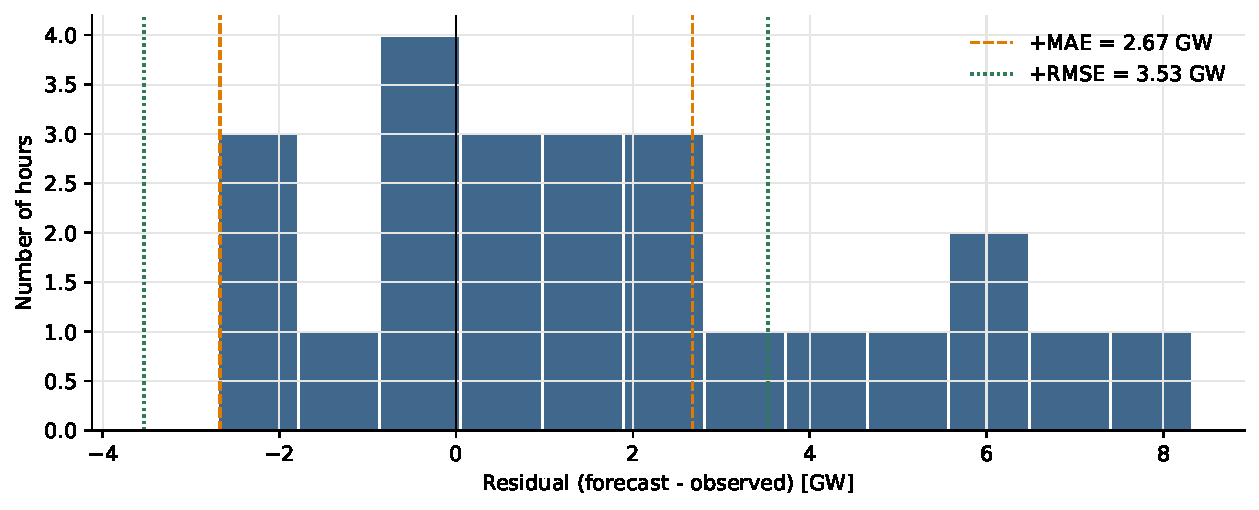
\includegraphics[keepaspectratio]{09_accuracy_files/figure-pdf/fig-metrics-geometry-output-1.pdf}}

}

\caption{\label{fig-metrics-geometry}Histogram of the 24 residuals of
the daily forecast. The vertical lines show MAE and RMSE as alternative
spread measures. Here the MAE is the average of the absolute distances
to zero; the RMSE is the square root of the average of the squared
distances and is influenced more strongly by the outlier at the
histogram edge.}

\end{figure}%

\section{When is which measure
appropriate?}\label{when-is-which-measure-appropriate}

{\def\LTcaptype{none} % do not increment counter
\begin{longtable}[]{@{}
  >{\raggedright\arraybackslash}p{(\linewidth - 2\tabcolsep) * \real{0.7465}}
  >{\raggedright\arraybackslash}p{(\linewidth - 2\tabcolsep) * \real{0.2535}}@{}}
\toprule\noalign{}
\begin{minipage}[b]{\linewidth}\raggedright
Question
\end{minipage} & \begin{minipage}[b]{\linewidth}\raggedright
Suitable measure
\end{minipage} \\
\midrule\noalign{}
\endhead
\bottomrule\noalign{}
\endlastfoot
How much reserve energy do I need to plan in bulk? & MAE \\
How severe are the rare large errors? & RMSE or MSE \\
How does my system compare to one in another market zone? & MAPE \\
Which component of my risk capital is sufficient? & RMSE plus a quantile
bound \\
\end{longtable}
}

\section{Comparison with the
baseline}\label{comparison-with-the-baseline}

Without comparison to a trivial baseline an accuracy number is
meaningless. We compute the same measures for the weekly persistence:

\protect\phantomsection\label{baseline-metrics}
\begin{Shaded}
\begin{Highlighting}[]
\NormalTok{y\_clean }\OperatorTok{=}\NormalTok{ pd.read\_parquet(shared }\OperatorTok{/} \StringTok{"load\_de\_2024\_clean.parquet"}\NormalTok{)[}\StringTok{"load"}\NormalTok{]}
\NormalTok{persistence }\OperatorTok{=}\NormalTok{ y\_clean.shift(}\DecValTok{168}\NormalTok{).loc[y\_eval\_24h.index]}

\NormalTok{mae\_p  }\OperatorTok{=} \BuiltInTok{float}\NormalTok{((y\_eval\_24h.values }\OperatorTok{{-}}\NormalTok{ persistence.values).}\FunctionTok{\_\_abs\_\_}\NormalTok{().mean())}
\NormalTok{mape\_p }\OperatorTok{=} \BuiltInTok{float}\NormalTok{(np.mean(np.}\BuiltInTok{abs}\NormalTok{((y\_eval\_24h.values }\OperatorTok{{-}}\NormalTok{ persistence.values) }\OperatorTok{/}\NormalTok{ y\_eval\_24h.values)))}

\BuiltInTok{print}\NormalTok{(}\SpecialStringTok{f"            Model       Weekly persistence"}\NormalTok{)}
\BuiltInTok{print}\NormalTok{(}\SpecialStringTok{f"MAE    }\SpecialCharTok{\{}\NormalTok{mae}\SpecialCharTok{:8.1f\}}\SpecialStringTok{ MW    }\SpecialCharTok{\{}\NormalTok{mae\_p}\SpecialCharTok{:8.1f\}}\SpecialStringTok{ MW"}\NormalTok{)}
\BuiltInTok{print}\NormalTok{(}\SpecialStringTok{f"MAPE   }\SpecialCharTok{\{}\NormalTok{mape}\SpecialCharTok{:8.2\%\}}\SpecialStringTok{      }\SpecialCharTok{\{}\NormalTok{mape\_p}\SpecialCharTok{:8.2\%\}}\SpecialStringTok{"}\NormalTok{)}
\end{Highlighting}
\end{Shaded}

\begin{verbatim}
            Model       Weekly persistence
MAE      2673.4 MW      3995.0 MW
MAPE      5.26%         8.08%
\end{verbatim}

\begin{tcolorbox}[enhanced jigsaw, arc=.35mm, bottomrule=.15mm, bottomtitle=1mm, breakable, colback=white, colbacktitle=quarto-callout-tip-color!10!white, colframe=quarto-callout-tip-color-frame, coltitle=black, left=2mm, leftrule=.75mm, opacityback=0, opacitybacktitle=0.6, rightrule=.15mm, title=\textcolor{quarto-callout-tip-color}{\faLightbulb}\hspace{0.5em}{Exercises (with Claude)}, titlerule=0mm, toprule=.15mm, toptitle=1mm]

\begin{enumerate}
\def\labelenumi{\arabic{enumi}.}
\tightlist
\item
  \emph{Choosing measures.} Discuss with Claude a concrete use case
  (``We need the forecast in order to prepare our reserve gas-fired
  plants tomorrow at 06:00'') and have it argue which of the four
  measures the transmission system operator should include as a KPI in
  its \texttt{MODEL\_CARD.md}.
\item
  \emph{Own implementation.} Ask Claude to program the four measures by
  hand with \texttt{numpy}, without \texttt{calculate\_metrics}, and
  compare them with the library function. What happens when a single
  actual value is zero (division by zero in MAPE)?
\item
  \emph{Robustness to outliers.} Have Claude generate a synthetic 24-h
  vector in which 23 values are very accurate (error \(\pm\) 50 MW) and
  a single value is far off (\(\pm\) 5000 MW). How do MAE and RMSE
  behave? Which measure shows the ``problem'' more clearly?
\end{enumerate}

\end{tcolorbox}

\bookmarksetup{startatroot}

\chapter{Rolling-origin backtest}\label{sec-backtest}

\begin{tcolorbox}[enhanced jigsaw, arc=.35mm, bottomrule=.15mm, bottomtitle=1mm, breakable, colback=white, colbacktitle=quarto-callout-note-color!10!white, colframe=quarto-callout-note-color-frame, coltitle=black, left=2mm, leftrule=.75mm, opacityback=0, opacitybacktitle=0.6, rightrule=.15mm, title=\textcolor{quarto-callout-note-color}{\faInfo}\hspace{0.5em}{Learning objective}, titlerule=0mm, toprule=.15mm, toptitle=1mm]

You understand why a single train/test split does not yield a robust
accuracy verdict, and you can set up a rolling-origin backtest with
\texttt{TimeSeriesFold} that estimates the forecast quality over several
weeks.

\end{tcolorbox}

\section{Why backtest at all?}\label{why-backtest-at-all}

In the previous chapter we forecast the first 24 hours of the evaluation
range and measured three accuracy metrics on it. What if those very 24
hours are unusually good --- or unusually bad? A single measurement at a
single point on the time axis is \emph{not} a robust verdict on the
model quality.

A \emph{rolling-origin backtest} shifts the forecast start point step by
step through the entire evaluation period and runs a 24-hour forecast at
each step. The result is a whole distribution of accuracy measurements:
you see not only the mean but also the spread; not only the best- and
worst-case but the typical range of variation.

\section{AI Act link}\label{ai-act-link-6}

Art. 9 of the AI Act (\emph{risk management}) demands a \emph{testing}
of the system before it is put into service. Art. 10(3) requires that
validation datasets are ``representative'' --- a term that, without an
empirical test, remains a mere claim. The backtest provides exactly that
empirical test.

\section{Code in action}\label{code-in-action-6}

\protect\phantomsection\label{load-state-bt}
\begin{Shaded}
\begin{Highlighting}[]
\ImportTok{import}\NormalTok{ pandas }\ImportTok{as}\NormalTok{ pd}
\ImportTok{import}\NormalTok{ pickle}
\ImportTok{from}\NormalTok{ pathlib }\ImportTok{import}\NormalTok{ Path}

\NormalTok{shared }\OperatorTok{=}\NormalTok{ Path(}\StringTok{"\_cache/shared"}\NormalTok{)}
\NormalTok{y\_clean }\OperatorTok{=}\NormalTok{ pd.read\_parquet(shared }\OperatorTok{/} \StringTok{"load\_de\_2024\_clean.parquet"}\NormalTok{)[}\StringTok{"load"}\NormalTok{]}
\NormalTok{y\_train }\OperatorTok{=}\NormalTok{ pd.read\_parquet(shared }\OperatorTok{/} \StringTok{"y\_train.parquet"}\NormalTok{)[}\StringTok{"load"}\NormalTok{]}
\NormalTok{exog    }\OperatorTok{=}\NormalTok{ pd.read\_parquet(shared }\OperatorTok{/} \StringTok{"exog.parquet"}\NormalTok{)}

\CommentTok{\# A parquet round{-}trip drops the \textasciigrave{}freq\textasciigrave{} attribute of the DatetimeIndices;}
\CommentTok{\# the forecaster needs it to construct forecast indices.}
\NormalTok{y\_clean.index }\OperatorTok{=}\NormalTok{ pd.DatetimeIndex(y\_clean.index, freq}\OperatorTok{=}\StringTok{"h"}\NormalTok{)}
\NormalTok{y\_train.index }\OperatorTok{=}\NormalTok{ pd.DatetimeIndex(y\_train.index, freq}\OperatorTok{=}\StringTok{"h"}\NormalTok{)}
\NormalTok{exog.index    }\OperatorTok{=}\NormalTok{ pd.DatetimeIndex(exog.index, freq}\OperatorTok{=}\StringTok{"h"}\NormalTok{)}

\ControlFlowTok{with}\NormalTok{ Path(}\StringTok{"\_cache/forecaster.pkl"}\NormalTok{).}\BuiltInTok{open}\NormalTok{(}\StringTok{"rb"}\NormalTok{) }\ImportTok{as}\NormalTok{ fh:}
\NormalTok{    model }\OperatorTok{=}\NormalTok{ pickle.load(fh)}
\end{Highlighting}
\end{Shaded}

\protect\phantomsection\label{run-backtest}
\begin{Shaded}
\begin{Highlighting}[]
\ImportTok{from}\NormalTok{ spotforecast2\_safe.backtesting.validation }\ImportTok{import}\NormalTok{ (}
\NormalTok{    TimeSeriesFold, backtesting\_forecaster}
\NormalTok{)}

\CommentTok{\# We restrict the backtest to the range for which calendar and weather}
\CommentTok{\# features are available (training + evaluation range from chapter 05).}
\CommentTok{\# That way we avoid asking the forecaster for hours whose \textasciigrave{}exog\textasciigrave{} values}
\CommentTok{\# do not exist.}
\NormalTok{y\_bt }\OperatorTok{=}\NormalTok{ y\_clean.loc[exog.index.}\BuiltInTok{min}\NormalTok{():exog.index.}\BuiltInTok{max}\NormalTok{()]}

\NormalTok{cv }\OperatorTok{=}\NormalTok{ TimeSeriesFold(}
\NormalTok{    steps}\OperatorTok{=}\DecValTok{24}\NormalTok{,}
\NormalTok{    initial\_train\_size}\OperatorTok{=}\BuiltInTok{len}\NormalTok{(y\_train),}
\NormalTok{    refit}\OperatorTok{=}\VariableTok{False}\NormalTok{,}
\NormalTok{    fixed\_train\_size}\OperatorTok{=}\VariableTok{False}\NormalTok{,}
\NormalTok{    verbose}\OperatorTok{=}\VariableTok{False}\NormalTok{,}
\NormalTok{)}

\NormalTok{metrics\_df, predictions\_df }\OperatorTok{=}\NormalTok{ backtesting\_forecaster(}
\NormalTok{    forecaster}\OperatorTok{=}\NormalTok{model.forecaster,}
\NormalTok{    y}\OperatorTok{=}\NormalTok{y\_bt,}
\NormalTok{    cv}\OperatorTok{=}\NormalTok{cv,}
\NormalTok{    metric}\OperatorTok{=}\StringTok{"mean\_absolute\_error"}\NormalTok{,}
\NormalTok{    exog}\OperatorTok{=}\NormalTok{exog,}
\NormalTok{    show\_progress}\OperatorTok{=}\VariableTok{False}\NormalTok{,}
\NormalTok{    verbose}\OperatorTok{=}\VariableTok{False}\NormalTok{,}
\NormalTok{)}
\BuiltInTok{print}\NormalTok{(}\SpecialStringTok{f"Number of folds:    }\SpecialCharTok{\{}\BuiltInTok{len}\NormalTok{(metrics\_df)}\SpecialCharTok{\}}\SpecialStringTok{"}\NormalTok{)}
\BuiltInTok{print}\NormalTok{(}\SpecialStringTok{f"Mean MAE:           }\SpecialCharTok{\{}\BuiltInTok{float}\NormalTok{(metrics\_df.iloc[}\DecValTok{0}\NormalTok{, }\DecValTok{0}\NormalTok{])}\SpecialCharTok{:.1f\}}\SpecialStringTok{ MW"}\NormalTok{)}
\BuiltInTok{print}\NormalTok{(}\SpecialStringTok{f"Predictions total:  }\SpecialCharTok{\{}\BuiltInTok{len}\NormalTok{(predictions\_df)}\SpecialCharTok{:,\}}\SpecialStringTok{ h"}\NormalTok{)}
\BuiltInTok{print}\NormalTok{()}
\BuiltInTok{print}\NormalTok{(}\StringTok{"First five predictions:"}\NormalTok{)}
\BuiltInTok{print}\NormalTok{(predictions\_df.head().}\BuiltInTok{round}\NormalTok{(}\DecValTok{1}\NormalTok{).to\_string())}
\end{Highlighting}
\end{Shaded}

\begin{verbatim}
Number of folds:    1
Mean MAE:           2024.8 MW
Predictions total:  720 h

First five predictions:
                           fold     pred
2024-11-01 00:00:00+00:00     0  42052.3
2024-11-01 01:00:00+00:00     0  41891.0
2024-11-01 02:00:00+00:00     0  42106.2
2024-11-01 03:00:00+00:00     0  43918.6
2024-11-01 04:00:00+00:00     0  48347.7
\end{verbatim}

\begin{tcolorbox}[enhanced jigsaw, arc=.35mm, bottomrule=.15mm, bottomtitle=1mm, breakable, colback=white, colbacktitle=quarto-callout-note-color!10!white, colframe=quarto-callout-note-color-frame, coltitle=black, left=2mm, leftrule=.75mm, opacityback=0, opacitybacktitle=0.6, rightrule=.15mm, title=\textcolor{quarto-callout-note-color}{\faInfo}\hspace{0.5em}{\texttt{refit=False} and CR-2}, titlerule=0mm, toprule=.15mm, toptitle=1mm]

With \texttt{refit=False} every fold uses the same trained model --- the
forecast in week 4 therefore relies on the model fitted on data up to
the end of October, not on a weekly-updated model. This is a deliberate
discipline: we want to measure how the model forecasts \emph{in live
operation between updates}. If we retrained before every fold, we would
systematically over-estimate ourselves.

\end{tcolorbox}

\section{Visualisation: the folds on the time
axis}\label{visualisation-the-folds-on-the-time-axis}

\begin{Shaded}
\begin{Highlighting}[]
\ImportTok{import}\NormalTok{ matplotlib.pyplot }\ImportTok{as}\NormalTok{ plt}
\ImportTok{import}\NormalTok{ matplotlib.dates }\ImportTok{as}\NormalTok{ mdates}
\ImportTok{import}\NormalTok{ matplotlib.patches }\ImportTok{as}\NormalTok{ mpatches}

\NormalTok{n\_show }\OperatorTok{=} \BuiltInTok{min}\NormalTok{(}\DecValTok{8}\NormalTok{, }\BuiltInTok{len}\NormalTok{(metrics\_df))}
\NormalTok{fold\_starts }\OperatorTok{=}\NormalTok{ []}
\ControlFlowTok{for}\NormalTok{ i }\KeywordTok{in} \BuiltInTok{range}\NormalTok{(n\_show):}
\NormalTok{    start }\OperatorTok{=}\NormalTok{ predictions\_df.index[i }\OperatorTok{*} \DecValTok{24}\NormalTok{]}
\NormalTok{    end   }\OperatorTok{=}\NormalTok{ predictions\_df.index[i }\OperatorTok{*} \DecValTok{24} \OperatorTok{+} \DecValTok{23}\NormalTok{]}
\NormalTok{    fold\_starts.append((start, end))}

\NormalTok{window\_start }\OperatorTok{=}\NormalTok{ fold\_starts[}\DecValTok{0}\NormalTok{][}\DecValTok{0}\NormalTok{] }\OperatorTok{{-}}\NormalTok{ pd.Timedelta(hours}\OperatorTok{=}\DecValTok{24}\NormalTok{)}
\NormalTok{window\_end   }\OperatorTok{=}\NormalTok{ fold\_starts[}\OperatorTok{{-}}\DecValTok{1}\NormalTok{][}\DecValTok{1}\NormalTok{] }\OperatorTok{+}\NormalTok{ pd.Timedelta(hours}\OperatorTok{=}\DecValTok{24}\NormalTok{)}
\NormalTok{context }\OperatorTok{=}\NormalTok{ y\_bt.loc[window\_start:window\_end]}

\NormalTok{fig, ax }\OperatorTok{=}\NormalTok{ plt.subplots(figsize}\OperatorTok{=}\NormalTok{(}\FloatTok{8.5}\NormalTok{, }\FloatTok{3.5}\NormalTok{))}
\NormalTok{ax.plot(context.index, context.values }\OperatorTok{/} \DecValTok{1000}\NormalTok{,}
\NormalTok{        color}\OperatorTok{=}\StringTok{"\#999999"}\NormalTok{, linewidth}\OperatorTok{=}\FloatTok{0.6}\NormalTok{, label}\OperatorTok{=}\StringTok{"ENTSO{-}E load"}\NormalTok{)}

\ControlFlowTok{for}\NormalTok{ start, end }\KeywordTok{in}\NormalTok{ fold\_starts:}
\NormalTok{    span }\OperatorTok{=}\NormalTok{ pd.date\_range(start, end, freq}\OperatorTok{=}\StringTok{"h"}\NormalTok{)}
\NormalTok{    ax.axvspan(start, end, color}\OperatorTok{=}\StringTok{"\#E07B00"}\NormalTok{, alpha}\OperatorTok{=}\FloatTok{0.18}\NormalTok{)}
\NormalTok{    ax.plot([start, start], [ax.get\_ylim()[}\DecValTok{0}\NormalTok{], ax.get\_ylim()[}\DecValTok{1}\NormalTok{]],}
\NormalTok{            color}\OperatorTok{=}\StringTok{"\#E07B00"}\NormalTok{, linewidth}\OperatorTok{=}\FloatTok{0.6}\NormalTok{)}

\NormalTok{ax.set\_ylabel(}\StringTok{"Load [GW]"}\NormalTok{)}
\NormalTok{ax.set\_xlabel(}\StringTok{"Time"}\NormalTok{)}
\NormalTok{ax.grid(}\VariableTok{True}\NormalTok{, color}\OperatorTok{=}\StringTok{"\#E5E5E5"}\NormalTok{, linewidth}\OperatorTok{=}\FloatTok{0.5}\NormalTok{)}
\NormalTok{ax.xaxis.set\_major\_locator(mdates.DayLocator(interval}\OperatorTok{=}\DecValTok{1}\NormalTok{))}
\NormalTok{ax.xaxis.set\_major\_formatter(mdates.DateFormatter(}\StringTok{"}\SpecialCharTok{\%{-}d}\StringTok{.\%{-}m"}\NormalTok{))}
\ControlFlowTok{for}\NormalTok{ s }\KeywordTok{in}\NormalTok{ (}\StringTok{"top"}\NormalTok{, }\StringTok{"right"}\NormalTok{):}
\NormalTok{    ax.spines[s].set\_visible(}\VariableTok{False}\NormalTok{)}

\NormalTok{fig.tight\_layout()}
\NormalTok{plt.show()}
\end{Highlighting}
\end{Shaded}

\begin{figure}[H]

\centering{

\pandocbounded{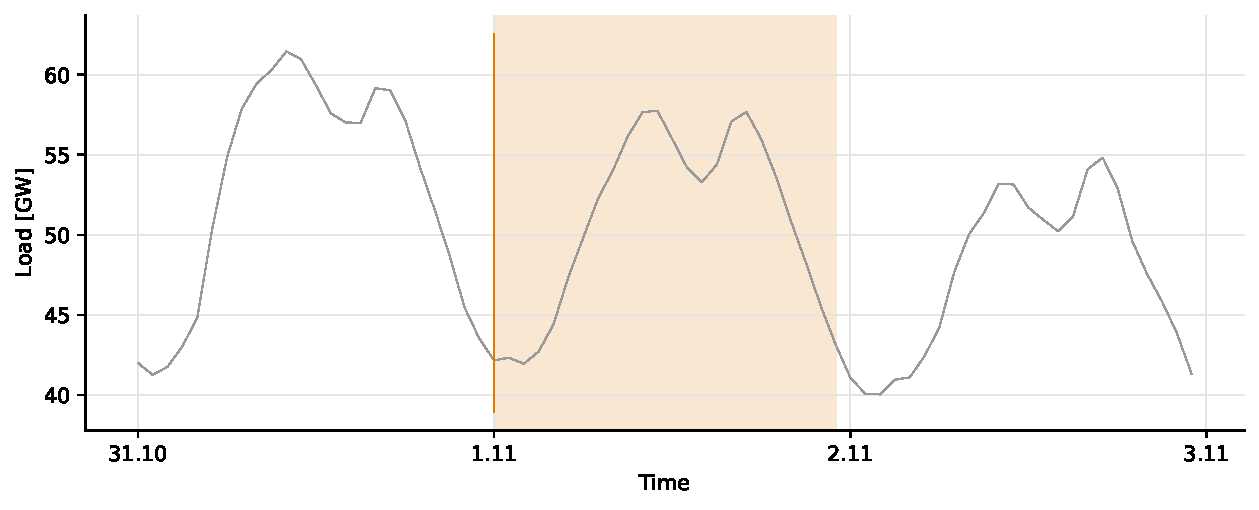
\includegraphics[keepaspectratio]{10_backtest_files/figure-pdf/fig-folds-output-1.pdf}}

}

\caption{\label{fig-folds}Visualisation of the rolling-origin folds. The
training range (blue) ends at the orange separator line at the start of
each fold. Each fold (orange-red) forecasts the following 24 hours. The
ENTSO-E load in the background (grey) provides context.}

\end{figure}%

\section{Distribution of errors across
folds}\label{distribution-of-errors-across-folds}

\begin{Shaded}
\begin{Highlighting}[]
\ImportTok{import}\NormalTok{ numpy }\ImportTok{as}\NormalTok{ np}

\CommentTok{\# MAE per fold}
\NormalTok{mae\_per\_fold }\OperatorTok{=}\NormalTok{ []}
\ControlFlowTok{for}\NormalTok{ i }\KeywordTok{in} \BuiltInTok{range}\NormalTok{(}\BuiltInTok{len}\NormalTok{(metrics\_df)):}
\NormalTok{    fold\_idx }\OperatorTok{=}\NormalTok{ predictions\_df.index[i }\OperatorTok{*} \DecValTok{24}\NormalTok{ : (i }\OperatorTok{+} \DecValTok{1}\NormalTok{) }\OperatorTok{*} \DecValTok{24}\NormalTok{]}
\NormalTok{    pred\_vals }\OperatorTok{=}\NormalTok{ predictions\_df.iloc[i }\OperatorTok{*} \DecValTok{24}\NormalTok{ : (i }\OperatorTok{+} \DecValTok{1}\NormalTok{) }\OperatorTok{*} \DecValTok{24}\NormalTok{, }\DecValTok{0}\NormalTok{].values}
\NormalTok{    actual }\OperatorTok{=}\NormalTok{ y\_bt.loc[fold\_idx].values}
\NormalTok{    mae\_per\_fold.append(np.}\BuiltInTok{abs}\NormalTok{(pred\_vals }\OperatorTok{{-}}\NormalTok{ actual).mean())}
\NormalTok{mae\_per\_fold }\OperatorTok{=}\NormalTok{ np.array(mae\_per\_fold) }\OperatorTok{/} \DecValTok{1000}   \CommentTok{\# in GW}

\NormalTok{fig, ax }\OperatorTok{=}\NormalTok{ plt.subplots(figsize}\OperatorTok{=}\NormalTok{(}\FloatTok{8.5}\NormalTok{, }\FloatTok{3.0}\NormalTok{))}
\NormalTok{ax.hist(mae\_per\_fold, bins}\OperatorTok{=}\DecValTok{12}\NormalTok{, color}\OperatorTok{=}\StringTok{"\#1F4E79"}\NormalTok{, alpha}\OperatorTok{=}\FloatTok{0.85}\NormalTok{, edgecolor}\OperatorTok{=}\StringTok{"white"}\NormalTok{)}
\NormalTok{ax.axvline(np.median(mae\_per\_fold), color}\OperatorTok{=}\StringTok{"\#E07B00"}\NormalTok{, linestyle}\OperatorTok{=}\StringTok{"{-}{-}"}\NormalTok{,}
\NormalTok{           linewidth}\OperatorTok{=}\FloatTok{1.2}\NormalTok{, label}\OperatorTok{=}\SpecialStringTok{f"Median = }\SpecialCharTok{\{}\NormalTok{np}\SpecialCharTok{.}\NormalTok{median(mae\_per\_fold)}\SpecialCharTok{:.2f\}}\SpecialStringTok{ GW"}\NormalTok{)}
\NormalTok{ax.axvline(mae\_per\_fold.}\BuiltInTok{max}\NormalTok{(), color}\OperatorTok{=}\StringTok{"\#B33A3A"}\NormalTok{, linewidth}\OperatorTok{=}\FloatTok{1.2}\NormalTok{,}
\NormalTok{           label}\OperatorTok{=}\SpecialStringTok{f"Maximum = }\SpecialCharTok{\{}\NormalTok{mae\_per\_fold}\SpecialCharTok{.}\BuiltInTok{max}\NormalTok{()}\SpecialCharTok{:.2f\}}\SpecialStringTok{ GW"}\NormalTok{)}
\NormalTok{ax.set\_xlabel(}\StringTok{"MAE per 24{-}h fold [GW]"}\NormalTok{)}
\NormalTok{ax.set\_ylabel(}\StringTok{"Number of folds"}\NormalTok{)}
\NormalTok{ax.legend(loc}\OperatorTok{=}\StringTok{"upper right"}\NormalTok{, frameon}\OperatorTok{=}\VariableTok{False}\NormalTok{)}
\NormalTok{ax.grid(}\VariableTok{True}\NormalTok{, color}\OperatorTok{=}\StringTok{"\#E5E5E5"}\NormalTok{, linewidth}\OperatorTok{=}\FloatTok{0.5}\NormalTok{)}
\ControlFlowTok{for}\NormalTok{ s }\KeywordTok{in}\NormalTok{ (}\StringTok{"top"}\NormalTok{, }\StringTok{"right"}\NormalTok{):}
\NormalTok{    ax.spines[s].set\_visible(}\VariableTok{False}\NormalTok{)}
\NormalTok{fig.tight\_layout()}
\NormalTok{plt.show()}
\end{Highlighting}
\end{Shaded}

\begin{figure}[H]

\centering{

\pandocbounded{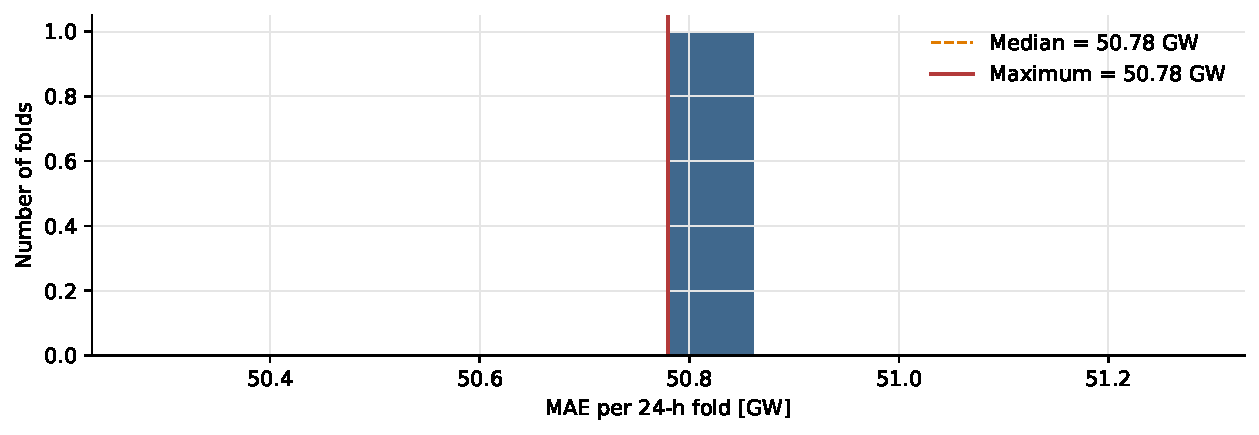
\includegraphics[keepaspectratio]{10_backtest_files/figure-pdf/fig-fold-distribution-output-1.pdf}}

}

\caption{\label{fig-fold-distribution}Distribution of MAE values across
all folds of the backtest, plus the median (dashed) and the maximum
value (red line). A narrow distribution means that the model quality is
consistent across the evaluation range.}

\end{figure}%

\begin{tcolorbox}[enhanced jigsaw, arc=.35mm, bottomrule=.15mm, bottomtitle=1mm, breakable, colback=white, colbacktitle=quarto-callout-tip-color!10!white, colframe=quarto-callout-tip-color-frame, coltitle=black, left=2mm, leftrule=.75mm, opacityback=0, opacitybacktitle=0.6, rightrule=.15mm, title=\textcolor{quarto-callout-tip-color}{\faLightbulb}\hspace{0.5em}{Exercises (with Claude)}, titlerule=0mm, toprule=.15mm, toptitle=1mm]

\begin{enumerate}
\def\labelenumi{\arabic{enumi}.}
\tightlist
\item
  \emph{Change \texttt{refit}.} Have Claude explain what changes about
  the evaluation when \texttt{refit=True} is set --- and how training
  cost and accuracy trade off. In which practical situation is weekly
  re-training worth it?
\item
  \emph{Adversarial fold.} Ask Claude to identify a fold in which the
  model performs particularly poorly and to discuss which data
  constellation might be responsible (holiday, weather event, load
  peak).
\item
  \emph{Robustness threshold.} Discuss with Claude how you would
  formulate an audit threshold above which a fold is marked as
  ``non-compliant'' --- and which actions should follow (model freeze,
  escalation to dispatcher, fallback).
\end{enumerate}

\end{tcolorbox}

\bookmarksetup{startatroot}

\chapter{Provenance and reproducibility}\label{sec-provenance}

\begin{tcolorbox}[enhanced jigsaw, arc=.35mm, bottomrule=.15mm, bottomtitle=1mm, breakable, colback=white, colbacktitle=quarto-callout-note-color!10!white, colframe=quarto-callout-note-color-frame, coltitle=black, left=2mm, leftrule=.75mm, opacityback=0, opacitybacktitle=0.6, rightrule=.15mm, title=\textcolor{quarto-callout-note-color}{\faInfo}\hspace{0.5em}{Learning objective}, titlerule=0mm, toprule=.15mm, toptitle=1mm]

You can derive, from a trained forecaster and its audit log, the minimum
amount of provenance information required by Art. 11 (technical
documentation) and Art. 12 (record-keeping) of the AI Act --- and you
can explain how all four code rules together guarantee the
reproducibility of a forecast across years.

\end{tcolorbox}

\section{What is this about?}\label{what-is-this-about}

Imagine that in two years' time a supervisory authority asks about a
load forecast our system produced on 28 November 2024 at 06:00 for the
following day. Can we, today, reproduce that forecast exactly as it was
generated back then? If yes, the system is \emph{auditable}. If not, the
authority is entitled to forbid further operation.

Reproducibility presupposes that we have documented all inputs,
hyperparameters and intermediate results completely enough for someone
running the same code to arrive at the exact same forecast. This chapter
is a retrospective: all four code rules and several AI Act articles come
together here.

\section{\texorpdfstring{Which fields does \texttt{spotforecast2-safe}
record
automatically?}{Which fields does spotforecast2-safe record automatically?}}\label{which-fields-does-spotforecast2-safe-record-automatically}

\protect\phantomsection\label{load-and-introspect}
\begin{Shaded}
\begin{Highlighting}[]
\ImportTok{import}\NormalTok{ json}
\ImportTok{import}\NormalTok{ pandas }\ImportTok{as}\NormalTok{ pd}
\ImportTok{import}\NormalTok{ pickle}
\ImportTok{from}\NormalTok{ pathlib }\ImportTok{import}\NormalTok{ Path}

\NormalTok{shared }\OperatorTok{=}\NormalTok{ Path(}\StringTok{"\_cache/shared"}\NormalTok{)}
\ControlFlowTok{with}\NormalTok{ Path(}\StringTok{"\_cache/forecaster.pkl"}\NormalTok{).}\BuiltInTok{open}\NormalTok{(}\StringTok{"rb"}\NormalTok{) }\ImportTok{as}\NormalTok{ fh:}
\NormalTok{    model }\OperatorTok{=}\NormalTok{ pickle.load(fh)}

\NormalTok{provenance }\OperatorTok{=}\NormalTok{ \{}
    \StringTok{"model\_name"}\NormalTok{:            model.name,}
    \StringTok{"estimator"}\NormalTok{:             }\BuiltInTok{type}\NormalTok{(model.forecaster.estimator).}\VariableTok{\_\_name\_\_}\NormalTok{,}
    \StringTok{"number\_of\_trees"}\NormalTok{:       }\BuiltInTok{int}\NormalTok{(model.forecaster.estimator.n\_estimators),}
    \StringTok{"learning\_rate"}\NormalTok{:         }\BuiltInTok{float}\NormalTok{(model.forecaster.estimator.learning\_rate),}
    \StringTok{"lags"}\NormalTok{:                  }\BuiltInTok{int}\NormalTok{(model.forecaster.lags.size),}
    \StringTok{"seed"}\NormalTok{:                  }\BuiltInTok{int}\NormalTok{(model.random\_state),}
    \StringTok{"training\_index\_from"}\NormalTok{:   }\BuiltInTok{str}\NormalTok{(model.forecaster.training\_range\_[}\DecValTok{0}\NormalTok{]),}
    \StringTok{"training\_index\_to"}\NormalTok{:     }\BuiltInTok{str}\NormalTok{(model.forecaster.training\_range\_[}\DecValTok{1}\NormalTok{]),}
    \StringTok{"calendar\_country"}\NormalTok{:      model.preprocessor.country\_code,}
    \StringTok{"number\_of\_periods"}\NormalTok{:     }\BuiltInTok{len}\NormalTok{(model.preprocessor.periods),}
    \StringTok{"exog\_column\_count"}\NormalTok{:     }\BuiltInTok{int}\NormalTok{(}\BuiltInTok{len}\NormalTok{(model.forecaster.exog\_names\_in\_ }\KeywordTok{or}\NormalTok{ [])),}
\NormalTok{\}}
\BuiltInTok{print}\NormalTok{(json.dumps(provenance, indent}\OperatorTok{=}\DecValTok{2}\NormalTok{, ensure\_ascii}\OperatorTok{=}\VariableTok{False}\NormalTok{))}
\end{Highlighting}
\end{Shaded}

\begin{verbatim}
{
  "model_name": "lgbm",
  "estimator": "LGBMRegressor",
  "number_of_trees": 400,
  "learning_rate": 0.05,
  "lags": 168,
  "seed": 2026,
  "training_index_from": "2024-01-01 00:00:00+00:00",
  "training_index_to": "2024-10-31 23:00:00+00:00",
  "calendar_country": "DE",
  "number_of_periods": 3,
  "exog_column_count": 45
}
\end{verbatim}

\section{Data provenance from the audit
log}\label{data-provenance-from-the-audit-log}

The log switched on in Chapter~\ref{sec-audit} contains every data
action: ENTSO-E download, weather fetch, gap handling, training,
prediction. We extract the file names and timestamps:

\protect\phantomsection\label{log-summary}
\begin{Shaded}
\begin{Highlighting}[]
\NormalTok{log\_dir }\OperatorTok{=}\NormalTok{ Path(}\StringTok{"\_cache/logs"}\NormalTok{)}
\NormalTok{log\_files }\OperatorTok{=} \BuiltInTok{sorted}\NormalTok{(log\_dir.glob(}\StringTok{"*.log"}\NormalTok{)) }\ControlFlowTok{if}\NormalTok{ log\_dir.exists() }\ControlFlowTok{else}\NormalTok{ []}
\ControlFlowTok{if}\NormalTok{ log\_files:}
\NormalTok{    latest }\OperatorTok{=}\NormalTok{ log\_files[}\OperatorTok{{-}}\DecValTok{1}\NormalTok{]}
\NormalTok{    lines }\OperatorTok{=}\NormalTok{ latest.read\_text().splitlines()}
    \BuiltInTok{print}\NormalTok{(}\SpecialStringTok{f"Log file: }\SpecialCharTok{\{}\NormalTok{latest}\SpecialCharTok{.}\NormalTok{name}\SpecialCharTok{\}}\SpecialStringTok{, }\SpecialCharTok{\{}\BuiltInTok{len}\NormalTok{(lines)}\SpecialCharTok{\}}\SpecialStringTok{ lines"}\NormalTok{)}
    \BuiltInTok{print}\NormalTok{()}
    \BuiltInTok{print}\NormalTok{(}\StringTok{"First five entries:"}\NormalTok{)}
    \ControlFlowTok{for}\NormalTok{ line }\KeywordTok{in}\NormalTok{ lines[:}\DecValTok{5}\NormalTok{]:}
        \BuiltInTok{print}\NormalTok{(}\StringTok{"  "} \OperatorTok{+}\NormalTok{ line)}
\ControlFlowTok{else}\NormalTok{:}
    \BuiltInTok{print}\NormalTok{(}\StringTok{"No log files found."}\NormalTok{)}
\end{Highlighting}
\end{Shaded}

\begin{verbatim}
Log file: task_safe_n_to_1_20260531_215057.log, 2 lines

First five entries:
  {"schema_version":"1.0.0","timestamp_utc":"2026-05-31T19:50:57.585840Z","logger":"task_safe_n_to_1","level":"INFO","event":"audit_log_init","message":"Persistent logging initialized at: _cache/logs/task_safe_n_to_1_20260531_215057.log"}
  {"schema_version":"1.0.0","timestamp_utc":"2026-05-31T19:50:57.586367Z","logger":"task_safe_n_to_1","level":"INFO","event":"log","message":"Course run starts: load-forecasting pipeline (chapter 01)."}
\end{verbatim}

\section{Visualisation: the provenance
diagram}\label{visualisation-the-provenance-diagram}

The following Mermaid diagram summarises the data and control flows of
the entire pipeline. In this form it can be reused directly in a
\texttt{MODEL\_CARD.md}.

\begin{Shaded}
\begin{Highlighting}[]
\NormalTok{flowchart TD}
\NormalTok{    A["ENTSO{-}E API\textless{}br/\textgreater{}(Country=DE, 2024)"] {-}{-}\textgreater{}|download\_new\_data| B["raw CSVs"]}
\NormalTok{    B {-}{-}\textgreater{}|merge\_build\_manual| C["interim/energy\_load.csv"]}
\NormalTok{    O["Open{-}Meteo Archive API\textless{}br/\textgreater{}(50.11N, 8.68E)"] {-}{-}\textgreater{}|WeatherService.get\_dataframe| W["weather\_de\_2024.parquet"]}
\NormalTok{    C {-}{-}\textgreater{} D["LinearlyInterpolateTS\textless{}br/\textgreater{}(on\_missing=raise)"]}
\NormalTok{    D {-}{-}\textgreater{} E["y\_train + y\_eval\textless{}br/\textgreater{}chronological split"]}
\NormalTok{    W {-}{-}\textgreater{} F["ExogBuilder\textless{}br/\textgreater{}(periods + holidays)"]}
\NormalTok{    F {-}{-}\textgreater{} G["exog.parquet"]}
\NormalTok{    E {-}{-}\textgreater{} H["ForecasterRecursiveLGBM\textless{}br/\textgreater{}(seed=2026, lags=168)"]}
\NormalTok{    G {-}{-}\textgreater{} H}
\NormalTok{    H {-}{-}\textgreater{}|fit| M["forecaster.pkl"]}
\NormalTok{    M {-}{-}\textgreater{}|predict| P["y\_pred\_24h.parquet"]}
\NormalTok{    M {-}{-}\textgreater{}|backtesting\_forecaster| BT["metrics\_df + predictions\_df"]}
\NormalTok{    H {-}{-}\textgreater{} L["Audit log\textless{}br/\textgreater{}(\_cache/logs/*.log)"]}
\end{Highlighting}
\end{Shaded}

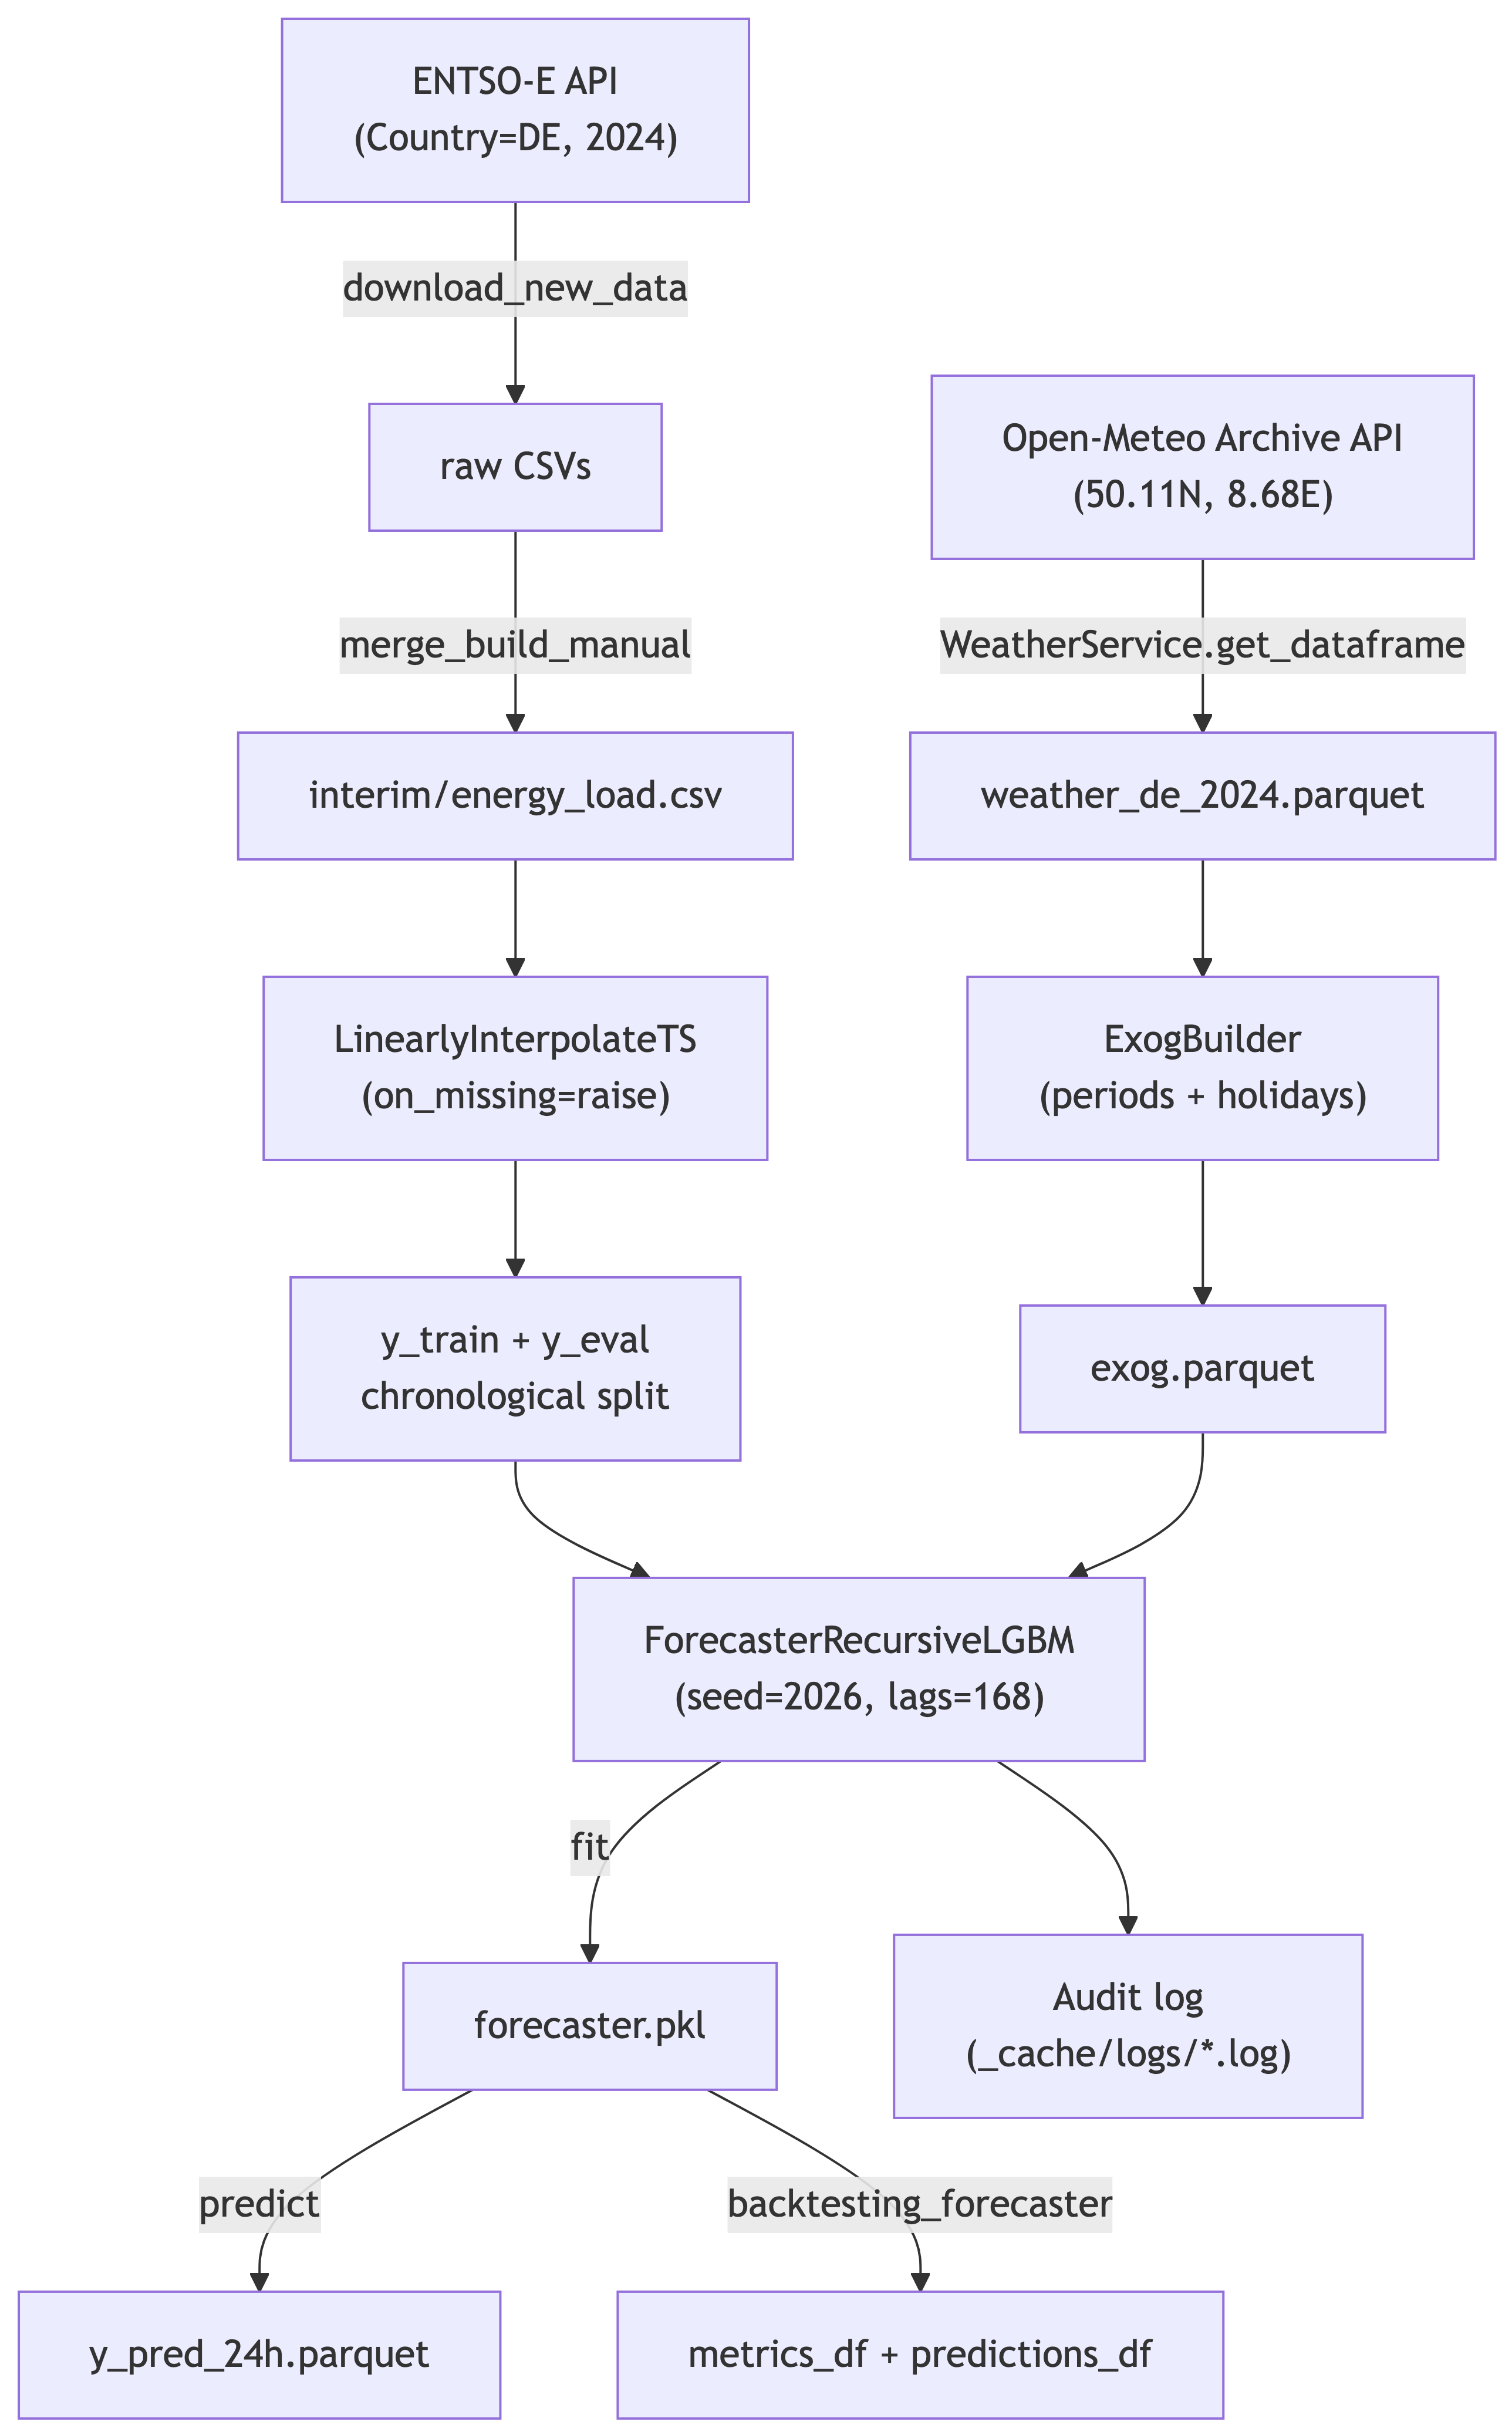
\includegraphics[width=6.72in,height=10.81in]{11_provenance_files/figure-latex/mermaid-figure-1.png}

\section{How all four code rules come together
here}\label{how-all-four-code-rules-come-together-here}

{\def\LTcaptype{none} % do not increment counter
\begin{longtable}[]{@{}
  >{\centering\arraybackslash}p{(\linewidth - 2\tabcolsep) * \real{0.1250}}
  >{\raggedright\arraybackslash}p{(\linewidth - 2\tabcolsep) * \real{0.8750}}@{}}
\toprule\noalign{}
\begin{minipage}[b]{\linewidth}\centering
Code rule
\end{minipage} & \begin{minipage}[b]{\linewidth}\raggedright
Effect in this pipeline
\end{minipage} \\
\midrule\noalign{}
\endhead
\bottomrule\noalign{}
\endlastfoot
CR-1 & Every function (\texttt{download\_new\_data},
\texttt{LinearlyInterpolateTS}, \texttt{ExogBuilder},
\texttt{WeatherService}, \texttt{ForecasterRecursiveLGBM},
\texttt{backtesting\_forecaster}) is represented in the logging and
protected by tests. \\
CR-2 & Fixed date constants, fixed seed, \texttt{deterministic=True} in
LightGBM, fixed \texttt{random\_state} --- bit-exact reproducibility
even after years. \\
CR-3 & NaN behaviour in \texttt{LinearlyInterpolateTS}
(\texttt{on\_missing=\textquotesingle{}raise\textquotesingle{}}) and in
\texttt{WeatherService} (\texttt{fill\_missing=False}) --- gaps are
reported, not silently filled. \\
CR-4 & Deny-list forbids \texttt{plotly}, \texttt{matplotlib},
\texttt{optuna}, \texttt{torch}, \texttt{tensorflow} as dependencies;
LightGBM and scikit-learn are allowed because they are small and well
maintained. \\
\end{longtable}
}

\section{AI Act link, compact}\label{ai-act-link-compact}

{\def\LTcaptype{none} % do not increment counter
\begin{longtable}[]{@{}
  >{\raggedright\arraybackslash}p{(\linewidth - 4\tabcolsep) * \real{0.2604}}
  >{\raggedright\arraybackslash}p{(\linewidth - 4\tabcolsep) * \real{0.1042}}
  >{\raggedright\arraybackslash}p{(\linewidth - 4\tabcolsep) * \real{0.6354}}@{}}
\toprule\noalign{}
\begin{minipage}[b]{\linewidth}\raggedright
Obligation
\end{minipage} & \begin{minipage}[b]{\linewidth}\raggedright
Article
\end{minipage} & \begin{minipage}[b]{\linewidth}\raggedright
Fulfilled in the pipeline by
\end{minipage} \\
\midrule\noalign{}
\endhead
\bottomrule\noalign{}
\endlastfoot
Risk management & Art. 9 & Backtest in Chapter~\ref{sec-backtest},
deterministic training, audit log \\
Data governance & Art. 10 & Provenance note from chapter 02, NaN
discipline from Chapter~\ref{sec-missing}, weather fail-safe \\
Technical documentation & Art. 11 & Provenance diagram, JSON entry
above, MODEL\_CARD.md in the package \\
Record-keeping & Art. 12 & Audit log, persisted intermediate artefacts
(\texttt{*.parquet}, \texttt{*.pkl}) \\
Transparency & Art. 13 & Feature-importance plot in
Chapter~\ref{sec-train}, recursion equation in
Chapter~\ref{sec-forecast} \\
Accuracy/robustness & Art. 15 & Four metrics in
Chapter~\ref{sec-accuracy} plus backtest distribution \\
\end{longtable}
}

\section{Persisting the provenance
note}\label{persisting-the-provenance-note}

\protect\phantomsection\label{persist-provenance}
\begin{Shaded}
\begin{Highlighting}[]
\ImportTok{import}\NormalTok{ json}
\NormalTok{out }\OperatorTok{=}\NormalTok{ Path(}\StringTok{"\_cache/provenance.json"}\NormalTok{)}
\NormalTok{out.write\_text(json.dumps(provenance, indent}\OperatorTok{=}\DecValTok{2}\NormalTok{, ensure\_ascii}\OperatorTok{=}\VariableTok{False}\NormalTok{))}
\BuiltInTok{print}\NormalTok{(}\SpecialStringTok{f"Provenance note: }\SpecialCharTok{\{}\NormalTok{out}\SpecialCharTok{\}}\SpecialStringTok{"}\NormalTok{)}
\end{Highlighting}
\end{Shaded}

\begin{verbatim}
Provenance note: _cache/provenance.json
\end{verbatim}

\begin{tcolorbox}[enhanced jigsaw, arc=.35mm, bottomrule=.15mm, bottomtitle=1mm, breakable, colback=white, colbacktitle=quarto-callout-tip-color!10!white, colframe=quarto-callout-tip-color-frame, coltitle=black, left=2mm, leftrule=.75mm, opacityback=0, opacitybacktitle=0.6, rightrule=.15mm, title=\textcolor{quarto-callout-tip-color}{\faLightbulb}\hspace{0.5em}{Exercises (with Claude)}, titlerule=0mm, toprule=.15mm, toptitle=1mm]

\begin{enumerate}
\def\labelenumi{\arabic{enumi}.}
\tightlist
\item
  \emph{Reproduction in two years.} Ask Claude to sketch a concise
  recovery plan: an audit team wants to reproduce in 2027 the forecast
  from 28 November 2024 for 29 November 2024. Which five artefacts of
  this pipeline are needed at minimum? Which code rules make this
  endeavour possible at all?
\item
  \emph{Gap analysis.} Discuss with Claude which additional provenance
  fields \emph{beyond} the list printed here should appear in a real
  \texttt{MODEL\_CARD.md} (e.g.~hash of the training data, versions of
  every dependency, hardware description). Which standard expressly
  requires these fields (AI Act, IEC 62443, ISO 25059)?
\item
  \emph{Audit script.} Have Claude write a small Python script that
  reads the persisted \texttt{provenance.json} and automatically checks
  whether all mandatory fields are populated. Which code rule is the
  prerequisite for such an automated check to be meaningful at all?
\end{enumerate}

\end{tcolorbox}

\section{Closing remark}\label{closing-remark}

In ten chapters you have built a complete safety-critical
load-forecasting pipeline: from live data acquisition through cyclic
features, weather, deterministic training, prediction, accuracy
measurement and backtest, all the way to a reproducible provenance note.
If you were now asked in an audit how you comply with the AI Act, you
can answer with \emph{code} instead of reassurances --- and that is
precisely the spirit in which \texttt{spotforecast2-safe} was developed.

\bookmarksetup{startatroot}

\chapter{Challenge: live load forecasting}\label{sec-challenge}

\begin{tcolorbox}[enhanced jigsaw, arc=.35mm, bottomrule=.15mm, bottomtitle=1mm, breakable, colback=white, colbacktitle=quarto-callout-note-color!10!white, colframe=quarto-callout-note-color-frame, coltitle=black, left=2mm, leftrule=.75mm, opacityback=0, opacitybacktitle=0.6, rightrule=.15mm, title=\textcolor{quarto-callout-note-color}{\faInfo}\hspace{0.5em}{Learning objective}, titlerule=0mm, toprule=.15mm, toptitle=1mm]

You take the pipeline learned in chapters 01-11 into a \textbf{live}
24-hour load forecast, submit a prediction for the next day every day,
and defend your submission in an auditing sense (CR-1 to CR-4, Art. 10,
12, 13, 15 of the AI Act). Evaluation is automatic against the ENTSO-E
ground truth; the leaderboard is updated weekly.

\end{tcolorbox}

\section{Why a live challenge?}\label{why-a-live-challenge}

Chapters 02-11 deliberately use a \textbf{frozen} time slice
(\texttt{DATA\_START\ =\ 2024-01-01}, \texttt{DATA\_END\ =\ 2024-12-31})
so that every student obtains byte-identical results (CR-2). That
advantage disappears the moment the model is to run \emph{in
production}: new measurements arrive every hour, forecasters are
retrained on a rolling window, gaps appear unpredictably, and the AI Act
still demands a verifiable audit trail (Art. 12) and robustness against
distribution drift (Art. 15).

The challenge simulates this live setting. You submit a forecast every
day; an automatic evaluation workflow compares it the next day with the
value finally published by ENTSO-E. The setup is modelled on the
well-known scientific competitions:

\begin{itemize}
\tightlist
\item
  \textbf{GEFCom 2012/2014/2017} (Hong et al. 2014, 2016, 2019) --- the
  Global Energy Forecasting Competition, the academic standard for
  load-forecasting competitions (IEEE Working Group /
  \emph{International Journal of Forecasting}).
\item
  \textbf{M4 / M5 / M6} (Makridakis et al. 2020, 2022) --- the
  Makridakis competitions that have established conventions for rolling
  backtesting and point/quantile evaluation.
\item
  \textbf{EEM Forecasting Competitions} (IEEE European Energy Market) as
  a recurring European annual format.
\item
  \textbf{BDEW standard load profiles} as a German industry benchmark.
\end{itemize}

Methodologically this challenge closely follows GEFCom 2017
(hierarchical load forecasting) and M4 (rolling one-step-ahead setup).

\section{AI Act link}\label{ai-act-link-7}

{\def\LTcaptype{none} % do not increment counter
\begin{longtable}[]{@{}
  >{\raggedright\arraybackslash}p{(\linewidth - 4\tabcolsep) * \real{0.6951}}
  >{\raggedright\arraybackslash}p{(\linewidth - 4\tabcolsep) * \real{0.1463}}
  >{\raggedright\arraybackslash}p{(\linewidth - 4\tabcolsep) * \real{0.1585}}@{}}
\toprule\noalign{}
\begin{minipage}[b]{\linewidth}\raggedright
Challenge rule
\end{minipage} & \begin{minipage}[b]{\linewidth}\raggedright
Code rule
\end{minipage} & \begin{minipage}[b]{\linewidth}\raggedright
AI Act
\end{minipage} \\
\midrule\noalign{}
\endhead
\bottomrule\noalign{}
\endlastfoot
Submission deadline \emph{before} availability of target hours & CR-3 &
Art. 10, 15 \\
Completeness of submission (24 rows, no NaN) & CR-3 & Art. 10 \\
Git commit timestamps auditable in CI & CR-1 & Art. 12 \\
Score run deterministically reproducible & CR-2 & Art. 12, 15 \\
Pinned pipeline dependencies (uv.lock) & CR-4 & Art. 15 \\
Ground-truth source documented (ENTSO-E final) & CR-1 & Art. 10, 13 \\
\end{longtable}
}

\section{Rules at a glance}\label{rules-at-a-glance}

{\def\LTcaptype{none} % do not increment counter
\begin{longtable}[]{@{}
  >{\raggedright\arraybackslash}p{(\linewidth - 2\tabcolsep) * \real{0.2804}}
  >{\raggedright\arraybackslash}p{(\linewidth - 2\tabcolsep) * \real{0.7196}}@{}}
\toprule\noalign{}
\begin{minipage}[b]{\linewidth}\raggedright
Aspect
\end{minipage} & \begin{minipage}[b]{\linewidth}\raggedright
Definition
\end{minipage} \\
\midrule\noalign{}
\endhead
\bottomrule\noalign{}
\endlastfoot
Target variable & DE hourly load \texttt{Actual\ Load} {[}MW{]} from the
ENTSO-E Transparency Platform \\
Horizon & 24 h (00:00-23:00 CET of target day \emph{D}) \\
Submission cadence & daily, one entry per team \\
Deadline (target day \emph{D}) & \emph{D-1} 23:59 CET --- later-arriving
PRs are rejected \\
Ground-truth availability & \emph{D+1} around 06:00 UTC (ENTSO-E
\emph{final values}) \\
Score run & daily \emph{D+1} 07:00 UTC via GitHub Actions cron \\
Primary metric & \textbf{MAE} {[}MW{]} over the 24 hours \\
Ranking (public) & \textbf{Rolling 7-day mean MAE} --- moving weekly
average \\
Tie-break 1 & cumulative MAE since kickoff (smaller wins) \\
Tie-break 2 & number of valid submissions (more wins) \\
Anti-leakage & Deadline lies \emph{before} the first target hour; commit
timestamps verifiable in CI \\
Leaderboard refresh & after every score run (daily); weekly snapshot
Sunday 23:55 UTC \\
\end{longtable}
}

For orientation: the \emph{state-of-the-art} accuracy for the German
day-ahead load forecast is around MAPE \textasciitilde3 \%. A simple
\textbf{weekly persistence} (load exactly 168 h earlier) typically
yields MAPE 5-7 \% and is a useful sanity check (see
Chapter~\ref{sec-accuracy}).

\section{Participation}\label{participation}

\begin{itemize}
\tightlist
\item
  \textbf{Team size}: 2-4 people. Solo participation is not foreseen.
\item
  \textbf{Registration}: until 12 May 2026 (Tuesday) by email to Prof.
  Bartz-Beielstein, with (i) team name, (ii) team ID (short, lowercase,
  no space, e.g.~\texttt{team\_lambda}), (iii) GitHub handles of all
  members.
\item
  One person from the team is registered in \texttt{teams.yml} as the
  submission owner; however, every team member may submit via PR.
\end{itemize}

\section{GitHub onboarding}\label{sec-github-onboarding}

Technically the challenge runs on GitHub. If you have never worked with
it, get yourself up to speed in three steps here: create an account,
find your handle, set up authentication. If you already use GitHub
actively, you can skip this section and jump straight to
Section~\ref{sec-submission-workflow}.

\begin{tcolorbox}[enhanced jigsaw, arc=.35mm, bottomrule=.15mm, bottomtitle=1mm, breakable, colback=white, colbacktitle=quarto-callout-note-color!10!white, colframe=quarto-callout-note-color-frame, coltitle=black, left=2mm, leftrule=.75mm, opacityback=0, opacitybacktitle=0.6, rightrule=.15mm, title=\textcolor{quarto-callout-note-color}{\faInfo}\hspace{0.5em}{Learning objective}, titlerule=0mm, toprule=.15mm, toptitle=1mm]

You have a GitHub account, know your handle, have forked the leaderboard
repo and cloned it locally. \texttt{git\ push} and \texttt{git\ pull}
work without a password prompt.

\end{tcolorbox}

\subsection{What is GitHub, what is your
handle?}\label{what-is-github-what-is-your-handle}

\textbf{GitHub} is a public hosting service for Git repositories
(\url{https://github.com/}). Every account has a unique \emph{username},
also called \emph{handle} or \emph{login}. The handle is always
identical to the final URL component of your profile:

\begin{verbatim}
https://github.com/<handle>
\end{verbatim}

Format: 1-39 characters, letters/digits/hyphen, no umlauts. GitHub
ignores case when comparing --- internally everything is normalised to
lowercase.

\textbf{Why the handle matters here.} Submissions go through pull
requests. The CI workflow \texttt{validate-pr.yml} in the leaderboard
repository reads the author's \emph{login} from the GitHub event when a
PR arrives and compares it with the \texttt{github\_handles} list of the
relevant team in \texttt{teams.yml}. Anyone not on that list gets:

\begin{verbatim}
ERROR: PR author 'X' not in github_handles for team 'T': [...]
\end{verbatim}

This implements CR-1 (identity \& auditability): only you and your team
members can submit \emph{on behalf of your team}.

\subsection{Create an account}\label{create-an-account}

\begin{enumerate}
\def\labelenumi{\arabic{enumi}.}
\tightlist
\item
  Open \url{https://github.com/signup}.
\item
  Pick an email, password and \emph{username}. \textbf{Important:} the
  username is your future handle and should look professionally solid
  (\texttt{tina.musterhuhn} looks more serious than
  \texttt{xxtina4lifexx}).
\item
  Click through the email confirmation.
\item
  Activate two-factor authentication (Settings -\textgreater{} Password
  and authentication -\textgreater{} Two-factor authentication). A TOTP
  app like Aegis or 1Password suffices.
\end{enumerate}

\subsection{Find your handle (for the registration
email)}\label{find-your-handle-for-the-registration-email}

Two reliable ways:

\begin{itemize}
\tightlist
\item
  \textbf{Click the profile picture top right} --- the first menu item
  (``Your profile'') shows your handle.
\item
  \textbf{In any profile URL.} Visiting \url{https://github.com/} while
  logged in redirects to
  \texttt{https://github.com/\textless{}handle\textgreater{}}.
\end{itemize}

\begin{tcolorbox}[enhanced jigsaw, arc=.35mm, bottomrule=.15mm, bottomtitle=1mm, breakable, colback=white, colbacktitle=quarto-callout-important-color!10!white, colframe=quarto-callout-important-color-frame, coltitle=black, left=2mm, leftrule=.75mm, opacityback=0, opacitybacktitle=0.6, rightrule=.15mm, title=\textcolor{quarto-callout-important-color}{\faExclamation}\hspace{0.5em}{Send handles to the lecturer}, titlerule=0mm, toprule=.15mm, toptitle=1mm]

Send \emph{all} handles of your team in the registration email,
otherwise individual members will later be unable to submit PRs. Format
like the example below:

\begin{quote}
\emph{Registration team ``Lambda Forecasters''}\\
\emph{Team-ID: \texttt{team\_lambda}}\\
\emph{Members and handles:}

\begin{itemize}
\tightlist
\item
  \emph{Alice Mueller --- GitHub: \texttt{alice42}}
\item
  \emph{Bob Schmidt --- GitHub: \texttt{bob99}}
\item
  \emph{Carol Schulze --- GitHub: \texttt{carol7}}
\end{itemize}
\end{quote}

Corrections are possible at any time but cost one cycle: you report the
fix by email, the lecturer commits the changed \texttt{teams.yml}, and
you push a new (or empty) commit on your PR so that CI revalidates.

\end{tcolorbox}

\subsection{Set up authentication
locally}\label{set-up-authentication-locally}

Otherwise \texttt{git\ push} asks for a password every time. Choose
\emph{one} of the two variants.

\textbf{Variant A --- SSH key (recommended for daily use).}

\begin{Shaded}
\begin{Highlighting}[]
\FunctionTok{ssh{-}keygen} \AttributeTok{{-}t}\NormalTok{ ed25519 }\AttributeTok{{-}C} \StringTok{"your.address@th{-}koeln.de"}
\CommentTok{\# Copy the public key (\textasciitilde{}/.ssh/id\_ed25519.pub) to the clipboard:}
\FunctionTok{cat}\NormalTok{ \textasciitilde{}/.ssh/id\_ed25519.pub}
\end{Highlighting}
\end{Shaded}

Then on \url{https://github.com/settings/keys} -\textgreater{} \emph{New
SSH key} -\textgreater{} paste contents -\textgreater{} save. Test:
\texttt{ssh\ -T\ git@github.com}.

\textbf{Variant B --- HTTPS with Personal Access Token.}

GitHub -\textgreater{} Settings -\textgreater{} Developer settings
-\textgreater{} Personal access tokens -\textgreater{}
\emph{Fine-grained tokens} -\textgreater{} \emph{Generate new token}.
Scope: read/write on the fork of the leaderboard repo. Enter the token
as a password on the first \texttt{git\ push}; Git stores it in the
credential helper.

\subsection{\texorpdfstring{Install the \texttt{gh} CLI (optional but
practical)}{Install the gh CLI (optional but practical)}}\label{install-the-gh-cli-optional-but-practical}

\texttt{gh} is GitHub's official command-line tool. It lets you fork,
open and merge PRs without touching the browser.

\begin{Shaded}
\begin{Highlighting}[]
\CommentTok{\# macOS:}
\ExtensionTok{brew}\NormalTok{ install gh}
\CommentTok{\# Windows:}
\ExtensionTok{winget}\NormalTok{ install }\AttributeTok{{-}{-}id}\NormalTok{ GitHub.cli}
\CommentTok{\# Linux (Debian/Ubuntu):}
\FunctionTok{sudo}\NormalTok{ apt install gh}
\end{Highlighting}
\end{Shaded}

One-off login: \texttt{gh\ auth\ login\ -\/-web}. Then
\texttt{gh\ auth\ status} is enough to check that everything is in
place.

\subsection{Fork and local clone}\label{fork-and-local-clone}

Before you can submit, you need a \textbf{fork} of the leaderboard repo
--- your own copy at
\texttt{https://github.com/\textless{}your-handle\textgreater{}/challenge-leaderboard}.
GitHub rejects direct pushes into the original repo (branch protection),
and that is intentional: everything goes through pull requests.

\textbf{Web UI:}

\begin{enumerate}
\def\labelenumi{\arabic{enumi}.}
\item
  Open \url{https://github.com/bartzbeielstein/challenge-leaderboard}.
\item
  Click \emph{Fork} top right -\textgreater{} Owner = your own account
  -\textgreater{} \emph{Create fork}.
\item
  On the fork page click \emph{Code} -\textgreater{} copy the SSH
  (\texttt{git@github.com:...}) or HTTPS
  (\texttt{https://github.com/...}) URL.
\item
  Locally:

\begin{Shaded}
\begin{Highlighting}[]
\FunctionTok{git}\NormalTok{ clone git@github.com:}\OperatorTok{\textless{}}\NormalTok{your{-}handle}\OperatorTok{\textgreater{}}\NormalTok{/challenge{-}leaderboard.git}
\BuiltInTok{cd}\NormalTok{ challenge{-}leaderboard}
\ExtensionTok{uv}\NormalTok{ sync}
\end{Highlighting}
\end{Shaded}
\end{enumerate}

\textbf{CLI:}

\begin{Shaded}
\begin{Highlighting}[]
\ExtensionTok{gh}\NormalTok{ repo fork bartzbeielstein/challenge{-}leaderboard }\AttributeTok{{-}{-}clone}
\BuiltInTok{cd}\NormalTok{ challenge{-}leaderboard}
\ExtensionTok{uv}\NormalTok{ sync}
\end{Highlighting}
\end{Shaded}

\texttt{uv\ sync} installs the Python dependencies pinned in the repo
--- identical to the stack the CI uses for validation (CR-2).

\section{Submission format}\label{submission-format}

A submission is a single CSV file with the following schema:

{\def\LTcaptype{none} % do not increment counter
\begin{longtable}[]{@{}
  >{\raggedright\arraybackslash}p{(\linewidth - 4\tabcolsep) * \real{0.1593}}
  >{\raggedright\arraybackslash}p{(\linewidth - 4\tabcolsep) * \real{0.1239}}
  >{\raggedright\arraybackslash}p{(\linewidth - 4\tabcolsep) * \real{0.7168}}@{}}
\toprule\noalign{}
\begin{minipage}[b]{\linewidth}\raggedright
Column
\end{minipage} & \begin{minipage}[b]{\linewidth}\raggedright
Type
\end{minipage} & \begin{minipage}[b]{\linewidth}\raggedright
Meaning
\end{minipage} \\
\midrule\noalign{}
\endhead
\bottomrule\noalign{}
\endlastfoot
\texttt{timestamp\_utc} & \texttt{str} (ISO) & hour start in UTC,
exactly 24 consecutive hours of the target day \emph{D} \\
\texttt{forecast\_mw} & \texttt{float} & predicted load value in
megawatts, strictly positive \\
\end{longtable}
}

Path convention in the leaderboard repository:

\begin{verbatim}
submissions/<team_id>/<YYYY-MM-DD>.csv
\end{verbatim}

Here \texttt{\textless{}YYYY-MM-DD\textgreater{}} is the target day
\emph{D} (the date \emph{for which} the forecast applies --- not the
submission day). Example: on 14 May 2026 at 17:30 team
\texttt{team\_lambda} submits the forecast for 15 May:

\begin{verbatim}
submissions/team_lambda/2026-05-15.csv
\end{verbatim}

A mini example of the CSV file (excerpt):

\protect\phantomsection\label{sample-csv}
\begin{Shaded}
\begin{Highlighting}[]
\ImportTok{import}\NormalTok{ pandas }\ImportTok{as}\NormalTok{ pd}

\NormalTok{sample }\OperatorTok{=}\NormalTok{ pd.DataFrame(\{}
    \StringTok{"timestamp\_utc"}\NormalTok{: [}
        \StringTok{"2026{-}05{-}15T00:00:00Z"}\NormalTok{,}
        \StringTok{"2026{-}05{-}15T01:00:00Z"}\NormalTok{,}
        \StringTok{"2026{-}05{-}15T02:00:00Z"}\NormalTok{,}
        \StringTok{"..."}\NormalTok{,}
        \StringTok{"2026{-}05{-}15T23:00:00Z"}\NormalTok{,}
\NormalTok{    ],}
    \StringTok{"forecast\_mw"}\NormalTok{: [}\FloatTok{48\_500.0}\NormalTok{, }\FloatTok{47\_200.0}\NormalTok{, }\FloatTok{46\_400.0}\NormalTok{, }\StringTok{"..."}\NormalTok{, }\FloatTok{52\_100.0}\NormalTok{],}
\NormalTok{\})}
\BuiltInTok{print}\NormalTok{(sample.to\_string(index}\OperatorTok{=}\VariableTok{False}\NormalTok{))}
\end{Highlighting}
\end{Shaded}

\begin{verbatim}
       timestamp_utc forecast_mw
2026-05-15T00:00:00Z     48500.0
2026-05-15T01:00:00Z     47200.0
2026-05-15T02:00:00Z     46400.0
                 ...         ...
2026-05-15T23:00:00Z     52100.0
\end{verbatim}

For a deviating schema (too many/few rows, missing column, wrong date,
\texttt{NaN} or negative values) the CI validation workflow rejects the
PR with a precise error line (CR-3).

\section{Submission workflow}\label{sec-submission-workflow}

Prep done (Section~\ref{sec-github-onboarding})? Then now follows the
daily routine. It consists of a \textbf{one-time setup} and a
\textbf{recurring submission cycle}.

\subsection{One-time setup --- preconditions
checklist}\label{one-time-setup-preconditions-checklist}

\begin{enumerate}
\def\labelenumi{\arabic{enumi}.}
\tightlist
\item
  Valid GitHub account and handle submitted to the lecturer
  (Section~\ref{sec-github-onboarding}).
\item
  Fork of the leaderboard repo created and cloned locally
  (\texttt{challenge-leaderboard/} on your disk).
\item
  \texttt{uv\ sync} run in the repo root --- the Python stack is in
  place.
\item
  \texttt{ENTSOE\_API\_KEY} is exported in the shell
  (\texttt{export\ ENTSOE\_API\_KEY=...}). Without this key the
  generator script cannot fetch real data.
\item
  The generator script \texttt{make\_submission.py} from the course repo
  is available (see Section~\ref{sec-baseline-skript}) --- or your own.
\end{enumerate}

\subsection{Submission cycle per target
day}\label{submission-cycle-per-target-day}

In the following, \texttt{\textless{}team\_id\textgreater{}} denotes
your team's ID (e.g. \texttt{team\_lambda}) and
\texttt{\textless{}D\textgreater{}} the target day in
\texttt{YYYY-MM-DD} format (e.g. \texttt{2026-05-13}).

\subsubsection{1. Produce the CSV}\label{produce-the-csv}

In the root directory of your local leaderboard fork:

\begin{Shaded}
\begin{Highlighting}[]
\BuiltInTok{cd}\NormalTok{ .../challenge{-}leaderboard}
\ExtensionTok{python}\NormalTok{ .../lecture/scripts/make\_submission.py }\DataTypeTok{\textbackslash{}}
    \AttributeTok{{-}{-}team} \OperatorTok{\textless{}}\NormalTok{team\_id}\OperatorTok{\textgreater{}}\NormalTok{ {-}{-}target{-}date }\OperatorTok{\textless{}}\NormalTok{D}\OperatorTok{\textgreater{}}
\end{Highlighting}
\end{Shaded}

The script writes the file to
\texttt{submissions/\textless{}team\_id\textgreater{}/\textless{}D\textgreater{}.csv}.
Inspect briefly: 24 rows, plausible values (DE load typically 40 000 -
70 000 MW).

\subsubsection{2. Create a feature
branch}\label{create-a-feature-branch}

One separate branch per submission.

\textbf{CLI:}

\begin{Shaded}
\begin{Highlighting}[]
\FunctionTok{git}\NormalTok{ switch }\AttributeTok{{-}c}\NormalTok{ submission/}\OperatorTok{\textless{}}\NormalTok{team\_id}\OperatorTok{\textgreater{}}\NormalTok{/}\OperatorTok{\textless{}}\NormalTok{D}\OperatorTok{\textgreater{}}
\end{Highlighting}
\end{Shaded}

\textbf{Web UI:} on
\texttt{https://github.com/\textless{}your-handle\textgreater{}/challenge-leaderboard}
open the branch dropdown top left, type the new branch name and confirm
with \emph{Create branch \ldots{}}. Then locally
\texttt{git\ fetch\ \&\&\ git\ switch\ submission/\textless{}team\_id\textgreater{}/\textless{}D\textgreater{}}.

\subsubsection{3. Add the CSV and commit}\label{add-the-csv-and-commit}

\begin{tcolorbox}[enhanced jigsaw, arc=.35mm, bottomrule=.15mm, bottomtitle=1mm, breakable, colback=white, colbacktitle=quarto-callout-warning-color!10!white, colframe=quarto-callout-warning-color-frame, coltitle=black, left=2mm, leftrule=.75mm, opacityback=0, opacitybacktitle=0.6, rightrule=.15mm, title=\textcolor{quarto-callout-warning-color}{\faExclamationTriangle}\hspace{0.5em}{Exactly one file per PR}, titlerule=0mm, toprule=.15mm, toptitle=1mm]

\texttt{validate-pr.yml} counts the changed files under
\texttt{submissions/**} and rejects unless there is \textbf{exactly
one}. So add only the one new CSV, no \texttt{*} and no \texttt{-A}.

\end{tcolorbox}

\begin{Shaded}
\begin{Highlighting}[]
\FunctionTok{git}\NormalTok{ add submissions/}\OperatorTok{\textless{}}\NormalTok{team\_id}\OperatorTok{\textgreater{}}\NormalTok{/}\OperatorTok{\textless{}}\NormalTok{D}\OperatorTok{\textgreater{}}\NormalTok{.csv}
\FunctionTok{git}\NormalTok{ commit }\AttributeTok{{-}m} \StringTok{"submission(\textless{}team\_id\textgreater{}): forecast for \textless{}D\textgreater{}"}
\end{Highlighting}
\end{Shaded}

\subsubsection{4. Push the branch}\label{push-the-branch}

\begin{Shaded}
\begin{Highlighting}[]
\FunctionTok{git}\NormalTok{ push }\AttributeTok{{-}u}\NormalTok{ origin submission/}\OperatorTok{\textless{}}\NormalTok{team\_id}\OperatorTok{\textgreater{}}\NormalTok{/}\OperatorTok{\textless{}}\NormalTok{D}\OperatorTok{\textgreater{}}
\end{Highlighting}
\end{Shaded}

The success message contains a direct link to create the PR.

\subsubsection{5. Open a pull request}\label{open-a-pull-request}

\textbf{Web UI:} GitHub shows a yellow banner \emph{``Compare \& pull
request''} on the repo page right after the push. Click -\textgreater{}
fill in title/body -\textgreater{} \emph{Create pull request}.
Important:

\begin{itemize}
\tightlist
\item
  \emph{Base repository} is
  \texttt{bartzbeielstein/challenge-leaderboard} (the upstream,
  \textbf{not} your fork).
\item
  \emph{Base branch} is \texttt{main}.
\item
  \emph{Head repository} is your fork, \emph{head branch} is
  \texttt{submission/\textless{}team\_id\textgreater{}/\textless{}D\textgreater{}}.
\end{itemize}

\textbf{CLI:}

\begin{Shaded}
\begin{Highlighting}[]
\ExtensionTok{gh}\NormalTok{ pr create }\AttributeTok{{-}{-}base}\NormalTok{ main }\DataTypeTok{\textbackslash{}}
    \AttributeTok{{-}{-}title} \StringTok{"submission(\textless{}team\_id\textgreater{}): \textless{}D\textgreater{}"} \DataTypeTok{\textbackslash{}}
    \AttributeTok{{-}{-}body}  \StringTok{"24h load forecast team \textless{}team\_id\textgreater{}, target day \textless{}D\textgreater{}."}
\end{Highlighting}
\end{Shaded}

\subsubsection{6. Wait for validation}\label{wait-for-validation}

\textbf{Web UI:} the PR page shows the \emph{Checks} area at the bottom.
After \textasciitilde15 seconds you see either a green tick or a red
cross. On red: go through the steps in Section~\ref{sec-validator-rot}.

\textbf{CLI:}

\begin{Shaded}
\begin{Highlighting}[]
\ExtensionTok{gh}\NormalTok{ pr checks }\OperatorTok{\textless{}}\NormalTok{pr{-}number}\OperatorTok{\textgreater{}}\NormalTok{ {-}{-}watch}
\end{Highlighting}
\end{Shaded}

\subsubsection{7. Merge}\label{merge}

When validation is green:

\textbf{Web UI:} button \emph{Squash and merge} -\textgreater{}
\emph{Confirm squash and merge} -\textgreater{} \emph{Delete branch}
(cleans up the feature branch on the server).

\textbf{CLI:}

\begin{Shaded}
\begin{Highlighting}[]
\ExtensionTok{gh}\NormalTok{ pr merge }\OperatorTok{\textless{}}\NormalTok{pr{-}number}\OperatorTok{\textgreater{}}\NormalTok{ {-}{-}squash }\AttributeTok{{-}{-}delete{-}branch}
\end{Highlighting}
\end{Shaded}

\subsubsection{\texorpdfstring{8. Sync local
\texttt{main}}{8. Sync local main}}\label{sync-local-main}

\begin{Shaded}
\begin{Highlighting}[]
\FunctionTok{git}\NormalTok{ switch main}
\FunctionTok{git}\NormalTok{ pull origin main}
\end{Highlighting}
\end{Shaded}

The feature branch is deleted remotely; locally you can clean it up with
\texttt{git\ branch\ -d\ submission/\textless{}team\_id\textgreater{}/\textless{}D\textgreater{}}.

\begin{tcolorbox}[enhanced jigsaw, arc=.35mm, bottomrule=.15mm, bottomtitle=1mm, breakable, colback=white, colbacktitle=quarto-callout-note-color!10!white, colframe=quarto-callout-note-color-frame, coltitle=black, left=2mm, leftrule=.75mm, opacityback=0, opacitybacktitle=0.6, rightrule=.15mm, title=\textcolor{quarto-callout-note-color}{\faInfo}\hspace{0.5em}{What happens after the merge?}, titlerule=0mm, toprule=.15mm, toptitle=1mm]

The \textbf{daily scoring workflow} runs every day at 07:00 UTC. For
every target day before its run it pulls the ENTSO-E ground truth,
computes the MAE of every submitted forecast and appends the scores to
\texttt{data/scores.parquet}. Then the \textbf{leaderboard workflow}
rebuilds the HTML page and deploys it to GitHub Pages. You will
therefore see your evaluation on the day \emph{after} the target day.

\end{tcolorbox}

Per target day and team: \textbf{the latest merged valid submission
counts}. If you submit at 17:00 and want to take a better shot at 22:00,
that is allowed --- until 23:59 CET on \emph{D-1}. For the correction
add the same path file again (Git sees it as a modification; the
validator accepts it).

\subsection{When the validator is red}\label{sec-validator-rot}

The most common error lines from \texttt{validate\_submission.py} and
how to fix them:

{\def\LTcaptype{none} % do not increment counter
\begin{longtable}[]{@{}
  >{\raggedright\arraybackslash}p{(\linewidth - 2\tabcolsep) * \real{0.3889}}
  >{\raggedright\arraybackslash}p{(\linewidth - 2\tabcolsep) * \real{0.6111}}@{}}
\toprule\noalign{}
\begin{minipage}[b]{\linewidth}\raggedright
Error message
\end{minipage} & \begin{minipage}[b]{\linewidth}\raggedright
What to do?
\end{minipage} \\
\midrule\noalign{}
\endhead
\bottomrule\noalign{}
\endlastfoot
\texttt{PR\ author\ \textquotesingle{}X\textquotesingle{}\ not\ in\ github\_handles\ for\ team\ \textquotesingle{}T\textquotesingle{}:\ {[}...{]}}
& Handle missing from \texttt{teams.yml}. Short email to the lecturer.
After their commit on \texttt{main}: empty commit on your PR branch
(\texttt{git\ commit\ -\/-allow-empty\ -m\ "ci:\ retrigger"\ \&\&\ git\ push}),
so that the CI recomputes with the new \texttt{teams.yml}. \\
\texttt{PR\ must\ change\ or\ add\ exactly\ one\ submission\ (found:\ N)}
& Branch contains junk changes (e.g.~accidentally cached
\texttt{\_cache/} or a second \texttt{.csv}).
\texttt{git\ restore\ -\/-staged\ .}, then add only the right CSV,
\texttt{git\ commit\ -\/-amend} and
\texttt{git\ push\ -\/-force-with-lease}. \\
\texttt{CSV:\ expected\ 24\ rows,\ found\ N} & Generator bug: forecast
horizon does not match. Check target day (UTC!), regenerate CSV. \\
\texttt{Target\ day\ in\ path\ and\ in\ file\ do\ not\ match} & The
\texttt{YYYY-MM-DD} in the file name must match the
\texttt{timestamp\_utc} day in the CSV exactly. \\
\texttt{Negative\ or\ NaN\ values\ in\ forecast\_mw} & Pipeline passed
an endpoint NaN through. Check the trim
(\texttt{y.loc{[}:y.last\_valid\_index(){]}}) in the generator. \\
\end{longtable}
}

For multiple errors: work through them in order, retrigger each time
with an empty commit or force-push.

\section{Baseline implementation}\label{sec-baseline-skript}

The following script produces a \emph{rule-conformant} submission. It is
a direct application of the pipeline from chapters 02, 04, 06 and 07,
with two differences from the main book strand:

\begin{enumerate}
\def\labelenumi{\arabic{enumi}.}
\tightlist
\item
  \textbf{Live data window} instead of the frozen 2024 slice. We load
  the last 30 days of ENTSO-E data at training time.
\item
  \textbf{Forecast for \emph{tomorrow}} instead of for a test slice from
  2024.
\end{enumerate}

\protect\phantomsection\label{baseline-skript}
\begin{Shaded}
\begin{Highlighting}[]
\CommentTok{"""}
\CommentTok{make\_submission.py {-}{-}{-} produces \textless{}repo{-}root\textgreater{}/submissions/\textless{}team\textgreater{}/\textless{}D\textgreater{}.csv.}

\CommentTok{Usage (from the root directory of your challenge{-}leaderboard fork):}
\CommentTok{    cd .../challenge{-}leaderboard}
\CommentTok{    python .../make\_submission.py {-}{-}team team\_lambda {-}{-}target{-}date 2026{-}05{-}15}

\CommentTok{Optionally explicit:}
\CommentTok{    python .../make\_submission.py {-}{-}team ... {-}{-}target{-}date ... }\OperatorTok{\textbackslash{}}
\CommentTok{        {-}{-}repo{-}root /path/to/challenge{-}leaderboard}

\CommentTok{Prerequisites:}
\CommentTok{{-} ENTSOE\_API\_KEY is set in the shell.}
\CommentTok{{-} Directory \textasciigrave{}submissions/\textasciigrave{} exists under {-}{-}repo{-}root.}

\CommentTok{Minimal pipeline: a pure lag model (168 h \textasciitilde{} weekly persistence)}
\CommentTok{without calendar/weather exogenous variables. More accurate and}
\CommentTok{course{-}near is the full pipeline from chapters 06{-}08; for the first}
\CommentTok{submission run this script is sufficient.}
\CommentTok{"""}
\ImportTok{import}\NormalTok{ argparse}
\ImportTok{import}\NormalTok{ os}
\ImportTok{from}\NormalTok{ datetime }\ImportTok{import}\NormalTok{ datetime, timedelta, timezone}
\ImportTok{from}\NormalTok{ pathlib }\ImportTok{import}\NormalTok{ Path}

\ImportTok{import}\NormalTok{ pandas }\ImportTok{as}\NormalTok{ pd}

\ImportTok{from}\NormalTok{ spotforecast2\_safe }\ImportTok{import}\NormalTok{ ForecasterRecursiveLGBM, LinearlyInterpolateTS}
\ImportTok{from}\NormalTok{ spotforecast2\_safe.data.fetch\_data }\ImportTok{import}\NormalTok{ fetch\_data, get\_data\_home}
\ImportTok{from}\NormalTok{ spotforecast2\_safe.downloader.entsoe }\ImportTok{import}\NormalTok{ download\_new\_data}


\KeywordTok{def}\NormalTok{ make\_submission(team: }\BuiltInTok{str}\NormalTok{, target\_date: }\BuiltInTok{str}\NormalTok{, repo\_root: Path) }\OperatorTok{{-}\textgreater{}}\NormalTok{ Path:}
\NormalTok{    target }\OperatorTok{=}\NormalTok{ datetime.fromisoformat(target\_date).replace(tzinfo}\OperatorTok{=}\NormalTok{timezone.utc)}
\NormalTok{    train\_end }\OperatorTok{=}\NormalTok{ target }\OperatorTok{{-}}\NormalTok{ timedelta(hours}\OperatorTok{=}\DecValTok{1}\NormalTok{)}
\NormalTok{    train\_start }\OperatorTok{=}\NormalTok{ train\_end }\OperatorTok{{-}}\NormalTok{ timedelta(days}\OperatorTok{=}\DecValTok{30}\NormalTok{)}

\NormalTok{    api\_key }\OperatorTok{=}\NormalTok{ os.environ[}\StringTok{"ENTSOE\_API\_KEY"}\NormalTok{]}
\NormalTok{    download\_new\_data(}
\NormalTok{        api\_key}\OperatorTok{=}\NormalTok{api\_key,}
\NormalTok{        country\_code}\OperatorTok{=}\StringTok{"DE"}\NormalTok{,}
\NormalTok{        start}\OperatorTok{=}\NormalTok{train\_start.strftime(}\StringTok{"\%Y\%m}\SpecialCharTok{\%d}\StringTok{\%H\%M"}\NormalTok{),}
\NormalTok{        end}\OperatorTok{=}\NormalTok{train\_end.strftime(}\StringTok{"\%Y\%m}\SpecialCharTok{\%d}\StringTok{\%H\%M"}\NormalTok{),}
\NormalTok{        force}\OperatorTok{=}\VariableTok{True}\NormalTok{,}
\NormalTok{    )}

\NormalTok{    interim }\OperatorTok{=}\NormalTok{ get\_data\_home() }\OperatorTok{/} \StringTok{"interim"} \OperatorTok{/} \StringTok{"energy\_load.csv"}
\NormalTok{    df\_raw }\OperatorTok{=}\NormalTok{ fetch\_data(filename}\OperatorTok{=}\BuiltInTok{str}\NormalTok{(interim))}
\NormalTok{    df\_raw.index }\OperatorTok{=}\NormalTok{ pd.to\_datetime(df\_raw.index, utc}\OperatorTok{=}\VariableTok{True}\NormalTok{)}

\NormalTok{    load\_col }\OperatorTok{=} \BuiltInTok{next}\NormalTok{(c }\ControlFlowTok{for}\NormalTok{ c }\KeywordTok{in}\NormalTok{ df\_raw.columns }\ControlFlowTok{if} \StringTok{"Actual"} \KeywordTok{in}\NormalTok{ c }\KeywordTok{and} \StringTok{"Load"} \KeywordTok{in}\NormalTok{ c)}
\NormalTok{    y }\OperatorTok{=}\NormalTok{ df\_raw[load\_col].astype(}\BuiltInTok{float}\NormalTok{).rename(}\StringTok{"load"}\NormalTok{)}
    \ControlFlowTok{if}\NormalTok{ y.index.inferred\_freq }\OperatorTok{!=} \StringTok{"h"}\NormalTok{:}
\NormalTok{        y }\OperatorTok{=}\NormalTok{ y.resample(}\StringTok{"h"}\NormalTok{).mean()}
\NormalTok{    y }\OperatorTok{=}\NormalTok{ y.loc[train\_start:train\_end]}
    \CommentTok{\# ENTSO{-}E publishes "Actual Load" with a few hours\textquotesingle{} delay.}
    \CommentTok{\# We cut off at the last actually present hour and let the}
    \CommentTok{\# forecaster bridge the gap to the end of the target day.}
\NormalTok{    y }\OperatorTok{=}\NormalTok{ y.loc[:y.last\_valid\_index()]}

    \CommentTok{\# CR{-}3: handle gaps explicitly instead of silently interpolating}
\NormalTok{    y }\OperatorTok{=}\NormalTok{ LinearlyInterpolateTS(on\_missing}\OperatorTok{=}\StringTok{"raise"}\NormalTok{).fit\_transform(y)}
    \CommentTok{\# Forecaster requires a DatetimeIndex with frequency set}
\NormalTok{    y.index }\OperatorTok{=}\NormalTok{ pd.DatetimeIndex(y.index, freq}\OperatorTok{=}\StringTok{"h"}\NormalTok{)}

\NormalTok{    model }\OperatorTok{=}\NormalTok{ ForecasterRecursiveLGBM(}
\NormalTok{        iteration}\OperatorTok{=}\DecValTok{0}\NormalTok{,}
\NormalTok{        lags}\OperatorTok{=}\DecValTok{168}\NormalTok{,}
\NormalTok{        random\_state}\OperatorTok{=}\DecValTok{2026}\NormalTok{,  }\CommentTok{\# CR{-}2: deterministic}
\NormalTok{    )}
\NormalTok{    model.fit(y)}

\NormalTok{    target\_hours }\OperatorTok{=}\NormalTok{ pd.date\_range(target, periods}\OperatorTok{=}\DecValTok{24}\NormalTok{, freq}\OperatorTok{=}\StringTok{"h"}\NormalTok{, tz}\OperatorTok{=}\StringTok{"UTC"}\NormalTok{)}
\NormalTok{    horizon }\OperatorTok{=} \BuiltInTok{int}\NormalTok{((target\_hours[}\OperatorTok{{-}}\DecValTok{1}\NormalTok{] }\OperatorTok{{-}}\NormalTok{ y.index[}\OperatorTok{{-}}\DecValTok{1}\NormalTok{]) }\OperatorTok{/}\NormalTok{ pd.Timedelta(hours}\OperatorTok{=}\DecValTok{1}\NormalTok{))}
\NormalTok{    y\_pred\_full }\OperatorTok{=}\NormalTok{ model.forecaster.predict(steps}\OperatorTok{=}\NormalTok{horizon)}
\NormalTok{    y\_pred }\OperatorTok{=}\NormalTok{ y\_pred\_full.iloc[}\OperatorTok{{-}}\DecValTok{24}\NormalTok{:]}

\NormalTok{    submission }\OperatorTok{=}\NormalTok{ pd.DataFrame(\{}
        \StringTok{"timestamp\_utc"}\NormalTok{: target\_hours.strftime(}\StringTok{"\%Y{-}\%m{-}}\SpecialCharTok{\%d}\StringTok{T\%H:\%M:\%SZ"}\NormalTok{),}
        \StringTok{"forecast\_mw"}\NormalTok{: y\_pred.values.}\BuiltInTok{round}\NormalTok{(}\DecValTok{2}\NormalTok{),}
\NormalTok{    \})}

\NormalTok{    submissions\_dir }\OperatorTok{=}\NormalTok{ repo\_root }\OperatorTok{/} \StringTok{"submissions"}
    \ControlFlowTok{if} \KeywordTok{not}\NormalTok{ submissions\_dir.is\_dir():}
        \ControlFlowTok{raise} \PreprocessorTok{SystemExit}\NormalTok{(}
            \SpecialStringTok{f"Directory \textquotesingle{}}\SpecialCharTok{\{}\NormalTok{submissions\_dir}\SpecialCharTok{\}}\SpecialStringTok{\textquotesingle{} not found. "}
            \SpecialStringTok{f"Call from the root directory of the challenge{-}leaderboard repo "}
            \SpecialStringTok{f"is expected, or specify {-}{-}repo{-}root explicitly."}
\NormalTok{        )}

\NormalTok{    out }\OperatorTok{=}\NormalTok{ submissions\_dir }\OperatorTok{/}\NormalTok{ team }\OperatorTok{/} \SpecialStringTok{f"}\SpecialCharTok{\{}\NormalTok{target\_date}\SpecialCharTok{\}}\SpecialStringTok{.csv"}
\NormalTok{    out.parent.mkdir(parents}\OperatorTok{=}\VariableTok{True}\NormalTok{, exist\_ok}\OperatorTok{=}\VariableTok{True}\NormalTok{)}
\NormalTok{    submission.to\_csv(out, index}\OperatorTok{=}\VariableTok{False}\NormalTok{)}
    \ControlFlowTok{return}\NormalTok{ out}


\ControlFlowTok{if} \VariableTok{\_\_name\_\_} \OperatorTok{==} \StringTok{"\_\_main\_\_"}\NormalTok{:}
\NormalTok{    parser }\OperatorTok{=}\NormalTok{ argparse.ArgumentParser()}
\NormalTok{    parser.add\_argument(}\StringTok{"{-}{-}team"}\NormalTok{, required}\OperatorTok{=}\VariableTok{True}\NormalTok{)}
\NormalTok{    parser.add\_argument(}\StringTok{"{-}{-}target{-}date"}\NormalTok{, required}\OperatorTok{=}\VariableTok{True}\NormalTok{,}
                        \BuiltInTok{help}\OperatorTok{=}\StringTok{"YYYY{-}MM{-}DD (UTC date of forecast target)"}\NormalTok{)}
\NormalTok{    parser.add\_argument(}\StringTok{"{-}{-}repo{-}root"}\NormalTok{, }\BuiltInTok{type}\OperatorTok{=}\NormalTok{Path, default}\OperatorTok{=}\NormalTok{Path.cwd(),}
                        \BuiltInTok{help}\OperatorTok{=}\StringTok{"root directory of the challenge{-}leaderboard "}
                             \StringTok{"repo (default: current working directory)"}\NormalTok{)}
\NormalTok{    args }\OperatorTok{=}\NormalTok{ parser.parse\_args()}
\NormalTok{    path }\OperatorTok{=}\NormalTok{ make\_submission(args.team, args.target\_date, args.repo\_root.resolve())}
    \BuiltInTok{print}\NormalTok{(}\SpecialStringTok{f"Submission written: }\SpecialCharTok{\{}\NormalTok{path}\SpecialCharTok{\}}\SpecialStringTok{"}\NormalTok{)}
\end{Highlighting}
\end{Shaded}

\begin{tcolorbox}[enhanced jigsaw, arc=.35mm, bottomrule=.15mm, bottomtitle=1mm, breakable, colback=white, colbacktitle=quarto-callout-warning-color!10!white, colframe=quarto-callout-warning-color-frame, coltitle=black, left=2mm, leftrule=.75mm, opacityback=0, opacitybacktitle=0.6, rightrule=.15mm, title=\textcolor{quarto-callout-warning-color}{\faExclamationTriangle}\hspace{0.5em}{Live code not executed in the book}, titlerule=0mm, toprule=.15mm, toptitle=1mm]

This code block is marked with \texttt{\#\textbar{}\ eval:\ false}: it
depends on a \emph{live} ENTSO-E request and would violate the CR-2
invariant of the deterministic book build (see \texttt{CLAUDE.md}). Run
it locally, but in the PR check in \textbf{only} the generated CSV.

\end{tcolorbox}

\section{Scoring methodology in
detail}\label{scoring-methodology-in-detail}

For every valid submission of team \emph{t} for target day \emph{D} the
scoring script computes:

\[
\text{MAE}_{t,D} \;=\; \frac{1}{24} \sum_{h=0}^{23}
\bigl|\, y^{(\text{forecast})}_{t,D,h} - y^{(\text{actual})}_{D,h} \,\bigr|
\]

with \(y^{(\text{actual})}_{D,h}\) being the ENTSO-E \emph{final value}
for hour \emph{h}. Additionally, RMSE and MAPE are logged (for
diagnostics, not for the ranking).

The \textbf{public ranking} is the rolling 7-day mean:

\[
\overline{\text{MAE}}_t(D_{\text{today}}) \;=\;
\frac{1}{7} \sum_{k=0}^{6} \text{MAE}_{t,\,D_{\text{today}} - k}
\]

(omitting days without a valid submission). Anyone who fails to reach
four valid submissions in a given week does not appear in the main
ranking that week but in a ``quota'' side ranking. The interim
presentation on 2026-06-22 requires at least 30 valid submissions.

\section{Evaluation architecture (GitHub Actions +
Pages)}\label{evaluation-architecture-github-actions-pages}

\begin{verbatim}
                 +---------------------------+
   Team forks  ->|  challenge-leaderboard    |
   and opens PR |  (public GitHub repo)     |
                 +-------------+-------------+
                               |
              on: pull_request |
                               v
                 +---------------------------+
                 |  validate-pr.yml          | -- schema check
                 |                           |    deadline check
                 |                           |    team-auth check
                 +-------------+-------------+
                               | green -> auto-merge
                               v
                 +---------------------------+
   cron 0 7 * * *|  score-daily.yml          | -- ENTSO-E final-load pull
                 |                           |    MAE per team
                 |                           |    append data/scores.parquet
                 +-------------+-------------+
                               | workflow_run
                               v
                 +---------------------------+
                 |  build-and-deploy.yml     | -- aggregate, HTML render
                 |                           |    deploy to gh-pages
                 +-------------+-------------+
                               |
                               v
                 Leaderboard on GitHub Pages,
                 public, readable without login.
\end{verbatim}

Three properties are constitutive here:

\begin{itemize}
\tightlist
\item
  \textbf{Auditability (Art. 12 AI Act)}: every submission, every
  scoring result and every leaderboard state is a commit in the Git
  history; nothing is overwritten.
\item
  \textbf{Determinism (CR-2)}: the scoring workflow pins its
  dependencies in \texttt{uv.lock}, sets \texttt{PYTHONHASHSEED=0} and
  freezes the ENTSO-E response as a snapshot in the same commit that
  writes the score result.
\item
  \textbf{Fail-safe (CR-3)}: if a single value is missing in the ENTSO-E
  pull, the validator (with
  \texttt{LinearlyInterpolateTS(on\_missing="raise")}) aborts and does
  \emph{not} publish a partial result; scoring is postponed by one day.
\end{itemize}

Complete workflow snippets live in the \texttt{challenge-leaderboard}
repo (path: \texttt{.github/workflows/}).

\section{Leaderboard}\label{leaderboard}

The publicly viewable page is at
\texttt{https://bartzbeielstein.github.io/challenge-leaderboard/}. It
contains two tables:

\begin{enumerate}
\def\labelenumi{\arabic{enumi}.}
\tightlist
\item
  \textbf{Main ranking}: teams sorted by rolling 7-day MAE, ascending.
\item
  \textbf{Cum-ranking}: teams sorted by cumulative MAE since kickoff
  (tie-break).
\end{enumerate}

Both tables are regenerated after every scoring run; the Sunday
afternoon snapshot remains archived in \texttt{public/snapshots/} so
that weekly winners remain traceable.

\section{Calendar}\label{calendar}

{\def\LTcaptype{none} % do not increment counter
\begin{longtable}[]{@{}
  >{\raggedright\arraybackslash}p{(\linewidth - 2\tabcolsep) * \real{0.1795}}
  >{\raggedright\arraybackslash}p{(\linewidth - 2\tabcolsep) * \real{0.8205}}@{}}
\toprule\noalign{}
\begin{minipage}[b]{\linewidth}\raggedright
Date
\end{minipage} & \begin{minipage}[b]{\linewidth}\raggedright
Event
\end{minipage} \\
\midrule\noalign{}
\endhead
\bottomrule\noalign{}
\endlastfoot
2026-05-11 & Challenge kickoff (slot: ``Background, challenge'') \\
2026-05-11 & First possible submission (target day 2026-05-12) \\
2026-06-22 & 2nd interim presentation: at least 30 valid submissions \\
2026-07-19 & Last scored submission (target day 2026-07-20) \\
2026-07-20 & 3rd final presentation: winners announcement \\
2026-07-27 & Written exam (challenge code defended in the oral part) \\
\end{longtable}
}

\section*{Exercises (with Claude)}\label{exercises-with-claude}
\addcontentsline{toc}{section}{Exercises (with Claude)}

\markright{Exercises (with Claude)}

\begin{tcolorbox}[enhanced jigsaw, arc=.35mm, bottomrule=.15mm, bottomtitle=1mm, breakable, colback=white, colbacktitle=quarto-callout-tip-color!10!white, colframe=quarto-callout-tip-color-frame, coltitle=black, left=2mm, leftrule=.75mm, opacityback=0, opacitybacktitle=0.6, rightrule=.15mm, title=\textcolor{quarto-callout-tip-color}{\faLightbulb}\hspace{0.5em}{Exercises (with Claude)}, titlerule=0mm, toprule=.15mm, toptitle=1mm]

\begin{enumerate}
\def\labelenumi{\arabic{enumi}.}
\tightlist
\item
  \emph{Beat the baseline.} Starting from the
  \texttt{make\_submission.py} script shown above, ask Claude for three
  concrete levers that typically reduce the MAE (e.g.~additional
  exogenous variables, longer training window, different lag depth). For
  each lever discuss whether it endangers CR-2 (determinism) ---
  e.g.~weather forecasts with non-deterministic updates.
\item
  \emph{Understand block-wise CV.} Have Claude explain why classical
  \emph{k-fold} cross-validation leads to over-optimistic numbers in
  this competition and which function in
  \texttt{spotforecast2\_safe.model\_selection} correctly implements the
  rolling-origin scheme (see Chapter~\ref{sec-backtest}).
\item
  \emph{Weekly-persistence sanity check.} Ask Claude to write a 10-line
  variant of the baseline script that, without training, simply submits
  \(y_{D,h} = y_{D-7,h}\). Enter this as a ``persistence team'' in
  parallel --- a team that cannot beat this baseline has a
  methodological problem.
\item
  \emph{Recreate the validator locally.} Ask Claude to translate the
  schema and deadline check implemented in
  \texttt{challenge-leaderboard/scripts/validate\_submission.py} into a
  local pytest test. Why is it a CR-3 violation to rely only on the
  server-side validator?
\end{enumerate}

\end{tcolorbox}

\section*{\texorpdfstring{Appendix: maintaining \texttt{teams.yml} (for
lecturers)}{Appendix: maintaining teams.yml (for lecturers)}}\label{sec-teams-yml-anhang}
\addcontentsline{toc}{section}{Appendix: maintaining \texttt{teams.yml}
(for lecturers)}

\markright{Appendix: maintaining \texttt{teams.yml} (for lecturers)}

The team registry \texttt{teams.yml} in the leaderboard repo is the only
place where permissions are checked: only people whose GitHub handle
appears in \texttt{github\_handles} may merge PRs for their team.

\subsection{Fields}\label{fields}

{\def\LTcaptype{none} % do not increment counter
\begin{longtable}[]{@{}
  >{\raggedright\arraybackslash}p{(\linewidth - 4\tabcolsep) * \real{0.1607}}
  >{\raggedright\arraybackslash}p{(\linewidth - 4\tabcolsep) * \real{0.0893}}
  >{\raggedright\arraybackslash}p{(\linewidth - 4\tabcolsep) * \real{0.7500}}@{}}
\toprule\noalign{}
\begin{minipage}[b]{\linewidth}\raggedright
Field
\end{minipage} & \begin{minipage}[b]{\linewidth}\raggedright
Required
\end{minipage} & \begin{minipage}[b]{\linewidth}\raggedright
Rules
\end{minipage} \\
\midrule\noalign{}
\endhead
\bottomrule\noalign{}
\endlastfoot
\texttt{id} & yes & lowercase letters, digits and \texttt{\_} ---
appears in the path
\texttt{submissions/\textless{}id\textgreater{}/...} \\
\texttt{display\_name} & yes & free string --- appears in the public
leaderboard \\
\texttt{github\_handles} & yes & list of GitHub logins \textbf{without}
\texttt{@}, \textbf{case-insensitive} (validator lowercases) \\
\end{longtable}
}

\subsection{Concrete example: handle two
registrations}\label{concrete-example-handle-two-registrations}

\textbf{Email 1} (10 May 2026, 14:02):

\begin{quote}
\emph{Hello, we would like to register as ``Team Lambda''. Members:}
\emph{Alice Mueller (GitHub: alice42), Bob Schmidt (bob99), Carol}
\emph{Schulze (carol7). Best regards, \ldots{}}
\end{quote}

\textbf{Email 2} (10 May 2026, 19:18):

\begin{quote}
\emph{Registration team ``Omega-Forecaster'' (Dora Weber, dora88; Eve}
\emph{Klein, eve12).}
\end{quote}

\textbf{1. Open the file:}

\begin{Shaded}
\begin{Highlighting}[]
\BuiltInTok{cd}\NormalTok{ .../challenge{-}leaderboard}
\VariableTok{$EDITOR}\NormalTok{ teams.yml}
\end{Highlighting}
\end{Shaded}

\textbf{2. Add the entries.} From \texttt{teams:\ {[}{]}} you get:

\begin{Shaded}
\begin{Highlighting}[]
\FunctionTok{teams}\KeywordTok{:}
\AttributeTok{  }\KeywordTok{{-}}\AttributeTok{ }\FunctionTok{id}\KeywordTok{:}\AttributeTok{ team\_lambda}
\AttributeTok{    }\FunctionTok{display\_name}\KeywordTok{:}\AttributeTok{ }\StringTok{"Team Lambda"}
\AttributeTok{    }\FunctionTok{github\_handles}\KeywordTok{:}
\AttributeTok{      }\KeywordTok{{-}}\AttributeTok{ alice42}
\AttributeTok{      }\KeywordTok{{-}}\AttributeTok{ bob99}
\AttributeTok{      }\KeywordTok{{-}}\AttributeTok{ carol7}
\AttributeTok{  }\KeywordTok{{-}}\AttributeTok{ }\FunctionTok{id}\KeywordTok{:}\AttributeTok{ omega\_forecaster}
\AttributeTok{    }\FunctionTok{display\_name}\KeywordTok{:}\AttributeTok{ }\StringTok{"Omega{-}Forecaster"}
\AttributeTok{    }\FunctionTok{github\_handles}\KeywordTok{:}
\AttributeTok{      }\KeywordTok{{-}}\AttributeTok{ dora88}
\AttributeTok{      }\KeywordTok{{-}}\AttributeTok{ eve12}
\end{Highlighting}
\end{Shaded}

Notes on the second entry:

\begin{itemize}
\tightlist
\item
  \texttt{id} must \textbf{not} contain a special character --- from
  ``Omega-Forecaster'' comes the ID \texttt{omega\_forecaster}.
  \texttt{display\_name} may keep the original Omega-.
\item
  The ID later appears under
  \texttt{submissions/omega\_forecaster/\textless{}D\textgreater{}.csv},
  so communicate it to the team.
\end{itemize}

\textbf{3. Validate locally before committing:}

\protect\phantomsection\label{teams-yml-validate}
\begin{Shaded}
\begin{Highlighting}[]
\ImportTok{import}\NormalTok{ yaml}

\NormalTok{d }\OperatorTok{=}\NormalTok{ yaml.safe\_load(}\BuiltInTok{open}\NormalTok{(}\StringTok{"teams.yml"}\NormalTok{))}
\NormalTok{ids }\OperatorTok{=}\NormalTok{ [t[}\StringTok{"id"}\NormalTok{] }\ControlFlowTok{for}\NormalTok{ t }\KeywordTok{in}\NormalTok{ d[}\StringTok{"teams"}\NormalTok{]]}
\ControlFlowTok{assert} \BuiltInTok{len}\NormalTok{(ids) }\OperatorTok{==} \BuiltInTok{len}\NormalTok{(}\BuiltInTok{set}\NormalTok{(ids)), }\SpecialStringTok{f"Duplicate IDs: }\SpecialCharTok{\{}\NormalTok{ids}\SpecialCharTok{\}}\SpecialStringTok{"}
\ControlFlowTok{for}\NormalTok{ t }\KeywordTok{in}\NormalTok{ d[}\StringTok{"teams"}\NormalTok{]:}
    \ControlFlowTok{assert}\NormalTok{ t[}\StringTok{"id"}\NormalTok{].islower() }\KeywordTok{and} \BuiltInTok{all}\NormalTok{(c.isalnum() }\KeywordTok{or}\NormalTok{ c }\OperatorTok{==} \StringTok{"\_"} \ControlFlowTok{for}\NormalTok{ c }\KeywordTok{in}\NormalTok{ t[}\StringTok{"id"}\NormalTok{]), t[}\StringTok{"id"}\NormalTok{]}
    \ControlFlowTok{assert}\NormalTok{ t[}\StringTok{"github\_handles"}\NormalTok{], t[}\StringTok{"id"}\NormalTok{]}
\BuiltInTok{print}\NormalTok{(}\SpecialStringTok{f"OK: }\SpecialCharTok{\{}\BuiltInTok{len}\NormalTok{(ids)}\SpecialCharTok{\}}\SpecialStringTok{ teams: }\SpecialCharTok{\{}\NormalTok{ids}\SpecialCharTok{\}}\SpecialStringTok{"}\NormalTok{)}
\end{Highlighting}
\end{Shaded}

Expected:
\texttt{OK:\ 2\ teams:\ {[}\textquotesingle{}team\_lambda\textquotesingle{},\ \textquotesingle{}omega\_forecaster\textquotesingle{}{]}}.

\textbf{4. Commit \& push:}

\begin{Shaded}
\begin{Highlighting}[]
\FunctionTok{git}\NormalTok{ add teams.yml}
\FunctionTok{git}\NormalTok{ commit }\AttributeTok{{-}m} \StringTok{"teams: registrations wave 1 (Lambda, Omega{-}Forecaster)"}
\FunctionTok{git}\NormalTok{ push}
\end{Highlighting}
\end{Shaded}

The \texttt{build-and-deploy.yml} workflow listens to changes in
\texttt{teams.yml} and re-renders the leaderboard automatically ---
after that the \texttt{display\_name} strings appear as headers in the
ranking even when no scores yet exist.

\textbf{5. Registration confirmation to the teams.} Include in the reply
email:

\begin{itemize}
\tightlist
\item
  Repository URL
  \texttt{https://github.com/bartzbeielstein/challenge-leaderboard}
\item
  \textbf{Team ID} (filename-safe, use exactly as is):
  \texttt{team\_lambda} or \texttt{omega\_forecaster}
\item
  Submission path convention
  \texttt{submissions/\textless{}team-id\textgreater{}/\textless{}YYYY-MM-DD\textgreater{}.csv}
\item
  Note: only the named GitHub handles can merge PRs for the team.
\end{itemize}

\subsection{Further registration
waves}\label{further-registration-waves}

Simply append further waves to the \texttt{teams} list --- the order
does not matter, the leaderboard sorts by score. If a team member joins
later, just add the handle to \texttt{github\_handles} and push.

\subsection{Common pitfalls}\label{common-pitfalls}

\begin{itemize}
\tightlist
\item
  \textbf{\texttt{id} with a hyphen} like \texttt{team-lambda}
  -\textgreater{} the path regex in the validator
  (\texttt{{[}a-z0-9\_{]}+}) rejects it. Use only \texttt{\_} as
  separator.
\item
  \textbf{GitHub handle with uppercase letters} like \texttt{Alice42}
  -\textgreater{} no problem, the validator compares lowercased. Still
  customary to write lowercase.
\item
  \textbf{Duplicate \texttt{id}} -\textgreater{} the validator itself
  does not check this; the local quick check in step 3 does. Duplicate
  IDs would overwrite submissions reciprocally.
\end{itemize}

\bookmarksetup{startatroot}

\chapter{Live submission to the ddmo-sose-26
challenge}\label{sec-live-submission}

\begin{tcolorbox}[enhanced jigsaw, arc=.35mm, bottomrule=.15mm, bottomtitle=1mm, breakable, colback=white, colbacktitle=quarto-callout-note-color!10!white, colframe=quarto-callout-note-color-frame, coltitle=black, left=2mm, leftrule=.75mm, opacityback=0, opacitybacktitle=0.6, rightrule=.15mm, title=\textcolor{quarto-callout-note-color}{\faInfo}\hspace{0.5em}{Learning objective}, titlerule=0mm, toprule=.15mm, toptitle=1mm]

You can generate today's 24-hour DE load forecast with the production
pipeline (\texttt{spotforecast2} + \texttt{spotforecast2-safe}), write a
validated submission CSV in the exact schema the leaderboard expects,
and open the pull request that puts your team on the live ranking at
\url{https://bartzbeielstein.github.io/challenge-leaderboard/}.

\end{tcolorbox}

\section{Overview}\label{sec-live-overview}

Previous chapters walked through every stage of the pipeline against a
\emph{frozen} 2024 evaluation window. That deterministic, reproducible
sandbox is exactly what the EU AI Act asks for in the development phase.
This final chapter is different in two ways: the data is \emph{today's},
and the target is \texttt{y\_0} (tomorrow), not a held-out 2024 window.
Everything else, i.e., the safety contracts, the assertions, and the
fail-loudly semantics, carries over.

\section{Submission contract}\label{sec-live-contract}

The leaderboard repository
\href{https://github.com/bartzbeielstein/challenge-leaderboard}{\texttt{challenge-leaderboard}}
accepts one CSV per team per day with the following exact shape:

\begin{longtable}[]{@{}
  >{\raggedright\arraybackslash}p{(\linewidth - 4\tabcolsep) * \real{0.3333}}
  >{\raggedright\arraybackslash}p{(\linewidth - 4\tabcolsep) * \real{0.3333}}
  >{\raggedright\arraybackslash}p{(\linewidth - 4\tabcolsep) * \real{0.3333}}@{}}
\caption{Submission CSV schema.}\label{tbl-live-schema}\tabularnewline
\toprule\noalign{}
\begin{minipage}[b]{\linewidth}\raggedright
Column
\end{minipage} & \begin{minipage}[b]{\linewidth}\raggedright
Type
\end{minipage} & \begin{minipage}[b]{\linewidth}\raggedright
Constraint
\end{minipage} \\
\midrule\noalign{}
\endfirsthead
\toprule\noalign{}
\begin{minipage}[b]{\linewidth}\raggedright
Column
\end{minipage} & \begin{minipage}[b]{\linewidth}\raggedright
Type
\end{minipage} & \begin{minipage}[b]{\linewidth}\raggedright
Constraint
\end{minipage} \\
\midrule\noalign{}
\endhead
\bottomrule\noalign{}
\endlastfoot
\texttt{timestamp\_utc} & ISO 8601 string
(\texttt{YYYY-MM-DDTHH:MM:SSZ}) & 24 consecutive UTC hourly stamps for
the target day \\
\texttt{forecast\_mw} & \texttt{float} & strictly positive, no NaN,
finite \\
\end{longtable}

File path:
\texttt{submissions/team\_4\_optuna/\textless{}YYYY-MM-DD\textgreater{}.csv}
--- the filename is the \emph{target} day (the day being forecast), not
the submission day. Deadline: \texttt{D-1\ 23:59\ UTC} (the validator
rejects later PRs). Scoring: per-day mean absolute error in MW
(\texttt{MAE\ =\ (1/24)\ Σ\ \textbar{}ŷ\_h\ −\ y\_h\textbar{}}). Public
ranking: rolling 7-day mean MAE, smallest wins; ties broken first by
cumulative MAE, then by number of valid submissions.

The implementation is auditable. The load-bearing contract anchors are
published on github.com
(https://github.com/bartzbeielstein/challenge-leaderboard/tree/main/scripts)
and visible in the codebase:

\begin{itemize}
\tightlist
\item
  \texttt{validate\_schema()} at
  \texttt{scripts/validate\_submission.py:53}
\item
  \texttt{validate\_deadline()} at
  \texttt{scripts/validate\_submission.py:79}
\item
  \texttt{score\_submission()} at \texttt{scripts/score\_day.py:112}
\item
  \texttt{aggregate()} at \texttt{scripts/build\_leaderboard.py:35}
\item
  The daily scoring cron at \texttt{.github/workflows/score-daily.yml:5}
\end{itemize}

\section{Registered teams}\label{sec-live-teams}

The team registry lives in \texttt{challenge-leaderboard/teams.yml}. The
cell below reads it from the sibling clone and renders the current
roster. This chapter is wired for the registered team
\texttt{team\_4\_optuna} (display name ``Team 4 Optuna'', handle
\texttt{bartzbeielstein}); swap that \texttt{team\_id} and the GitHub
handle for the row that matches your own team when you adapt the code:

\begin{Shaded}
\begin{Highlighting}[]
\ImportTok{from}\NormalTok{ pathlib }\ImportTok{import}\NormalTok{ Path}
\ImportTok{import}\NormalTok{ yaml, pandas }\ImportTok{as}\NormalTok{ pd}

\NormalTok{teams\_yml }\OperatorTok{=}\NormalTok{ Path.home() }\OperatorTok{/} \StringTok{"workspace"} \OperatorTok{/} \StringTok{"challenge{-}leaderboard"} \OperatorTok{/} \StringTok{"teams.yml"}
\NormalTok{teams }\OperatorTok{=}\NormalTok{ yaml.safe\_load(teams\_yml.read\_text())[}\StringTok{"teams"}\NormalTok{]}
\NormalTok{pd.DataFrame(}
\NormalTok{    [\{}\StringTok{"team\_id"}\NormalTok{: t[}\StringTok{"id"}\NormalTok{],}
      \StringTok{"display\_name"}\NormalTok{: t[}\StringTok{"display\_name"}\NormalTok{],}
      \StringTok{"github\_handles"}\NormalTok{: }\StringTok{", "}\NormalTok{.join(t[}\StringTok{"github\_handles"}\NormalTok{])\}}
     \ControlFlowTok{for}\NormalTok{ t }\KeywordTok{in}\NormalTok{ teams]}
\NormalTok{)}
\end{Highlighting}
\end{Shaded}

\protect\phantomsection\label{live-teams}
{\def\LTcaptype{none} % do not increment counter
\begin{longtable}[]{@{}llll@{}}
\toprule\noalign{}
& team\_id & display\_name & github\_handles \\
\midrule\noalign{}
\endhead
\bottomrule\noalign{}
\endlastfoot
0 & a\_team & Das A Team & obecher, Math1s0, JannhTH, MarkDT551,
Kradid655 \\
1 & syntaxerror & Syntaxerror & lriethk, timmyhaeger, linus-thk \\
2 & team\_fabinalii & Team Fabinalii & akiev, feith, zakharuk \\
3 & team\_4 & Team 4 SpotOptim & bartzbeielstein \\
4 & team\_4\_optuna & Team 4 Optuna & bartzbeielstein \\
5 & entsoe & Entso-E & bartzbeielstein \\
6 & neura & Team Neura & Shervinfmz, Mayank07-Git,
ravishankarbhojani12... \\
7 & hot\_rod & Hot Rod & soheilayati, msteffge, erikbirkholz, hennioo \\
8 & ddkast & DDKAST & bachmak, KareemYassen, INDYROD \\
9 & eigen\_squad & Eigen-Squad & Slakshmi-m, kpnair99, hareemmustafa,
SereenaJe... \\
10 & team\_gladiators & Team Gladiators & gauravlokhande1100-prog \\
\end{longtable}
}

The \texttt{validate\_authorship()} check in
\texttt{scripts/validate\_submission.py:89} rejects PRs whose author is
not in the team's \texttt{github\_handles} list, so your local
\texttt{gh\ auth\ login} must be the same account.

\section{Step-by-step student walkthrough}\label{sec-live-walkthrough}

\subsection{Prerequisites}\label{prerequisites}

Python 3.13 with \href{https://docs.astral.sh/uv/}{uv} for environment
management, \texttt{git} and the \href{https://cli.github.com/}{GitHub
CLI} (\texttt{gh}) authenticated as your registered handle, a personal
\href{https://transparency.entsoe.eu/}{ENTSO-E Transparency Platform}
API key (free; request via \emph{My Account Settings → Web API Security
Token}), and about 1 GB of free disk for the cached interim ENTSO-E CSV.

\subsection{Step 1: Clone the lecture and fork the
leaderboard}\label{step-1-clone-the-lecture-and-fork-the-leaderboard}

Assume git@git-ce.rwth-aachen.de:spotseven-lab/ddmo-sose-26.git as the
lecture repo URL. The forked leaderboard is where you write your
submission CSV and open the PR; the lecture repo is where you run the
pipeline and render this chapter.

\begin{Shaded}
\begin{Highlighting}[]
\FunctionTok{mkdir} \AttributeTok{{-}p}\NormalTok{ \textasciitilde{}/workspace }\KeywordTok{\&\&} \BuiltInTok{cd}\NormalTok{ \textasciitilde{}/workspace}
\FunctionTok{git}\NormalTok{ clone git@git{-}ce.rwth{-}aachen.de:spotseven{-}lab/ddmo{-}sose{-}26.git ddmo{-}sose{-}26}
\ExtensionTok{gh}\NormalTok{ repo fork bartzbeielstein/challenge{-}leaderboard }\AttributeTok{{-}{-}clone} \AttributeTok{{-}{-}remote}
\end{Highlighting}
\end{Shaded}

The fork lets you push your submission branch without write access to
the upstream. Your PR will come from
\texttt{bartzbeielstein/challenge-leaderboard:submission/team\_4\_optuna-\textless{}YYYY-MM-DD\textgreater{}-\textless{}HHMMSS\textgreater{}}
into \texttt{bartzbeielstein/challenge-leaderboard:main}.

\subsection{Step 2: Install the
pipeline}\label{step-2-install-the-pipeline}

\begin{Shaded}
\begin{Highlighting}[]
\BuiltInTok{cd}\NormalTok{ \textasciitilde{}/workspace/ddmo{-}sose{-}26}
\ExtensionTok{uv}\NormalTok{ sync}
\end{Highlighting}
\end{Shaded}

This installs \texttt{spotforecast2-safe\textgreater{}=13.4.1},
\texttt{spotforecast2\textgreater{}=2.2.2}, and the rest of the
dependencies into a local \texttt{.venv/}. Quarto reads
\texttt{QUARTO\_PYTHON} to find this interpreter (see the lecture's
\texttt{Makefile}).

\subsection{Step 3: Export your ENTSO-E API
key}\label{step-3-export-your-entso-e-api-key}

\begin{Shaded}
\begin{Highlighting}[]
\BuiltInTok{export} \VariableTok{ENTSOE\_API\_KEY}\OperatorTok{=}\StringTok{"\textless{}your{-}personal{-}key{-}from{-}transparency.entsoe.eu\textgreater{}"}
\end{Highlighting}
\end{Shaded}

The live cells below read the key from the environment, never from a
hard-coded literal in the rendered HTML.

\subsection{Step 4: Set your team id}\label{step-4-set-your-team-id}

This chapter uses the registered team \texttt{team\_4\_optuna}
throughout. The \texttt{TEAM\_ID} constant lives in the submission write
cell at Section~\ref{sec-live-example}; edit it once if you adapt the
chapter for a different team.

\subsection{Step 5: Generate the forecast and write the
CSV}\label{step-5-generate-the-forecast-and-write-the-csv}

Render this chapter (\texttt{make\ render} at the lecture root, or just
\texttt{quarto\ render\ lecture/13\_live\_submission.qmd}). The render
writes a real CSV at
\texttt{\textasciitilde{}/workspace/challenge-leaderboard/submissions/team\_4\_optuna/\textless{}tomorrow\textgreater{}.csv}.

\subsection{Step 6: Validate locally before
pushing}\label{step-6-validate-locally-before-pushing}

\begin{Shaded}
\begin{Highlighting}[]
\BuiltInTok{cd}\NormalTok{ \textasciitilde{}/workspace/challenge{-}leaderboard}
\ExtensionTok{uv}\NormalTok{ run python scripts/validate\_submission.py }\DataTypeTok{\textbackslash{}}
    \AttributeTok{{-}{-}path}\NormalTok{ submissions/team\_4\_optuna/}\OperatorTok{\textless{}}\NormalTok{YYYY{-}MM{-}DD}\OperatorTok{\textgreater{}}\NormalTok{.csv }\DataTypeTok{\textbackslash{}}
    \AttributeTok{{-}{-}pr{-}author}\NormalTok{ bartzbeielstein}
\end{Highlighting}
\end{Shaded}

Exit code 0 means schema, deadline, and authorship all check out. The
last live cell at Section~\ref{sec-live-example} runs this same
validator from inside the notebook so you see the green output before
you ever push.

\subsection{Step 7: Open the submission
PR}\label{step-7-open-the-submission-pr}

\begin{Shaded}
\begin{Highlighting}[]
\BuiltInTok{cd}\NormalTok{ \textasciitilde{}/workspace/challenge{-}leaderboard}
\VariableTok{TARGET}\OperatorTok{=\textless{}}\NormalTok{YYYY{-}MM{-}DD}\OperatorTok{\textgreater{}}            \CommentTok{\# e.g. tomorrow\textquotesingle{}s UTC date}
\CommentTok{\# Unique branch per attempt (avoids colliding with an earlier merged branch}
\CommentTok{\# if you re{-}submit for the same target day).}
\VariableTok{BRANCH}\OperatorTok{=}\StringTok{"submission/team\_4\_optuna{-}}\VariableTok{$\{TARGET\}}\StringTok{{-}}\VariableTok{$(}\FunctionTok{date} \AttributeTok{{-}u}\NormalTok{ +\%H\%M\%S}\VariableTok{)}\StringTok{"}
\FunctionTok{git}\NormalTok{ switch }\AttributeTok{{-}c} \StringTok{"}\VariableTok{$BRANCH}\StringTok{"}\NormalTok{ main}
\FunctionTok{git}\NormalTok{ add }\StringTok{"submissions/team\_4\_optuna/}\VariableTok{$\{TARGET\}}\StringTok{.csv"}
\FunctionTok{git}\NormalTok{ commit }\AttributeTok{{-}m} \StringTok{"submission(team\_4\_optuna): forecast for }\VariableTok{$\{TARGET\}}\StringTok{"}
\FunctionTok{git}\NormalTok{ push }\AttributeTok{{-}u}\NormalTok{ origin }\StringTok{"}\VariableTok{$BRANCH}\StringTok{"}
\ExtensionTok{gh}\NormalTok{ pr create }\AttributeTok{{-}{-}base}\NormalTok{ main }\AttributeTok{{-}{-}repo}\NormalTok{ bartzbeielstein/challenge{-}leaderboard }\DataTypeTok{\textbackslash{}}
    \AttributeTok{{-}{-}head} \StringTok{"}\VariableTok{$BRANCH}\StringTok{"} \DataTypeTok{\textbackslash{}}
    \AttributeTok{{-}{-}title} \StringTok{"submission(team\_4\_optuna): forecast for }\VariableTok{$\{TARGET\}}\StringTok{"} \DataTypeTok{\textbackslash{}}
    \AttributeTok{{-}{-}body} \StringTok{"Generated by the ddmo{-}sose{-}26 live submission chapter."}
\end{Highlighting}
\end{Shaded}

If validation passes, auto-merge squashes the submission onto
\texttt{main}. The next morning at 07:00 UTC, \texttt{score-daily.yml}
scores it against ENTSO-E final actuals and the leaderboard refreshes
within a minute.

\begin{tcolorbox}[enhanced jigsaw, arc=.35mm, bottomrule=.15mm, bottomtitle=1mm, breakable, colback=white, colbacktitle=quarto-callout-warning-color!10!white, colframe=quarto-callout-warning-color-frame, coltitle=black, left=2mm, leftrule=.75mm, opacityback=0, opacitybacktitle=0.6, rightrule=.15mm, title=\textcolor{quarto-callout-warning-color}{\faExclamationTriangle}\hspace{0.5em}{Deadline}, titlerule=0mm, toprule=.15mm, toptitle=1mm]

Submissions for target day \texttt{D} must be merged before
\texttt{D-1\ 23:59\ UTC} --- the validator enforces this strictly. The
full pipeline (render → validate → push → PR → auto-merge) typically
completes in under two minutes, but ENTSO-E API hiccups during the data
refresh can occasionally cost a few more. Submit at least 30 minutes
before the deadline to leave yourself recovery room.

\end{tcolorbox}

\section{Live example --- generate ŷ₀
end-to-end}\label{sec-live-example}

The cells below are the \emph{live} pipeline: every render of this
chapter downloads today's ENTSO-E actuals, trains a fresh Optuna-tuned
LightGBM forecaster on the available data, and writes a validated CSV
into your forked leaderboard's submission slot for tomorrow. Optuna
drives a Bayesian (TPE) search over the LightGBM hyperparameters; the
other three approaches (Lazy, Defaults, SpotOptim) are introduced for
comparison in chapters 07 through 10.

\protect\phantomsection\label{live-imports}
\begin{Shaded}
\begin{Highlighting}[]
\ImportTok{import}\NormalTok{ logging, os}
\ImportTok{from}\NormalTok{ pathlib }\ImportTok{import}\NormalTok{ Path}
\ImportTok{import}\NormalTok{ pandas }\ImportTok{as}\NormalTok{ pd}

\NormalTok{logging.basicConfig(level}\OperatorTok{=}\NormalTok{logging.WARNING)}

\CommentTok{\# Isolate this chapter\textquotesingle{}s storage from chapter 14 {-}{-}{-}{-}{-}{-}{-}{-}{-}{-}{-}{-}{-}{-}{-}{-}{-}{-}{-}{-}{-}{-}{-}{-}{-}{-}{-}{-}{-}}
\CommentTok{\# download\_new\_data() writes the merged ENTSO{-}E mirror to}
\CommentTok{\# \textless{}SPOTFORECAST2\_DATA\textgreater{}/interim/energy\_load.csv, and MultiTask persists tuned}
\CommentTok{\# models, tuning results, and logs under \textless{}SPOTFORECAST2\_CACHE\textgreater{}. Both default to}
\CommentTok{\# a single shared location in $HOME, so chapters 13 and 14 would otherwise read}
\CommentTok{\# and write the *same* interim download. Pinning per{-}chapter homes here — before}
\CommentTok{\# any download or MultiTask call — gives this chapter its own download, cache,}
\CommentTok{\# and log directory. The package reads both env vars at call time via}
\CommentTok{\# get\_data\_home() / get\_cache\_home(), so setting them now is sufficient.}
\NormalTok{os.environ[}\StringTok{"SPOTFORECAST2\_DATA"}\NormalTok{]  }\OperatorTok{=} \BuiltInTok{str}\NormalTok{(Path.home() }\OperatorTok{/} \StringTok{"spotforecast2\_data"}  \OperatorTok{/} \StringTok{"ddmo\_ch13\_live"}\NormalTok{)}
\NormalTok{os.environ[}\StringTok{"SPOTFORECAST2\_CACHE"}\NormalTok{] }\OperatorTok{=} \BuiltInTok{str}\NormalTok{(Path.home() }\OperatorTok{/} \StringTok{".spotforecast2\_cache"} \OperatorTok{/} \StringTok{"ddmo\_ch13\_live"}\NormalTok{)}

\ImportTok{from}\NormalTok{ spotforecast2\_safe.data }\ImportTok{import}\NormalTok{ Period}
\ImportTok{from}\NormalTok{ spotforecast2\_safe.downloader.entsoe }\ImportTok{import}\NormalTok{ download\_new\_data}
\ImportTok{from}\NormalTok{ spotforecast2\_safe.data.fetch\_data }\ImportTok{import}\NormalTok{ get\_data\_home}
\ImportTok{from}\NormalTok{ spotforecast2\_safe.configurator.config\_entsoe }\ImportTok{import}\NormalTok{ ConfigEntsoe}
\ImportTok{from}\NormalTok{ spotforecast2.tasks.task\_entsoe }\ImportTok{import}\NormalTok{ (}
\NormalTok{    entsoe\_data\_loader,}
\NormalTok{    entsoe\_test\_data\_loader,}
\NormalTok{    entsoe\_lgbm\_factory,}
\NormalTok{)}
\ImportTok{from}\NormalTok{ spotforecast2.multitask }\ImportTok{import}\NormalTok{ MultiTask}
\end{Highlighting}
\end{Shaded}

\subsection{Dynamic date constants}\label{dynamic-date-constants}

Every date is derived from
\texttt{pd.Timestamp.now(tz="UTC").normalize()} so the chapter stays
correct on every render. The convention follows the canonical
\texttt{bart26b/CLAUDE.md} \emph{Date-range rule}:

\begin{itemize}
\tightlist
\item
  \texttt{y\_\{-1\}} = yesterday's 24 hourly DE Actual Load values (UTC
  day \texttt{D-1})
\item
  \texttt{ŷ\_\{-1\}} = the model's prediction for the same window (used
  by chapters 08--10 as the scorable exemplar)
\item
  \texttt{y\_0} = today's 24 h (UTC day \texttt{D}); the \emph{real}
  live target --- not scorable until
  \texttt{\textasciitilde{}D+1\ 06:00\ UTC} when ENTSO-E publishes final
  actuals
\end{itemize}

\protect\phantomsection\label{live-constants}
\begin{Shaded}
\begin{Highlighting}[]
\NormalTok{NOW\_UTC }\OperatorTok{=}\NormalTok{ pd.Timestamp.now(tz}\OperatorTok{=}\StringTok{"UTC"}\NormalTok{)}
\NormalTok{TODAY\_UTC }\OperatorTok{=}\NormalTok{ NOW\_UTC.normalize()}
\NormalTok{YESTERDAY\_UTC }\OperatorTok{=}\NormalTok{ TODAY\_UTC }\OperatorTok{{-}}\NormalTok{ pd.Timedelta(days}\OperatorTok{=}\DecValTok{1}\NormalTok{)}
\NormalTok{TOMORROW\_UTC }\OperatorTok{=}\NormalTok{ TODAY\_UTC }\OperatorTok{+}\NormalTok{ pd.Timedelta(days}\OperatorTok{=}\DecValTok{1}\NormalTok{)}

\NormalTok{START\_DOWNLOAD }\OperatorTok{=} \StringTok{"202201010000"}
\NormalTok{END\_DOWNLOAD }\OperatorTok{=}\NormalTok{ NOW\_UTC.strftime(}\StringTok{"\%Y\%m}\SpecialCharTok{\%d}\StringTok{\%H\%M"}\NormalTok{)   }\CommentTok{\# exclusive upper bound = now (UTC) → includes today\textquotesingle{}s already{-}published intraday actuals}

\BuiltInTok{print}\NormalTok{(}\SpecialStringTok{f"NOW\_UTC       = }\SpecialCharTok{\{}\NormalTok{NOW\_UTC}\SpecialCharTok{\}}\SpecialStringTok{"}\NormalTok{)}
\BuiltInTok{print}\NormalTok{(}\SpecialStringTok{f"TODAY\_UTC     = }\SpecialCharTok{\{}\NormalTok{TODAY\_UTC}\SpecialCharTok{\}}\SpecialStringTok{"}\NormalTok{)}
\BuiltInTok{print}\NormalTok{(}\SpecialStringTok{f"TOMORROW\_UTC  = }\SpecialCharTok{\{}\NormalTok{TOMORROW\_UTC}\SpecialCharTok{\}}\SpecialStringTok{  (target day = y\_0)"}\NormalTok{)}
\BuiltInTok{print}\NormalTok{(}\SpecialStringTok{f"END\_DOWNLOAD  = }\SpecialCharTok{\{}\NormalTok{END\_DOWNLOAD}\SpecialCharTok{\}}\SpecialStringTok{  (ENTSO{-}E fetch cutoff = now, UTC)"}\NormalTok{)}
\end{Highlighting}
\end{Shaded}

\begin{verbatim}
NOW_UTC       = 2026-05-31 20:08:58.326983+00:00
TODAY_UTC     = 2026-05-31 00:00:00+00:00
TOMORROW_UTC  = 2026-06-01 00:00:00+00:00  (target day = y_0)
END_DOWNLOAD  = 202605312008  (ENTSO-E fetch cutoff = now, UTC)
\end{verbatim}

\subsection{Download today's ENTSO-E
actuals}\label{download-todays-entso-e-actuals}

\texttt{download\_new\_data} is incremental: subsequent calls only fetch
ranges not already on disk. After the call, we verify coverage and abort
loudly if the merged interim CSV does not extend through
\texttt{D-1\ 23:00\ UTC} --- a stale download would silently shorten the
prediction window.

\protect\phantomsection\label{live-download}
\begin{Shaded}
\begin{Highlighting}[]
\NormalTok{api\_key }\OperatorTok{=}\NormalTok{ os.environ.get(}\StringTok{"ENTSOE\_API\_KEY"}\NormalTok{)}
\ControlFlowTok{assert}\NormalTok{ api\_key, }\StringTok{"ENTSOE\_API\_KEY must be set in the environment (see Step 3 above)."}

\NormalTok{download\_new\_data(}
\NormalTok{    api\_key}\OperatorTok{=}\NormalTok{api\_key,}
\NormalTok{    country\_code}\OperatorTok{=}\StringTok{"DE"}\NormalTok{,}
\NormalTok{    start}\OperatorTok{=}\NormalTok{START\_DOWNLOAD,}
\NormalTok{    end}\OperatorTok{=}\NormalTok{END\_DOWNLOAD,}
\NormalTok{    force}\OperatorTok{=}\VariableTok{False}\NormalTok{,}
\NormalTok{)}

\NormalTok{interim\_csv }\OperatorTok{=}\NormalTok{ get\_data\_home() }\OperatorTok{/} \StringTok{"interim"} \OperatorTok{/} \StringTok{"energy\_load.csv"}
\NormalTok{interim }\OperatorTok{=}\NormalTok{ pd.read\_csv(interim\_csv, index\_col}\OperatorTok{=}\DecValTok{0}\NormalTok{, parse\_dates}\OperatorTok{=}\VariableTok{True}\NormalTok{)}
\NormalTok{interim.index }\OperatorTok{=}\NormalTok{ pd.to\_datetime(interim.index, utc}\OperatorTok{=}\VariableTok{True}\NormalTok{)}

\NormalTok{required\_last }\OperatorTok{=}\NormalTok{ TODAY\_UTC }\OperatorTok{{-}}\NormalTok{ pd.Timedelta(hours}\OperatorTok{=}\DecValTok{1}\NormalTok{)}
\ControlFlowTok{if}\NormalTok{ interim.index.}\BuiltInTok{max}\NormalTok{() }\OperatorTok{\textless{}}\NormalTok{ required\_last:}
    \ControlFlowTok{raise} \PreprocessorTok{RuntimeError}\NormalTok{(}
        \SpecialStringTok{f"ENTSO{-}E coverage is stale: last interim row is }\SpecialCharTok{\{}\NormalTok{interim}\SpecialCharTok{.}\NormalTok{index}\SpecialCharTok{.}\BuiltInTok{max}\NormalTok{()}\SpecialCharTok{\}}\SpecialStringTok{ "}
        \SpecialStringTok{f"but the chapter requires at least }\SpecialCharTok{\{}\NormalTok{required\_last}\SpecialCharTok{\}}\SpecialStringTok{. "}
        \StringTok{"Re{-}run download\_new\_data(..., force=True) or check the ENTSO{-}E API."}
\NormalTok{    )}
\BuiltInTok{print}\NormalTok{(}\SpecialStringTok{f"interim CSV last row: }\SpecialCharTok{\{}\NormalTok{interim}\SpecialCharTok{.}\NormalTok{index}\SpecialCharTok{.}\BuiltInTok{max}\NormalTok{()}\SpecialCharTok{\}}\SpecialStringTok{"}\NormalTok{)}
\BuiltInTok{print}\NormalTok{(}\SpecialStringTok{f"Actual Load tail (last 6 quarter{-}hours):"}\NormalTok{)}
\BuiltInTok{print}\NormalTok{(interim[}\StringTok{"Actual Load"}\NormalTok{].dropna().tail(}\DecValTok{6}\NormalTok{))}
\end{Highlighting}
\end{Shaded}

\begin{verbatim}
interim CSV last row: 2026-05-31 19:45:00+00:00
Actual Load tail (last 6 quarter-hours):
Time (UTC)
2026-05-31 18:00:00+00:00    47815.13431
2026-05-31 18:15:00+00:00    47346.56433
2026-05-31 18:30:00+00:00    47349.94149
2026-05-31 18:45:00+00:00    47007.55604
2026-05-31 19:00:00+00:00    43577.29066
2026-05-31 19:15:00+00:00    43384.91911
Name: Actual Load, dtype: float64
\end{verbatim}

\subsection{Determine the live training cutoff and forecast
horizon}\label{determine-the-live-training-cutoff-and-forecast-horizon}

At submission time the ENTSO-E intra-day actuals usually cover only part
of today, so we cannot anchor \texttt{end\_train\_default} at today
23:00 UTC. Instead we anchor at the latest hour for which
\texttt{Actual\ Load} is non-NaN, floor it to a clean hour boundary, and
compute how many hourly forecast steps we need to reach the end of
tomorrow. After training we slice tomorrow's 24 hourly steps out of the
longer forecast --- those are the \texttt{y\_0} rows we submit.

\protect\phantomsection\label{live-cutoff}
\begin{Shaded}
\begin{Highlighting}[]
\NormalTok{LAST\_TARGET }\OperatorTok{=}\NormalTok{ TOMORROW\_UTC }\OperatorTok{+}\NormalTok{ pd.Timedelta(hours}\OperatorTok{=}\DecValTok{23}\NormalTok{)}
\NormalTok{LAST\_FULL\_HOUR }\OperatorTok{=}\NormalTok{ interim[}\StringTok{"Actual Load"}\NormalTok{].dropna().index.}\BuiltInTok{max}\NormalTok{().floor(}\StringTok{"h"}\NormalTok{)}
\NormalTok{FIRST\_PRED }\OperatorTok{=}\NormalTok{ LAST\_FULL\_HOUR }\OperatorTok{+}\NormalTok{ pd.Timedelta(hours}\OperatorTok{=}\DecValTok{1}\NormalTok{)}
\NormalTok{LIVE\_N\_STEPS }\OperatorTok{=} \BuiltInTok{int}\NormalTok{((LAST\_TARGET }\OperatorTok{{-}}\NormalTok{ FIRST\_PRED).total\_seconds() }\OperatorTok{//} \DecValTok{3600}\NormalTok{) }\OperatorTok{+} \DecValTok{1}

\BuiltInTok{print}\NormalTok{(}\SpecialStringTok{f"end\_train (inclusive): }\SpecialCharTok{\{}\NormalTok{LAST\_FULL\_HOUR}\SpecialCharTok{\}}\SpecialStringTok{"}\NormalTok{)}
\BuiltInTok{print}\NormalTok{(}\SpecialStringTok{f"first forecast step  : }\SpecialCharTok{\{}\NormalTok{FIRST\_PRED}\SpecialCharTok{\}}\SpecialStringTok{"}\NormalTok{)}
\BuiltInTok{print}\NormalTok{(}\SpecialStringTok{f"last forecast step   : }\SpecialCharTok{\{}\NormalTok{LAST\_TARGET}\SpecialCharTok{\}}\SpecialStringTok{"}\NormalTok{)}
\BuiltInTok{print}\NormalTok{(}\SpecialStringTok{f"predict\_size         : }\SpecialCharTok{\{}\NormalTok{LIVE\_N\_STEPS}\SpecialCharTok{\}}\SpecialStringTok{  (slice last 24 for y\_0)"}\NormalTok{)}
\end{Highlighting}
\end{Shaded}

\begin{verbatim}
end_train (inclusive): 2026-05-31 19:00:00+00:00
first forecast step  : 2026-05-31 20:00:00+00:00
last forecast step   : 2026-06-01 23:00:00+00:00
predict_size         : 28  (slice last 24 for y_0)
\end{verbatim}

\begin{tcolorbox}[enhanced jigsaw, arc=.35mm, bottomrule=.15mm, bottomtitle=1mm, breakable, colback=white, colbacktitle=quarto-callout-note-color!10!white, colframe=quarto-callout-note-color-frame, coltitle=black, left=2mm, leftrule=.75mm, opacityback=0, opacitybacktitle=0.6, rightrule=.15mm, title=\textcolor{quarto-callout-note-color}{\faInfo}\hspace{0.5em}{Why is \texttt{predict\_size} usually larger than 24?}, titlerule=0mm, toprule=.15mm, toptitle=1mm]

\texttt{predict\_size} is \textbf{not} ``how many hours we want to
submit.'' It is the number of hourly steps the recursive forecaster must
produce, starting at the first hour \emph{after} the last known actual,
until it reaches the end of tomorrow. The 24 rows we submit are then
\emph{sliced out of} that longer forecast.

The math, step by step:

\[
\begin{aligned}
\texttt{FIRST\_PRED}  &= \texttt{LAST\_FULL\_HOUR} + 1\,\text{h} \\
\texttt{LAST\_TARGET} &= \texttt{TOMORROW\_UTC} + 23\,\text{h} \\
\texttt{LIVE\_N\_STEPS} &= \frac{\texttt{LAST\_TARGET} - \texttt{FIRST\_PRED}}{1\,\text{h}} + 1
\end{aligned}
\]

The \texttt{+\ 1} is because both endpoints are inclusive (we need the
hour \texttt{FIRST\_PRED} \emph{and} the hour \texttt{LAST\_TARGET}).

Decomposing the horizon into two segments makes it obvious where the
extra steps come from:

\[
\underbrace{\texttt{LIVE\_N\_STEPS}}_{\text{total recursion}}
= \underbrace{(24 - \texttt{LAST\_FULL\_HOUR.hour} - 1)}_{\text{bridge: rest of today}}
+ \underbrace{24}_{y_0:\text{ tomorrow}}
\]

A worked example. Suppose the chapter is rendered at 18:30 UTC and
ENTSO-E's intra-day feed currently publishes \texttt{Actual\ Load}
through \textbf{17:00 UTC} today. Then:

\begin{itemize}
\tightlist
\item
  \texttt{LAST\_FULL\_HOUR} = today 17:00 UTC
\item
  \texttt{FIRST\_PRED} = today 18:00 UTC
\item
  \texttt{LAST\_TARGET} = tomorrow 23:00 UTC
\item
  bridge hours = \texttt{24\ -\ 17\ -\ 1\ =\ 6} (today 18:00, 19:00,
  20:00, 21:00, 22:00, 23:00)
\item
  target hours = 24 (tomorrow 00:00 \ldots{} 23:00)
\item
  \texttt{LIVE\_N\_STEPS} = \texttt{6\ +\ 24\ =\ 30}
\end{itemize}

Why can't we just ask the model for 24 steps and start at tomorrow
00:00? Because the LightGBM forecaster behind
\texttt{entsoe\_lgbm\_factory} is \textbf{recursive}: its feature row
for hour \(h+1\) uses the lag-1 value \(\hat{y}_h\) that it produced one
step earlier (together with lag-2, lag-24, calendar, and weather
features). It cannot ``jump'' over the 6 bridge hours; each prediction
is built from the chain of preceding predictions. The bridge hours are
scaffolding the recursion needs to reach tomorrow --- once it has, the
next cell slices them off:

\begin{Shaded}
\begin{Highlighting}[]
\NormalTok{y0 }\OperatorTok{=}\NormalTok{ future.loc[TOMORROW\_UTC:LAST\_TARGET]   }\CommentTok{\# exactly 24 rows}
\end{Highlighting}
\end{Shaded}

So \texttt{LIVE\_N\_STEPS} floats with how fresh ENTSO-E's feed happens
to be at render time:

{\def\LTcaptype{none} % do not increment counter
\begin{longtable}[]{@{}
  >{\raggedright\arraybackslash}p{(\linewidth - 6\tabcolsep) * \real{0.2500}}
  >{\raggedright\arraybackslash}p{(\linewidth - 6\tabcolsep) * \real{0.2500}}
  >{\raggedleft\arraybackslash}p{(\linewidth - 6\tabcolsep) * \real{0.2500}}
  >{\raggedleft\arraybackslash}p{(\linewidth - 6\tabcolsep) * \real{0.2500}}@{}}
\toprule\noalign{}
\begin{minipage}[b]{\linewidth}\raggedright
Render time (UTC)
\end{minipage} & \begin{minipage}[b]{\linewidth}\raggedright
\texttt{LAST\_FULL\_HOUR}
\end{minipage} & \begin{minipage}[b]{\linewidth}\raggedleft
Bridge hours
\end{minipage} & \begin{minipage}[b]{\linewidth}\raggedleft
\texttt{LIVE\_N\_STEPS}
\end{minipage} \\
\midrule\noalign{}
\endhead
\bottomrule\noalign{}
\endlastfoot
00:30 (feed current through 23:00 of \emph{previous} day) & yesterday
23:00 & 24 (all of today) & 48 \\
12:30 (feed current through 11:00) & today 11:00 & 12 & 36 \\
18:30 (feed current through 17:00) & today 17:00 & 6 & 30 \\
23:30 (feed current through 22:00) & today 22:00 & 1 & 25 \\
just after midnight (feed already current through 23:00 of
\emph{previous} day) & yesterday 23:00 & 24 & 48 \\
\end{longtable}
}

The submission CSV still has exactly 24 rows in every case --- only the
amount of throwaway bridge forecasting changes.

\end{tcolorbox}

\subsection{\texorpdfstring{Build the live
\texttt{ConfigEntsoe}}{Build the live ConfigEntsoe}}\label{sec-live-config}

All inputs to the pipeline travel on a single configuration object. The
hooks (\texttt{data\_loader}, \texttt{test\_data\_loader},
\texttt{forecaster\_factory}) are the same ones the bart26b publication
uses. The training-window parameters and tuning budgets follow the
canonical defaults. The \texttt{ConfigEntsoe} documentation is at
https://sequential-parameter-optimization.github.io/spotforecast2-safe/docs/reference/configurator.config\_entsoe.ConfigEntsoe.html

We pass \texttt{cv\_block\_size=PREDICT\_SIZE} (= 24) so the rolling
cross-validation scores a fixed 24-hour-ahead block, decoupled from the
render-dependent live horizon \texttt{predict\_size=LIVE\_N\_STEPS}.
Chapter 14 derives why this matters at
Section~\ref{sec-cross-validation-geometry}.

\protect\phantomsection\label{live-config}
\begin{Shaded}
\begin{Highlighting}[]
\NormalTok{TRAIN\_SIZE }\OperatorTok{=}\NormalTok{ pd.Timedelta(days}\OperatorTok{=}\DecValTok{365} \OperatorTok{*} \DecValTok{3}\NormalTok{)}
\NormalTok{PREDICT\_SIZE }\OperatorTok{=} \DecValTok{24}
\NormalTok{REFIT\_SIZE }\OperatorTok{=} \DecValTok{7}
\NormalTok{NUMBER\_FOLDS }\OperatorTok{=} \DecValTok{10}
\NormalTok{DELTA\_VAL }\OperatorTok{=}\NormalTok{ pd.Timedelta(hours}\OperatorTok{=}\NormalTok{PREDICT\_SIZE }\OperatorTok{*}\NormalTok{ REFIT\_SIZE }\OperatorTok{*}\NormalTok{ NUMBER\_FOLDS)}

\NormalTok{live\_config }\OperatorTok{=}\NormalTok{ ConfigEntsoe(}
\NormalTok{    country\_code}\OperatorTok{=}\StringTok{"DE"}\NormalTok{,}
\NormalTok{    data\_filename}\OperatorTok{=}\StringTok{"interim/energy\_load.csv"}\NormalTok{,}
\NormalTok{    targets}\OperatorTok{=}\NormalTok{[}\StringTok{"Actual Load"}\NormalTok{],}
\NormalTok{    agg\_weights}\OperatorTok{=}\NormalTok{[}\FloatTok{1.0}\NormalTok{],}
\NormalTok{    bounds}\OperatorTok{=}\NormalTok{[(}\OperatorTok{{-}}\FloatTok{1e9}\NormalTok{, }\FloatTok{1e9}\NormalTok{)],}
\NormalTok{    data\_loader}\OperatorTok{=}\NormalTok{entsoe\_data\_loader,}
\NormalTok{    test\_data\_loader}\OperatorTok{=}\NormalTok{entsoe\_test\_data\_loader,}
\NormalTok{    forecaster\_factory}\OperatorTok{=}\NormalTok{entsoe\_lgbm\_factory,}
\NormalTok{    periods}\OperatorTok{=}\NormalTok{[Period(name}\OperatorTok{=}\StringTok{\textquotesingle{}daily\textquotesingle{}}\NormalTok{, n\_periods}\OperatorTok{=}\DecValTok{12}\NormalTok{, column}\OperatorTok{=}\StringTok{\textquotesingle{}hour\textquotesingle{}}\NormalTok{, input\_range}\OperatorTok{=}\NormalTok{(}\DecValTok{1}\NormalTok{, }\DecValTok{24}\NormalTok{))],}
\NormalTok{    lags\_consider}\OperatorTok{=}\NormalTok{[}\DecValTok{1}\NormalTok{, }\DecValTok{2}\NormalTok{, }\DecValTok{24}\NormalTok{],}
\NormalTok{    train\_size}\OperatorTok{=}\NormalTok{TRAIN\_SIZE,}
\NormalTok{    end\_train\_default}\OperatorTok{=}\NormalTok{LAST\_FULL\_HOUR.isoformat(),}
\NormalTok{    delta\_val}\OperatorTok{=}\NormalTok{DELTA\_VAL,}
\NormalTok{    predict\_size}\OperatorTok{=}\NormalTok{LIVE\_N\_STEPS,}
\NormalTok{    cv\_block\_size}\OperatorTok{=}\NormalTok{PREDICT\_SIZE,}
\NormalTok{    refit\_size}\OperatorTok{=}\NormalTok{REFIT\_SIZE,}
\NormalTok{    n\_trials\_optuna}\OperatorTok{=}\DecValTok{30}\NormalTok{,}
\NormalTok{    n\_trials\_spotoptim}\OperatorTok{=}\DecValTok{7}\NormalTok{,}
\NormalTok{    n\_initial\_spotoptim}\OperatorTok{=}\DecValTok{5}\NormalTok{,}
\NormalTok{    random\_state}\OperatorTok{=}\DecValTok{42}\NormalTok{,}
\NormalTok{    on\_weather\_failure}\OperatorTok{=}\StringTok{"skip"}\NormalTok{,}
\NormalTok{)}
\NormalTok{live\_config.data\_frame\_name }\OperatorTok{=} \StringTok{"ddmo{-}live"}
\BuiltInTok{print}\NormalTok{(}\StringTok{"live\_config ready:"}\NormalTok{, live\_config.data\_frame\_name,}
      \StringTok{"predict\_size="}\NormalTok{, live\_config.predict\_size,}
      \StringTok{"end\_train\_default="}\NormalTok{, live\_config.end\_train\_default)}
\end{Highlighting}
\end{Shaded}

\begin{verbatim}
live_config ready: ddmo-live predict_size= 28 end_train_default= 2026-05-31T19:00:00+00:00
\end{verbatim}

\subsection{Train with Optuna and predict forward through
tomorrow}\label{train-with-optuna-and-predict-forward-through-tomorrow}

The MultiTask orchestrator runs the full pipeline: prepare data, detect
outliers, impute, build exogenous (calendar / day-night / weather /
holiday) features, tune hyperparameters with Optuna, fit the final
forecaster, and return a \emph{prediction package}. The raw forecast
covers \texttt{{[}LAST\_FULL\_HOUR\ +\ 1\ h,\ LAST\_TARGET{]}}; we then
slice the 24 hourly rows for tomorrow.

\protect\phantomsection\label{live-train}
\begin{Shaded}
\begin{Highlighting}[]
\NormalTok{live\_mt }\OperatorTok{=}\NormalTok{ MultiTask(live\_config, task}\OperatorTok{=}\StringTok{"optuna"}\NormalTok{)}
\NormalTok{live\_mt.prepare\_data()}
\NormalTok{live\_mt.detect\_outliers()}
\NormalTok{live\_mt.impute()}
\NormalTok{live\_mt.build\_exogenous\_features()}
\NormalTok{live\_mt.run(show}\OperatorTok{=}\VariableTok{False}\NormalTok{)}

\NormalTok{future }\OperatorTok{=}\NormalTok{ live\_mt.results[}\StringTok{"optuna"}\NormalTok{][}\StringTok{"Actual Load"}\NormalTok{][}\StringTok{"future\_pred"}\NormalTok{]}
\BuiltInTok{print}\NormalTok{(}\SpecialStringTok{f"raw forecast: }\SpecialCharTok{\{}\BuiltInTok{len}\NormalTok{(future)}\SpecialCharTok{\}}\SpecialStringTok{ hourly steps "}
      \SpecialStringTok{f"| }\SpecialCharTok{\{}\NormalTok{future}\SpecialCharTok{.}\NormalTok{index}\SpecialCharTok{.}\BuiltInTok{min}\NormalTok{()}\SpecialCharTok{\}}\SpecialStringTok{ → }\SpecialCharTok{\{}\NormalTok{future}\SpecialCharTok{.}\NormalTok{index}\SpecialCharTok{.}\BuiltInTok{max}\NormalTok{()}\SpecialCharTok{\}}\SpecialStringTok{"}\NormalTok{)}

\NormalTok{y0 }\OperatorTok{=}\NormalTok{ future.loc[TOMORROW\_UTC:LAST\_TARGET]}
\BuiltInTok{print}\NormalTok{(}\SpecialStringTok{f"y\_0 slice   : }\SpecialCharTok{\{}\BuiltInTok{len}\NormalTok{(y0)}\SpecialCharTok{\}}\SpecialStringTok{ hourly steps "}
      \SpecialStringTok{f"| }\SpecialCharTok{\{}\NormalTok{y0}\SpecialCharTok{.}\NormalTok{index}\SpecialCharTok{.}\BuiltInTok{min}\NormalTok{()}\SpecialCharTok{\}}\SpecialStringTok{ → }\SpecialCharTok{\{}\NormalTok{y0}\SpecialCharTok{.}\NormalTok{index}\SpecialCharTok{.}\BuiltInTok{max}\NormalTok{()}\SpecialCharTok{\}}\SpecialStringTok{"}\NormalTok{)}
\end{Highlighting}
\end{Shaded}

\begin{verbatim}
INFO:spotforecast2.multitask.base.MultiTask:Pipeline data shape after preparation: (38684, 2)
INFO:spotforecast2.multitask.base.MultiTask:Forecasted Load: 362 outliers automatically detected
INFO:spotforecast2.multitask.base.MultiTask:Actual Load: 371 outliers automatically detected
INFO:spotforecast2.multitask.base.MultiTask:Outlier detection complete.
INFO:spotforecast2.multitask.base.MultiTask:apply_imputation: NaN cells before imputation: 0 (method='weighted', shape=(38684, 2))
INFO:spotforecast2.multitask.base.MultiTask:Applying weighted imputation (n2n style)...
INFO:spotforecast2.multitask.base.MultiTask:Weight function created with 38684 entries.
INFO:spotforecast2.multitask.base.MultiTask:apply_imputation: NaN cells after imputation: 0
INFO:spotforecast2.multitask.base.MultiTask:Imputation complete (method=weighted).
INFO:spotforecast2.multitask.base.MultiTask:Building exogenous features...
INFO:spotforecast2.multitask.base.MultiTask:  Weather features: (38712, 105)
INFO:spotforecast2.multitask.base.MultiTask:  Calendar features: (38712, 4)
INFO:spotforecast2.multitask.base.MultiTask:  Day/night features: (38712, 4)
INFO:spotforecast2.multitask.base.MultiTask:  Holiday features: (38712, 1)
INFO:spotforecast2.multitask.base.MultiTask:Combined exogenous features shape: (38712, 126)
INFO:spotforecast2.multitask.base.MultiTask:Selected 27 exogenous features for training.
INFO:spotforecast2.multitask.base.MultiTask:Merged data shape: (38684, 28)
INFO:spotforecast2.multitask.base.MultiTask:Exogenous prediction covariates shape: (28, 126)
INFO:spotforecast2.multitask.base.MultiTask:Training window: 2023-06-01 19:00:00+00:00 to 2026-05-31 19:00:00+00:00
INFO:spotforecast2.multitask.base.MultiTask:[task 3] Target 'Actual Load': task 3: Optuna Tuned ...
INFO:spotforecast2.multitask.base.MultiTask:  Best params: {'estimator__num_leaves': 255, 'estimator__max_depth': 16, 'estimator__learning_rate': 0.04439895022981224, 'estimator__n_estimators': 891, 'estimator__bagging_fraction': 0.5180981560980147, 'estimator__feature_fraction': 0.7700709036676794, 'estimator__reg_alpha': 1.226174731577077, 'estimator__reg_lambda': 60.72235556058225}
INFO:spotforecast2.multitask.base.MultiTask:  Best lags: [ 1  2  3  4  5  6  7  8  9 10 11 12 13 14 15 16 17 18 19 20 21 22 23 24
 25 26 27 28 29 30 31 32 33 34 35 36 37 38 39 40 41 42 43 44 45 46 47 48]
INFO:spotforecast2.multitask.base.MultiTask:  Saved tuning results: /Users/bartz/.spotforecast2_cache/ddmo_ch13_live/tuning_results/ddmo-live_Actual Load_optuna_20260531_201913.json
INFO:spotforecast2.multitask.base.MultiTask:  Saved model: /Users/bartz/.spotforecast2_cache/ddmo_ch13_live/models/ddmo-live/ddmo-live_Actual Load_optuna_20260531_201953.joblib
\end{verbatim}

\begin{verbatim}
raw forecast: 28 hourly steps | 2026-05-31 20:00:00+00:00 → 2026-06-01 23:00:00+00:00
y_0 slice   : 24 hourly steps | 2026-06-01 00:00:00+00:00 → 2026-06-01 23:00:00+00:00
\end{verbatim}

\subsection{Visual Inspection}\label{visual-inspection}

Before writing the CSV, plot the prediction package with
\texttt{spotforecast2.plots.plotter.make\_plot}. The figure overlays the
actual ENTSO-E load (training window plus whatever final actuals are
already available), the model's in-sample fit, the out-of-sample
forecast through tomorrow, and a last-week shift for weekly-seasonality
context. The vertical dashed line at \texttt{end\_train} separates the
historical region from the live forecast --- the 24 rows we are about to
submit sit to the right of it.

\begin{Shaded}
\begin{Highlighting}[]
\ImportTok{from}\NormalTok{ spotforecast2.plots.plotter }\ImportTok{import}\NormalTok{ make\_plot}

\NormalTok{pkg }\OperatorTok{=}\NormalTok{ live\_mt.results[}\StringTok{"optuna"}\NormalTok{][}\StringTok{"Actual Load"}\NormalTok{]}
\BuiltInTok{print}\NormalTok{(}\StringTok{"future\_pred :"}\NormalTok{, }\BuiltInTok{len}\NormalTok{(pkg[}\StringTok{"future\_pred"}\NormalTok{]), }\StringTok{"rows,"}\NormalTok{,}
\NormalTok{      pkg[}\StringTok{"future\_pred"}\NormalTok{].index.}\BuiltInTok{min}\NormalTok{(), }\StringTok{"→"}\NormalTok{, pkg[}\StringTok{"future\_pred"}\NormalTok{].index.}\BuiltInTok{max}\NormalTok{())}
\BuiltInTok{print}\NormalTok{(}\StringTok{"metrics\_future         :"}\NormalTok{, pkg.get(}\StringTok{"metrics\_future"}\NormalTok{))}
\BuiltInTok{print}\NormalTok{(}\StringTok{"metrics\_future\_one\_day :"}\NormalTok{, pkg.get(}\StringTok{"metrics\_future\_one\_day"}\NormalTok{))}

\NormalTok{fig }\OperatorTok{=}\NormalTok{ make\_plot(pkg)}
\NormalTok{fig.show()}
\end{Highlighting}
\end{Shaded}

\begin{verbatim}
future_pred : 28 rows, 2026-05-31 20:00:00+00:00 → 2026-06-01 23:00:00+00:00
metrics_future         : {}
metrics_future_one_day : {}
\end{verbatim}

\begin{figure}

\centering{

\centering{

\begin{verbatim}
Unable to display output for mime type(s): text/html
\end{verbatim}

}

\subcaption{\label{fig-live-predict-1}Live ENTSO-E DE load forecast ---
training fit (left of the dashed line) and the recursive forecast
through tomorrow 23:00 UTC (right). The 24 hourly values for
\texttt{y\_0} are the rightmost block.}

\centering{

\begin{verbatim}
Unable to display output for mime type(s): text/html
\end{verbatim}

}

\subcaption{\label{fig-live-predict-2}}

}

\caption{\label{fig-live-predict}}

\end{figure}%

\subsection{Validate the schema and write the submission
CSV}\label{validate-the-schema-and-write-the-submission-csv}

Four contract assertions guard the write: 24 rows, the first stamp must
be \texttt{TOMORROW\ 00:00\ UTC}, every value strictly positive, no NaN.
Any violation aborts before the file is opened, so a partially-written
CSV can never reach the leaderboard. After the assertions, the cell
writes the file into your local clone of the leaderboard fork.

\begin{Shaded}
\begin{Highlighting}[]
\ControlFlowTok{assert} \BuiltInTok{len}\NormalTok{(y0) }\OperatorTok{==} \DecValTok{24}\NormalTok{,           }\SpecialStringTok{f"expected 24 hourly steps for y\_0, got }\SpecialCharTok{\{}\BuiltInTok{len}\NormalTok{(y0)}\SpecialCharTok{\}}\SpecialStringTok{"}
\ControlFlowTok{assert}\NormalTok{ y0.index.}\BuiltInTok{min}\NormalTok{() }\OperatorTok{==}\NormalTok{ TOMORROW\_UTC, (}
    \SpecialStringTok{f"first step }\SpecialCharTok{\{}\NormalTok{y0}\SpecialCharTok{.}\NormalTok{index}\SpecialCharTok{.}\BuiltInTok{min}\NormalTok{()}\SpecialCharTok{\}}\SpecialStringTok{ != TOMORROW }\SpecialCharTok{\{}\NormalTok{TOMORROW\_UTC}\SpecialCharTok{\}}\SpecialStringTok{"}
\NormalTok{)}
\ControlFlowTok{assert}\NormalTok{ (y0 }\OperatorTok{\textgreater{}} \DecValTok{0}\NormalTok{).}\BuiltInTok{all}\NormalTok{(),          }\StringTok{"non{-}positive forecast value — spec requires \textgreater{} 0"}
\ControlFlowTok{assert}\NormalTok{ y0.notna().}\BuiltInTok{all}\NormalTok{(),        }\StringTok{"NaN in forecast — spec forbids"}

\NormalTok{TEAM\_ID }\OperatorTok{=} \StringTok{"team\_4\_optuna"}       \CommentTok{\# registered team; edit once if you adapt this chapter}
\NormalTok{SUBMISSION\_DIR }\OperatorTok{=}\NormalTok{ Path.home() }\OperatorTok{/} \StringTok{"workspace"} \OperatorTok{/} \StringTok{"challenge{-}leaderboard"} \OperatorTok{/} \StringTok{"submissions"} \OperatorTok{/}\NormalTok{ TEAM\_ID}
\NormalTok{SUBMISSION\_DIR.mkdir(parents}\OperatorTok{=}\VariableTok{True}\NormalTok{, exist\_ok}\OperatorTok{=}\VariableTok{True}\NormalTok{)}
\NormalTok{submission\_path }\OperatorTok{=}\NormalTok{ SUBMISSION\_DIR }\OperatorTok{/} \SpecialStringTok{f"}\SpecialCharTok{\{}\NormalTok{TOMORROW\_UTC}\SpecialCharTok{.}\NormalTok{date()}\SpecialCharTok{.}\NormalTok{isoformat()}\SpecialCharTok{\}}\SpecialStringTok{.csv"}

\NormalTok{submission\_df }\OperatorTok{=}\NormalTok{ pd.DataFrame(\{}
    \StringTok{"timestamp\_utc"}\NormalTok{: y0.index.strftime(}\StringTok{"\%Y{-}\%m{-}}\SpecialCharTok{\%d}\StringTok{T\%H:\%M:\%SZ"}\NormalTok{),}
    \StringTok{"forecast\_mw"}\NormalTok{:   y0.}\BuiltInTok{round}\NormalTok{(}\DecValTok{2}\NormalTok{).values,}
\NormalTok{\})}
\NormalTok{submission\_df.to\_csv(submission\_path, index}\OperatorTok{=}\VariableTok{False}\NormalTok{)}
\BuiltInTok{print}\NormalTok{(}\SpecialStringTok{f"wrote }\SpecialCharTok{\{}\NormalTok{submission\_path}\SpecialCharTok{\}}\SpecialStringTok{"}\NormalTok{)}
\BuiltInTok{print}\NormalTok{(}\SpecialStringTok{f"  rows: }\SpecialCharTok{\{}\BuiltInTok{len}\NormalTok{(submission\_df)}\SpecialCharTok{\}}\SpecialStringTok{"}\NormalTok{)}
\BuiltInTok{print}\NormalTok{(}\SpecialStringTok{f"  range: }\SpecialCharTok{\{}\NormalTok{submission\_df}\SpecialCharTok{.}\NormalTok{forecast\_mw}\SpecialCharTok{.}\BuiltInTok{min}\NormalTok{()}\SpecialCharTok{:.1f\}}\SpecialStringTok{–}\SpecialCharTok{\{}\NormalTok{submission\_df}\SpecialCharTok{.}\NormalTok{forecast\_mw}\SpecialCharTok{.}\BuiltInTok{max}\NormalTok{()}\SpecialCharTok{:.1f\}}\SpecialStringTok{ MW"}\NormalTok{)}
\NormalTok{submission\_df.head(}\DecValTok{3}\NormalTok{)}
\end{Highlighting}
\end{Shaded}

\begin{verbatim}
wrote /Users/bartz/workspace/challenge-leaderboard/submissions/team_4_optuna/2026-06-01.csv
  rows: 24
  range: 36892.5–56005.6 MW
\end{verbatim}

\protect\phantomsection\label{live-submission-write}
{\def\LTcaptype{none} % do not increment counter
\begin{longtable}[]{@{}lll@{}}
\toprule\noalign{}
& timestamp\_utc & forecast\_mw \\
\midrule\noalign{}
\endhead
\bottomrule\noalign{}
\endlastfoot
0 & 2026-06-01T00:00:00Z & 37032.63 \\
1 & 2026-06-01T01:00:00Z & 36892.50 \\
2 & 2026-06-01T02:00:00Z & 37582.75 \\
\end{longtable}
}

\subsection{Local validation with the leaderboard's own
script}\label{local-validation-with-the-leaderboards-own-script}

A green exit code from \texttt{validate\_submission.py} is the same
check that runs on the PR in CI. We pass \texttt{-\/-skip-deadline}
because the chapter may be rendered inside the deadline window (the live
CI uses the strict form without the flag).

\protect\phantomsection\label{live-validate}
\begin{Shaded}
\begin{Highlighting}[]
\ImportTok{import}\NormalTok{ subprocess}
\NormalTok{lb\_repo }\OperatorTok{=}\NormalTok{ Path.home() }\OperatorTok{/} \StringTok{"workspace"} \OperatorTok{/} \StringTok{"challenge{-}leaderboard"}
\NormalTok{result }\OperatorTok{=}\NormalTok{ subprocess.run(}
\NormalTok{    [}
        \StringTok{"uv"}\NormalTok{, }\StringTok{"run"}\NormalTok{, }\StringTok{"python"}\NormalTok{, }\StringTok{"scripts/validate\_submission.py"}\NormalTok{,}
        \StringTok{"{-}{-}path"}\NormalTok{, }\BuiltInTok{str}\NormalTok{(submission\_path.relative\_to(lb\_repo)),}
        \StringTok{"{-}{-}skip{-}deadline"}\NormalTok{,}
\NormalTok{    ],}
\NormalTok{    cwd}\OperatorTok{=}\NormalTok{lb\_repo,}
\NormalTok{    capture\_output}\OperatorTok{=}\VariableTok{True}\NormalTok{,}
\NormalTok{    text}\OperatorTok{=}\VariableTok{True}\NormalTok{,}
\NormalTok{)}
\BuiltInTok{print}\NormalTok{(}\StringTok{"exit code:"}\NormalTok{, result.returncode)}
\BuiltInTok{print}\NormalTok{(}\StringTok{"stdout   :"}\NormalTok{, result.stdout.strip())}
\ControlFlowTok{if}\NormalTok{ result.stderr.strip():}
    \BuiltInTok{print}\NormalTok{(}\StringTok{"stderr   :"}\NormalTok{, result.stderr.strip())}
\end{Highlighting}
\end{Shaded}

\begin{verbatim}
exit code: 0
stdout   : OK: team=team_4_optuna target_date=2026-06-01 file=submissions/team_4_optuna/2026-06-01.csv
\end{verbatim}

\section{What the render did NOT do}\label{sec-live-not-rendered}

The cells above only write the CSV. They do not commit, push, or open a
PR --- those are deliberate operator steps so a careless render cannot
spam the leaderboard. The bash recipe in
Section~\ref{sec-live-walkthrough} step 7 is the manual hand-off; once
the PR is opened, the leaderboard's CI (see Section~\ref{sec-live-cron})
takes over.

\section{Tomorrow's scoring}\label{sec-live-cron}

The leaderboard's daily cron is configured at
\texttt{.github/workflows/score-daily.yml:5}:

\begin{verbatim}
cron: "0 7 * * *"
\end{verbatim}

That is 07:00 UTC every day. The cron fetches ENTSO-E final actuals for
yesterday (= the target day of the submission you just opened), computes
per-team MAE, opens a bot PR that updates \texttt{data/scores.parquet},
and triggers \texttt{build-and-deploy.yml} which republishes
\url{https://bartzbeielstein.github.io/challenge-leaderboard/}.
End-to-end latency from your PR merge to a refreshed leaderboard row is
typically under 90 seconds after \texttt{D+1\ 07:00\ UTC}.

\begin{tcolorbox}[enhanced jigsaw, arc=.35mm, bottomrule=.15mm, bottomtitle=1mm, breakable, colback=white, colbacktitle=quarto-callout-tip-color!10!white, colframe=quarto-callout-tip-color-frame, coltitle=black, left=2mm, leftrule=.75mm, opacityback=0, opacitybacktitle=0.6, rightrule=.15mm, title=\textcolor{quarto-callout-tip-color}{\faLightbulb}\hspace{0.5em}{Exercises (with Claude)}, titlerule=0mm, toprule=.15mm, toptitle=1mm]

\begin{enumerate}
\def\labelenumi{\arabic{enumi}.}
\tightlist
\item
  \emph{Swap in your own model.} Replace
  \texttt{forecaster\_factory=entsoe\_lgbm\_factory} in the live config
  with a custom factory that returns a
  \texttt{ForecasterRecursive(estimator=…)} of your choice (XGBoost,
  Prophet, a naïve last-week baseline). Anything that produces 24
  strictly positive hourly values for the target UTC day will score.
\item
  \emph{Tighten the tuning budget.} Change \texttt{n\_trials\_optuna}
  from 15 to 3, re-render, and see whether the resulting forecast
  deviates noticeably. Discuss with Claude how a small budget can still
  beat defaults if the search space is well-shaped.
\item
  \emph{Read the failure modes.} Look up the S1--S7 failure-mode
  taxonomy in the bart26b publication (table after
  \texttt{@sec-exo-failure-modes}). Which scenario applies if Open-Meteo
  is unreachable during the cell above? Trace what happens to your CSV
  in that case.
\end{enumerate}

\end{tcolorbox}

\bookmarksetup{startatroot}

\chapter{Team 4 live submission --- advanced
setup}\label{sec-team4-submission}

\begin{tcolorbox}[enhanced jigsaw, arc=.35mm, bottomrule=.15mm, bottomtitle=1mm, breakable, colback=white, colbacktitle=quarto-callout-note-color!10!white, colframe=quarto-callout-note-color-frame, coltitle=black, left=2mm, leftrule=.75mm, opacityback=0, opacitybacktitle=0.6, rightrule=.15mm, title=\textcolor{quarto-callout-note-color}{\faInfo}\hspace{0.5em}{Learning objective}, titlerule=0mm, toprule=.15mm, toptitle=1mm]

You can render \texttt{team\_4}'s signed-off live submission: a 24-hour
DE load forecast produced by a richer feature/lag setup than the generic
baseline in Chapter~\ref{sec-live-submission}. The chapter writes the
validated CSV into the leaderboard fork and documents the exact
\texttt{git} / \texttt{gh} commands \texttt{team\_4} uses to open the
submission PR.

\end{tcolorbox}

\section{Overview}\label{sec-team4-overview}

Chapter~\ref{sec-live-submission} is a \emph{generic} template: any team
can render it, substitute a placeholder, and submit. This chapter is
\emph{team\_4's tuned variant}. Every safety contract from chapter 13
carries over (deadline check, 24-row schema, strictly-positive
forecasts, fail-loud ENTSO-E coverage assertion); only the modelling
configuration changes.

What this chapter changes relative to Chapter~\ref{sec-live-submission}:

\begin{itemize}
\tightlist
\item
  All five seasonal \texttt{Period}s instead of \texttt{daily} alone ---
  weekly, monthly, quarterly, and yearly RBF encodings join the daily
  one.
\item
  Candidate lags chosen \emph{dynamically} from the data --- the
  PACF-significant lags (1) rather than the baseline's hard-coded
  \texttt{{[}1,\ 2,\ 24{]}}.
\item
  \texttt{include\_weather\_windows=True},
  \texttt{include\_holiday\_features=True},
  \texttt{poly\_features\_degree=2} --- temperature, DE/NW public
  holidays, and bilinear calendar-by-weather interactions enter the
  exogenous matrix. The interactions are capped at
  \texttt{max\_poly\_features=10}, keeping only the ten most informative
  ones (by mutual information).
\item
  SpotOptim budget kept small for a fast live render --- 6 / 5 (trials /
  initial evaluations) with \texttt{number\_folds=10}. This is the one
  knob still dialled down; raising it deepens the search at the cost of
  render time.
\end{itemize}

\section{Submission contract}\label{submission-contract}

Unchanged --- see Section~\ref{sec-live-contract} for the CSV schema,
deadline, and scoring rules. The leaderboard validator that runs against
this chapter's output is byte-identical to the one used by
Chapter~\ref{sec-live-submission}.

\section{Team identity}\label{sec-team4-identity}

\texttt{team\_4} is hardcoded throughout this chapter, there is no
placeholder to edit. The cell below confirms the team is registered in
\texttt{challenge-leaderboard/teams.yml}.

\protect\phantomsection\label{team4-registry}
\begin{Shaded}
\begin{Highlighting}[]
\ImportTok{from}\NormalTok{ pathlib }\ImportTok{import}\NormalTok{ Path}
\ImportTok{import}\NormalTok{ yaml}

\NormalTok{teams\_yml }\OperatorTok{=}\NormalTok{ Path.home() }\OperatorTok{/} \StringTok{"workspace"} \OperatorTok{/} \StringTok{"challenge{-}leaderboard"} \OperatorTok{/} \StringTok{"teams.yml"}
\NormalTok{teams }\OperatorTok{=}\NormalTok{ yaml.safe\_load(teams\_yml.read\_text())[}\StringTok{"teams"}\NormalTok{]}
\NormalTok{team4 }\OperatorTok{=} \BuiltInTok{next}\NormalTok{((t }\ControlFlowTok{for}\NormalTok{ t }\KeywordTok{in}\NormalTok{ teams }\ControlFlowTok{if}\NormalTok{ t[}\StringTok{"id"}\NormalTok{] }\OperatorTok{==} \StringTok{"team\_4"}\NormalTok{), }\VariableTok{None}\NormalTok{)}
\ControlFlowTok{assert}\NormalTok{ team4 }\KeywordTok{is} \KeywordTok{not} \VariableTok{None}\NormalTok{, }\StringTok{"team\_4 is not in challenge{-}leaderboard/teams.yml"}
\BuiltInTok{print}\NormalTok{(}\SpecialStringTok{f"team\_4 display\_name : }\SpecialCharTok{\{}\NormalTok{team4[}\StringTok{\textquotesingle{}display\_name\textquotesingle{}}\NormalTok{]}\SpecialCharTok{\}}\SpecialStringTok{"}\NormalTok{)}
\BuiltInTok{print}\NormalTok{(}\SpecialStringTok{f"team\_4 github       : }\SpecialCharTok{\{}\StringTok{\textquotesingle{}, \textquotesingle{}}\SpecialCharTok{.}\NormalTok{join(team4[}\StringTok{\textquotesingle{}github\_handles\textquotesingle{}}\NormalTok{])}\SpecialCharTok{\}}\SpecialStringTok{"}\NormalTok{)}
\end{Highlighting}
\end{Shaded}

\begin{verbatim}
team_4 display_name : Team 4 SpotOptim
team_4 github       : bartzbeielstein
\end{verbatim}

\texttt{validate\_authorship()} in
\texttt{scripts/validate\_submission.py:89} rejects PRs whose author is
not in this \texttt{github\_handles} list, so the
\texttt{gh\ auth\ login} account used in Section~\ref{sec-team4-push}
must match.

\section{Prerequisites and
walkthrough}\label{prerequisites-and-walkthrough}

Identical to Section~\ref{sec-live-walkthrough}: Python 3.13 + uv, a
personal ENTSO-E API key exported as \texttt{ENTSOE\_API\_KEY},
\texttt{gh\ auth\ login} as a registered \texttt{team\_4} handle, and a
sibling clone of \texttt{challenge-leaderboard} at
\texttt{\textasciitilde{}/workspace/challenge-leaderboard/}.

The only difference from the generic walkthrough is that
\texttt{TEAM\_ID\ =\ "team\_4"} is already baked into the submission
cell at Section~\ref{sec-team4-write} --- nothing to edit.

\section{Live pipeline}\label{sec-team4-example}

The cells below are the \emph{live} team\_4 pipeline. Every render
downloads today's ENTSO-E actuals, tunes an LGBM forecaster with the
advanced configuration, and writes a validated CSV for tomorrow.

\protect\phantomsection\label{team4-imports}
\begin{Shaded}
\begin{Highlighting}[]
\ImportTok{import}\NormalTok{ logging, os}
\ImportTok{from}\NormalTok{ pathlib }\ImportTok{import}\NormalTok{ Path}
\ImportTok{import}\NormalTok{ pandas }\ImportTok{as}\NormalTok{ pd}

\NormalTok{logging.basicConfig(level}\OperatorTok{=}\NormalTok{logging.WARNING)}

\CommentTok{\# Isolate this chapter\textquotesingle{}s storage from chapter 13 {-}{-}{-}{-}{-}{-}{-}{-}{-}{-}{-}{-}{-}{-}{-}{-}{-}{-}{-}{-}{-}{-}{-}{-}{-}{-}{-}{-}{-}}
\CommentTok{\# download\_new\_data() writes the merged ENTSO{-}E mirror to}
\CommentTok{\# \textless{}SPOTFORECAST2\_DATA\textgreater{}/interim/energy\_load.csv, and MultiTask persists tuned}
\CommentTok{\# models, tuning results, and logs under \textless{}SPOTFORECAST2\_CACHE\textgreater{}. Both default to}
\CommentTok{\# a single shared location in $HOME, so chapters 13 and 14 would otherwise read}
\CommentTok{\# and write the *same* interim download. Pinning per{-}chapter homes here — before}
\CommentTok{\# any download or MultiTask call — gives this chapter its own download, cache,}
\CommentTok{\# and log directory. The package reads both env vars at call time via}
\CommentTok{\# get\_data\_home() / get\_cache\_home(), so setting them now is sufficient.}
\NormalTok{os.environ[}\StringTok{"SPOTFORECAST2\_DATA"}\NormalTok{]  }\OperatorTok{=} \BuiltInTok{str}\NormalTok{(Path.home() }\OperatorTok{/} \StringTok{"spotforecast2\_data"}  \OperatorTok{/} \StringTok{"ddmo\_ch14\_team4"}\NormalTok{)}
\NormalTok{os.environ[}\StringTok{"SPOTFORECAST2\_CACHE"}\NormalTok{] }\OperatorTok{=} \BuiltInTok{str}\NormalTok{(Path.home() }\OperatorTok{/} \StringTok{".spotforecast2\_cache"} \OperatorTok{/} \StringTok{"ddmo\_ch14\_team4"}\NormalTok{)}

\ImportTok{from}\NormalTok{ spotforecast2\_safe.data }\ImportTok{import}\NormalTok{ Period}
\ImportTok{from}\NormalTok{ spotforecast2\_safe.downloader.entsoe }\ImportTok{import}\NormalTok{ download\_new\_data}
\ImportTok{from}\NormalTok{ spotforecast2\_safe.data.fetch\_data }\ImportTok{import}\NormalTok{ get\_data\_home}
\ImportTok{from}\NormalTok{ spotforecast2\_safe.configurator.config\_entsoe }\ImportTok{import}\NormalTok{ ConfigEntsoe}
\ImportTok{from}\NormalTok{ spotforecast2.tasks.task\_entsoe }\ImportTok{import}\NormalTok{ (}
\NormalTok{    entsoe\_data\_loader,}
\NormalTok{    entsoe\_test\_data\_loader,}
\NormalTok{    entsoe\_lgbm\_factory,}
\NormalTok{)}
\ImportTok{from}\NormalTok{ spotforecast2.multitask }\ImportTok{import}\NormalTok{ MultiTask}
\end{Highlighting}
\end{Shaded}

\subsection{Dynamic date constants}\label{dynamic-date-constants-1}

Every date is derived from
\texttt{pd.Timestamp.now(tz="UTC").normalize()} so the chapter stays
correct on every render --- same convention as
Section~\ref{sec-live-example}.

\protect\phantomsection\label{team4-constants}
\begin{Shaded}
\begin{Highlighting}[]
\NormalTok{NOW\_UTC }\OperatorTok{=}\NormalTok{ pd.Timestamp.now(tz}\OperatorTok{=}\StringTok{"UTC"}\NormalTok{)}
\NormalTok{TODAY\_UTC }\OperatorTok{=}\NormalTok{ NOW\_UTC.normalize()}
\NormalTok{YESTERDAY\_UTC }\OperatorTok{=}\NormalTok{ TODAY\_UTC }\OperatorTok{{-}}\NormalTok{ pd.Timedelta(days}\OperatorTok{=}\DecValTok{1}\NormalTok{)}
\NormalTok{TOMORROW\_UTC }\OperatorTok{=}\NormalTok{ TODAY\_UTC }\OperatorTok{+}\NormalTok{ pd.Timedelta(days}\OperatorTok{=}\DecValTok{1}\NormalTok{)}

\NormalTok{START\_DOWNLOAD }\OperatorTok{=} \StringTok{"202201010000"}
\CommentTok{\# Fetch through *tomorrow* so the interim file lands two things: (a) the most}
\CommentTok{\# current ENTSO{-}E actuals already published today {-}{-}{-} which shrinks the}
\CommentTok{\# recursive bridge and horizon {-}{-}{-} and (b) ENTSO{-}E\textquotesingle{}s own day{-}ahead}
\CommentTok{\# \textasciigrave{}Forecasted Load\textasciigrave{} for the target day, used only for the comparison plot in}
\CommentTok{\# @sec{-}team4{-}vs{-}entsoe (the model never sees it). Future timestamps simply}
\CommentTok{\# carry no Actual Load yet, so the training cutoff and horizon are unchanged.}
\NormalTok{END\_DOWNLOAD }\OperatorTok{=}\NormalTok{ (TOMORROW\_UTC }\OperatorTok{+}\NormalTok{ pd.Timedelta(days}\OperatorTok{=}\DecValTok{1}\NormalTok{)).strftime(}\StringTok{"\%Y\%m}\SpecialCharTok{\%d}\StringTok{\%H\%M"}\NormalTok{)}

\BuiltInTok{print}\NormalTok{(}\SpecialStringTok{f"NOW\_UTC       = }\SpecialCharTok{\{}\NormalTok{NOW\_UTC}\SpecialCharTok{\}}\SpecialStringTok{"}\NormalTok{)}
\BuiltInTok{print}\NormalTok{(}\SpecialStringTok{f"TODAY\_UTC     = }\SpecialCharTok{\{}\NormalTok{TODAY\_UTC}\SpecialCharTok{\}}\SpecialStringTok{"}\NormalTok{)}
\BuiltInTok{print}\NormalTok{(}\SpecialStringTok{f"TOMORROW\_UTC  = }\SpecialCharTok{\{}\NormalTok{TOMORROW\_UTC}\SpecialCharTok{\}}\SpecialStringTok{  (target day = y\_0)"}\NormalTok{)}
\BuiltInTok{print}\NormalTok{(}\SpecialStringTok{f"END\_DOWNLOAD  = }\SpecialCharTok{\{}\NormalTok{END\_DOWNLOAD}\SpecialCharTok{\}}\SpecialStringTok{  (covers tomorrow for ENTSO{-}E\textquotesingle{}s day{-}ahead forecast)"}\NormalTok{)}
\end{Highlighting}
\end{Shaded}

\begin{verbatim}
NOW_UTC       = 2026-05-31 19:37:53.771067+00:00
TODAY_UTC     = 2026-05-31 00:00:00+00:00
TOMORROW_UTC  = 2026-06-01 00:00:00+00:00  (target day = y_0)
END_DOWNLOAD  = 202606020000  (covers tomorrow for ENTSO-E's day-ahead forecast)
\end{verbatim}

\subsection{\texorpdfstring{Download today's ENTSO-E actuals and
ENTSO-E's own day-ahead
\texttt{Forecasted\ Load}}{Download today's ENTSO-E actuals and ENTSO-E's own day-ahead Forecasted Load}}\label{sec-team4-download}

\protect\phantomsection\label{team4-download}
\begin{Shaded}
\begin{Highlighting}[]
\NormalTok{api\_key }\OperatorTok{=}\NormalTok{ os.environ.get(}\StringTok{"ENTSOE\_API\_KEY"}\NormalTok{)}
\ControlFlowTok{assert}\NormalTok{ api\_key, }\StringTok{"ENTSOE\_API\_KEY must be set in the environment."}

\NormalTok{download\_new\_data(}
\NormalTok{    api\_key}\OperatorTok{=}\NormalTok{api\_key,}
\NormalTok{    country\_code}\OperatorTok{=}\StringTok{"DE"}\NormalTok{,}
\NormalTok{    start}\OperatorTok{=}\NormalTok{START\_DOWNLOAD,}
\NormalTok{    end}\OperatorTok{=}\NormalTok{END\_DOWNLOAD,}
\NormalTok{    force}\OperatorTok{=}\VariableTok{True}\NormalTok{,}
\NormalTok{    keep\_forecast\_future}\OperatorTok{=}\VariableTok{True}\NormalTok{,}
\NormalTok{)}
\end{Highlighting}
\end{Shaded}

\texttt{keep\_forecast\_future=True} is the one argument that differs
from the training chapters' download. By default
\texttt{download\_new\_data} drops every row after \texttt{now} when it
builds the interim file --- the leakage-free input a model must train
on. That default would also erase ENTSO-E's day-ahead
\texttt{Forecasted\ Load} for the target day, leaving the baseline
comparison in Section~\ref{sec-team4-vs-entsoe} with nothing to plot.
The flag keeps those future rows, so tomorrow's published forecast
survives; the future \texttt{Actual\ Load} is still blank, so no future
target leaks into training (the leakage guard in
Section~\ref{sec-team4-importance} re-checks this).

\subsection{The interim energy-load frame}\label{sec-team4-interim}

\texttt{download\_new\_data} merges every ENTSO-E pull into one tidy
file, \texttt{interim/energy\_load.csv}, under the package data home
(\texttt{get\_data\_home()}). That file is the single source the rest of
the chapter reads from. Its shape is worth knowing before the cells
below slice it:

\begin{itemize}
\tightlist
\item
  Index --- \texttt{Time\ (UTC)} parsed to a timezone-aware
  \texttt{DatetimeIndex}, stepping in 15-minute (quarter-hour)
  increments. It runs from \texttt{START\_DOWNLOAD}
  (\texttt{2022-01-01\ 00:00\ UTC}) through \texttt{END\_DOWNLOAD} (the
  day after tomorrow), so the frame deliberately extends past \emph{now}
  into the target day.
\item
  \texttt{Actual\ Load} --- ENTSO-E's German \emph{Actual Total Load} in
  MW, the forecaster's target. It is populated only up to the last
  quarter-hour ENTSO-E has actually published; every timestamp after
  that --- including all of the target day --- is blank (\texttt{NaN}).
  The last non-blank stamp is what Section~\ref{sec-team4-cutoff} turns
  into \texttt{end\_train}.
\item
  \texttt{Forecasted\ Load} --- ENTSO-E's own day-ahead load forecast in
  MW, published around midday \texttt{D-1}. Because it is a forecast, it
  covers the future hours \texttt{Actual\ Load} does not, which is
  exactly why \texttt{END\_DOWNLOAD} reaches into tomorrow. The model
  never trains on this column (the leakage guard in
  Section~\ref{sec-team4-importance} enforces that); it serves only as
  the independent baseline in Section~\ref{sec-team4-vs-entsoe} and the
  overlay in
  Figure~\ref{fig-team4-training-data-visualization-last-week}.
\item
  \texttt{Actual} --- a legacy ENTSO-E column carried through the
  download verbatim; it is empty for DE load and the pipeline ignores
  it.
\end{itemize}

The cell below loads the file, coerces the index to UTC, and runs two
fail-loud coverage checks. The first guards the frame's \emph{index}: it
must reach at least \texttt{D-1\ 23:00\ UTC} so the exogenous features
and the forecast bridge have somewhere to land. That index is kept fresh
by \texttt{Forecasted\ Load} (which extends into the future), so it does
\emph{not} speak to the target's freshness. The second check therefore
guards the target directly. It cannot demand the actuals reach
\texttt{D-1\ 23:00}, because ENTSO-E publishes the German actual load
with a normal lag of a few hours --- early in the UTC day the actuals
legitimately trail that bar. Instead it allows the last \emph{published}
\texttt{Actual\ Load} stamp to lag \texttt{now} by up to
\texttt{MAX\_ACTUAL\_LAG} (24 h here, easily raised), failing only when
the feed is genuinely stale --- the index looking current while the
training history quietly ended a day or more early.

\begin{Shaded}
\begin{Highlighting}[]
\NormalTok{interim\_csv }\OperatorTok{=}\NormalTok{ get\_data\_home() }\OperatorTok{/} \StringTok{"interim"} \OperatorTok{/} \StringTok{"energy\_load.csv"}
\NormalTok{interim }\OperatorTok{=}\NormalTok{ pd.read\_csv(interim\_csv, index\_col}\OperatorTok{=}\DecValTok{0}\NormalTok{, parse\_dates}\OperatorTok{=}\VariableTok{True}\NormalTok{)}
\NormalTok{interim.index }\OperatorTok{=}\NormalTok{ pd.to\_datetime(interim.index, utc}\OperatorTok{=}\VariableTok{True}\NormalTok{)}

\NormalTok{required\_last }\OperatorTok{=}\NormalTok{ TODAY\_UTC }\OperatorTok{{-}}\NormalTok{ pd.Timedelta(hours}\OperatorTok{=}\DecValTok{1}\NormalTok{)}
\ControlFlowTok{if}\NormalTok{ interim.index.}\BuiltInTok{max}\NormalTok{() }\OperatorTok{\textless{}}\NormalTok{ required\_last:}
    \ControlFlowTok{raise} \PreprocessorTok{RuntimeError}\NormalTok{(}
        \SpecialStringTok{f"ENTSO{-}E coverage is stale: last interim row is }\SpecialCharTok{\{}\NormalTok{interim}\SpecialCharTok{.}\NormalTok{index}\SpecialCharTok{.}\BuiltInTok{max}\NormalTok{()}\SpecialCharTok{\}}\SpecialStringTok{ "}
        \SpecialStringTok{f"but the chapter requires at least }\SpecialCharTok{\{}\NormalTok{required\_last}\SpecialCharTok{\}}\SpecialStringTok{. "}
        \StringTok{"Re{-}run download\_new\_data(..., force=True) or check the ENTSO{-}E API."}
\NormalTok{    )}

\CommentTok{\# ENTSO{-}E publishes the German actual load with a normal lag of a few hours,}
\CommentTok{\# so the actuals legitimately trail \textasciigrave{}now\textasciigrave{} (especially early in the UTC day).}
\CommentTok{\# Guard only against a genuinely stale feed: the last published actual must lie}
\CommentTok{\# within MAX\_ACTUAL\_LAG of now. Raise the tolerance if your feed lags more.}
\NormalTok{MAX\_ACTUAL\_LAG }\OperatorTok{=}\NormalTok{ pd.Timedelta(hours}\OperatorTok{=}\DecValTok{36}\NormalTok{)}
\NormalTok{last\_actual }\OperatorTok{=}\NormalTok{ interim[}\StringTok{"Actual Load"}\NormalTok{].dropna().index.}\BuiltInTok{max}\NormalTok{()}
\ControlFlowTok{if}\NormalTok{ last\_actual }\OperatorTok{\textless{}}\NormalTok{ NOW\_UTC }\OperatorTok{{-}}\NormalTok{ MAX\_ACTUAL\_LAG:}
\NormalTok{    lag\_h }\OperatorTok{=} \BuiltInTok{int}\NormalTok{((NOW\_UTC }\OperatorTok{{-}}\NormalTok{ last\_actual) }\OperatorTok{/}\NormalTok{ pd.Timedelta(hours}\OperatorTok{=}\DecValTok{1}\NormalTok{))}
    \ControlFlowTok{raise} \PreprocessorTok{RuntimeError}\NormalTok{(}
        \SpecialStringTok{f"Actual Load is stale: last published actual is }\SpecialCharTok{\{}\NormalTok{last\_actual}\SpecialCharTok{\}}\SpecialStringTok{, "}
        \SpecialStringTok{f"}\SpecialCharTok{\{}\NormalTok{lag\_h}\SpecialCharTok{\}}\SpecialStringTok{ h before now (}\SpecialCharTok{\{}\NormalTok{NOW\_UTC}\SpecialCharTok{\}}\SpecialStringTok{); tolerance is "}
        \SpecialStringTok{f"}\SpecialCharTok{\{}\BuiltInTok{int}\NormalTok{(MAX\_ACTUAL\_LAG }\OperatorTok{/}\NormalTok{ pd.Timedelta(hours}\OperatorTok{=}\DecValTok{1}\NormalTok{))}\SpecialCharTok{\}}\SpecialStringTok{ h. "}
        \StringTok{"Re{-}run download\_new\_data(..., force=True) or wait for ENTSO{-}E to "}
        \StringTok{"publish more recent actuals."}
\NormalTok{    )}
\BuiltInTok{print}\NormalTok{(}\SpecialStringTok{f"interim CSV last row: }\SpecialCharTok{\{}\NormalTok{interim}\SpecialCharTok{.}\NormalTok{index}\SpecialCharTok{.}\BuiltInTok{max}\NormalTok{()}\SpecialCharTok{\}}\SpecialStringTok{"}\NormalTok{)}
\BuiltInTok{print}\NormalTok{(interim[}\StringTok{"Actual Load"}\NormalTok{].dropna().tail(}\DecValTok{6}\NormalTok{))}
\end{Highlighting}
\end{Shaded}

\begin{verbatim}
interim CSV last row: 2026-06-01 21:45:00+00:00
Time (UTC)
2026-05-31 17:30:00+00:00    47723.15097
2026-05-31 17:45:00+00:00    47780.42240
2026-05-31 18:00:00+00:00    47824.03431
2026-05-31 18:15:00+00:00    47354.53933
2026-05-31 18:30:00+00:00    47359.06649
2026-05-31 18:45:00+00:00    47026.90704
Name: Actual Load, dtype: float64
\end{verbatim}

\subsection{\texorpdfstring{Extract ENTSO-E's day-ahead
\texttt{Forecasted\ Load}}{Extract ENTSO-E's day-ahead Forecasted Load}}\label{sec-team4-entsoe-predictions}

ENTSO-E's own day-ahead forecast is used twice downstream --- as the
overlay in Figure~\ref{fig-team4-training-data-visualization} and as the
scored baseline in Section~\ref{sec-team4-vs-entsoe} --- so we pull it
out of the \texttt{interim} frame once, here, and keep it as a
standalone Series. It is resampled onto the hourly grid (the mean of
each hour's four quarter-hour values, matching how
\texttt{prepare\_data()} aggregates the actuals in
Section~\ref{sec-team4-prepare}), so it lines up directly with the
forecaster's hourly output for error computations. The trailing
\texttt{.dropna()} keeps only the hours ENTSO-E has actually published a
forecast for. The model never trains on these values --- the leakage
guard in Section~\ref{sec-team4-importance} enforces that;
\texttt{predictions\_entsoe} is an independent baseline only.

\protect\phantomsection\label{team4-entsoe-predictions}
\begin{Shaded}
\begin{Highlighting}[]
\NormalTok{predictions\_entsoe }\OperatorTok{=}\NormalTok{ interim[}\StringTok{"Forecasted Load"}\NormalTok{].resample(}\StringTok{"h"}\NormalTok{).mean().dropna()}
\NormalTok{predictions\_entsoe.name }\OperatorTok{=} \StringTok{"Forecasted Load"}

\BuiltInTok{print}\NormalTok{(}\SpecialStringTok{f"predictions\_entsoe: }\SpecialCharTok{\{}\BuiltInTok{len}\NormalTok{(predictions\_entsoe)}\SpecialCharTok{\}}\SpecialStringTok{ hourly values "}
      \SpecialStringTok{f"| }\SpecialCharTok{\{}\NormalTok{predictions\_entsoe}\SpecialCharTok{.}\NormalTok{index}\SpecialCharTok{.}\BuiltInTok{min}\NormalTok{()}\SpecialCharTok{\}}\SpecialStringTok{ → }\SpecialCharTok{\{}\NormalTok{predictions\_entsoe}\SpecialCharTok{.}\NormalTok{index}\SpecialCharTok{.}\BuiltInTok{max}\NormalTok{()}\SpecialCharTok{\}}\SpecialStringTok{"}\NormalTok{)}
\BuiltInTok{print}\NormalTok{(predictions\_entsoe.tail(}\DecValTok{6}\NormalTok{))}
\end{Highlighting}
\end{Shaded}

\begin{verbatim}
predictions_entsoe: 38710 hourly values | 2022-01-01 00:00:00+00:00 → 2026-06-01 21:00:00+00:00
Time (UTC)
2026-06-01 16:00:00+00:00    58422.032589
2026-06-01 17:00:00+00:00    58017.811127
2026-06-01 18:00:00+00:00    56567.745495
2026-06-01 19:00:00+00:00    53892.870363
2026-06-01 20:00:00+00:00    50815.118195
2026-06-01 21:00:00+00:00    48307.254943
Freq: h, Name: Forecasted Load, dtype: float64
\end{verbatim}

\subsection{Native resolution: 15-minute actuals aggregated to
hourly}\label{native-resolution-15-minute-actuals-aggregated-to-hourly}

ENTSO-E publishes the German \emph{Actual Total Load} at 15-minute
(quarter-hour) resolution, and \texttt{download\_new\_data} stores it
verbatim --- the \texttt{interim/energy\_load.csv} index steps in
15-minute increments, not hourly. The hourly grid the forecaster trains
on is produced later, inside \texttt{prepare\_data()}
(Section~\ref{sec-team4-prepare}): it calls
\texttt{agg\_and\_resample\_data(rule="h",\ by="mean")} (in
\texttt{spotforecast2\_safe.preprocessing.curate\_data}), which replaces
the four quarter-hour values in each hour with their mean. The mean ---
not the sum --- is the correct aggregation because load is an average
power level over the interval, not an accumulated quantity. The cell
below confirms the native cadence of the freshly downloaded
\texttt{interim} frame.

\protect\phantomsection\label{team4-native-resolution}
\begin{Shaded}
\begin{Highlighting}[]
\NormalTok{native\_step }\OperatorTok{=}\NormalTok{ interim.index.to\_series().diff().dropna().mode().iloc[}\DecValTok{0}\NormalTok{]}
\BuiltInTok{print}\NormalTok{(}\SpecialStringTok{f"interim rows           : }\SpecialCharTok{\{}\BuiltInTok{len}\NormalTok{(interim)}\SpecialCharTok{\}}\SpecialStringTok{"}\NormalTok{)}
\BuiltInTok{print}\NormalTok{(}\SpecialStringTok{f"native cadence (modal) : }\SpecialCharTok{\{}\NormalTok{native\_step}\SpecialCharTok{\}}\SpecialStringTok{   \textless{}{-} 15{-}min ENTSO{-}E DE Actual Load"}\NormalTok{)}
\BuiltInTok{print}\NormalTok{(interim[[}\StringTok{"Actual Load"}\NormalTok{]].dropna().head(}\DecValTok{4}\NormalTok{))}
\end{Highlighting}
\end{Shaded}

\begin{verbatim}
interim rows           : 154836
native cadence (modal) : 0 days 00:15:00   <- 15-min ENTSO-E DE Actual Load
                           Actual Load
Time (UTC)                            
2022-01-01 00:00:00+00:00     42195.81
2022-01-01 00:15:00+00:00     41803.94
2022-01-01 00:30:00+00:00     41140.73
2022-01-01 00:45:00+00:00     41002.15
\end{verbatim}

\subsection{Training cutoff and forecast
horizon}\label{sec-team4-cutoff}

Identical mechanics to Section~\ref{sec-live-example}: anchor
\texttt{end\_train} at the last full hour of \texttt{Actual\ Load}, then
forecast forward through tomorrow 23:00 UTC and slice the 24 rows we
submit.

\protect\phantomsection\label{team4-cutoff}
\begin{Shaded}
\begin{Highlighting}[]
\NormalTok{LAST\_TARGET }\OperatorTok{=}\NormalTok{ TOMORROW\_UTC }\OperatorTok{+}\NormalTok{ pd.Timedelta(hours}\OperatorTok{=}\DecValTok{23}\NormalTok{)}
\NormalTok{LAST\_FULL\_HOUR }\OperatorTok{=}\NormalTok{ interim[}\StringTok{"Actual Load"}\NormalTok{].dropna().index.}\BuiltInTok{max}\NormalTok{().floor(}\StringTok{"h"}\NormalTok{)}
\NormalTok{FIRST\_PRED }\OperatorTok{=}\NormalTok{ LAST\_FULL\_HOUR }\OperatorTok{+}\NormalTok{ pd.Timedelta(hours}\OperatorTok{=}\DecValTok{1}\NormalTok{)}
\NormalTok{LIVE\_N\_STEPS }\OperatorTok{=} \BuiltInTok{int}\NormalTok{((LAST\_TARGET }\OperatorTok{{-}}\NormalTok{ FIRST\_PRED).total\_seconds() }\OperatorTok{//} \DecValTok{3600}\NormalTok{) }\OperatorTok{+} \DecValTok{1}

\BuiltInTok{print}\NormalTok{(}\SpecialStringTok{f"end\_train (inclusive): }\SpecialCharTok{\{}\NormalTok{LAST\_FULL\_HOUR}\SpecialCharTok{\}}\SpecialStringTok{"}\NormalTok{)}
\BuiltInTok{print}\NormalTok{(}\SpecialStringTok{f"first forecast step  : }\SpecialCharTok{\{}\NormalTok{FIRST\_PRED}\SpecialCharTok{\}}\SpecialStringTok{"}\NormalTok{)}
\BuiltInTok{print}\NormalTok{(}\SpecialStringTok{f"last forecast step   : }\SpecialCharTok{\{}\NormalTok{LAST\_TARGET}\SpecialCharTok{\}}\SpecialStringTok{"}\NormalTok{)}
\BuiltInTok{print}\NormalTok{(}\SpecialStringTok{f"predict\_size         : }\SpecialCharTok{\{}\NormalTok{LIVE\_N\_STEPS}\SpecialCharTok{\}}\SpecialStringTok{  (slice last 24 for y\_0)"}\NormalTok{)}
\end{Highlighting}
\end{Shaded}

\begin{verbatim}
end_train (inclusive): 2026-05-31 18:00:00+00:00
first forecast step  : 2026-05-31 19:00:00+00:00
last forecast step   : 2026-06-01 23:00:00+00:00
predict_size         : 29  (slice last 24 for y_0)
\end{verbatim}

\subsection{Data availability vs.~the requested
interval}\label{sec-team4-availability}

It is tempting to assume that at render time \texttt{now}, the
\texttt{Actual\ Load} series reaches \texttt{now\ -\ 1\ h} --- the last
completed hour. ENTSO-E does not work that way: the German actual total
load is published with a lag, so the last \emph{observed} hour
\texttt{y\_e} can sit well before \texttt{now\ -\ 1\ h}. The span
between them is publication lag, not missing data, and \texttt{y\_e} is
exactly the \texttt{end\_train} cutoff fixed in
Section~\ref{sec-team4-cutoff}.

This matters because of how the frame is built.
\texttt{download\_new\_data} extends the merged index into the future
via \texttt{Forecasted\ Load}, so \texttt{interim} runs to roughly
\texttt{now}, while \texttt{Actual\ Load} stops at \texttt{y\_e}. When
\texttt{prepare\_data()} (Section~\ref{sec-team4-prepare}) resamples to
an hourly grid it spans that full index, so the hours after
\texttt{y\_e} carry no target and show up as \texttt{NaN}. They are
\emph{not} gaps in the historical record --- they are the recent tail
ENTSO-E has not published yet, the very interval the forecast bridge is
built to span. The curation and imputation steps
(Section~\ref{sec-team4-outliers}, Section~\ref{sec-team4-impute}) will
encounter them, but they are harmless: \texttt{end\_train} slices them
out of the training target \texttt{y\_train}, so the model never fits
them.

The table below makes these boundaries explicit so the trailing
\texttt{NaN} count seen later is not mistaken for corrupt history. (The
symbol \texttt{y\_e} here marks a data-availability boundary --- the
last observed actual hour --- and is distinct from the forecast notation
\texttt{y\_0} / \texttt{y\_\{-1\}}, which name the target day and the
day before it.)

\begin{Shaded}
\begin{Highlighting}[]
\ImportTok{from}\NormalTok{ IPython.display }\ImportTok{import}\NormalTok{ Markdown}

\NormalTok{naive\_last }\OperatorTok{=}\NormalTok{ NOW\_UTC.floor(}\StringTok{"h"}\NormalTok{) }\OperatorTok{{-}}\NormalTok{ pd.Timedelta(hours}\OperatorTok{=}\DecValTok{1}\NormalTok{)}
\NormalTok{last\_actual\_qh }\OperatorTok{=}\NormalTok{ interim[}\StringTok{"Actual Load"}\NormalTok{].dropna().index.}\BuiltInTok{max}\NormalTok{()}
\NormalTok{lag\_h }\OperatorTok{=} \BuiltInTok{int}\NormalTok{((naive\_last }\OperatorTok{{-}}\NormalTok{ LAST\_FULL\_HOUR) }\OperatorTok{/}\NormalTok{ pd.Timedelta(hours}\OperatorTok{=}\DecValTok{1}\NormalTok{))}

\NormalTok{hourly\_actual }\OperatorTok{=}\NormalTok{ interim[[}\StringTok{"Actual Load"}\NormalTok{]].resample(}\StringTok{"h"}\NormalTok{).mean()}
\NormalTok{interior\_gaps }\OperatorTok{=} \BuiltInTok{int}\NormalTok{(hourly\_actual.loc[:LAST\_FULL\_HOUR, }\StringTok{"Actual Load"}\NormalTok{].isna().}\BuiltInTok{sum}\NormalTok{())}
\NormalTok{trailing\_hours }\OperatorTok{=} \BuiltInTok{int}\NormalTok{(hourly\_actual.loc[FIRST\_PRED:, }\StringTok{"Actual Load"}\NormalTok{].isna().}\BuiltInTok{sum}\NormalTok{())}

\NormalTok{availability }\OperatorTok{=}\NormalTok{ pd.DataFrame(}
\NormalTok{    [}
\NormalTok{        (}\StringTok{"render time (now)"}\NormalTok{,                          }\StringTok{""}\NormalTok{,       }\SpecialStringTok{f"}\SpecialCharTok{\{}\NormalTok{NOW\_UTC}\SpecialCharTok{\}}\SpecialStringTok{"}\NormalTok{),}
\NormalTok{        (}\StringTok{"naive last available hour (now {-} 1 h)"}\NormalTok{,      }\StringTok{"y\_\{{-}1\}"}\NormalTok{, }\SpecialStringTok{f"}\SpecialCharTok{\{}\NormalTok{naive\_last}\SpecialCharTok{\}}\SpecialStringTok{"}\NormalTok{),}
\NormalTok{        (}\StringTok{"merged{-}frame index max (via Forecasted Load)"}\NormalTok{, }\StringTok{""}\NormalTok{,     }\SpecialStringTok{f"}\SpecialCharTok{\{}\NormalTok{interim}\SpecialCharTok{.}\NormalTok{index}\SpecialCharTok{.}\BuiltInTok{max}\NormalTok{()}\SpecialCharTok{\}}\SpecialStringTok{"}\NormalTok{),}
\NormalTok{        (}\StringTok{"last published Actual Load (15{-}min)"}\NormalTok{,        }\StringTok{""}\NormalTok{,       }\SpecialStringTok{f"}\SpecialCharTok{\{}\NormalTok{last\_actual\_qh}\SpecialCharTok{\}}\SpecialStringTok{"}\NormalTok{),}
\NormalTok{        (}\StringTok{"last observed actual hour = end\_train"}\NormalTok{,      }\StringTok{"y\_e"}\NormalTok{,    }\SpecialStringTok{f"}\SpecialCharTok{\{}\NormalTok{LAST\_FULL\_HOUR}\SpecialCharTok{\}}\SpecialStringTok{"}\NormalTok{),}
\NormalTok{        (}\StringTok{"ENTSO{-}E publication lag (y\_\{{-}1\} {-} y\_e)"}\NormalTok{,     }\StringTok{""}\NormalTok{,       }\SpecialStringTok{f"}\SpecialCharTok{\{}\NormalTok{lag\_h}\SpecialCharTok{\}}\SpecialStringTok{ h"}\NormalTok{),}
\NormalTok{        (}\StringTok{"interior gaps in observed range"}\NormalTok{,            }\StringTok{""}\NormalTok{,       }\SpecialStringTok{f"}\SpecialCharTok{\{}\NormalTok{interior\_gaps}\SpecialCharTok{\}}\SpecialStringTok{"}\NormalTok{),}
\NormalTok{        (}\StringTok{"trailing unpublished hours (y\_e {-}\textgreater{} index max)"}\NormalTok{, }\StringTok{""}\NormalTok{,    }\SpecialStringTok{f"}\SpecialCharTok{\{}\NormalTok{trailing\_hours}\SpecialCharTok{\}}\SpecialStringTok{"}\NormalTok{),}
\NormalTok{        (}\StringTok{"first forecast step"}\NormalTok{,                        }\StringTok{""}\NormalTok{,       }\SpecialStringTok{f"}\SpecialCharTok{\{}\NormalTok{FIRST\_PRED}\SpecialCharTok{\}}\SpecialStringTok{"}\NormalTok{),}
\NormalTok{        (}\StringTok{"last forecast step"}\NormalTok{,                         }\StringTok{""}\NormalTok{,       }\SpecialStringTok{f"}\SpecialCharTok{\{}\NormalTok{LAST\_TARGET}\SpecialCharTok{\}}\SpecialStringTok{"}\NormalTok{),}
\NormalTok{        (}\StringTok{"forecast horizon length"}\NormalTok{,                    }\StringTok{"predict\_size"}\NormalTok{, }\SpecialStringTok{f"}\SpecialCharTok{\{}\NormalTok{LIVE\_N\_STEPS}\SpecialCharTok{\}}\SpecialStringTok{"}\NormalTok{),}
\NormalTok{    ],}
\NormalTok{    columns}\OperatorTok{=}\NormalTok{[}\StringTok{"quantity"}\NormalTok{, }\StringTok{"symbol"}\NormalTok{, }\StringTok{"value"}\NormalTok{],}
\NormalTok{)}
\NormalTok{Markdown(availability.to\_markdown(index}\OperatorTok{=}\VariableTok{False}\NormalTok{))}
\end{Highlighting}
\end{Shaded}

{

\begin{longtable}[]{@{}
  >{\raggedright\arraybackslash}p{(\linewidth - 4\tabcolsep) * \real{0.4947}}
  >{\raggedright\arraybackslash}p{(\linewidth - 4\tabcolsep) * \real{0.1474}}
  >{\raggedright\arraybackslash}p{(\linewidth - 4\tabcolsep) * \real{0.3579}}@{}}

\caption{\label{tbl-team4-availability}Data availability vs.~the
requested interval. The last observed actual hour \texttt{y\_e} (=
\texttt{end\_train}) lags the naive \texttt{now\ -\ 1\ h}; the hours
between \texttt{y\_e} and the merged-frame index max carry no target and
appear as trailing \texttt{NaN}, not as interior gaps.}

\tabularnewline

\toprule\noalign{}
\begin{minipage}[b]{\linewidth}\raggedright
quantity
\end{minipage} & \begin{minipage}[b]{\linewidth}\raggedright
symbol
\end{minipage} & \begin{minipage}[b]{\linewidth}\raggedright
value
\end{minipage} \\
\midrule\noalign{}
\endhead
\bottomrule\noalign{}
\endlastfoot
render time (now) & & 2026-05-31 19:37:53.771067+00:00 \\
naive last available hour (now - 1 h) & y\_\{-1\} & 2026-05-31
18:00:00+00:00 \\
merged-frame index max (via Forecasted Load) & & 2026-06-01
21:45:00+00:00 \\
last published Actual Load (15-min) & & 2026-05-31 18:45:00+00:00 \\
last observed actual hour = end\_train & y\_e & 2026-05-31
18:00:00+00:00 \\
ENTSO-E publication lag (y\_\{-1\} - y\_e) & & 0 h \\
interior gaps in observed range & & 0 \\
trailing unpublished hours (y\_e -\textgreater{} index max) & & 27 \\
first forecast step & & 2026-05-31 19:00:00+00:00 \\
last forecast step & & 2026-06-01 23:00:00+00:00 \\
forecast horizon length & predict\_size & 29 \\

\end{longtable}

}

\subsection{\texorpdfstring{Visualization of the training data and
ENTSO-E's own day-ahead
\texttt{Forecasted\ Load}}{Visualization of the training data and ENTSO-E's own day-ahead Forecasted Load}}\label{visualization-of-the-training-data-and-entso-es-own-day-ahead-forecasted-load}

Figure~\ref{fig-team4-training-data-visualization} shows the full
training series the forecaster is tuned on. It is assembled in a single
line,
\texttt{train\_view\ =\ interim.loc{[}:LAST\_FULL\_HOUR,\ {[}"Actual\ Load"{]}{]}.dropna()},
which is worth unpacking. The
\texttt{.loc{[}:LAST\_FULL\_HOUR,\ {[}"Actual\ Load"{]}{]}} part takes a
label-based slice of the downloaded frame: every row from the first
downloaded timestamp up to and including \texttt{LAST\_FULL\_HOUR} (the
training cutoff \texttt{end\_train}, Section~\ref{sec-team4-cutoff}),
keeping only the \texttt{Actual\ Load} column. Label slicing with
\texttt{.loc} is inclusive on both ends, so \texttt{LAST\_FULL\_HOUR}
itself is retained; the double brackets return a one-column DataFrame
rather than a Series, which is the shape \texttt{visualize\_ts\_plotly}
expects. The trailing \texttt{.dropna()} drops hours ENTSO-E has not yet
published, so the plot shows only observed load --- the raw, 15-minute
``what we downloaded'' view (see Section~\ref{sec-team4-prepare} for the
hourly aggregation), before the pipeline's own outlier removal
(Section~\ref{sec-team4-outliers}) and imputation
(Section~\ref{sec-team4-impute}).

The full series spans years of hourly load, so the seasonal shape is
visible but the recent days blur together.
Figure~\ref{fig-team4-training-data-visualization-last-week} therefore
zooms in on the final week --- the data closest to the live forecast
bridge --- with the actuals restricted to the seven days ending at
\texttt{LAST\_FULL\_HOUR}
(\texttt{LAST\_WEEK\_START\ =\ LAST\_FULL\_HOUR\ -\ pd.Timedelta(days=7)},
then \texttt{train\_view.loc{[}LAST\_WEEK\_START:LAST\_FULL\_HOUR{]}}).

Overlaid on the same axes is ENTSO-E's own day-ahead
\texttt{Forecasted\ Load}, renamed onto the shared \texttt{Actual\ Load}
column so \texttt{visualize\_ts\_plotly} draws it as a second trace. In
the full-series figure it is clipped to \texttt{end\_train} to line up
with the actuals; in the last-week figure it is sliced with no right
bound (\texttt{predictions\_entsoe.loc{[}LAST\_WEEK\_START:{]}}), so its
most recent values run past \texttt{end\_train} into the published
day-ahead forecast for the hours the actuals do not yet cover. It is
shown purely for visual context --- the forecaster never trains on it
(Section~\ref{sec-team4-vs-entsoe}).

\protect\phantomsection\label{team4-training-data-print}
\begin{Shaded}
\begin{Highlighting}[]
\NormalTok{train\_view }\OperatorTok{=}\NormalTok{ interim.loc[:LAST\_FULL\_HOUR, [}\StringTok{"Actual Load"}\NormalTok{]].dropna()}
\CommentTok{\# Reuse predictions\_entsoe (@sec{-}team4{-}entsoe{-}predictions), sliced to the}
\CommentTok{\# training window. visualize\_ts\_plotly overlays one trace per dict entry but}
\CommentTok{\# requires the plotted column to exist in every frame, so the forecast is}
\CommentTok{\# renamed onto the shared "Actual Load" column; the dict key supplies its}
\CommentTok{\# legend label.}
\NormalTok{entsoe\_view }\OperatorTok{=}\NormalTok{ predictions\_entsoe.loc[:LAST\_FULL\_HOUR].rename(}\StringTok{"Actual Load"}\NormalTok{).to\_frame()}
\BuiltInTok{print}\NormalTok{(}\SpecialStringTok{f"training view: }\SpecialCharTok{\{}\BuiltInTok{len}\NormalTok{(train\_view)}\SpecialCharTok{\}}\SpecialStringTok{ rows "}
      \SpecialStringTok{f"| }\SpecialCharTok{\{}\NormalTok{train\_view}\SpecialCharTok{.}\NormalTok{index}\SpecialCharTok{.}\BuiltInTok{min}\NormalTok{()}\SpecialCharTok{\}}\SpecialStringTok{ → }\SpecialCharTok{\{}\NormalTok{train\_view}\SpecialCharTok{.}\NormalTok{index}\SpecialCharTok{.}\BuiltInTok{max}\NormalTok{()}\SpecialCharTok{\}}\SpecialStringTok{"}\NormalTok{)}
\BuiltInTok{print}\NormalTok{(}\SpecialStringTok{f"ENTSO{-}E forecast view: }\SpecialCharTok{\{}\BuiltInTok{len}\NormalTok{(entsoe\_view)}\SpecialCharTok{\}}\SpecialStringTok{ rows "}
      \SpecialStringTok{f"| }\SpecialCharTok{\{}\NormalTok{entsoe\_view}\SpecialCharTok{.}\NormalTok{index}\SpecialCharTok{.}\BuiltInTok{min}\NormalTok{()}\SpecialCharTok{\}}\SpecialStringTok{ → }\SpecialCharTok{\{}\NormalTok{entsoe\_view}\SpecialCharTok{.}\NormalTok{index}\SpecialCharTok{.}\BuiltInTok{max}\NormalTok{()}\SpecialCharTok{\}}\SpecialStringTok{"}\NormalTok{)}
\end{Highlighting}
\end{Shaded}

\begin{verbatim}
training view: 154725 rows | 2022-01-01 00:00:00+00:00 → 2026-05-31 18:00:00+00:00
ENTSO-E forecast view: 38683 rows | 2022-01-01 00:00:00+00:00 → 2026-05-31 18:00:00+00:00
\end{verbatim}

\begin{Shaded}
\begin{Highlighting}[]
\ImportTok{from}\NormalTok{ spotforecast2.plots.time\_series\_visualization }\ImportTok{import}\NormalTok{ visualize\_ts\_plotly}
\NormalTok{visualize\_ts\_plotly(}
\NormalTok{    \{}
        \StringTok{"Actual Load (train)"}\NormalTok{:      train\_view,}
        \StringTok{"ENTSO{-}E Forecasted Load"}\NormalTok{:  entsoe\_view,}
\NormalTok{    \},}
\NormalTok{    columns}\OperatorTok{=}\NormalTok{[}\StringTok{"Actual Load"}\NormalTok{],}
\NormalTok{    title\_suffix}\OperatorTok{=}\StringTok{"— team\_4 training data (ENTSO{-}E DE)"}\NormalTok{,}
\NormalTok{)}
\end{Highlighting}
\end{Shaded}

\begin{figure}

\centering{

\centering{

\begin{verbatim}
Unable to display output for mime type(s): text/html
\end{verbatim}

}

\subcaption{\label{fig-team4-training-data-visualization-1}team\_4
training data --- the 15min ENTSO-E DE \texttt{Actual\ Load} series the
advanced LGBM forecaster is tuned on (blue), overlaid with ENTSO-E's own
day-ahead \texttt{Forecasted\ Load} (orange) over the same window. The
forecast is shown only for context; the model never sees it
(Section~\ref{sec-team4-vs-entsoe}).}

\centering{

\begin{verbatim}
Unable to display output for mime type(s): text/html
\end{verbatim}

}

\subcaption{\label{fig-team4-training-data-visualization-2}}

}

\caption{\label{fig-team4-training-data-visualization}}

\end{figure}%

\begin{Shaded}
\begin{Highlighting}[]
\ImportTok{from}\NormalTok{ spotforecast2.plots.time\_series\_visualization }\ImportTok{import}\NormalTok{ visualize\_ts\_plotly}

\CommentTok{\# Actuals: the final seven days ending at LAST\_FULL\_HOUR (end\_train).}
\NormalTok{LAST\_WEEK\_START }\OperatorTok{=}\NormalTok{ LAST\_FULL\_HOUR }\OperatorTok{{-}}\NormalTok{ pd.Timedelta(days}\OperatorTok{=}\DecValTok{7}\NormalTok{)}
\NormalTok{train\_view\_last\_week }\OperatorTok{=}\NormalTok{ train\_view.loc[LAST\_WEEK\_START:LAST\_FULL\_HOUR]}
\CommentTok{\# ENTSO{-}E forecast: slice predictions\_entsoe directly with no right bound, so}
\CommentTok{\# the most recent day{-}ahead values past end\_train are kept (they extend into}
\CommentTok{\# the future hours the actuals do not cover yet). Renamed onto the shared}
\CommentTok{\# "Actual Load" column so visualize\_ts\_plotly draws it as a second trace.}
\NormalTok{entsoe\_view\_last\_week }\OperatorTok{=}\NormalTok{ (}
\NormalTok{    predictions\_entsoe.loc[LAST\_WEEK\_START:].rename(}\StringTok{"Actual Load"}\NormalTok{).to\_frame()}
\NormalTok{)}

\NormalTok{visualize\_ts\_plotly(}
\NormalTok{    \{}
        \StringTok{"Actual Load (train)"}\NormalTok{:      train\_view\_last\_week,}
        \StringTok{"ENTSO{-}E Forecasted Load"}\NormalTok{:  entsoe\_view\_last\_week,}
\NormalTok{    \},}
\NormalTok{    columns}\OperatorTok{=}\NormalTok{[}\StringTok{"Actual Load"}\NormalTok{],}
\NormalTok{    title\_suffix}\OperatorTok{=}\StringTok{"— team\_4 training data, last week (ENTSO{-}E DE)"}\NormalTok{,}
\NormalTok{)}
\end{Highlighting}
\end{Shaded}

\begin{figure}

\centering{

\begin{verbatim}
Unable to display output for mime type(s): text/html
\end{verbatim}

}

\caption{\label{fig-team4-training-data-visualization-last-week}team\_4
training data, last week --- the most recent seven days of the 15min
ENTSO-E DE \texttt{Actual\ Load} series the advanced LGBM forecaster is
tuned on (blue, ending at \texttt{end\_train}), overlaid with ENTSO-E's
own day-ahead \texttt{Forecasted\ Load} (orange), which is drawn in full
and therefore runs past \texttt{end\_train} into the published forecast
for the hours the actuals do not yet cover. The forecast is shown only
for context; the model never sees it
(Section~\ref{sec-team4-vs-entsoe}).}

\end{figure}%

\section{\texorpdfstring{Lag structure: select \texttt{key\_lags} from
the
data}{Lag structure: select key\_lags from the data}}\label{sec-team4-lags}

The autoregressive lags the forecaster considers should follow the data,
not a hard-coded guess. Before building the config we read the lag
structure straight off the hourly \texttt{Actual\ Load} and let it pick
the lags.

The autocorrelation function (ACF) and partial autocorrelation function
(PACF) expose that structure. We select lags with the standard rule: the
95\% white-noise significance band is \texttt{±1.96/√N}, and any
correlation outside it is statistically non-zero. We rank candidates by
the \emph{partial} autocorrelation, not the raw ACF --- the PACF strips
out the correlation already explained by shorter lags, so its
significant spikes are the textbook Box--Jenkins signal for which lags
carry \emph{direct} autoregressive information. A raw-ACF threshold (say
\texttt{\textgreater{}\ 0.8}) is unhelpful here: load autocorrelation
decays so slowly that nearly every lag would clear it. We keep the
strongest few significant lags by \texttt{\textbar{}PACF\textbar{}} and
feed them into \texttt{ConfigEntsoe(lags\_consider=key\_lags)} below.
They typically recover the hourly persistence (lags 1--3), the daily
cycle (around 24), and the weekly cycle (around 168). This works on the
raw downloaded series (the hourly mean of the 15-minute actuals, before
the pipeline's own curation), so it diagnoses the genuine lag structure;
as Section~\ref{sec-team4-config} explains, the tuned model's final lags
are still chosen by SpotOptim.

\begin{Shaded}
\begin{Highlighting}[]
\ImportTok{import}\NormalTok{ numpy }\ImportTok{as}\NormalTok{ np}
\ImportTok{import}\NormalTok{ matplotlib.pyplot }\ImportTok{as}\NormalTok{ plt}
\ImportTok{from}\NormalTok{ spotforecast2.stats.autocorrelation }\ImportTok{import}\NormalTok{ calculate\_lag\_autocorrelation}

\CommentTok{\# Hourly Actual Load over the training side only (mean of each hour\textquotesingle{}s four}
\CommentTok{\# quarter{-}hour values), matching the grid prepare\_data() will build later.}
\NormalTok{acf\_series }\OperatorTok{=}\NormalTok{ interim.loc[:LAST\_FULL\_HOUR, }\StringTok{"Actual Load"}\NormalTok{].resample(}\StringTok{"h"}\NormalTok{).mean().dropna()}
\NormalTok{acf }\OperatorTok{=}\NormalTok{ calculate\_lag\_autocorrelation(acf\_series, n\_lags}\OperatorTok{=}\DecValTok{200}\NormalTok{)}

\CommentTok{\# Data{-}driven key lags. The 95\% white{-}noise band is ±1.96/sqrt(N); a lag is}
\CommentTok{\# "significant" when its correlation falls outside it. We rank by the PARTIAL}
\CommentTok{\# autocorrelation (PACF), which removes the correlation already carried by}
\CommentTok{\# shorter lags and so flags only the lags with *direct* predictive value {-}{-}{-}}
\CommentTok{\# the standard Box{-}Jenkins rule. (A raw{-}ACF threshold is useless here: the load}
\CommentTok{\# ACF decays so slowly that almost every lag clears the band.)}
\NormalTok{conf }\OperatorTok{=} \FloatTok{1.96} \OperatorTok{/}\NormalTok{ np.sqrt(}\BuiltInTok{len}\NormalTok{(acf\_series))}
\NormalTok{significant }\OperatorTok{=}\NormalTok{ acf[acf[}\StringTok{"partial\_autocorrelation\_abs"}\NormalTok{] }\OperatorTok{\textgreater{}}\NormalTok{ conf]}
\NormalTok{key\_lags }\OperatorTok{=} \BuiltInTok{sorted}\NormalTok{(significant.nlargest(}\DecValTok{8}\NormalTok{, }\StringTok{"partial\_autocorrelation\_abs"}\NormalTok{)[}\StringTok{"lag"}\NormalTok{].astype(}\BuiltInTok{int}\NormalTok{))}
\ControlFlowTok{if} \KeywordTok{not}\NormalTok{ key\_lags:                       }\CommentTok{\# degenerate fallback (e.g. very short series)}
\NormalTok{    key\_lags }\OperatorTok{=}\NormalTok{ [}\DecValTok{1}\NormalTok{, }\DecValTok{2}\NormalTok{, }\DecValTok{24}\NormalTok{, }\DecValTok{168}\NormalTok{]}

\BuiltInTok{print}\NormalTok{(}\SpecialStringTok{f"N = }\SpecialCharTok{\{}\BuiltInTok{len}\NormalTok{(acf\_series)}\SpecialCharTok{\}}\SpecialStringTok{  |  95\% significance band = ±}\SpecialCharTok{\{}\NormalTok{conf}\SpecialCharTok{:.4f\}}\SpecialStringTok{"}\NormalTok{)}
\BuiltInTok{print}\NormalTok{(}\SpecialStringTok{f"significant PACF lags (|pacf| \textgreater{} band): }\SpecialCharTok{\{}\BuiltInTok{len}\NormalTok{(significant)}\SpecialCharTok{\}}\SpecialStringTok{ of }\SpecialCharTok{\{}\BuiltInTok{len}\NormalTok{(acf)}\SpecialCharTok{\}}\SpecialStringTok{"}\NormalTok{)}
\BuiltInTok{print}\NormalTok{(}\SpecialStringTok{f"key\_lags (top }\SpecialCharTok{\{}\BuiltInTok{len}\NormalTok{(key\_lags)}\SpecialCharTok{\}}\SpecialStringTok{ by |PACF|, in lag order): }\SpecialCharTok{\{}\NormalTok{key\_lags}\SpecialCharTok{\}}\SpecialStringTok{"}\NormalTok{)}
\BuiltInTok{print}\NormalTok{(acf[acf[}\StringTok{"lag"}\NormalTok{].isin(key\_lags)][}
\NormalTok{    [}\StringTok{"lag"}\NormalTok{, }\StringTok{"autocorrelation"}\NormalTok{, }\StringTok{"partial\_autocorrelation"}\NormalTok{]}
\NormalTok{].to\_string(index}\OperatorTok{=}\VariableTok{False}\NormalTok{))}

\NormalTok{fig, ax }\OperatorTok{=}\NormalTok{ plt.subplots(figsize}\OperatorTok{=}\NormalTok{(}\FloatTok{8.5}\NormalTok{, }\FloatTok{3.0}\NormalTok{))}
\NormalTok{ax.bar(acf[}\StringTok{"lag"}\NormalTok{], acf[}\StringTok{"autocorrelation"}\NormalTok{], width}\OperatorTok{=}\FloatTok{0.9}\NormalTok{, color}\OperatorTok{=}\StringTok{"\#1F4E79"}\NormalTok{)}
\NormalTok{ax.axhline( conf, color}\OperatorTok{=}\StringTok{"\#999999"}\NormalTok{, lw}\OperatorTok{=}\FloatTok{0.8}\NormalTok{, ls}\OperatorTok{=}\StringTok{"{-}{-}"}\NormalTok{)}
\NormalTok{ax.axhline(}\OperatorTok{{-}}\NormalTok{conf, color}\OperatorTok{=}\StringTok{"\#999999"}\NormalTok{, lw}\OperatorTok{=}\FloatTok{0.8}\NormalTok{, ls}\OperatorTok{=}\StringTok{"{-}{-}"}\NormalTok{)}
\ControlFlowTok{for}\NormalTok{ lag }\KeywordTok{in}\NormalTok{ key\_lags:}
\NormalTok{    row }\OperatorTok{=}\NormalTok{ acf[acf[}\StringTok{"lag"}\NormalTok{] }\OperatorTok{==}\NormalTok{ lag]}
    \ControlFlowTok{if} \KeywordTok{not}\NormalTok{ row.empty:}
\NormalTok{        val }\OperatorTok{=} \BuiltInTok{float}\NormalTok{(row[}\StringTok{"autocorrelation"}\NormalTok{].iloc[}\DecValTok{0}\NormalTok{])}
\NormalTok{        ax.annotate(}\SpecialStringTok{f"lag }\SpecialCharTok{\{}\NormalTok{lag}\SpecialCharTok{\}}\SpecialStringTok{"}\NormalTok{, xy}\OperatorTok{=}\NormalTok{(lag, val),}
\NormalTok{                    xytext}\OperatorTok{=}\NormalTok{(lag, val }\OperatorTok{+} \FloatTok{0.08}\NormalTok{), ha}\OperatorTok{=}\StringTok{"center"}\NormalTok{, fontsize}\OperatorTok{=}\DecValTok{8}\NormalTok{,}
\NormalTok{                    color}\OperatorTok{=}\StringTok{"\#E07B00"}\NormalTok{,}
\NormalTok{                    arrowprops}\OperatorTok{=}\BuiltInTok{dict}\NormalTok{(arrowstyle}\OperatorTok{=}\StringTok{"{-}\textgreater{}"}\NormalTok{, color}\OperatorTok{=}\StringTok{"\#E07B00"}\NormalTok{, lw}\OperatorTok{=}\FloatTok{0.8}\NormalTok{))}
\NormalTok{ax.set\_xlabel(}\StringTok{"lag (hours)"}\NormalTok{)}
\NormalTok{ax.set\_ylabel(}\StringTok{"autocorrelation"}\NormalTok{)}
\NormalTok{ax.set\_title(}\StringTok{"ACF of Actual Load (annotated: data{-}selected key\_lags; dashed = 95\% band)"}\NormalTok{)}
\NormalTok{ax.grid(}\VariableTok{True}\NormalTok{, color}\OperatorTok{=}\StringTok{"\#E5E5E5"}\NormalTok{, linewidth}\OperatorTok{=}\FloatTok{0.5}\NormalTok{)}
\ControlFlowTok{for}\NormalTok{ s }\KeywordTok{in}\NormalTok{ (}\StringTok{"top"}\NormalTok{, }\StringTok{"right"}\NormalTok{):}
\NormalTok{    ax.spines[s].set\_visible(}\VariableTok{False}\NormalTok{)}
\NormalTok{fig.tight\_layout()}
\NormalTok{plt.show()}
\end{Highlighting}
\end{Shaded}

\begin{verbatim}
N = 38683  |  95% significance band = ±0.0100
significant PACF lags (|pacf| > band): 163 of 200
key_lags (top 8 by |PACF|, in lag order): [1, 2, 3, 15, 24, 25, 26, 169]
 lag  autocorrelation  partial_autocorrelation
   1         0.968940                 0.968965
   2         0.887719                -0.836711
  24         0.798884                -0.420846
  25         0.764812                -0.366218
   3         0.775323                 0.336359
 169         0.872321                -0.316312
  15         0.137298                 0.302143
  26         0.684706                 0.282528
\end{verbatim}

\begin{figure}[H]

\centering{

\pandocbounded{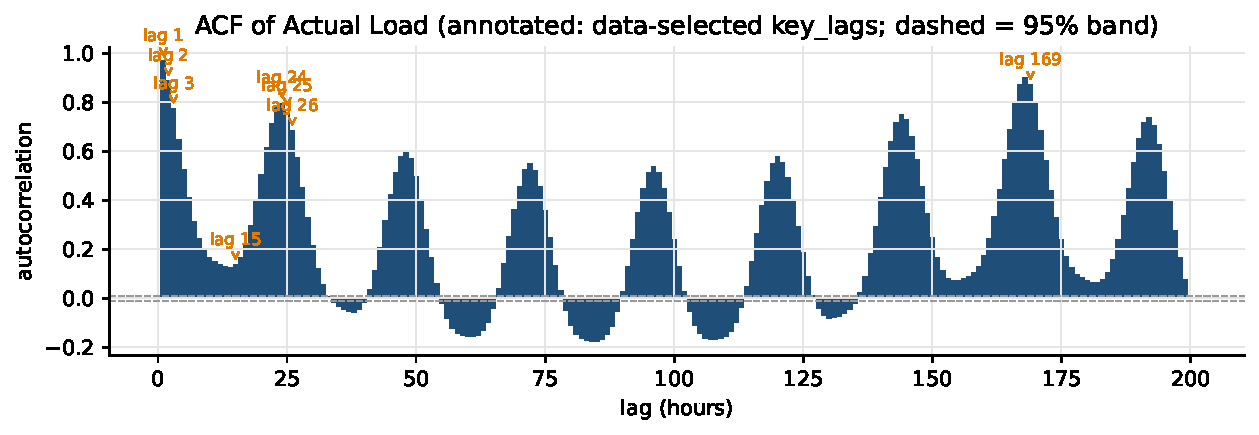
\includegraphics[keepaspectratio]{14_team_4_submission_files/figure-pdf/fig-team4-acf-output-2.pdf}}

}

\caption{\label{fig-team4-acf}Autocorrelation of the hourly
\texttt{Actual\ Load} up to lag 200, with the 95\% white-noise
significance band (±1.96/√N, dashed grey). The annotated
\texttt{key\_lags} are chosen dynamically --- the significant lags with
the largest \emph{partial} autocorrelation --- and are passed to
\texttt{ConfigEntsoe(lags\_consider=...)}. SpotOptim still selects the
model's final lags (Section~\ref{sec-team4-config}).}

\end{figure}%

\subsection{\texorpdfstring{Advanced
\texttt{ConfigEntsoe}}{Advanced ConfigEntsoe}}\label{sec-team4-config}

Each change relative to Section~\ref{sec-live-config} has a one-line
rationale:

\begin{itemize}
\tightlist
\item
  All five seasonal periods --- captures multi-scale seasonality the
  recursive LGBM cannot recover from hourly lags alone.
\item
  Data-selected lags --- the PACF-significant lags from 1 (typically
  hourly 1--3, daily \textasciitilde24, weekly \textasciitilde168), not
  a fixed set.
\item
  \texttt{include\_weather\_windows=True} --- temperature is the
  dominant load driver below \textasciitilde5 °C and above
  \textasciitilde15 °C.
\item
  \texttt{include\_holiday\_features=True} --- DE/NW public holidays
  shift weekday load by 20--30 \%.
\item
  \texttt{poly\_features\_degree=2} --- bilinear weather × calendar
  interactions, capped at \texttt{max\_poly\_features=10} (top ten by
  mutual information) so the feature space stays compact.
\item
  \texttt{n\_trials\_spotoptim=6}, \texttt{n\_initial\_spotoptim=5},
  \texttt{number\_folds=10} --- a deliberately small search budget that
  keeps the live render fast; raise it for a more thorough tuning run.
\end{itemize}

\protect\phantomsection\label{team4-config}
\begin{Shaded}
\begin{Highlighting}[]
\NormalTok{TRAIN\_SIZE }\OperatorTok{=}\NormalTok{ pd.Timedelta(days}\OperatorTok{=}\DecValTok{365} \OperatorTok{*} \DecValTok{3}\NormalTok{)}
\NormalTok{PREDICT\_SIZE }\OperatorTok{=} \DecValTok{24}
\NormalTok{REFIT\_SIZE }\OperatorTok{=} \DecValTok{7}
\NormalTok{NUMBER\_FOLDS }\OperatorTok{=} \DecValTok{10}
\NormalTok{DELTA\_VAL }\OperatorTok{=}\NormalTok{ pd.Timedelta(hours}\OperatorTok{=}\NormalTok{PREDICT\_SIZE }\OperatorTok{*}\NormalTok{ REFIT\_SIZE }\OperatorTok{*}\NormalTok{ NUMBER\_FOLDS)}
\CommentTok{\# Gap{-}penalty zone (hours) for weighted imputation, decoupled from the}
\CommentTok{\# rolling{-}feature \textasciigrave{}window\_size\textasciigrave{} (default 72). A narrower zone reduces the}
\CommentTok{\# "all sample weights zero {-}\textgreater{} uniform weighting" warning on short CV folds.}
\NormalTok{IMPUTATION\_WINDOW\_SIZE }\OperatorTok{=} \DecValTok{24}

\NormalTok{ADVANCED\_PERIODS }\OperatorTok{=}\NormalTok{ [}
\NormalTok{    Period(name}\OperatorTok{=}\StringTok{"daily"}\NormalTok{,     n\_periods}\OperatorTok{=}\DecValTok{12}\NormalTok{, column}\OperatorTok{=}\StringTok{"hour"}\NormalTok{,      input\_range}\OperatorTok{=}\NormalTok{(}\DecValTok{1}\NormalTok{, }\DecValTok{24}\NormalTok{)),}
\NormalTok{    Period(name}\OperatorTok{=}\StringTok{"weekly"}\NormalTok{,    n\_periods}\OperatorTok{=}\DecValTok{7}\NormalTok{,  column}\OperatorTok{=}\StringTok{"dayofweek"}\NormalTok{, input\_range}\OperatorTok{=}\NormalTok{(}\DecValTok{0}\NormalTok{, }\DecValTok{6}\NormalTok{)),}
\NormalTok{    Period(name}\OperatorTok{=}\StringTok{"monthly"}\NormalTok{,   n\_periods}\OperatorTok{=}\DecValTok{12}\NormalTok{, column}\OperatorTok{=}\StringTok{"month"}\NormalTok{,     input\_range}\OperatorTok{=}\NormalTok{(}\DecValTok{1}\NormalTok{, }\DecValTok{12}\NormalTok{)),}
\NormalTok{    Period(name}\OperatorTok{=}\StringTok{"quarterly"}\NormalTok{, n\_periods}\OperatorTok{=}\DecValTok{4}\NormalTok{,  column}\OperatorTok{=}\StringTok{"quarter"}\NormalTok{,   input\_range}\OperatorTok{=}\NormalTok{(}\DecValTok{1}\NormalTok{, }\DecValTok{4}\NormalTok{)),}
\NormalTok{    Period(name}\OperatorTok{=}\StringTok{"yearly"}\NormalTok{,    n\_periods}\OperatorTok{=}\DecValTok{12}\NormalTok{, column}\OperatorTok{=}\StringTok{"dayofyear"}\NormalTok{, input\_range}\OperatorTok{=}\NormalTok{(}\DecValTok{1}\NormalTok{, }\DecValTok{365}\NormalTok{)),}
\NormalTok{]}

\NormalTok{team4\_config }\OperatorTok{=}\NormalTok{ ConfigEntsoe(}
\NormalTok{    country\_code}\OperatorTok{=}\StringTok{"DE"}\NormalTok{,}
\NormalTok{    data\_filename}\OperatorTok{=}\StringTok{"interim/energy\_load.csv"}\NormalTok{,}
\NormalTok{    targets}\OperatorTok{=}\NormalTok{[}\StringTok{"Actual Load"}\NormalTok{],}
\NormalTok{    agg\_weights}\OperatorTok{=}\NormalTok{[}\FloatTok{1.0}\NormalTok{],}
\NormalTok{    bounds}\OperatorTok{=}\VariableTok{None}\NormalTok{,}
\NormalTok{    data\_loader}\OperatorTok{=}\NormalTok{entsoe\_data\_loader,}
\NormalTok{    test\_data\_loader}\OperatorTok{=}\NormalTok{entsoe\_test\_data\_loader,}
\NormalTok{    forecaster\_factory}\OperatorTok{=}\NormalTok{entsoe\_lgbm\_factory,}
\NormalTok{    periods}\OperatorTok{=}\NormalTok{ADVANCED\_PERIODS,}
\NormalTok{    lags\_consider}\OperatorTok{=}\NormalTok{key\_lags,}
\NormalTok{    train\_size}\OperatorTok{=}\NormalTok{TRAIN\_SIZE,}
\NormalTok{    end\_train\_default}\OperatorTok{=}\NormalTok{LAST\_FULL\_HOUR.isoformat(),}
\NormalTok{    delta\_val}\OperatorTok{=}\NormalTok{DELTA\_VAL,}
\NormalTok{    predict\_size}\OperatorTok{=}\NormalTok{LIVE\_N\_STEPS,}
\NormalTok{    cv\_block\_size}\OperatorTok{=}\NormalTok{PREDICT\_SIZE,}
\NormalTok{    refit\_size}\OperatorTok{=}\NormalTok{REFIT\_SIZE,}
\NormalTok{    number\_folds}\OperatorTok{=}\NormalTok{NUMBER\_FOLDS,}
\NormalTok{    imputation\_window\_size}\OperatorTok{=}\NormalTok{IMPUTATION\_WINDOW\_SIZE,}
\NormalTok{    n\_trials\_optuna}\OperatorTok{=}\DecValTok{15}\NormalTok{,}
\NormalTok{    n\_trials\_spotoptim}\OperatorTok{=}\DecValTok{30}\NormalTok{,}
\NormalTok{    n\_initial\_spotoptim}\OperatorTok{=}\DecValTok{10}\NormalTok{,}
\NormalTok{    warm\_start\_lags}\OperatorTok{=}\VariableTok{True}\NormalTok{,}
\NormalTok{    include\_weather\_windows}\OperatorTok{=}\VariableTok{True}\NormalTok{,}
\NormalTok{    include\_holiday\_features}\OperatorTok{=}\VariableTok{True}\NormalTok{,}
\NormalTok{    poly\_features\_degree}\OperatorTok{=}\DecValTok{2}\NormalTok{,}
\NormalTok{    max\_poly\_features}\OperatorTok{=}\DecValTok{10}\NormalTok{,}
\NormalTok{    state}\OperatorTok{=}\StringTok{"NW"}\NormalTok{,}
\NormalTok{    random\_state}\OperatorTok{=}\DecValTok{42}\NormalTok{,}
\NormalTok{    on\_weather\_failure}\OperatorTok{=}\StringTok{"skip"}\NormalTok{,}
\NormalTok{)}
\NormalTok{team4\_config.data\_frame\_name }\OperatorTok{=} \StringTok{"ddmo{-}live{-}team4"}
\BuiltInTok{print}\NormalTok{(}\StringTok{"team4\_config ready:"}\NormalTok{, team4\_config.data\_frame\_name,}
      \StringTok{"| predict\_size="}\NormalTok{, team4\_config.predict\_size,}
      \StringTok{"| n\_trials\_spotoptim="}\NormalTok{, team4\_config.n\_trials\_spotoptim,}
      \StringTok{"| number\_folds="}\NormalTok{, team4\_config.number\_folds)}
\end{Highlighting}
\end{Shaded}

\begin{verbatim}
team4_config ready: ddmo-live-team4 | predict_size= 29 | n_trials_spotoptim= 30 | number_folds= 10
\end{verbatim}

\subsubsection{What each constant and argument
means}\label{what-each-constant-and-argument-means}

The cell defines two things: a handful of local constants that fix the
cross-validation geometry and the feature menu, and the
\texttt{ConfigEntsoe} object that records every choice the pipeline
reads. The value shown for each item is the one used here.

Local constants --- the cross-validation geometry:

\begin{itemize}
\tightlist
\item
  \texttt{TRAIN\_SIZE} --- length of the rolling training window, a
  \texttt{pd.Timedelta}. Here \texttt{pd.Timedelta(days=365\ *\ 3)},
  i.e.~three years. Example: a fold whose \texttt{end\_train} is
  \texttt{2026-05-20\ 23:00} reaches back to roughly
  \texttt{2023-05-21\ 00:00}.
\item
  \texttt{PREDICT\_SIZE} --- length of one forecast block in hours.
  \texttt{24} is one day. It feeds \texttt{DELTA\_VAL} only; the
  config's live horizon is \texttt{predict\_size=LIVE\_N\_STEPS}
  (below), not this fixed \texttt{24}.
\item
  \texttt{REFIT\_SIZE} --- spacing, in days, at which the model is refit
  while back-testing. \texttt{7} means a weekly refit.
\item
  \texttt{NUMBER\_FOLDS} --- number of time-ordered cross-validation
  folds. \texttt{10}.
\item
  \texttt{DELTA\_VAL} --- total validation span reserved for the rolling
  CV,
  \texttt{pd.Timedelta(hours=PREDICT\_SIZE\ *\ REFIT\_SIZE\ *\ NUMBER\_FOLDS)}
  = \texttt{24\ ×\ 7\ ×\ 10\ =\ 1680} h = 70 days. The most recent 70
  days of history are held out for evaluation. This constant is
  explained in detail in Section~\ref{sec-cross-validation-geometry}.
\item
  \texttt{ADVANCED\_PERIODS} --- a list of \texttt{Period} cyclical
  encodings, one per seasonal scale. Each
  \texttt{Period(name,\ n\_periods,\ column,\ input\_range)} reads
  \texttt{column} off the timestamp, treats its values as living on
  \texttt{input\_range}, and encodes them with \texttt{n\_periods}
  smooth basis functions. Example:
  \texttt{Period("daily",\ 12,\ "hour",\ (1,\ 24))} turns the
  hour-of-day into 12 daily encodings;
  \texttt{Period("weekly",\ 7,\ "dayofweek",\ (0,\ 6))} gives a
  seven-way day-of-week encoding.
\end{itemize}

(The autoregressive lags are no longer a constant here:
\texttt{key\_lags} is selected from the data in 1 and passed straight to
\texttt{lags\_consider} below.)

\texttt{ConfigEntsoe} --- identity and data source:

\begin{itemize}
\tightlist
\item
  \texttt{country\_code="DE"} --- ISO 3166-1 alpha-2 code; selects both
  the ENTSO-E query and the national holiday calendar.
\item
  \texttt{data\_filename="interim/energy\_load.csv"} --- path, under the
  data home, of the merged interim frame to read (the file profiled in
  Section~\ref{sec-team4-interim}).
\item
  \texttt{targets={[}"Actual\ Load"{]}} --- the column(s) to forecast;
  one target here.
\item
  \texttt{agg\_weights={[}1.0{]}} --- per-target weight used when
  several targets are aggregated into one score; with a single target it
  is \texttt{1.0}.
\item
  \texttt{bounds=None} --- per-target outlier limits, left unset here on
  purpose. A fixed pair like \texttt{±1e9} MW would never flag anything;
  instead the bounds are \emph{derived from the long load history}
  (relaxed \texttt{median\ ±\ 5·IQR}, lower floored at 0 MW) and
  assigned just before detection in Section~\ref{sec-team4-outliers}.
  These hard bounds are the only step that marks anomalies; the
  IsolationForest pass is report-only logging (see
  Section~\ref{sec-team4-outliers}).
\end{itemize}

\texttt{ConfigEntsoe} --- pipeline wiring (callables):

\begin{itemize}
\tightlist
\item
  \texttt{data\_loader=entsoe\_data\_loader} --- function
  \texttt{loader(config)} that returns the training DataFrame; invoked
  by \texttt{prepare\_data()}.
\item
  \texttt{test\_data\_loader=entsoe\_test\_data\_loader} --- function
  returning ground-truth values for the horizon, used to populate
  \texttt{test\_actual} and \texttt{metrics\_future} when they exist.
\item
  \texttt{forecaster\_factory=entsoe\_lgbm\_factory} --- factory that
  builds the LightGBM recursive forecaster the search then tunes.
\end{itemize}

\texttt{ConfigEntsoe} --- features:

\begin{itemize}
\tightlist
\item
  \texttt{periods=ADVANCED\_PERIODS} --- wire in the seasonal encodings
  above.
\item
  \texttt{lags\_consider=key\_lags} --- the data-selected candidate lags
  computed in

  \begin{enumerate}
  \def\labelenumi{\arabic{enumi}.}
  \tightlist
  \item
    Paired with \texttt{warm\_start\_lags=True} (below), this list is
    injected as a candidate in the tuner's lag search and seeded as its
    first evaluation; see the note after this list for exactly how it is
    consumed.
  \end{enumerate}
\item
  \texttt{include\_weather\_windows=True} --- add rolling weather-window
  features.
\item
  \texttt{include\_holiday\_features=True} --- add public-holiday
  indicators, regionalised by \texttt{state}.
\item
  \texttt{poly\_features\_degree=2} --- generate pairwise bilinear
  interaction terms (\texttt{1} would disable interactions).
\item
  \texttt{max\_poly\_features=10} --- keep only the ten most informative
  interaction columns, ranked by mutual information with the target.
\item
  \texttt{state="NW"} --- the German subdivision code (North
  Rhine-Westphalia) driving the regional holiday calendar.
\end{itemize}

\begin{tcolorbox}[enhanced jigsaw, arc=.35mm, bottomrule=.15mm, bottomtitle=1mm, breakable, colback=white, colbacktitle=quarto-callout-note-color!10!white, colframe=quarto-callout-note-color-frame, coltitle=black, left=2mm, leftrule=.75mm, opacityback=0, opacitybacktitle=0.6, rightrule=.15mm, title=\textcolor{quarto-callout-note-color}{\faInfo}\hspace{0.5em}{Where \texttt{key\_lags} is used --- and who really picks the lags}, titlerule=0mm, toprule=.15mm, toptitle=1mm]

A natural question is whether \texttt{lags\_consider=key\_lags} fixes
the lags the model forecasts on, or whether the tuner decides. In the
tuned \texttt{spotoptim} run this chapter performs
(\texttt{MultiTask(team4\_config,\ task="spotoptim")}), the tuner still
chooses the winner, but with \texttt{warm\_start\_lags=True} the
data-selected list now genuinely competes. Three steps consume it:

\begin{enumerate}
\def\labelenumi{\arabic{enumi}.}
\tightlist
\item
  The forecaster factory \texttt{entsoe\_lgbm\_factory}
  (\texttt{spotforecast2/multitask/factories.py}) builds the
  \emph{initial} forecaster with
  \texttt{lags=config.lags\_consider{[}-1{]}} --- only the largest
  entry. With the data-selected \texttt{key\_lags} (whose maximum is the
  weekly lag, around \texttt{168}), \texttt{initialize\_lags} expands
  that maximum to the full contiguous range \texttt{1…max}, not the
  individual selected lags.
\item
  SpotOptim treats the lag configuration as a categorical hyperparameter
  and searches a candidate set. By default that set is hardcoded
  (\texttt{\_default\_spotoptim\_search\_space} in
  \texttt{spotforecast2/multitask/search\_spaces.py} ---
  e.g.~\texttt{"24"}, \texttt{"{[}1,\ 2,\ 24,\ 48{]}"},
  \texttt{"{[}1,\ 2,\ 11,\ 12,\ 23,\ 24,\ 167,\ 168{]}"}). With
  \texttt{warm\_start\_lags=True}, \texttt{SpotOptimStrategy}
  \emph{prepends} \texttt{str(key\_lags)} to that list, so the
  PACF-selected lags become a real, selectable candidate.
\item
  The same flag seeds the surrogate search:
  \texttt{build\_warm\_start\_x0} constructs the optimizer's first
  evaluation point at \texttt{key\_lags} (combined with the factory's
  estimator defaults) and passes it as SpotOptim's \texttt{x0}, so the
  seeded configuration is guaranteed to be evaluated rather than left to
  chance in the random initial design. The winner is applied with
  \texttt{set\_lags}, logged as ``Best lags'', and inspectable via
  exercise 3.
\end{enumerate}

A consequence worth flagging: \texttt{initialize\_lags} expands an
\emph{integer} candidate to the contiguous range \texttt{1…max}, but
leaves a \emph{list} candidate untouched. So when the logged ``Best
lags'' come back gapless (e.g.~\texttt{1…24}), it means the integer
candidate \texttt{"24"} won the back-test --- not that the search cannot
carry gaps. The candidate set above includes genuine non-contiguous sets
such as \texttt{{[}1,\ 2,\ 11,\ 12,\ 23,\ 24,\ 167,\ 168{]}}, and the
winning lags are free to be one of them; the weekly lag survives in the
search whether or not it wins.

So under \texttt{warm\_start\_lags=True} the ACF analysis in 1 no longer
only \emph{motivates} candidate lags --- it injects them into the search
and seeds the optimizer with them, while the tuner still has the final
say among all candidates. With \texttt{warm\_start\_lags=False} (the
default), \texttt{lags\_consider} reverts to its passive role: only its
maximum (\texttt{lags\_consider{[}-1{]}}) sizes the pre-tuning
forecaster and the minimum history the back-test reserves, and the tuner
picks from the hardcoded set alone.

\end{tcolorbox}

\texttt{ConfigEntsoe} --- training window, horizon, refit:

\begin{itemize}
\tightlist
\item
  \texttt{train\_size=TRAIN\_SIZE}, \texttt{delta\_val=DELTA\_VAL},
  \texttt{refit\_size=REFIT\_SIZE}, \texttt{number\_folds=NUMBER\_FOLDS}
  --- hand the CV geometry above to the config.
\item
  \texttt{end\_train\_default=LAST\_FULL\_HOUR.isoformat()} --- ISO
  timestamp anchoring the end of training: the last full hour of
  published actuals (Section~\ref{sec-team4-cutoff}). Example:
  \texttt{"2026-05-20T23:00:00+00:00"}.
\item
  \texttt{predict\_size=LIVE\_N\_STEPS} --- the live horizon in hours,
  i.e.~the recursive bridge from \texttt{end\_train} through tomorrow
  23:00 UTC, which is longer than the fixed \texttt{PREDICT\_SIZE=24}.
\item
  \texttt{cv\_block\_size=PREDICT\_SIZE} --- the cross-validation
  test-block width (24 h), fixed and decoupled from the render-dependent
  live \texttt{predict\_size}. Leaving it unset would make the CV
  inherit \texttt{predict\_size=LIVE\_N\_STEPS}; pinning it at 24 keeps
  the fold geometry stable across renders
  (Section~\ref{sec-cross-validation-geometry}).
\end{itemize}

\texttt{ConfigEntsoe} --- search budget and reproducibility:

\begin{itemize}
\tightlist
\item
  \texttt{n\_trials\_optuna=15} --- Optuna Bayesian-search trial budget.
\item
  \texttt{n\_trials\_spotoptim=6} --- SpotOptim surrogate-search trial
  budget.
\item
  \texttt{n\_initial\_spotoptim=5} --- SpotOptim initial random
  evaluations before the surrogate model takes over.
\item
  \texttt{warm\_start\_lags=True} --- inject \texttt{key\_lags} as a
  candidate lag set and seed the surrogate search's first evaluation
  with it (see the note above).
\item
  \texttt{random\_state=42} --- RNG seed fixing tuning and model
  randomness, so the render is reproducible (CR-2).
\item
  \texttt{on\_weather\_failure="skip"} --- if the Open-Meteo fetch
  fails, log a warning and continue with empty weather features rather
  than abort; \texttt{"raise"} (the default) would fail loud instead.
\end{itemize}

Finally, the post-construction assignment
\texttt{team4\_config.data\_frame\_name\ =\ "ddmo-live-team4"} names the
cache subdirectory, the saved-model files, and the per-dataset log for
this run.

The \texttt{MultiTask} orchestrator runs the full pipeline in one call,
but a safety-critical forecaster is only trustworthy if its inputs are
auditable. The next six subsections run the pipeline one method at a
time and inspect the data each step produces --- endogenous series,
curation, imputation, exogenous features, the tuned forecast, and the
feature attributions. Each method mutates \texttt{team4\_mt} in place,
so the cells must run top to bottom.

\subsection{Cross-validation geometry
recap}\label{sec-cross-validation-geometry}

The four constants defined at the top of Section~\ref{sec-team4-config}
--- \texttt{PREDICT\_SIZE}, \texttt{REFIT\_SIZE},
\texttt{NUMBER\_FOLDS}, and the \texttt{DELTA\_VAL} they combine into
--- do one job: they fix the \emph{cross-validation geometry} that
SpotOptim scores every candidate model against. The config explainer
above quoted the result (``the most recent 70 days are held out''); this
section derives that number from scratch and shows exactly how the
rolling back-test that produces SpotOptim's objective is laid out. It is
self-contained --- it reuses the chronological-split idea of
Chapter~\ref{sec-split} and the rolling-origin back-test of
Chapter~\ref{sec-backtest}, but every term needed is defined here.

\subsubsection{Definitions}\label{definitions}

The pipeline reasons about one contiguous, hourly, gap-free load series.
The following terms pin down how that series is carved up for tuning.

\begin{description}
\tightlist
\item[Training series]
the full hourly \texttt{Actual\ Load} the tuner is allowed to look at.
It runs from \texttt{start\_train} to \texttt{end\_train}.
\item[\texttt{end\_train}]
the last timestamp the model may train on --- here
\texttt{LAST\_FULL\_HOUR}, the last full hour of published actuals
(Section~\ref{sec-team4-cutoff}). Everything after it is the live
forecast, never part of tuning.
\item[\texttt{train\_size}]
the length of the training series as a duration.
\texttt{start\_train\ =\ end\_train\ −\ train\_size}. Here three years.
\item[\texttt{predict\_size}]
the \emph{live} forecast horizon --- how many hours the model is asked
to forecast forward in production. The live config sets it to
\texttt{LIVE\_N\_STEPS} (Section~\ref{sec-team4-cutoff}), the recursive
bridge to tomorrow 23:00, so it is render-dependent (≈ 32). It does
\emph{not} set the cross-validation block; that is
\texttt{cv\_block\_size}.
\item[\texttt{cv\_block\_size}]
the width of each cross-validation test block, in hours --- the horizon
the folds actually score. The config sets it to
\texttt{PREDICT\_SIZE\ =\ 24} (one day), fixed and independent of the
render-dependent \texttt{predict\_size}. Decoupling the two is
deliberate: the CV scores a stable 24-hour-ahead block while the live
forecast still runs out to \texttt{LIVE\_N\_STEPS}. (When
\texttt{cv\_block\_size} is left unset it falls back to
\texttt{predict\_size} --- the behaviour chapters 02--11 rely on, where
the two coincide at 24.)
\item[\texttt{delta\_val}]
the validation span: the stretch of the most recent history reserved for
evaluation and withheld from the model's training. It is computed, not
chosen directly --- see below.
\item[\texttt{end\_cv}]
the cross-validation training cutoff,
\texttt{end\_cv\ =\ end\_train\ −\ delta\_val}. The model is trained on
\texttt{{[}start\_train,\ end\_cv{]}} and validated on
\texttt{(end\_cv,\ end\_train{]}}.
\item[Fold]
one (train, test) pair. Every fold trains on data ending at or before
its test block and predicts the next \texttt{cv\_block\_size} hours ---
so a fold never peeks at its own future, the discipline introduced in
Chapter~\ref{sec-split}.
\item[Fold stride]
how far the test block advances between consecutive folds. Here it
equals \texttt{cv\_block\_size\ =\ 24}, so the folds are back-to-back
and non-overlapping: together they tile the whole validation span
exactly once.
\item[Rolling-origin back-test]
the procedure (Chapter~\ref{sec-backtest}) that slides the forecast
origin forward one stride at a time across the validation span,
collecting a forecast at each step. With \texttt{refit=False} the
forecaster is fit \emph{once} on \texttt{{[}start\_train,\ end\_cv{]}}
and then reused to produce every fold's forecast --- fast, and a
deterministic choice (CR-2).
\item[Mean absolute error (MAE)]
the score. The fold forecasts are pooled into one vector \(\hat{y}\),
compared with the matching actuals \(y\), and averaged:
\(\text{MAE} = \tfrac{1}{n}\sum_{t=1}^{n}\lvert y_t - \hat{y}_t\rvert\).
This single number, over all validation hours, is what SpotOptim
minimises.
\end{description}

\subsubsection{\texorpdfstring{Computing
\texttt{DELTA\_VAL}}{Computing DELTA\_VAL}}\label{computing-delta_val}

\texttt{DELTA\_VAL} is the product of the other three constants, read as
hours:

\[
\texttt{DELTA\_VAL}
  = \underbrace{\texttt{PREDICT\_SIZE}}_{24\ \text{h/fold}}
  \times \underbrace{\texttt{REFIT\_SIZE}}_{7}
  \times \underbrace{\texttt{NUMBER\_FOLDS}}_{10}
  = 24 \times 7 \times 10 = 1680\ \text{h} = 70\ \text{days}.
\]

This span is then sliced off the \emph{tail} of the training series.
With \texttt{end\_cv\ =\ end\_train\ −\ delta\_val}, the series splits
cleanly into a training part and a validation part whose lengths add up
to \texttt{train\_size}:

\[
\underbrace{\texttt{train\_size}}_{3\ \text{yr}\,=\,26280\ \text{h}}
  = \underbrace{(\texttt{train\_size} - \texttt{delta\_val})}_{\text{CV training window}}
  + \underbrace{\texttt{delta\_val}}_{\text{validation span}}
  = 24600\ \text{h} + 1680\ \text{h}.
\]

The fold count then falls straight out of the geometry. The folds are
non-overlapping blocks of \texttt{cv\_block\_size\ =\ 24} hours that
tile the validation span, so their number is

\[
\#\text{folds}
  = \frac{\texttt{delta\_val}}{\texttt{cv\_block\_size}}
  = \frac{1680}{24}
  = \texttt{REFIT\_SIZE} \times \texttt{NUMBER\_FOLDS}
  = 7 \times 10 = 70,
\]

and the total validation hours scored is \(70 \times 24 = 1680 =
\texttt{delta\_val}\). The \texttt{70/70} progress bars at
Section~\ref{sec-team4-run} are exactly this count, the same for every
render. The clean identity holds \emph{because} we set
\texttt{cv\_block\_size\ =\ PREDICT\_SIZE}. Had the CV instead inherited
the live \texttt{predict\_size\ =\ LIVE\_N\_STEPS} (≈ 32 h) --- as it
did before the \texttt{cv\_block\_size} field existed --- the block
would tile the span into \texttt{⌈1680\ /\ 32⌉\ =\ 53} folds, and the
count would drift render to render with the feed's freshness
(Section~\ref{sec-team4-cutoff}). Decoupling the CV block from the live
horizon is exactly what \texttt{cv\_block\_size} buys.

A note on the names, so the arithmetic is not mistaken for behaviour the
code does not have. In \emph{this} cross-validation the model is fit
once and reused (\texttt{refit=False}), so \texttt{REFIT\_SIZE} does not
trigger any refitting --- it is one of two factors whose product, with
\texttt{PREDICT\_SIZE}, sizes the held-out span. Likewise
\texttt{NUMBER\_FOLDS} enters only through that product; because we set
\texttt{cv\_block\_size\ =\ PREDICT\_SIZE}, the real fold count is the
70 derived above, not 10. The constants are a convenient way to
\emph{spell} a 70-day window as ``ten weekly blocks of daily
forecasts'', not a description of a ten-fold refit loop. (Internally
\texttt{cv\_ts} in \texttt{spotforecast2} reads \texttt{cv\_block\_size}
--- falling back to \texttt{predict\_size} when it is unset --- sets
\texttt{end\_cv\ =\ end\_train\ −\ delta\_val}, and returns a
\texttt{TimeSeriesFold(steps=cv\_block\_size,\ refit=False,\ allow\_incomplete\_fold=True)}
--- the same \texttt{TimeSeriesFold} machinery used in
Chapter~\ref{sec-backtest}.)

\subsubsection{A toy example you can check by
hand}\label{a-toy-example-you-can-check-by-hand}

The real case (dozens of folds) is hard to draw, so first shrink every
constant. Take \texttt{predict\_size\ =\ 2}, \texttt{refit\_size\ =\ 2},
\texttt{number\_folds\ =\ 3}, and a training series of
\texttt{train\_size\ =\ 30} time units. Then

\[
\texttt{delta\_val} = 2 \times 2 \times 3 = 12,\quad
\text{CV training window} = 30 - 12 = 18,\quad
\#\text{folds} = \tfrac{12}{2} = 6.
\]

Index the series \(0,1,\dots,29\). Training is the fixed block
\([0, 18)\); the six test blocks tile the last twelve positions, each
two wide:

{\def\LTcaptype{none} % do not increment counter
\begin{longtable}[]{@{}ccc@{}}
\toprule\noalign{}
fold & trains on & tests on \\
\midrule\noalign{}
\endhead
\bottomrule\noalign{}
\endlastfoot
1 & {[}0, 18) & {[}18, 20) \\
2 & {[}0, 18) & {[}20, 22) \\
3 & {[}0, 18) & {[}22, 24) \\
4 & {[}0, 18) & {[}24, 26) \\
5 & {[}0, 18) & {[}26, 28) \\
6 & {[}0, 18) & {[}28, 30) \\
\end{longtable}
}

The model is fit once on \([0,18)\), makes six successive 2-step
forecasts that march across \([18,30)\), and the MAE is taken over all
\(6 \times 2 = 12\) predicted positions. In this toy the block
(\texttt{cv\_block\_size\ =\ 2}) equals the unit that sizes
\texttt{delta\_val}, so the fold count is the clean
\texttt{delta\_val\ /\ cv\_block\_size\ =\ 6}. The schematic below draws
exactly this layout; the real configuration is the same picture with 70
daily (24-hour) blocks instead of six 2-step ones --- the live
\texttt{predict\_size\ =\ LIVE\_N\_STEPS} plays no part in the CV
geometry, only in the production forecast.

\begin{Shaded}
\begin{Highlighting}[]
\ImportTok{import}\NormalTok{ matplotlib.pyplot }\ImportTok{as}\NormalTok{ plt}
\ImportTok{import}\NormalTok{ matplotlib.patches }\ImportTok{as}\NormalTok{ mpatches}

\CommentTok{\# Toy constants (small enough to draw every block); the real run scales these}
\CommentTok{\# to PREDICT\_SIZE=24, REFIT\_SIZE=7, NUMBER\_FOLDS=10 {-}\textgreater{} 1680 h (70{-}day) span,}
\CommentTok{\# tiled into cv\_block\_size=24{-}h blocks {-}\textgreater{} 1680/24 = 70 folds (render{-}independent).}
\NormalTok{PS, RS, NF }\OperatorTok{=} \DecValTok{2}\NormalTok{, }\DecValTok{2}\NormalTok{, }\DecValTok{3}          \CommentTok{\# cv\_block\_size, refit\_size, number\_folds}
\NormalTok{TRAIN }\OperatorTok{=} \DecValTok{30}                    \CommentTok{\# train\_size, in the same time units as the folds}
\NormalTok{DV }\OperatorTok{=}\NormalTok{ PS }\OperatorTok{*}\NormalTok{ RS }\OperatorTok{*}\NormalTok{ NF             }\CommentTok{\# delta\_val = 12}
\NormalTok{CVT }\OperatorTok{=}\NormalTok{ TRAIN }\OperatorTok{{-}}\NormalTok{ DV              }\CommentTok{\# CV training window = 18}
\NormalTok{NFOLDS }\OperatorTok{=}\NormalTok{ DV }\OperatorTok{//}\NormalTok{ PS             }\CommentTok{\# number of folds = 6}

\NormalTok{BLUE, ORANGE, GREY, GRID }\OperatorTok{=} \StringTok{"\#1F4E79"}\NormalTok{, }\StringTok{"\#E07B00"}\NormalTok{, }\StringTok{"\#999999"}\NormalTok{, }\StringTok{"\#E5E5E5"}

\NormalTok{fig, (axA, axB) }\OperatorTok{=}\NormalTok{ plt.subplots(}
    \DecValTok{2}\NormalTok{, }\DecValTok{1}\NormalTok{, figsize}\OperatorTok{=}\NormalTok{(}\FloatTok{8.5}\NormalTok{, }\FloatTok{4.6}\NormalTok{), gridspec\_kw}\OperatorTok{=}\NormalTok{\{}\StringTok{"height\_ratios"}\NormalTok{: [}\FloatTok{1.0}\NormalTok{, }\FloatTok{1.5}\NormalTok{]\}}
\NormalTok{)}

\CommentTok{\# {-}{-}{-} Panel A: the split of the training series {-}{-}{-}{-}{-}{-}{-}{-}{-}{-}{-}{-}{-}{-}{-}{-}{-}{-}{-}{-}{-}{-}{-}{-}{-}{-}{-}{-}{-}{-}{-}{-}}
\NormalTok{axA.add\_patch(mpatches.Rectangle((}\DecValTok{0}\NormalTok{, }\DecValTok{0}\NormalTok{), CVT, }\DecValTok{1}\NormalTok{, facecolor}\OperatorTok{=}\NormalTok{BLUE,}
\NormalTok{                                 edgecolor}\OperatorTok{=}\StringTok{"white"}\NormalTok{, label}\OperatorTok{=}\StringTok{"CV training window"}\NormalTok{))}
\ControlFlowTok{for}\NormalTok{ k }\KeywordTok{in} \BuiltInTok{range}\NormalTok{(NFOLDS):}
\NormalTok{    axA.add\_patch(mpatches.Rectangle((CVT }\OperatorTok{+}\NormalTok{ k }\OperatorTok{*}\NormalTok{ PS, }\DecValTok{0}\NormalTok{), PS, }\DecValTok{1}\NormalTok{, facecolor}\OperatorTok{=}\NormalTok{ORANGE,}
\NormalTok{                                     edgecolor}\OperatorTok{=}\StringTok{"white"}\NormalTok{))}
\CommentTok{\# marker lines + labels for the three anchors}
\ControlFlowTok{for}\NormalTok{ x, lab }\KeywordTok{in}\NormalTok{ [(}\DecValTok{0}\NormalTok{, }\StringTok{"start\_train"}\NormalTok{), (CVT, }\StringTok{"end\_cv"}\NormalTok{), (TRAIN, }\StringTok{"end\_train"}\NormalTok{)]:}
\NormalTok{    axA.axvline(x, color}\OperatorTok{=}\StringTok{"\#555555"}\NormalTok{, lw}\OperatorTok{=}\FloatTok{0.7}\NormalTok{, ls}\OperatorTok{=}\StringTok{"{-}{-}"}\NormalTok{)}
\NormalTok{    axA.text(x, }\OperatorTok{{-}}\FloatTok{0.35}\NormalTok{, lab, ha}\OperatorTok{=}\StringTok{"center"}\NormalTok{, va}\OperatorTok{=}\StringTok{"top"}\NormalTok{, fontsize}\OperatorTok{=}\DecValTok{8}\NormalTok{, color}\OperatorTok{=}\StringTok{"\#333333"}\NormalTok{)}
\CommentTok{\# delta\_val span annotation}
\NormalTok{axA.annotate(}\StringTok{""}\NormalTok{, xy}\OperatorTok{=}\NormalTok{(CVT, }\FloatTok{1.35}\NormalTok{), xytext}\OperatorTok{=}\NormalTok{(TRAIN, }\FloatTok{1.35}\NormalTok{),}
\NormalTok{             arrowprops}\OperatorTok{=}\BuiltInTok{dict}\NormalTok{(arrowstyle}\OperatorTok{=}\StringTok{"\textless{}{-}\textgreater{}"}\NormalTok{, color}\OperatorTok{=}\NormalTok{ORANGE, lw}\OperatorTok{=}\FloatTok{1.0}\NormalTok{))}
\NormalTok{axA.text((CVT }\OperatorTok{+}\NormalTok{ TRAIN) }\OperatorTok{/} \DecValTok{2}\NormalTok{, }\FloatTok{1.5}\NormalTok{, }\SpecialStringTok{f"delta\_val = }\SpecialCharTok{\{}\NormalTok{DV}\SpecialCharTok{\}}\SpecialStringTok{"}\NormalTok{, ha}\OperatorTok{=}\StringTok{"center"}\NormalTok{,}
\NormalTok{         fontsize}\OperatorTok{=}\DecValTok{8}\NormalTok{, color}\OperatorTok{=}\NormalTok{ORANGE)}
\CommentTok{\# one predict\_size block annotation}
\NormalTok{axA.annotate(}\StringTok{""}\NormalTok{, xy}\OperatorTok{=}\NormalTok{(CVT, }\FloatTok{1.12}\NormalTok{), xytext}\OperatorTok{=}\NormalTok{(CVT }\OperatorTok{+}\NormalTok{ PS, }\FloatTok{1.12}\NormalTok{),}
\NormalTok{             arrowprops}\OperatorTok{=}\BuiltInTok{dict}\NormalTok{(arrowstyle}\OperatorTok{=}\StringTok{"\textless{}{-}\textgreater{}"}\NormalTok{, color}\OperatorTok{=}\StringTok{"\#333333"}\NormalTok{, lw}\OperatorTok{=}\FloatTok{0.8}\NormalTok{))}
\NormalTok{axA.text(CVT }\OperatorTok{+}\NormalTok{ PS }\OperatorTok{/} \DecValTok{2}\NormalTok{, }\FloatTok{1.2}\NormalTok{, }\SpecialStringTok{f"predict\_size = }\SpecialCharTok{\{}\NormalTok{PS}\SpecialCharTok{\}}\SpecialStringTok{"}\NormalTok{, ha}\OperatorTok{=}\StringTok{"left"}\NormalTok{, fontsize}\OperatorTok{=}\DecValTok{7}\NormalTok{,}
\NormalTok{         color}\OperatorTok{=}\StringTok{"\#333333"}\NormalTok{)}
\NormalTok{axA.set\_xlim(}\OperatorTok{{-}}\FloatTok{1.5}\NormalTok{, TRAIN }\OperatorTok{+} \FloatTok{1.5}\NormalTok{)}
\NormalTok{axA.set\_ylim(}\OperatorTok{{-}}\FloatTok{0.9}\NormalTok{, }\FloatTok{1.8}\NormalTok{)}
\NormalTok{axA.set\_yticks([])}
\NormalTok{axA.set\_title(}\SpecialStringTok{f"Series split: train\_size }\SpecialCharTok{\{}\NormalTok{TRAIN}\SpecialCharTok{\}}\SpecialStringTok{ = CV{-}train }\SpecialCharTok{\{}\NormalTok{CVT}\SpecialCharTok{\}}\SpecialStringTok{ + delta\_val }\SpecialCharTok{\{}\NormalTok{DV}\SpecialCharTok{\}}\SpecialStringTok{"}
              \SpecialStringTok{f"   ({-}\textgreater{} }\SpecialCharTok{\{}\NormalTok{NFOLDS}\SpecialCharTok{\}}\SpecialStringTok{ folds; real run: 1680/24 = 70 folds over 70 days)"}\NormalTok{,}
\NormalTok{              fontsize}\OperatorTok{=}\DecValTok{9}\NormalTok{)}
\ControlFlowTok{for}\NormalTok{ s }\KeywordTok{in}\NormalTok{ (}\StringTok{"top"}\NormalTok{, }\StringTok{"right"}\NormalTok{, }\StringTok{"left"}\NormalTok{):}
\NormalTok{    axA.spines[s].set\_visible(}\VariableTok{False}\NormalTok{)}

\CommentTok{\# {-}{-}{-} Panel B: the rolling{-}origin folds, one per row {-}{-}{-}{-}{-}{-}{-}{-}{-}{-}{-}{-}{-}{-}{-}{-}{-}{-}{-}{-}{-}{-}{-}{-}{-}{-}{-}}
\ControlFlowTok{for}\NormalTok{ k }\KeywordTok{in} \BuiltInTok{range}\NormalTok{(NFOLDS):}
\NormalTok{    y }\OperatorTok{=}\NormalTok{ NFOLDS }\OperatorTok{{-}} \DecValTok{1} \OperatorTok{{-}}\NormalTok{ k                       }\CommentTok{\# fold 1 on top}
\NormalTok{    axB.add\_patch(mpatches.Rectangle((}\DecValTok{0}\NormalTok{, y }\OperatorTok{+} \FloatTok{0.1}\NormalTok{), CVT, }\FloatTok{0.8}\NormalTok{, facecolor}\OperatorTok{=}\NormalTok{BLUE,}
\NormalTok{                                     edgecolor}\OperatorTok{=}\StringTok{"white"}\NormalTok{))}
\NormalTok{    axB.add\_patch(mpatches.Rectangle((CVT }\OperatorTok{+}\NormalTok{ k }\OperatorTok{*}\NormalTok{ PS, y }\OperatorTok{+} \FloatTok{0.1}\NormalTok{), PS, }\FloatTok{0.8}\NormalTok{,}
\NormalTok{                                     facecolor}\OperatorTok{=}\NormalTok{ORANGE, edgecolor}\OperatorTok{=}\StringTok{"white"}\NormalTok{))}
\NormalTok{    axB.text(}\OperatorTok{{-}}\FloatTok{0.5}\NormalTok{, y }\OperatorTok{+} \FloatTok{0.5}\NormalTok{, }\SpecialStringTok{f"fold }\SpecialCharTok{\{}\NormalTok{k }\OperatorTok{+} \DecValTok{1}\SpecialCharTok{\}}\SpecialStringTok{"}\NormalTok{, ha}\OperatorTok{=}\StringTok{"right"}\NormalTok{, va}\OperatorTok{=}\StringTok{"center"}\NormalTok{, fontsize}\OperatorTok{=}\DecValTok{8}\NormalTok{)}
\NormalTok{axB.axvline(CVT, color}\OperatorTok{=}\StringTok{"\#555555"}\NormalTok{, lw}\OperatorTok{=}\FloatTok{0.7}\NormalTok{, ls}\OperatorTok{=}\StringTok{"{-}{-}"}\NormalTok{)}
\NormalTok{axB.text(CVT, }\OperatorTok{{-}}\FloatTok{0.4}\NormalTok{, }\StringTok{"end\_cv"}\NormalTok{, ha}\OperatorTok{=}\StringTok{"center"}\NormalTok{, va}\OperatorTok{=}\StringTok{"top"}\NormalTok{, fontsize}\OperatorTok{=}\DecValTok{8}\NormalTok{, color}\OperatorTok{=}\StringTok{"\#333333"}\NormalTok{)}
\NormalTok{axB.text(CVT }\OperatorTok{/} \DecValTok{2}\NormalTok{, NFOLDS }\OperatorTok{+} \FloatTok{0.25}\NormalTok{, }\StringTok{"fit once (refit=False), reused for every fold"}\NormalTok{,}
\NormalTok{         ha}\OperatorTok{=}\StringTok{"center"}\NormalTok{, fontsize}\OperatorTok{=}\DecValTok{8}\NormalTok{, color}\OperatorTok{=}\NormalTok{BLUE)}
\NormalTok{axB.set\_xlim(}\OperatorTok{{-}}\FloatTok{1.5}\NormalTok{, TRAIN }\OperatorTok{+} \FloatTok{1.5}\NormalTok{)}
\NormalTok{axB.set\_ylim(}\OperatorTok{{-}}\FloatTok{0.9}\NormalTok{, NFOLDS }\OperatorTok{+} \FloatTok{0.7}\NormalTok{)}
\NormalTok{axB.set\_yticks([])}
\NormalTok{axB.set\_xlabel(}\StringTok{"position in the training series (time {-}{-}\textgreater{})"}\NormalTok{, fontsize}\OperatorTok{=}\DecValTok{8}\NormalTok{)}
\NormalTok{axB.grid(}\VariableTok{True}\NormalTok{, axis}\OperatorTok{=}\StringTok{"x"}\NormalTok{, color}\OperatorTok{=}\NormalTok{GRID, linewidth}\OperatorTok{=}\FloatTok{0.5}\NormalTok{)}
\ControlFlowTok{for}\NormalTok{ s }\KeywordTok{in}\NormalTok{ (}\StringTok{"top"}\NormalTok{, }\StringTok{"right"}\NormalTok{, }\StringTok{"left"}\NormalTok{):}
\NormalTok{    axB.spines[s].set\_visible(}\VariableTok{False}\NormalTok{)}

\CommentTok{\# shared legend}
\NormalTok{handles }\OperatorTok{=}\NormalTok{ [mpatches.Patch(color}\OperatorTok{=}\NormalTok{BLUE, label}\OperatorTok{=}\StringTok{"training window"}\NormalTok{),}
\NormalTok{           mpatches.Patch(color}\OperatorTok{=}\NormalTok{ORANGE, label}\OperatorTok{=}\StringTok{"test block (one fold)"}\NormalTok{)]}
\NormalTok{axA.legend(handles}\OperatorTok{=}\NormalTok{handles, loc}\OperatorTok{=}\StringTok{"upper left"}\NormalTok{, fontsize}\OperatorTok{=}\DecValTok{7}\NormalTok{, frameon}\OperatorTok{=}\VariableTok{False}\NormalTok{)}

\NormalTok{fig.tight\_layout()}
\NormalTok{plt.show()}
\end{Highlighting}
\end{Shaded}

\begin{figure}[H]

\centering{

\pandocbounded{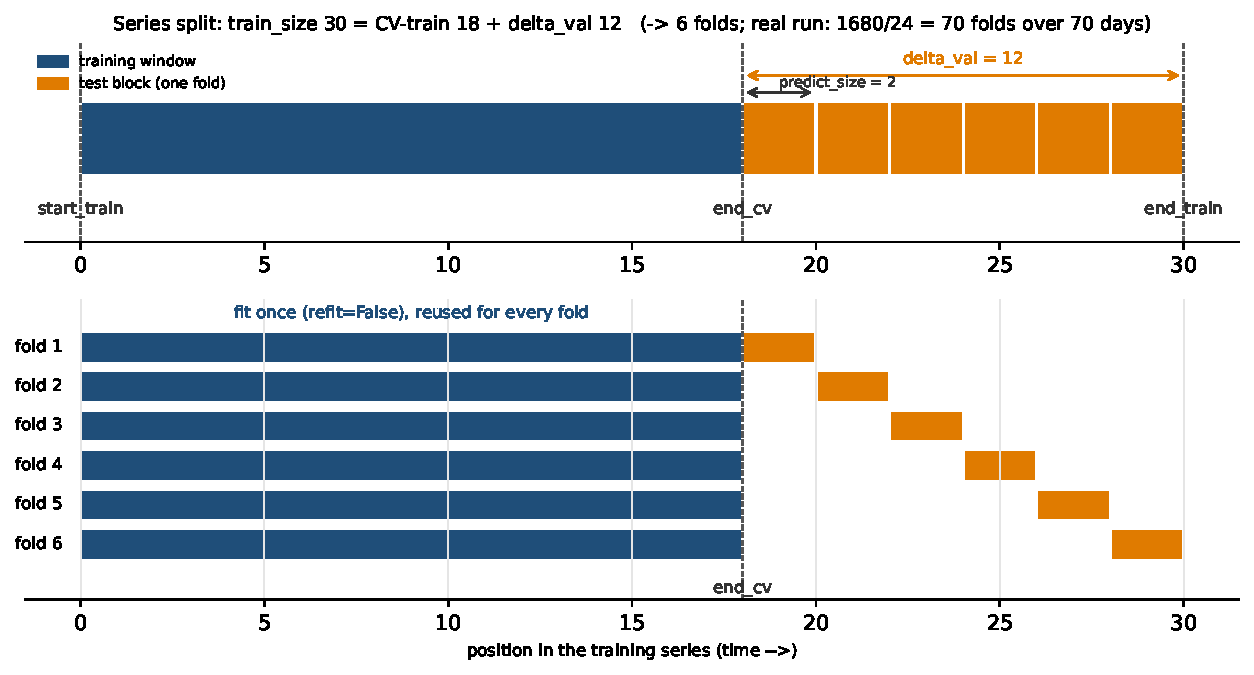
\includegraphics[keepaspectratio]{14_team_4_submission_files/figure-pdf/fig-team4-cv-geometry-output-1.pdf}}

}

\caption{\label{fig-team4-cv-geometry}Cross-validation geometry behind
\texttt{DELTA\_VAL}, drawn with the toy constants
\texttt{predict\_size=2,\ refit\_size=2,\ number\_folds=3,\ train\_size=30}
(so \texttt{delta\_val=12} and 6 folds). Top: the series splits into a
fixed training window \texttt{{[}start\_train,\ end\_cv{]}} (blue) and
the held-out validation span \texttt{delta\_val} (orange), tiled by
non-overlapping \texttt{predict\_size}-wide folds. Bottom: the
rolling-origin back-test --- the model is fit once and reused, the test
block sliding forward one stride per fold. The real run uses the same
picture with 70 daily (\texttt{cv\_block\_size=24}) folds over the
70-day span, independent of the live \texttt{predict\_size}.}

\end{figure}%

\subsubsection{The real configuration}\label{the-real-configuration}

Substituting the chapter's constants reproduces the numbers quoted at
Section~\ref{sec-team4-config}:

\begin{itemize}
\tightlist
\item
  validation span: \texttt{delta\_val\ =\ 24\ ×\ 7\ ×\ 10\ =\ 1680} h =
  70 days, held out as \texttt{(end\_cv,\ end\_train{]}} with
  \texttt{end\_cv\ =\ end\_train\ −\ 70\ days};
\item
  CV training window: \texttt{26280\ −\ 1680\ =\ 24600} h ≈ 2.81 years,
  the fixed block the forecaster is fit on once;
\item
  folds: \texttt{1680\ /\ cv\_block\_size\ =\ 1680\ /\ 24\ =\ 70}
  non-overlapping daily blocks tiling the 70-day span --- the same count
  for every render, because \texttt{cv\_block\_size} is fixed at 24 and
  does not track the live \texttt{predict\_size};
\item
  scored hours: \texttt{70\ ×\ 24\ =\ 1680\ =\ delta\_val}, pooled into
  the single MAE SpotOptim drives down.
\end{itemize}

\subsubsection{How SpotOptim consumes
it}\label{how-spotoptim-consumes-it}

This geometry is the fixed yardstick of the search. Each SpotOptim trial
proposes one hyperparameter candidate --- including a lag set, the
warm-started \texttt{key\_lags} among them
(Section~\ref{sec-team4-config}) --- builds the forecaster, runs the
70-fold rolling back-test above, and returns its pooled MAE. The
surrogate optimiser then picks the next candidate to try, always against
the \emph{same} 1680-hour validation window tiled the \emph{same} way
every render, so trials are directly comparable. Exercise 3 inspects
which lag configuration ultimately won.

\begin{tcolorbox}[enhanced jigsaw, arc=.35mm, bottomrule=.15mm, bottomtitle=1mm, breakable, colback=white, colbacktitle=quarto-callout-note-color!10!white, colframe=quarto-callout-note-color-frame, coltitle=black, left=2mm, leftrule=.75mm, opacityback=0, opacitybacktitle=0.6, rightrule=.15mm, title=\textcolor{quarto-callout-note-color}{\faInfo}\hspace{0.5em}{Why \texttt{cv\_block\_size} is a separate knob}, titlerule=0mm, toprule=.15mm, toptitle=1mm]

The config carries two horizons that are easy to confuse.
\texttt{predict\_size\ =\ LIVE\_N\_STEPS} is the \emph{live} forecast
horizon --- the recursive bridge to tomorrow 23:00, which floats with
the ENTSO-E feed's freshness at render time (≈ 25--48 h).
\texttt{cv\_block\_size\ =\ 24} is the \emph{cross-validation} block ---
the horizon each fold scores. Setting them apart matters for two
reasons:

\begin{itemize}
\tightlist
\item
  The search minimises the pooled MAE of
  \texttt{cv\_block\_size}-step-ahead forecasts. Fixing that at a
  24-hour day keeps the tuning objective aligned with the leaderboard's
  24-hour metric, instead of a longer, render-dependent horizon.
\item
  Because \texttt{cv\_block\_size} is constant, the validation protocol
  (block width and the \texttt{1680/24\ =\ 70} fold count) is identical
  across renders --- the reproducibility (CR-2) the frozen chapters
  enjoy, now kept for the live one.
\end{itemize}

Were the two coupled --- \texttt{cv\_block\_size} left unset, so the CV
inherited \texttt{predict\_size\ =\ LIVE\_N\_STEPS} --- the block would
be ≈ 32 h, the fold count \texttt{⌈1680/32⌉\ =\ 53}, and both would
drift between renders. That coupling is exactly what the
\texttt{cv\_block\_size} field (added in \texttt{spotforecast2-safe})
removes; Exercise 4 probes how much the choice of block actually moves
the tuned model.

\end{tcolorbox}

\subsection{Step 1 --- Endogenous data: prepare and
profile}\label{sec-team4-prepare}

\texttt{prepare\_data()} loads the ENTSO-E DE \texttt{Actual\ Load}
series and aggregates the 15-minute actuals onto the hourly grid the
forecaster expects (the hourly mean of each hour's four quarter-hour
values). We profile it before any curation so later steps have a
baseline to compare against.

\protect\phantomsection\label{team4-prepare}
\begin{Shaded}
\begin{Highlighting}[]
\NormalTok{team4\_mt }\OperatorTok{=}\NormalTok{ MultiTask(team4\_config, task}\OperatorTok{=}\StringTok{"spotoptim"}\NormalTok{)}
\NormalTok{team4\_mt.prepare\_data()}

\NormalTok{endo }\OperatorTok{=}\NormalTok{ team4\_mt.df\_pipeline}
\BuiltInTok{print}\NormalTok{(}\SpecialStringTok{f"df\_pipeline shape: }\SpecialCharTok{\{}\NormalTok{endo}\SpecialCharTok{.}\NormalTok{shape}\SpecialCharTok{\}}\SpecialStringTok{"}\NormalTok{)}
\BuiltInTok{print}\NormalTok{(}\SpecialStringTok{f"index range      : }\SpecialCharTok{\{}\NormalTok{endo}\SpecialCharTok{.}\NormalTok{index}\SpecialCharTok{.}\BuiltInTok{min}\NormalTok{()}\SpecialCharTok{\}}\SpecialStringTok{ → }\SpecialCharTok{\{}\NormalTok{endo}\SpecialCharTok{.}\NormalTok{index}\SpecialCharTok{.}\BuiltInTok{max}\NormalTok{()}\SpecialCharTok{\}}\SpecialStringTok{"}\NormalTok{)}
\BuiltInTok{print}\NormalTok{(}\SpecialStringTok{f"cadence          : }\SpecialCharTok{\{}\NormalTok{endo}\SpecialCharTok{.}\NormalTok{index}\SpecialCharTok{.}\NormalTok{to\_series()}\SpecialCharTok{.}\NormalTok{diff()}\SpecialCharTok{.}\NormalTok{dropna()}\SpecialCharTok{.}\NormalTok{mode()}\SpecialCharTok{.}\NormalTok{iloc[}\DecValTok{0}\NormalTok{]}\SpecialCharTok{\}}\SpecialStringTok{  (hourly mean of the 15{-}min actuals)"}\NormalTok{)}
\BuiltInTok{print}\NormalTok{(endo[}\StringTok{"Actual Load"}\NormalTok{].describe())}
\end{Highlighting}
\end{Shaded}

\begin{verbatim}
INFO:spotforecast2.multitask.base.MultiTask:Pipeline data shape after preparation: (38710, 2)
\end{verbatim}

\begin{verbatim}
df_pipeline shape: (38710, 2)
index range      : 2022-01-01 00:00:00+00:00 → 2026-06-01 21:00:00+00:00
cadence          : 0 days 01:00:00  (hourly mean of the 15-min actuals)
count    38683.000000
mean     53579.879057
std       9355.244530
min      30902.685000
25%      45900.622500
50%      53618.930000
75%      60567.817375
max      78680.352500
Name: Actual Load, dtype: float64
\end{verbatim}

\begin{Shaded}
\begin{Highlighting}[]
\ImportTok{from}\NormalTok{ spotforecast2.plots.time\_series\_visualization }\ImportTok{import}\NormalTok{ visualize\_ts\_plotly}

\NormalTok{visualize\_ts\_plotly(}
\NormalTok{    \{}\StringTok{"Actual Load"}\NormalTok{: team4\_mt.df\_pipeline[[}\StringTok{"Actual Load"}\NormalTok{]]\},}
\NormalTok{    columns}\OperatorTok{=}\NormalTok{[}\StringTok{"Actual Load"}\NormalTok{],}
\NormalTok{)}
\end{Highlighting}
\end{Shaded}

\begin{figure}

\centering{

\begin{verbatim}
Unable to display output for mime type(s): text/html
\end{verbatim}

}

\caption{\label{fig-team4-endogenous}Endogenous target after
\texttt{prepare\_data()} --- the hourly ENTSO-E DE \texttt{Actual\ Load}
series the advanced LGBM forecaster is tuned on, before outlier curation
or imputation.}

\end{figure}%

Figure~\ref{fig-team4-endogenous-last-week} zooms in on the last week of
the endogenous target, which is the most recent data the model trains on
and the closest to the forecast bridge. It is a sanity check that this
window contains no unexpected gaps or anomalies before we hand it to the
outlier detection step in Section~\ref{sec-team4-outliers}.

\begin{Shaded}
\begin{Highlighting}[]
\ImportTok{from}\NormalTok{ spotforecast2.plots.time\_series\_visualization }\ImportTok{import}\NormalTok{ visualize\_ts\_plotly}

\NormalTok{last\_week }\OperatorTok{=}\NormalTok{ team4\_mt.df\_pipeline.loc[}
\NormalTok{    team4\_mt.df\_pipeline.index.}\BuiltInTok{max}\NormalTok{() }\OperatorTok{{-}}\NormalTok{ pd.Timedelta(days}\OperatorTok{=}\DecValTok{7}\NormalTok{):, [}\StringTok{"Actual Load"}\NormalTok{]}
\NormalTok{]}
\NormalTok{visualize\_ts\_plotly(}
\NormalTok{    \{}\StringTok{"Actual Load"}\NormalTok{: last\_week\},}
\NormalTok{    columns}\OperatorTok{=}\NormalTok{[}\StringTok{"Actual Load"}\NormalTok{],}
\NormalTok{)}
\end{Highlighting}
\end{Shaded}

\begin{figure}

\centering{

\begin{verbatim}
Unable to display output for mime type(s): text/html
\end{verbatim}

}

\caption{\label{fig-team4-endogenous-last-week}Last week data of the
endogenous target after \texttt{prepare\_data()}}

\end{figure}%

\subsection{Step 2 --- Outlier detection and
curation}\label{sec-team4-outliers}

Curation needs a bound. A fixed pair such as \texttt{±1e9} MW flags
nothing, so it removes nothing; a tight pair risks deleting genuine
demand --- the January cold-snap peaks and the holiday troughs are real
records the model must see. We want the opposite of both: bounds wide
enough to keep every plausible value, narrow enough to excise the
physically impossible ones (a reported 0 MW national load, a sensor
spike to ten times the peak).

We therefore derive the bounds from the load history itself, using a
robust rule that the anomalies cannot distort. Let \(m\) be the median
of the series and \(\mathrm{IQR}\) its inter-quartile range (the 75th
minus the 25th percentile). Median and IQR are \emph{robust}: a handful
of absurd records barely moves them, so the band they define is not
inflated by the very points we mean to catch. The bounds are

\[
\text{lower} = \max(0,\; m - K\cdot\mathrm{IQR}), \qquad
\text{upper} = m + K\cdot\mathrm{IQR},
\]

with \(K = 5\) --- a deliberately \emph{relaxed} width. (For reference,
Tukey's ``far out'' fence uses \(K = 3\); ours is wider still.) For
German load this places the band at roughly \([0,\,130]\) GW, so only
records outside any plausible national demand are flagged. The lower
bound is floored at 0 MW because load cannot be negative.
\texttt{OUTLIER\_IQR\_K} is exposed as a constant: lower it to curate
more aggressively, raise it to curate only the most extreme records.

We compute the bounds from the prepared history and assign them to
\texttt{team4\_mt.config.bounds} \emph{before} detection runs.

\protect\phantomsection\label{team4-outlier-bounds}
\begin{Shaded}
\begin{Highlighting}[]
\NormalTok{OUTLIER\_IQR\_K }\OperatorTok{=} \DecValTok{5}

\NormalTok{s }\OperatorTok{=}\NormalTok{ team4\_mt.df\_pipeline[}\StringTok{"Actual Load"}\NormalTok{].dropna()}
\NormalTok{med }\OperatorTok{=}\NormalTok{ s.median()}
\NormalTok{iqr }\OperatorTok{=}\NormalTok{ s.quantile(}\FloatTok{0.75}\NormalTok{) }\OperatorTok{{-}}\NormalTok{ s.quantile(}\FloatTok{0.25}\NormalTok{)}
\NormalTok{low }\OperatorTok{=} \BuiltInTok{max}\NormalTok{(}\FloatTok{0.0}\NormalTok{, med }\OperatorTok{{-}}\NormalTok{ OUTLIER\_IQR\_K }\OperatorTok{*}\NormalTok{ iqr)}
\NormalTok{high }\OperatorTok{=}\NormalTok{ med }\OperatorTok{+}\NormalTok{ OUTLIER\_IQR\_K }\OperatorTok{*}\NormalTok{ iqr}
\NormalTok{team4\_mt.config.bounds }\OperatorTok{=}\NormalTok{ [(low, high)]}

\NormalTok{n\_outside }\OperatorTok{=} \BuiltInTok{int}\NormalTok{(((s }\OperatorTok{\textless{}}\NormalTok{ low) }\OperatorTok{|}\NormalTok{ (s }\OperatorTok{\textgreater{}}\NormalTok{ high)).}\BuiltInTok{sum}\NormalTok{())}
\BuiltInTok{print}\NormalTok{(}\SpecialStringTok{f"median             : }\SpecialCharTok{\{}\NormalTok{med}\SpecialCharTok{:,.0f\}}\SpecialStringTok{ MW"}\NormalTok{)}
\BuiltInTok{print}\NormalTok{(}\SpecialStringTok{f"IQR                : }\SpecialCharTok{\{}\NormalTok{iqr}\SpecialCharTok{:,.0f\}}\SpecialStringTok{ MW"}\NormalTok{)}
\BuiltInTok{print}\NormalTok{(}\SpecialStringTok{f"derived bounds (K=}\SpecialCharTok{\{}\NormalTok{OUTLIER\_IQR\_K}\SpecialCharTok{\}}\SpecialStringTok{): [}\SpecialCharTok{\{}\NormalTok{low}\SpecialCharTok{:,.0f\}}\SpecialStringTok{, }\SpecialCharTok{\{}\NormalTok{high}\SpecialCharTok{:,.0f\}}\SpecialStringTok{] MW"}\NormalTok{)}
\BuiltInTok{print}\NormalTok{(}\SpecialStringTok{f"history points out : }\SpecialCharTok{\{}\NormalTok{n\_outside}\SpecialCharTok{\}}\SpecialStringTok{ of }\SpecialCharTok{\{}\BuiltInTok{len}\NormalTok{(s)}\SpecialCharTok{\}}\SpecialStringTok{"}\NormalTok{)}
\end{Highlighting}
\end{Shaded}

\begin{verbatim}
median             : 53,619 MW
IQR                : 14,667 MW
derived bounds (K=5): [0, 126,955] MW
history points out : 0 of 38683
\end{verbatim}

\texttt{detect\_outliers()} snapshots the pre-curation series into
\texttt{df\_pipeline\_original}, then replaces every value outside these
bounds with NaN in \texttt{df\_pipeline} via
\texttt{manual\_outlier\_removal} (the values are \emph{replaced}, not
clipped to the bound). The second branch of \texttt{detect\_outliers()}
runs an IsolationForest pass (\texttt{get\_outliers},
\texttt{contamination=0.01}), but that call only \emph{reports}
candidate anomalies to the log --- it does not alter the series. The
hard bounds are therefore the sole mechanism that marks NaN. Removing
implausible values here is a direct Art. 10 data governance obligation:
the model must not learn from corrupted records.

What happens to a flagged record next is the substance of curation, and
it is not deletion. The recursive LightGBM forecaster reads
autoregressive lags off a \emph{contiguous} hourly index; dropping rows
outright would misalign every downstream lag. Instead, Step 3
(Section~\ref{sec-team4-impute}) imputes the NaN with the default
\texttt{weighted} strategy: it forward/back-fills the gap so the index
stays gap-free, \emph{and} it builds a sample-weight function that
assigns weight 0 to each imputed timestamp and the surrounding
\texttt{imputation\_window\_size} h (here 24 h). That weight function is
threaded into the forecaster
(\texttt{ForecasterRecursive(weight\_func=…)}), so during \texttt{fit}
the curated rows contribute nothing to the training loss and nothing to
the validation score. A flagged record is thus replaced by NaN, filled
only to preserve lag continuity, and \emph{excluded from training and
validation} by zero weight --- the intended Art. 10 outcome, reached
without breaking the recursive feature construction.

\texttt{imputation\_window\_size} is a dedicated knob: it sets the
gap-penalty width \emph{independently} of \texttt{window\_size} (default
72 h), which still controls the LightGBM rolling-mean feature window.
During tuning SpotOptim evaluates many short cross-validation folds, and
a fold lying entirely inside a penalty zone has every row at weight 0;
the forecaster then logs \emph{``all sample weights for the requested
index are zero \ldots{} using uniform weighting''} and falls back to
uniform weights for that fold. This is benign --- it is the safe
degenerate case, not an error --- but a narrower
\texttt{imputation\_window\_size} makes it rarer without widening the
rolling-feature window.

\protect\phantomsection\label{team4-detect-outliers}
\begin{Shaded}
\begin{Highlighting}[]
\NormalTok{team4\_mt.detect\_outliers()}

\NormalTok{n\_removed }\OperatorTok{=} \BuiltInTok{int}\NormalTok{(}
\NormalTok{    (team4\_mt.df\_pipeline[}\StringTok{"Actual Load"}\NormalTok{].isna()}
     \OperatorTok{\&}\NormalTok{ team4\_mt.df\_pipeline\_original[}\StringTok{"Actual Load"}\NormalTok{].notna()).}\BuiltInTok{sum}\NormalTok{()}
\NormalTok{)}
\NormalTok{nan\_to\_impute }\OperatorTok{=} \BuiltInTok{int}\NormalTok{(team4\_mt.df\_pipeline[}\StringTok{"Actual Load"}\NormalTok{].isna().}\BuiltInTok{sum}\NormalTok{())}
\NormalTok{imputed\_idx }\OperatorTok{=}\NormalTok{ team4\_mt.df\_pipeline.index[team4\_mt.df\_pipeline[}\StringTok{"Actual Load"}\NormalTok{].isna()]}
\CommentTok{\# Split genuine interior gaps from the unpublished trailing tail (@sec{-}team4{-}availability):}
\CommentTok{\# anything at or before end\_train (LAST\_FULL\_HOUR) is a real gap; anything after it is}
\CommentTok{\# simply the recent tail ENTSO{-}E has not published yet, which end\_train excludes from y\_train.}
\NormalTok{interior\_idx }\OperatorTok{=}\NormalTok{ imputed\_idx[imputed\_idx }\OperatorTok{\textless{}=}\NormalTok{ LAST\_FULL\_HOUR]}
\NormalTok{tail\_idx }\OperatorTok{=}\NormalTok{ imputed\_idx[imputed\_idx }\OperatorTok{\textgreater{}}\NormalTok{ LAST\_FULL\_HOUR]}
\NormalTok{contamination }\OperatorTok{=} \BuiltInTok{getattr}\NormalTok{(team4\_mt.config, }\StringTok{"contamination"}\NormalTok{, }\VariableTok{None}\NormalTok{)}

\BuiltInTok{print}\NormalTok{(}\SpecialStringTok{f"outliers removed   : }\SpecialCharTok{\{}\NormalTok{n\_removed}\SpecialCharTok{\}}\SpecialStringTok{"}\NormalTok{)}
\BuiltInTok{print}\NormalTok{(}\SpecialStringTok{f"NaN to impute next : }\SpecialCharTok{\{}\NormalTok{nan\_to\_impute}\SpecialCharTok{\}}\SpecialStringTok{"}\NormalTok{)}
\BuiltInTok{print}\NormalTok{(}\SpecialStringTok{f"  interior gaps    : }\SpecialCharTok{\{}\BuiltInTok{len}\NormalTok{(interior\_idx)}\SpecialCharTok{\}}\SpecialStringTok{  (real gaps in observed range)"}\NormalTok{)}
\BuiltInTok{print}\NormalTok{(}\SpecialStringTok{f"  trailing tail    : }\SpecialCharTok{\{}\BuiltInTok{len}\NormalTok{(tail\_idx)}\SpecialCharTok{\}}\SpecialStringTok{  (unpublished, after end\_train)"}\NormalTok{)}
\BuiltInTok{print}\NormalTok{(}\SpecialStringTok{f"contamination      : }\SpecialCharTok{\{}\NormalTok{contamination}\SpecialCharTok{\}}\SpecialStringTok{"}\NormalTok{)}
\end{Highlighting}
\end{Shaded}

\begin{verbatim}
INFO:spotforecast2.multitask.base.MultiTask:Forecasted Load: 366 outliers automatically detected
INFO:spotforecast2.multitask.base.MultiTask:Actual Load: 388 outliers automatically detected
INFO:spotforecast2.multitask.base.MultiTask:Outlier detection complete.
\end{verbatim}

\begin{verbatim}
outliers removed   : 0
NaN to impute next : 27
  interior gaps    : 0  (real gaps in observed range)
  trailing tail    : 27  (unpublished, after end_train)
contamination      : 0.01
\end{verbatim}

\begin{Shaded}
\begin{Highlighting}[]
\ImportTok{from}\NormalTok{ spotforecast2.plots.plotter }\ImportTok{import}\NormalTok{ plot\_with\_outliers}

\NormalTok{plot\_with\_outliers(team4\_mt.df\_pipeline, team4\_mt.df\_pipeline\_original, team4\_mt.config)}
\end{Highlighting}
\end{Shaded}

\begin{figure}

\centering{

\begin{verbatim}
Unable to display output for mime type(s): text/html
\end{verbatim}

}

\caption{\label{fig-team4-outliers}Outlier curation as performed by the
pipeline: the pre-curation series (\texttt{df\_pipeline\_original})
overlaid with the curated series (\texttt{df\_pipeline}), with removed
points marked.}

\end{figure}%

\subsection{Step 3 --- Missing-data imputation}\label{sec-team4-impute}

\texttt{impute()} fills the gaps left by curation (and any pre-existing
gaps) so the recursive forecaster sees a gap-free series. Under Art. 10
every filled value is a modelling assumption, so we verify the count
goes to zero rather than trusting the call silently.

Of the \texttt{nan\_to\_impute} missing values, only
\texttt{interior\_idx} are genuine gaps inside the observed range; the
rest (\texttt{tail\_idx}) is the unpublished trailing tail described in
Section~\ref{sec-team4-availability} --- the forecast-bridge hours after
\texttt{end\_train} that ENTSO-E has not published yet. Filling the tail
is harmless: \texttt{end\_train} excludes it from the training target
\texttt{y\_train}, so the model never fits the imputed tail values. The
visualization below therefore zooms in only on the genuine interior
gaps; on a typical render there are none, and the fallback view of the
most recent hours is shown instead.

\protect\phantomsection\label{team4-impute}
\begin{Shaded}
\begin{Highlighting}[]
\NormalTok{team4\_mt.impute()}

\NormalTok{nan\_after }\OperatorTok{=} \BuiltInTok{int}\NormalTok{(team4\_mt.df\_pipeline[}\StringTok{"Actual Load"}\NormalTok{].isna().}\BuiltInTok{sum}\NormalTok{())}
\BuiltInTok{print}\NormalTok{(}\SpecialStringTok{f"NaN before impute: }\SpecialCharTok{\{}\NormalTok{nan\_to\_impute}\SpecialCharTok{\}}\SpecialStringTok{"}\NormalTok{)}
\BuiltInTok{print}\NormalTok{(}\SpecialStringTok{f"NaN after impute : }\SpecialCharTok{\{}\NormalTok{nan\_after}\SpecialCharTok{\}}\SpecialStringTok{  (must be 0)"}\NormalTok{)}
\end{Highlighting}
\end{Shaded}

\begin{verbatim}
INFO:spotforecast2.multitask.base.MultiTask:apply_imputation: NaN cells before imputation: 27 (method='weighted', shape=(38710, 2))
INFO:spotforecast2.multitask.base.MultiTask:Applying weighted imputation (n2n style)...
INFO:spotforecast2.multitask.base.MultiTask:Weight function created with 38710 entries.
INFO:spotforecast2.multitask.base.MultiTask:apply_imputation: NaN cells after imputation: 0
INFO:spotforecast2.multitask.base.MultiTask:Imputation complete (method=weighted).
\end{verbatim}

\begin{verbatim}
NaN before impute: 27
NaN after impute : 0  (must be 0)
\end{verbatim}

\begin{Shaded}
\begin{Highlighting}[]
\BuiltInTok{print}\NormalTok{(}\SpecialStringTok{f"interior gaps to plot: }\SpecialCharTok{\{}\BuiltInTok{len}\NormalTok{(interior\_idx)}\SpecialCharTok{\}}\SpecialStringTok{  "}
      \SpecialStringTok{f"(trailing tail of }\SpecialCharTok{\{}\BuiltInTok{len}\NormalTok{(tail\_idx)}\SpecialCharTok{\}}\SpecialStringTok{ unpublished hours not shown)"}\NormalTok{)}
\ControlFlowTok{if} \BuiltInTok{len}\NormalTok{(interior\_idx) }\OperatorTok{\textgreater{}} \DecValTok{0}\NormalTok{:}
    \CommentTok{\# Reconstruct the pre{-}imputation (gapped) series by re{-}inserting NaN at the}
    \CommentTok{\# interior gap positions; the imputed series is df\_pipeline after impute().}
\NormalTok{    gapped }\OperatorTok{=}\NormalTok{ team4\_mt.df\_pipeline[[}\StringTok{"Actual Load"}\NormalTok{]].copy()}
\NormalTok{    gapped.loc[gapped.index.isin(interior\_idx), }\StringTok{"Actual Load"}\NormalTok{] }\OperatorTok{=} \BuiltInTok{float}\NormalTok{(}\StringTok{"nan"}\NormalTok{)}
\NormalTok{    imputed }\OperatorTok{=}\NormalTok{ team4\_mt.df\_pipeline[[}\StringTok{"Actual Load"}\NormalTok{]]}

    \BuiltInTok{print}\NormalTok{(}\SpecialStringTok{f"plotting }\SpecialCharTok{\{}\BuiltInTok{len}\NormalTok{(interior\_idx)}\SpecialCharTok{\}}\SpecialStringTok{ interior gaps (±12 h window each)"}\NormalTok{)}
    \ControlFlowTok{for}\NormalTok{ i, t }\KeywordTok{in} \BuiltInTok{enumerate}\NormalTok{(interior\_idx, start}\OperatorTok{=}\DecValTok{1}\NormalTok{):}
\NormalTok{        w }\OperatorTok{=} \BuiltInTok{slice}\NormalTok{(t }\OperatorTok{{-}}\NormalTok{ pd.Timedelta(hours}\OperatorTok{=}\DecValTok{12}\NormalTok{), t }\OperatorTok{+}\NormalTok{ pd.Timedelta(hours}\OperatorTok{=}\DecValTok{12}\NormalTok{))}
\NormalTok{        visualize\_ts\_plotly(}
\NormalTok{            \{}
                \StringTok{"before (gaps)"}\NormalTok{:   gapped.loc[w],}
                \StringTok{"after (imputed)"}\NormalTok{: imputed.loc[w],}
\NormalTok{            \},}
\NormalTok{            columns}\OperatorTok{=}\NormalTok{[}\StringTok{"Actual Load"}\NormalTok{],}
\NormalTok{            title\_suffix}\OperatorTok{=}\SpecialStringTok{f"— gap }\SpecialCharTok{\{}\NormalTok{i}\SpecialCharTok{\}}\SpecialStringTok{/}\SpecialCharTok{\{}\BuiltInTok{len}\NormalTok{(interior\_idx)}\SpecialCharTok{\}}\SpecialStringTok{ @ }\SpecialCharTok{\{}\NormalTok{t}\SpecialCharTok{:}\OperatorTok{\%}\NormalTok{Y}\OperatorTok{{-}\%}\NormalTok{m}\OperatorTok{{-}\%}\NormalTok{d }\OperatorTok{\%}\NormalTok{H}\SpecialCharTok{:}\OperatorTok{\%}\NormalTok{M}\SpecialCharTok{\}}\SpecialStringTok{"}\NormalTok{,}
\NormalTok{        )}
\ControlFlowTok{else}\NormalTok{:}
    \BuiltInTok{print}\NormalTok{(}\StringTok{"no interior gaps; showing the last 72 hours of the imputed series"}\NormalTok{)}
\NormalTok{    tail }\OperatorTok{=}\NormalTok{ team4\_mt.df\_pipeline[[}\StringTok{"Actual Load"}\NormalTok{]].tail(}\DecValTok{72}\NormalTok{)}
\NormalTok{    visualize\_ts\_plotly(\{}\StringTok{"after (imputed)"}\NormalTok{: tail\}, columns}\OperatorTok{=}\NormalTok{[}\StringTok{"Actual Load"}\NormalTok{])}
\end{Highlighting}
\end{Shaded}

\begin{verbatim}
interior gaps to plot: 0  (trailing tail of 27 unpublished hours not shown)
no interior gaps; showing the last 72 hours of the imputed series
\end{verbatim}

\begin{figure}

\centering{

\begin{verbatim}
Unable to display output for mime type(s): text/html
\end{verbatim}

}

\caption{\label{fig-team4-imputation}One panel per genuine interior gap:
the curated series with the gap (\texttt{before}) overlaid with the
imputed series (\texttt{after}) on a 24-hour window (±12 h) centred on
each imputed timestamp. The unpublished trailing tail
(Section~\ref{sec-team4-availability}) is excluded. If there are no
interior gaps, the last 72 hours of the imputed series are shown
instead.}

\end{figure}%

\subsection{Step 4 --- Exogenous features: weather, holidays, calendar,
polynomial}\label{sec-team4-exog}

\texttt{build\_exogenous\_features()} encodes every exogenous family
enabled in \texttt{team4\_config} --- weather and its rolling windows,
DE/NW public holidays, the five seasonal radial basis function (RBF) /
cyclical encodings, and (because \texttt{poly\_features\_degree=2}) the
bilinear polynomial interactions, capped to the
\texttt{max\_poly\_features=10} most informative ones by mutual
information. We group the generated columns by family at runtime (the
exact encoded names depend on the configuration) and count each family.

\protect\phantomsection\label{team4-build-exog}
\begin{Shaded}
\begin{Highlighting}[]
\NormalTok{team4\_mt.build\_exogenous\_features()}

\NormalTok{exog\_all }\OperatorTok{=}\NormalTok{ team4\_mt.exogenous\_features}
\CommentTok{\# print the full list of exogenous features for manual inspection, then count by family}
\BuiltInTok{print}\NormalTok{(}\StringTok{"exogenous features:"}\NormalTok{)}
\ControlFlowTok{for}\NormalTok{ col }\KeywordTok{in}\NormalTok{ exog\_all.columns:}
    \BuiltInTok{print}\NormalTok{(}\SpecialStringTok{f"  }\SpecialCharTok{\{}\NormalTok{col}\SpecialCharTok{\}}\SpecialStringTok{"}\NormalTok{)}
    
\BuiltInTok{print}\NormalTok{(}\SpecialStringTok{f"exogenous\_features shape : }\SpecialCharTok{\{}\NormalTok{exog\_all}\SpecialCharTok{.}\NormalTok{shape}\SpecialCharTok{\}}\SpecialStringTok{"}\NormalTok{)}
\BuiltInTok{print}\NormalTok{(}\SpecialStringTok{f"selected for training    : }\SpecialCharTok{\{}\BuiltInTok{len}\NormalTok{(team4\_mt.exog\_feature\_names)}\SpecialCharTok{\}}\SpecialStringTok{ features"}\NormalTok{)}

\KeywordTok{def}\NormalTok{ family\_of(col):}
\NormalTok{    c }\OperatorTok{=}\NormalTok{ col.lower()}
    \ControlFlowTok{if} \StringTok{"holiday"} \KeywordTok{in}\NormalTok{ c:}
        \ControlFlowTok{return} \StringTok{"holiday"}
    \ControlFlowTok{if} \StringTok{"poly"} \KeywordTok{in}\NormalTok{ c:}
        \ControlFlowTok{return} \StringTok{"polynomial"}
    \ControlFlowTok{if} \StringTok{"window"} \KeywordTok{in}\NormalTok{ c:}
        \ControlFlowTok{return} \StringTok{"weather\_window"}
    \ControlFlowTok{if} \BuiltInTok{any}\NormalTok{(k }\KeywordTok{in}\NormalTok{ c }\ControlFlowTok{for}\NormalTok{ k }\KeywordTok{in}\NormalTok{ (}\StringTok{"sin"}\NormalTok{, }\StringTok{"cos"}\NormalTok{, }\StringTok{"rbf"}\NormalTok{)):}
        \ControlFlowTok{return} \StringTok{"cyclical/RBF"}
    \ControlFlowTok{if}\NormalTok{ c.startswith(}\StringTok{"lag\_"}\NormalTok{) }\KeywordTok{or}\NormalTok{ c.startswith(}\StringTok{"lag"}\NormalTok{):}
        \ControlFlowTok{return} \StringTok{"lag"}
    \ControlFlowTok{return} \StringTok{"weather/other"}

\NormalTok{families }\OperatorTok{=}\NormalTok{ \{\}}
\ControlFlowTok{for}\NormalTok{ col }\KeywordTok{in}\NormalTok{ exog\_all.columns:}
\NormalTok{    families.setdefault(family\_of(col), []).append(col)}

\NormalTok{counts }\OperatorTok{=}\NormalTok{ pd.DataFrame(}
    \BuiltInTok{sorted}\NormalTok{(((fam, }\BuiltInTok{len}\NormalTok{(cols)) }\ControlFlowTok{for}\NormalTok{ fam, cols }\KeywordTok{in}\NormalTok{ families.items()),}
\NormalTok{           key}\OperatorTok{=}\KeywordTok{lambda}\NormalTok{ kv: kv[}\DecValTok{1}\NormalTok{], reverse}\OperatorTok{=}\VariableTok{True}\NormalTok{),}
\NormalTok{    columns}\OperatorTok{=}\NormalTok{[}\StringTok{"family"}\NormalTok{, }\StringTok{"count"}\NormalTok{],}
\NormalTok{)}
\BuiltInTok{print}\NormalTok{(counts.to\_string(index}\OperatorTok{=}\VariableTok{False}\NormalTok{))}
\end{Highlighting}
\end{Shaded}

\begin{verbatim}
INFO:spotforecast2.multitask.base.MultiTask:Building exogenous features...
INFO:spotforecast2.multitask.base.MultiTask:  Weather features: (38739, 105)
INFO:spotforecast2.multitask.base.MultiTask:  Calendar features: (38739, 4)
INFO:spotforecast2.multitask.base.MultiTask:  Day/night features: (38739, 4)
INFO:spotforecast2.multitask.base.MultiTask:  Holiday features: (38739, 1)
INFO:spotforecast2.multitask.base.MultiTask:Capped polynomial features: kept 10 of 5995 (dropped 5985).
INFO:spotforecast2.multitask.base.MultiTask:Combined exogenous features shape: (38739, 136)
INFO:spotforecast2.multitask.base.MultiTask:Selected 127 exogenous features for training.
INFO:spotforecast2.multitask.base.MultiTask:Merged data shape: (38710, 128)
INFO:spotforecast2.multitask.base.MultiTask:Exogenous prediction covariates shape: (29, 136)
\end{verbatim}

\begin{verbatim}
exogenous features:
  month
  week
  day_of_week
  hour
  sunrise_hour
  sunset_hour
  daylight_hours
  is_daylight
  temperature_2m
  relative_humidity_2m
  precipitation
  rain
  snowfall
  weather_code
  pressure_msl
  surface_pressure
  cloud_cover
  cloud_cover_low
  cloud_cover_mid
  cloud_cover_high
  wind_speed_10m
  wind_direction_10m
  wind_gusts_10m
  temperature_2m_window_1D_mean
  temperature_2m_window_1D_max
  temperature_2m_window_1D_min
  relative_humidity_2m_window_1D_mean
  relative_humidity_2m_window_1D_max
  relative_humidity_2m_window_1D_min
  precipitation_window_1D_mean
  precipitation_window_1D_max
  precipitation_window_1D_min
  rain_window_1D_mean
  rain_window_1D_max
  rain_window_1D_min
  snowfall_window_1D_mean
  snowfall_window_1D_max
  snowfall_window_1D_min
  weather_code_window_1D_mean
  weather_code_window_1D_max
  weather_code_window_1D_min
  pressure_msl_window_1D_mean
  pressure_msl_window_1D_max
  pressure_msl_window_1D_min
  surface_pressure_window_1D_mean
  surface_pressure_window_1D_max
  surface_pressure_window_1D_min
  cloud_cover_window_1D_mean
  cloud_cover_window_1D_max
  cloud_cover_window_1D_min
  cloud_cover_low_window_1D_mean
  cloud_cover_low_window_1D_max
  cloud_cover_low_window_1D_min
  cloud_cover_mid_window_1D_mean
  cloud_cover_mid_window_1D_max
  cloud_cover_mid_window_1D_min
  cloud_cover_high_window_1D_mean
  cloud_cover_high_window_1D_max
  cloud_cover_high_window_1D_min
  wind_speed_10m_window_1D_mean
  wind_speed_10m_window_1D_max
  wind_speed_10m_window_1D_min
  wind_direction_10m_window_1D_mean
  wind_direction_10m_window_1D_max
  wind_direction_10m_window_1D_min
  wind_gusts_10m_window_1D_mean
  wind_gusts_10m_window_1D_max
  wind_gusts_10m_window_1D_min
  temperature_2m_window_7D_mean
  temperature_2m_window_7D_max
  temperature_2m_window_7D_min
  relative_humidity_2m_window_7D_mean
  relative_humidity_2m_window_7D_max
  relative_humidity_2m_window_7D_min
  precipitation_window_7D_mean
  precipitation_window_7D_max
  precipitation_window_7D_min
  rain_window_7D_mean
  rain_window_7D_max
  rain_window_7D_min
  snowfall_window_7D_mean
  snowfall_window_7D_max
  snowfall_window_7D_min
  weather_code_window_7D_mean
  weather_code_window_7D_max
  weather_code_window_7D_min
  pressure_msl_window_7D_mean
  pressure_msl_window_7D_max
  pressure_msl_window_7D_min
  surface_pressure_window_7D_mean
  surface_pressure_window_7D_max
  surface_pressure_window_7D_min
  cloud_cover_window_7D_mean
  cloud_cover_window_7D_max
  cloud_cover_window_7D_min
  cloud_cover_low_window_7D_mean
  cloud_cover_low_window_7D_max
  cloud_cover_low_window_7D_min
  cloud_cover_mid_window_7D_mean
  cloud_cover_mid_window_7D_max
  cloud_cover_mid_window_7D_min
  cloud_cover_high_window_7D_mean
  cloud_cover_high_window_7D_max
  cloud_cover_high_window_7D_min
  wind_speed_10m_window_7D_mean
  wind_speed_10m_window_7D_max
  wind_speed_10m_window_7D_min
  wind_direction_10m_window_7D_mean
  wind_direction_10m_window_7D_max
  wind_direction_10m_window_7D_min
  wind_gusts_10m_window_7D_mean
  wind_gusts_10m_window_7D_max
  wind_gusts_10m_window_7D_min
  is_holiday
  month_sin
  month_cos
  week_sin
  week_cos
  day_of_week_sin
  day_of_week_cos
  hour_sin
  hour_cos
  sunrise_hour_sin
  sunrise_hour_cos
  sunset_hour_sin
  sunset_hour_cos
  poly_hour_cos__temperature_2m_window_1D_mean
  poly_hour_cos__temperature_2m_window_1D_max
  poly_hour_cos__temperature_2m_window_7D_mean
  poly_hour_cos__temperature_2m_window_7D_max
  poly_hour_cos__weather_code_window_7D_max
  poly_hour_cos__pressure_msl_window_7D_max
  poly_hour_cos__pressure_msl_window_7D_min
  poly_hour_cos__surface_pressure_window_7D_max
  poly_hour_cos__surface_pressure_window_7D_min
  poly_hour_cos__temperature_2m
exogenous_features shape : (38739, 136)
selected for training    : 127 features
        family  count
weather_window     90
 weather/other     23
  cyclical/RBF     12
    polynomial     10
       holiday      1
\end{verbatim}

\subsection{Processing of the Weather Data}\label{sec-team4-weather}

\texttt{build\_exogenous\_features()} pulls weather from the Open-Meteo
API through \texttt{get\_weather\_features()} (in
\texttt{spotforecast2\_safe.weather.features}). It fetches hourly
\texttt{temperature\_2m} --- the dominant load driver below
\textasciitilde5 °C and above \textasciitilde15 °C --- plus fourteen
other variables for the Dortmund default location (51.5136 °N, 7.4653
°E; the \texttt{state="NW"} setting drives the \emph{holiday} calendar,
not the weather coordinates), caches them as a parquet file, and derives
the rolling 1-day and 7-day mean/max/min window features enabled by
\texttt{include\_weather\_windows=True}. The result is stored as
\texttt{team4\_mt.weather\_aligned} and plotted against load below.

The interesting part is the recent edge of the series, because
Open-Meteo serves two endpoints with a coverage seam. The \emph{archive}
endpoint carries quality-checked history but lags about five days; the
\emph{forecast} endpoint carries today and the days ahead, and --- via
its \texttt{past\_days} parameter --- a configurable number of recent
days backwards. \texttt{\_fetch\_hybrid()} stitches them together: it
takes the archive up to \texttt{now\ -\ 5\ days} and the forecast with
enough \texttt{past\_days} to bridge that five-day lag plus enough
\texttt{forecast\_days} to reach the prediction horizon. This is the
weather analogue of the ENTSO-E publication lag in
Section~\ref{sec-team4-availability}: the most recent days are not yet
in the historical record.

A worked example makes the seam concrete. The cell below recomputes, for
this render, the two numbers that close it.

\protect\phantomsection\label{team4-weather-window}
\begin{Shaded}
\begin{Highlighting}[]
\NormalTok{archive\_cutoff }\OperatorTok{=}\NormalTok{ NOW\_UTC }\OperatorTok{{-}}\NormalTok{ pd.Timedelta(days}\OperatorTok{=}\DecValTok{5}\NormalTok{)}
\NormalTok{past\_days }\OperatorTok{=}\NormalTok{ (NOW\_UTC.normalize() }\OperatorTok{{-}}\NormalTok{ archive\_cutoff.normalize()).days }\OperatorTok{+} \DecValTok{1}

\BuiltInTok{print}\NormalTok{(}\SpecialStringTok{f"now (render)       : }\SpecialCharTok{\{}\NormalTok{NOW\_UTC}\SpecialCharTok{\}}\SpecialStringTok{"}\NormalTok{)}
\BuiltInTok{print}\NormalTok{(}\SpecialStringTok{f"archive reaches    : }\SpecialCharTok{\{}\NormalTok{archive\_cutoff}\SpecialCharTok{\}}\SpecialStringTok{   (Open{-}Meteo archive lags \textasciitilde{}5 days)"}\NormalTok{)}
\BuiltInTok{print}\NormalTok{(}\SpecialStringTok{f"forecast past\_days : }\SpecialCharTok{\{}\NormalTok{past\_days}\SpecialCharTok{\}}\SpecialStringTok{         (bridges the 5{-}day archive lag)"}\NormalTok{)}
\BuiltInTok{print}\NormalTok{(}\SpecialStringTok{f"ffill tolerance    : 24 h                (longer gaps are refused, not filled)"}\NormalTok{)}
\end{Highlighting}
\end{Shaded}

\begin{verbatim}
now (render)       : 2026-05-31 19:37:53.771067+00:00
archive reaches    : 2026-05-26 19:37:53.771067+00:00   (Open-Meteo archive lags ~5 days)
forecast past_days : 6         (bridges the 5-day archive lag)
ffill tolerance    : 24 h                (longer gaps are refused, not filled)
\end{verbatim}

For a render at \texttt{now\ =\ 2026-05-31\ 14:00\ UTC} the archive
reaches only \texttt{2026-05-26}, and the forecast is requested with
\texttt{past\_days\ =\ 6}, so it returns from \texttt{2026-05-25\ 00:00}
onward (with \texttt{forecast\_days} reaching the next day's horizon).
The archive window \texttt{{[}…,\ 2026-05-26{]}} and the forecast window
\texttt{{[}2026-05-25,\ 2026-06-03{]}} overlap and jointly cover the
requested range with no hole. Were \texttt{past\_days} omitted, the
forecast would start at \texttt{2026-05-31\ 00:00} and the five days
\texttt{2026-05-26}\ldots{}\texttt{2026-05-30} (≈120 h) would be fetched
by neither endpoint.

That seam is exactly where missing weather data must be handled
correctly. After fetching, the frame is reindexed onto a regular hourly
grid spanning \texttt{{[}data\_start,\ cov\_end{]}}, where
\texttt{cov\_end} is \texttt{end\_train} plus the \texttt{predict\_size}
horizon. Two fail-loud tiers then govern any remaining gap, both active
because the safe default \texttt{fill\_missing=False} applies:

\begin{itemize}
\tightlist
\item
  The fetch layer (\texttt{\_finalize\_df}) rejects any interior
  \texttt{NaN} or absent hour and reports the offending timestamps,
  rather than filling them. Example: a single missing hour
  \texttt{2026-05-20\ 03:00} raises with that timestamp listed.
\item
  The alignment layer (\texttt{get\_weather\_features}) forward-fills
  only \emph{short} gaps, up to \texttt{MAX\_FFILL\_GAP\_PERIODS\ =\ 24}
  consecutive hours; a longer run raises \texttt{WeatherFetchError}.
  Last observation carried forward (LOCF) is acceptable for a brief
  outage but not for days. Example: a 3-hour gap holds the
  \texttt{02:00} reading (say 8.4 °C) across
  \texttt{03:00}--\texttt{05:00} --- a run of 3 ≤ 24, tolerated. A
  120-hour gap (\texttt{2026-05-26}\ldots{}\texttt{2026-05-30}) is a run
  of 120 \textgreater{} 24, so it raises \texttt{WeatherFetchError},
  which \texttt{on\_weather\_failure="skip"} catches: the model then
  trains \emph{without} weather for that run instead of on a five-day
  flat line.
\end{itemize}

This refusal is a direct Art. 10 obligation: a carried-forward value
must not masquerade as a measurement, and a multi-day flat temperature
would corrupt the single most important exogenous driver. The same
data-governance stance appears in Section~\ref{sec-team4-outliers} and
Section~\ref{sec-team4-impute}.

Because the recent window is now genuinely fetched,
Figure~\ref{fig-team4-weather} shows real diurnal temperature variation
across the last week of training data --- cold spells lifting the load
--- rather than a flat tail.

\begin{Shaded}
\begin{Highlighting}[]
\ImportTok{import}\NormalTok{ matplotlib.pyplot }\ImportTok{as}\NormalTok{ plt}

\NormalTok{weather }\OperatorTok{=}\NormalTok{ team4\_mt.weather\_aligned}
\NormalTok{temp\_cols }\OperatorTok{=}\NormalTok{ [c }\ControlFlowTok{for}\NormalTok{ c }\KeywordTok{in}\NormalTok{ weather.columns }\ControlFlowTok{if} \StringTok{"temp"} \KeywordTok{in}\NormalTok{ c.lower()]}
\NormalTok{load }\OperatorTok{=}\NormalTok{ team4\_mt.df\_pipeline[}\StringTok{"Actual Load"}\NormalTok{].dropna()}

\ControlFlowTok{if}\NormalTok{ temp\_cols }\KeywordTok{and} \BuiltInTok{len}\NormalTok{(load) }\OperatorTok{\textgreater{}} \DecValTok{0}\NormalTok{:}
\NormalTok{    temp\_col }\OperatorTok{=}\NormalTok{ temp\_cols[}\DecValTok{0}\NormalTok{]}
\NormalTok{    end }\OperatorTok{=}\NormalTok{ load.index.}\BuiltInTok{max}\NormalTok{()}
\NormalTok{    w }\OperatorTok{=} \BuiltInTok{slice}\NormalTok{(end }\OperatorTok{{-}}\NormalTok{ pd.Timedelta(days}\OperatorTok{=}\DecValTok{7}\NormalTok{), end)}
\NormalTok{    load\_w }\OperatorTok{=}\NormalTok{ load.loc[w]}
\NormalTok{    temp\_w }\OperatorTok{=}\NormalTok{ weather.loc[w, temp\_col]}

\NormalTok{    fig, ax\_load }\OperatorTok{=}\NormalTok{ plt.subplots(figsize}\OperatorTok{=}\NormalTok{(}\FloatTok{8.5}\NormalTok{, }\FloatTok{3.5}\NormalTok{))}
\NormalTok{    ax\_load.plot(load\_w.index, load\_w.values }\OperatorTok{/} \DecValTok{1000}\NormalTok{, color}\OperatorTok{=}\StringTok{"\#1F4E79"}\NormalTok{, linewidth}\OperatorTok{=}\FloatTok{1.0}\NormalTok{)}
\NormalTok{    ax\_load.set\_ylabel(}\StringTok{"Load [GW]"}\NormalTok{, color}\OperatorTok{=}\StringTok{"\#1F4E79"}\NormalTok{)}
\NormalTok{    ax\_load.tick\_params(axis}\OperatorTok{=}\StringTok{"y"}\NormalTok{, labelcolor}\OperatorTok{=}\StringTok{"\#1F4E79"}\NormalTok{)}
\NormalTok{    ax\_load.set\_xlabel(}\StringTok{"Time"}\NormalTok{)}
\NormalTok{    ax\_load.grid(}\VariableTok{True}\NormalTok{, color}\OperatorTok{=}\StringTok{"\#E5E5E5"}\NormalTok{, linewidth}\OperatorTok{=}\FloatTok{0.5}\NormalTok{)}

\NormalTok{    ax\_temp }\OperatorTok{=}\NormalTok{ ax\_load.twinx()}
\NormalTok{    ax\_temp.plot(temp\_w.index, temp\_w.values, color}\OperatorTok{=}\StringTok{"\#E07B00"}\NormalTok{, linewidth}\OperatorTok{=}\FloatTok{1.0}\NormalTok{)}
\NormalTok{    ax\_temp.set\_ylabel(}\SpecialStringTok{f"}\SpecialCharTok{\{}\NormalTok{temp\_col}\SpecialCharTok{\}}\SpecialStringTok{ [degC]"}\NormalTok{, color}\OperatorTok{=}\StringTok{"\#E07B00"}\NormalTok{)}
\NormalTok{    ax\_temp.tick\_params(axis}\OperatorTok{=}\StringTok{"y"}\NormalTok{, labelcolor}\OperatorTok{=}\StringTok{"\#E07B00"}\NormalTok{)}

\NormalTok{    ax\_load.set\_title(}\StringTok{"Load vs. temperature (last week of training data)"}\NormalTok{)}
    \ControlFlowTok{for}\NormalTok{ s }\KeywordTok{in}\NormalTok{ (}\StringTok{"top"}\NormalTok{,):}
\NormalTok{        ax\_load.spines[s].set\_visible(}\VariableTok{False}\NormalTok{)}
\NormalTok{        ax\_temp.spines[s].set\_visible(}\VariableTok{False}\NormalTok{)}
\NormalTok{    fig.autofmt\_xdate()}
\NormalTok{    fig.tight\_layout()}
\NormalTok{    plt.show()}
\ControlFlowTok{else}\NormalTok{:}
    \BuiltInTok{print}\NormalTok{(}\StringTok{"no temperature{-}like weather column available; skipping weather plot"}\NormalTok{)}
\end{Highlighting}
\end{Shaded}

\begin{figure}[H]

\centering{

\pandocbounded{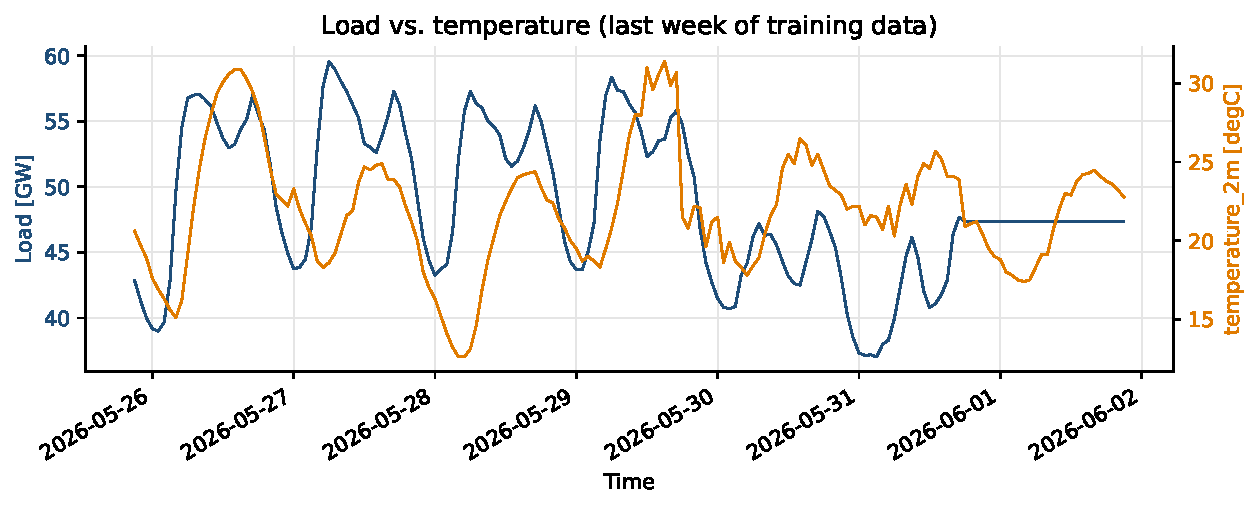
\includegraphics[keepaspectratio]{14_team_4_submission_files/figure-pdf/fig-team4-weather-output-1.pdf}}

}

\caption{\label{fig-team4-weather}Weekly overlay of temperature and load
on twin y-axes: the temperature-like weather column (orange, right axis)
against the curated \texttt{Actual\ Load} (blue, left axis). Cold spells
lift the load; mild days dampen the midday peak.}

\end{figure}%

\begin{Shaded}
\begin{Highlighting}[]
\ImportTok{import}\NormalTok{ matplotlib.pyplot }\ImportTok{as}\NormalTok{ plt}

\NormalTok{rbf\_cols }\OperatorTok{=}\NormalTok{ [c }\ControlFlowTok{for}\NormalTok{ c }\KeywordTok{in}\NormalTok{ exog\_all.columns}
            \ControlFlowTok{if} \BuiltInTok{any}\NormalTok{(k }\KeywordTok{in}\NormalTok{ c.lower() }\ControlFlowTok{for}\NormalTok{ k }\KeywordTok{in}\NormalTok{ (}\StringTok{"sin"}\NormalTok{, }\StringTok{"cos"}\NormalTok{, }\StringTok{"rbf"}\NormalTok{))]}

\ControlFlowTok{if}\NormalTok{ rbf\_cols:}
\NormalTok{    end }\OperatorTok{=}\NormalTok{ exog\_all.index.}\BuiltInTok{max}\NormalTok{()}
\NormalTok{    w }\OperatorTok{=} \BuiltInTok{slice}\NormalTok{(end }\OperatorTok{{-}}\NormalTok{ pd.Timedelta(days}\OperatorTok{=}\DecValTok{2}\NormalTok{), end)}
\NormalTok{    block }\OperatorTok{=}\NormalTok{ exog\_all.loc[w, rbf\_cols]}
\NormalTok{    fig, ax }\OperatorTok{=}\NormalTok{ plt.subplots(figsize}\OperatorTok{=}\NormalTok{(}\FloatTok{8.5}\NormalTok{, }\FloatTok{3.0}\NormalTok{))}
    \ControlFlowTok{for}\NormalTok{ c }\KeywordTok{in}\NormalTok{ rbf\_cols[:}\DecValTok{12}\NormalTok{]:}
\NormalTok{        ax.plot(block.index, block[c].values, linewidth}\OperatorTok{=}\FloatTok{0.9}\NormalTok{, alpha}\OperatorTok{=}\FloatTok{0.7}\NormalTok{)}
\NormalTok{    ax.set\_xlabel(}\StringTok{"Time"}\NormalTok{)}
\NormalTok{    ax.set\_ylabel(}\StringTok{"encoding value"}\NormalTok{)}
\NormalTok{    ax.set\_title(}\SpecialStringTok{f"Cyclical/RBF encodings (}\SpecialCharTok{\{}\BuiltInTok{len}\NormalTok{(rbf\_cols)}\SpecialCharTok{\}}\SpecialStringTok{ columns, first 12 shown)"}\NormalTok{)}
\NormalTok{    ax.grid(}\VariableTok{True}\NormalTok{, color}\OperatorTok{=}\StringTok{"\#E5E5E5"}\NormalTok{, linewidth}\OperatorTok{=}\FloatTok{0.5}\NormalTok{)}
    \ControlFlowTok{for}\NormalTok{ s }\KeywordTok{in}\NormalTok{ (}\StringTok{"top"}\NormalTok{, }\StringTok{"right"}\NormalTok{):}
\NormalTok{        ax.spines[s].set\_visible(}\VariableTok{False}\NormalTok{)}
\NormalTok{    fig.autofmt\_xdate()}
\NormalTok{    fig.tight\_layout()}
\NormalTok{    plt.show()}
\ControlFlowTok{else}\NormalTok{:}
    \BuiltInTok{print}\NormalTok{(}\StringTok{"no cyclical/RBF columns found; skipping RBF plot"}\NormalTok{)}
\end{Highlighting}
\end{Shaded}

\begin{figure}[H]

\centering{

\pandocbounded{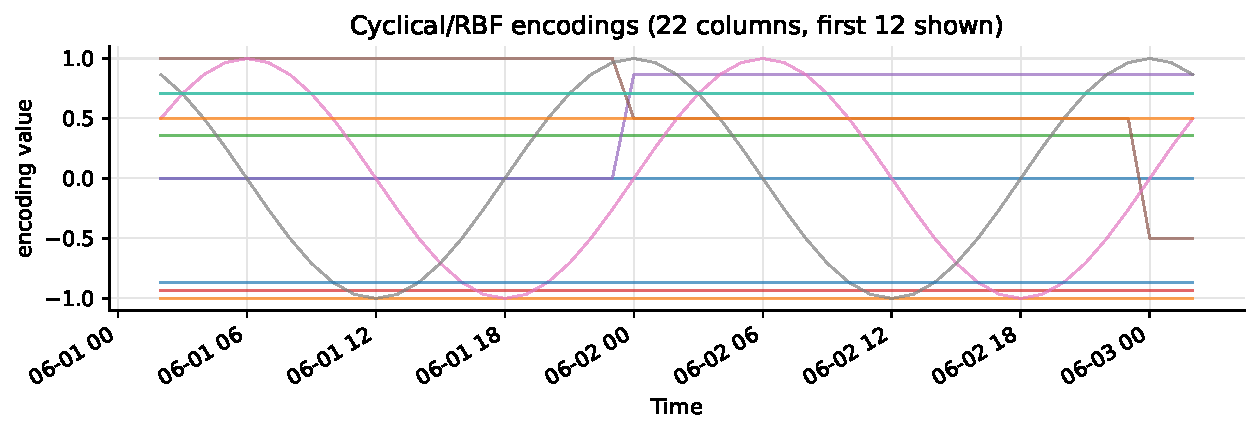
\includegraphics[keepaspectratio]{14_team_4_submission_files/figure-pdf/fig-team4-rbf-output-1.pdf}}

}

\caption{\label{fig-team4-rbf}Cyclical / radial basis function (RBF)
calendar encodings over a two-day window. Each curve is one basis
function; together they encode time-of-day and day-of-week position so
the model sees cyclic continuity across the midnight and week
boundaries.}

\end{figure}%

\begin{Shaded}
\begin{Highlighting}[]
\ImportTok{import}\NormalTok{ matplotlib.pyplot }\ImportTok{as}\NormalTok{ plt}

\NormalTok{holiday\_cols }\OperatorTok{=}\NormalTok{ [c }\ControlFlowTok{for}\NormalTok{ c }\KeywordTok{in}\NormalTok{ exog\_all.columns }\ControlFlowTok{if} \StringTok{"holiday"} \KeywordTok{in}\NormalTok{ c.lower()]}
\NormalTok{load }\OperatorTok{=}\NormalTok{ team4\_mt.df\_pipeline[}\StringTok{"Actual Load"}\NormalTok{].dropna()}

\ControlFlowTok{if}\NormalTok{ holiday\_cols }\KeywordTok{and} \BuiltInTok{len}\NormalTok{(load) }\OperatorTok{\textgreater{}} \DecValTok{0}\NormalTok{:}
\NormalTok{    hol\_col }\OperatorTok{=}\NormalTok{ holiday\_cols[}\DecValTok{0}\NormalTok{]}
\NormalTok{    hol }\OperatorTok{=}\NormalTok{ exog\_all[hol\_col]}
\NormalTok{    total\_holiday\_hours }\OperatorTok{=} \BuiltInTok{int}\NormalTok{((hol }\OperatorTok{\textgreater{}} \DecValTok{0}\NormalTok{).}\BuiltInTok{sum}\NormalTok{())}
    \BuiltInTok{print}\NormalTok{(}\SpecialStringTok{f"holiday column     : }\SpecialCharTok{\{}\NormalTok{hol\_col}\SpecialCharTok{\}}\SpecialStringTok{"}\NormalTok{)}
    \BuiltInTok{print}\NormalTok{(}\SpecialStringTok{f"total holiday hours: }\SpecialCharTok{\{}\NormalTok{total\_holiday\_hours}\SpecialCharTok{\}}\SpecialStringTok{"}\NormalTok{)}

    \CommentTok{\# Window around the most recent holiday hour, falling back to the tail.}
\NormalTok{    recent\_hol }\OperatorTok{=}\NormalTok{ hol[hol }\OperatorTok{\textgreater{}} \DecValTok{0}\NormalTok{]}
    \ControlFlowTok{if} \KeywordTok{not}\NormalTok{ recent\_hol.empty:}
\NormalTok{        center }\OperatorTok{=}\NormalTok{ recent\_hol.index.}\BuiltInTok{max}\NormalTok{()}
    \ControlFlowTok{else}\NormalTok{:}
\NormalTok{        center }\OperatorTok{=}\NormalTok{ load.index.}\BuiltInTok{max}\NormalTok{()}
\NormalTok{    w }\OperatorTok{=} \BuiltInTok{slice}\NormalTok{(center }\OperatorTok{{-}}\NormalTok{ pd.Timedelta(days}\OperatorTok{=}\DecValTok{7}\NormalTok{), center }\OperatorTok{+}\NormalTok{ pd.Timedelta(days}\OperatorTok{=}\DecValTok{3}\NormalTok{))}
\NormalTok{    load\_w }\OperatorTok{=}\NormalTok{ load.loc[load.index.isin(load.loc[w].index)]}
\NormalTok{    hol\_w }\OperatorTok{=}\NormalTok{ hol.loc[w]}

\NormalTok{    fig, ax }\OperatorTok{=}\NormalTok{ plt.subplots(figsize}\OperatorTok{=}\NormalTok{(}\FloatTok{8.5}\NormalTok{, }\FloatTok{3.0}\NormalTok{))}
\NormalTok{    ax.plot(load\_w.index, load\_w.values }\OperatorTok{/} \DecValTok{1000}\NormalTok{, color}\OperatorTok{=}\StringTok{"\#1F4E79"}\NormalTok{, linewidth}\OperatorTok{=}\FloatTok{1.0}\NormalTok{)}
\NormalTok{    in\_holiday }\OperatorTok{=}\NormalTok{ hol\_w[hol\_w }\OperatorTok{\textgreater{}} \DecValTok{0}\NormalTok{].index}
    \ControlFlowTok{for}\NormalTok{ t }\KeywordTok{in}\NormalTok{ in\_holiday:}
\NormalTok{        ax.axvspan(t, t }\OperatorTok{+}\NormalTok{ pd.Timedelta(hours}\OperatorTok{=}\DecValTok{1}\NormalTok{), color}\OperatorTok{=}\StringTok{"\#E07B00"}\NormalTok{, alpha}\OperatorTok{=}\FloatTok{0.2}\NormalTok{)}
\NormalTok{    ax.set\_xlabel(}\StringTok{"Time"}\NormalTok{)}
\NormalTok{    ax.set\_ylabel(}\StringTok{"Load [GW]"}\NormalTok{)}
\NormalTok{    ax.set\_title(}\StringTok{"Load with holiday hours shaded"}\NormalTok{)}
\NormalTok{    ax.grid(}\VariableTok{True}\NormalTok{, color}\OperatorTok{=}\StringTok{"\#E5E5E5"}\NormalTok{, linewidth}\OperatorTok{=}\FloatTok{0.5}\NormalTok{)}
    \ControlFlowTok{for}\NormalTok{ s }\KeywordTok{in}\NormalTok{ (}\StringTok{"top"}\NormalTok{, }\StringTok{"right"}\NormalTok{):}
\NormalTok{        ax.spines[s].set\_visible(}\VariableTok{False}\NormalTok{)}
\NormalTok{    fig.autofmt\_xdate()}
\NormalTok{    fig.tight\_layout()}
\NormalTok{    plt.show()}
\ControlFlowTok{else}\NormalTok{:}
    \BuiltInTok{print}\NormalTok{(}\StringTok{"no holiday column found; skipping holiday plot"}\NormalTok{)}
\end{Highlighting}
\end{Shaded}

\begin{verbatim}
holiday column     : is_holiday
total holiday hours: 1200
\end{verbatim}

\begin{figure}[H]

\centering{

\pandocbounded{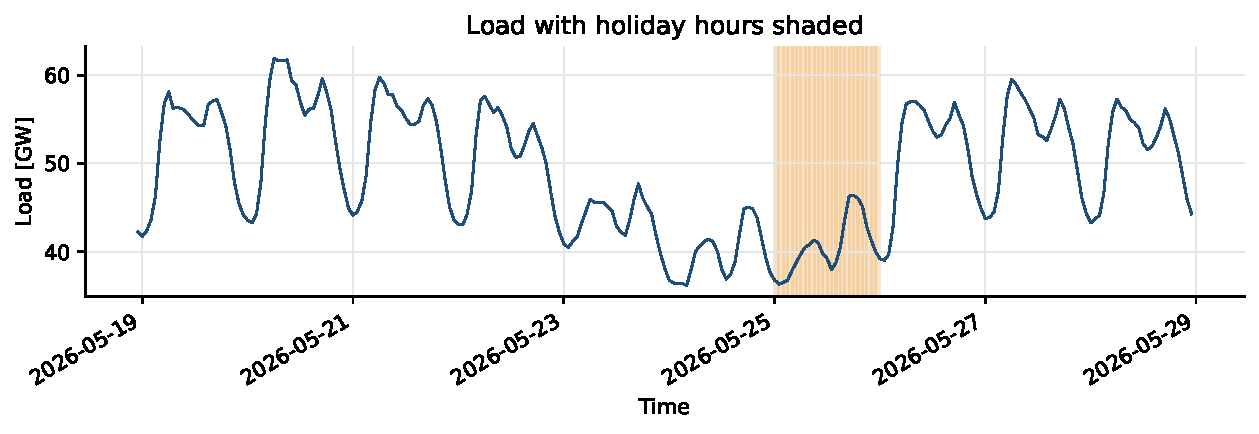
\includegraphics[keepaspectratio]{14_team_4_submission_files/figure-pdf/fig-team4-holidays-output-2.pdf}}

}

\caption{\label{fig-team4-holidays}Holiday indicator over a
representative window: the curated \texttt{Actual\ Load} with holiday
hours highlighted. Public holidays shift weekday load downward, which
the holiday feature lets the model encode.}

\end{figure}%

\begin{Shaded}
\begin{Highlighting}[]
\ImportTok{import}\NormalTok{ matplotlib.pyplot }\ImportTok{as}\NormalTok{ plt}

\CommentTok{\# With poly\_features\_degree=2 the pipeline emits poly\_\textless{}a\textgreater{}\_\_\textless{}b\textgreater{} interaction}
\CommentTok{\# columns, then keeps the top max\_poly\_features by mutual information.}
\NormalTok{poly\_cols }\OperatorTok{=}\NormalTok{ [c }\ControlFlowTok{for}\NormalTok{ c }\KeywordTok{in}\NormalTok{ exog\_all.columns }\ControlFlowTok{if}\NormalTok{ c.startswith(}\StringTok{"poly\_"}\NormalTok{)]}
\NormalTok{selected\_poly }\OperatorTok{=}\NormalTok{ [c }\ControlFlowTok{for}\NormalTok{ c }\KeywordTok{in}\NormalTok{ team4\_mt.exog\_feature\_names }\ControlFlowTok{if}\NormalTok{ c.startswith(}\StringTok{"poly\_"}\NormalTok{)]}
\BuiltInTok{print}\NormalTok{(}\SpecialStringTok{f"poly\_* columns generated : }\SpecialCharTok{\{}\BuiltInTok{len}\NormalTok{(poly\_cols)}\SpecialCharTok{\}}\SpecialStringTok{"}\NormalTok{)}
\BuiltInTok{print}\NormalTok{(}\SpecialStringTok{f"poly\_* selected (cap = }\SpecialCharTok{\{}\NormalTok{team4\_config}\SpecialCharTok{.}\NormalTok{max\_poly\_features}\SpecialCharTok{\}}\SpecialStringTok{): }\SpecialCharTok{\{}\BuiltInTok{len}\NormalTok{(selected\_poly)}\SpecialCharTok{\}}\SpecialStringTok{"}\NormalTok{)}
\ControlFlowTok{for}\NormalTok{ c }\KeywordTok{in}\NormalTok{ selected\_poly:}
    \BuiltInTok{print}\NormalTok{(}\SpecialStringTok{f"  }\SpecialCharTok{\{}\NormalTok{c}\SpecialCharTok{\}}\SpecialStringTok{"}\NormalTok{)}

\CommentTok{\# Demonstrate that a poly\_\textless{}a\textgreater{}\_\_\textless{}b\textgreater{} column equals the product of its two bases.}
\NormalTok{demonstrated }\OperatorTok{=} \VariableTok{False}
\ControlFlowTok{for}\NormalTok{ poly\_col }\KeywordTok{in}\NormalTok{ selected\_poly }\KeywordTok{or}\NormalTok{ poly\_cols:}
\NormalTok{    parts }\OperatorTok{=}\NormalTok{ poly\_col[}\BuiltInTok{len}\NormalTok{(}\StringTok{"poly\_"}\NormalTok{):].split(}\StringTok{"\_\_"}\NormalTok{)}
    \ControlFlowTok{if} \BuiltInTok{len}\NormalTok{(parts) }\OperatorTok{==} \DecValTok{2} \KeywordTok{and}\NormalTok{ parts[}\DecValTok{0}\NormalTok{] }\KeywordTok{in}\NormalTok{ exog\_all.columns }\KeywordTok{and}\NormalTok{ parts[}\DecValTok{1}\NormalTok{] }\KeywordTok{in}\NormalTok{ exog\_all.columns:}
\NormalTok{        a, b }\OperatorTok{=}\NormalTok{ parts}
\NormalTok{        product }\OperatorTok{=}\NormalTok{ exog\_all[a] }\OperatorTok{*}\NormalTok{ exog\_all[b]}
\NormalTok{        corr }\OperatorTok{=} \BuiltInTok{float}\NormalTok{(exog\_all[poly\_col].corr(product))}
        \BuiltInTok{print}\NormalTok{(}\SpecialStringTok{f"}\SpecialCharTok{\{}\NormalTok{poly\_col}\SpecialCharTok{\}}\SpecialStringTok{ == }\SpecialCharTok{\{}\NormalTok{a}\SpecialCharTok{\}}\SpecialStringTok{ * }\SpecialCharTok{\{}\NormalTok{b}\SpecialCharTok{\}}\SpecialStringTok{  (corr = }\SpecialCharTok{\{}\NormalTok{corr}\SpecialCharTok{:.4f\}}\SpecialStringTok{)"}\NormalTok{)}
\NormalTok{        fig, ax }\OperatorTok{=}\NormalTok{ plt.subplots(figsize}\OperatorTok{=}\NormalTok{(}\FloatTok{8.5}\NormalTok{, }\FloatTok{3.0}\NormalTok{))}
\NormalTok{        ax.scatter(product.values, exog\_all[poly\_col].values, s}\OperatorTok{=}\DecValTok{3}\NormalTok{, alpha}\OperatorTok{=}\FloatTok{0.3}\NormalTok{, color}\OperatorTok{=}\StringTok{"\#1F4E79"}\NormalTok{)}
\NormalTok{        ax.set\_xlabel(}\SpecialStringTok{f"}\SpecialCharTok{\{}\NormalTok{a}\SpecialCharTok{\}}\SpecialStringTok{ * }\SpecialCharTok{\{}\NormalTok{b}\SpecialCharTok{\}}\SpecialStringTok{"}\NormalTok{)}
\NormalTok{        ax.set\_ylabel(poly\_col)}
\NormalTok{        ax.set\_title(}\StringTok{"Bilinear interaction equals the product of its base features"}\NormalTok{)}
\NormalTok{        ax.grid(}\VariableTok{True}\NormalTok{, color}\OperatorTok{=}\StringTok{"\#E5E5E5"}\NormalTok{, linewidth}\OperatorTok{=}\FloatTok{0.5}\NormalTok{)}
        \ControlFlowTok{for}\NormalTok{ s }\KeywordTok{in}\NormalTok{ (}\StringTok{"top"}\NormalTok{, }\StringTok{"right"}\NormalTok{):}
\NormalTok{            ax.spines[s].set\_visible(}\VariableTok{False}\NormalTok{)}
\NormalTok{        fig.tight\_layout()}
\NormalTok{        plt.show()}
\NormalTok{        demonstrated }\OperatorTok{=} \VariableTok{True}
        \ControlFlowTok{break}
\ControlFlowTok{if} \KeywordTok{not}\NormalTok{ demonstrated:}
    \BuiltInTok{print}\NormalTok{(}\StringTok{"no recoverable poly\_\textless{}a\textgreater{}\_\_\textless{}b\textgreater{} column to demonstrate"}\NormalTok{)}

\BuiltInTok{print}\NormalTok{(}\SpecialStringTok{f"}\CharTok{\textbackslash{}n}\SpecialStringTok{\textasciigrave{}select\_exogenous\_features\textasciigrave{} pruned }\SpecialCharTok{\{}\NormalTok{exog\_all}\SpecialCharTok{.}\NormalTok{shape[}\DecValTok{1}\NormalTok{]}\SpecialCharTok{\}}\SpecialStringTok{ encoded columns "}
      \SpecialStringTok{f"down to the }\SpecialCharTok{\{}\BuiltInTok{len}\NormalTok{(team4\_mt.exog\_feature\_names)}\SpecialCharTok{\}}\SpecialStringTok{ features actually used for training."}\NormalTok{)}
\end{Highlighting}
\end{Shaded}

\begin{verbatim}
poly_* columns generated : 10
poly_* selected (cap = 10): 10
  poly_hour_cos__temperature_2m_window_1D_mean
  poly_hour_cos__temperature_2m_window_1D_max
  poly_hour_cos__temperature_2m_window_7D_mean
  poly_hour_cos__temperature_2m_window_7D_max
  poly_hour_cos__weather_code_window_7D_max
  poly_hour_cos__pressure_msl_window_7D_max
  poly_hour_cos__pressure_msl_window_7D_min
  poly_hour_cos__surface_pressure_window_7D_max
  poly_hour_cos__surface_pressure_window_7D_min
  poly_hour_cos__temperature_2m
poly_hour_cos__temperature_2m_window_1D_mean == hour_cos * temperature_2m_window_1D_mean  (corr = 1.0000)
\end{verbatim}

\begin{figure}[H]

\centering{

\pandocbounded{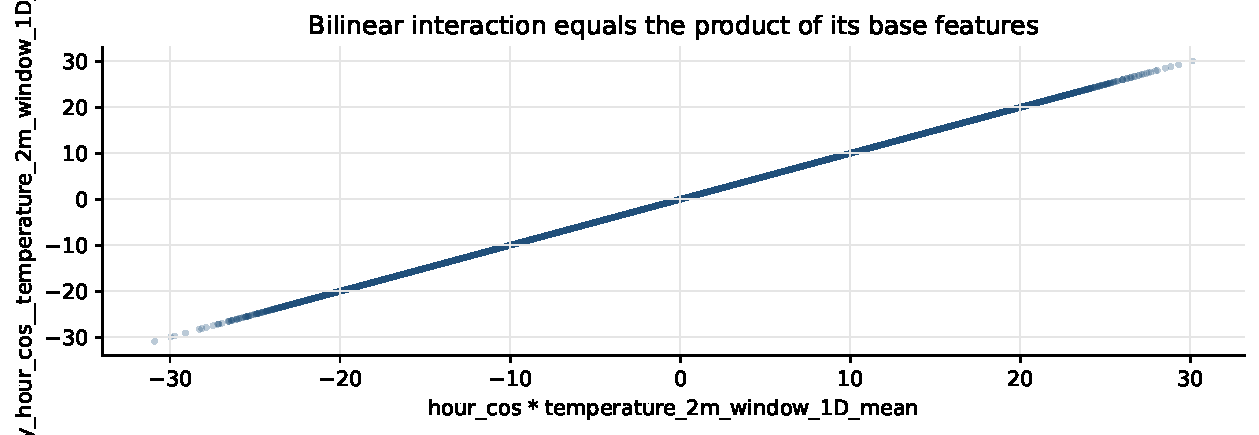
\includegraphics[keepaspectratio]{14_team_4_submission_files/figure-pdf/fig-team4-poly-output-2.pdf}}

}

\caption{\label{fig-team4-poly}Bilinear polynomial expansion produced by
the pipeline at \texttt{poly\_features\_degree=2}. Each
\texttt{poly\_\textless{}a\textgreater{}\_\_\textless{}b\textgreater{}}
column is the elementwise product of two base features; the cap keeps
only the \texttt{max\_poly\_features} most informative ones by mutual
information. The scatter confirms one such column equals the product of
its two bases (correlation ≈ 1).}

\end{figure}%

\begin{verbatim}

`select_exogenous_features` pruned 136 encoded columns down to the 127 features actually used for training.
\end{verbatim}

\subsection{Step 5 --- Train with SpotOptim and predict through
tomorrow}\label{sec-team4-run}

With the curated, gap-free target and the selected exogenous matrix in
place, \texttt{run()} executes the SpotOptim search and refits the LGBM
forecaster. With the advanced configuration this cell typically takes
5--10 minutes on a recent laptop --- mostly the SpotOptim trials against
the CV folds.

\begin{tcolorbox}[enhanced jigsaw, arc=.35mm, bottomrule=.15mm, bottomtitle=1mm, breakable, colback=white, colbacktitle=quarto-callout-note-color!10!white, colframe=quarto-callout-note-color-frame, coltitle=black, left=2mm, leftrule=.75mm, opacityback=0, opacitybacktitle=0.6, rightrule=.15mm, title=\textcolor{quarto-callout-note-color}{\faInfo}\hspace{0.5em}{Reading the SpotOptim progress bars}, titlerule=0mm, toprule=.15mm, toptitle=1mm]

Because the cell below calls \texttt{run(show=True)}, SpotOptim prints a
\texttt{tqdm} progress bar every time it scores a candidate model ---
one bar per rolling cross-validation back-test. The numbers to the right
of a finished bar, e.g.
\texttt{70/70\ {[}00:00\textless{}00:00,\ 259.84it/s{]}}, are
\texttt{tqdm}'s standard read-out:

\begin{itemize}
\tightlist
\item
  \texttt{70/70} --- steps completed out of the total; here all 70 are
  done (100 \%).
\item
  \texttt{{[}00:00\textless{}00:00,\ 259.84it/s{]}} follows the pattern
  \texttt{{[}elapsed\textless{}remaining,\ rate{]}}:

  \begin{itemize}
  \tightlist
  \item
    the first \texttt{00:00} is the wall-clock time already spent on the
    bar (\texttt{mm:ss}, or \texttt{h:mm:ss} once it passes an hour);
  \item
    the second \texttt{00:00} is \texttt{tqdm}'s estimate of the time
    still to go --- zero here, because the bar has just finished;
  \item
    \texttt{259.84it/s} is the throughput, about 260 iterations per
    second; below one per second \texttt{tqdm} switches to its
    reciprocal \texttt{s/it} (seconds per iteration).
  \end{itemize}
\end{itemize}

A bar caught mid-run,
\texttt{55/70\ {[}00:00\textless{}00:00,\ 240.00it/s{]}}, would then
read: 55 of 70 steps done, at about 240 steps per second.

The total, \texttt{70}, is the number of \emph{folds} in the back-test
that scores one candidate. The search reserves a validation span of
\texttt{delta\_val\ =\ PREDICT\_SIZE\ ×\ REFIT\_SIZE\ ×\ NUMBER\_FOLDS\ =\ 24\ ×\ 7\ ×\ 10\ =\ 1680}
hours (70 days, Section~\ref{sec-cross-validation-geometry}) and tiles
it into blocks of \texttt{cv\_block\_size} hours. The config sets
\texttt{cv\_block\_size\ =\ PREDICT\_SIZE\ =\ 24}, decoupled from the
live \texttt{predict\_size\ =\ LIVE\_N\_STEPS}
(Section~\ref{sec-team4-cutoff}), so

\[
\#\text{folds} = \frac{\texttt{delta\_val}}{\texttt{cv\_block\_size}}
              = \frac{1680}{24} = 70 .
\]

Because \texttt{cv\_block\_size} is fixed, this total is the \emph{same
on every render} --- it does not drift with the live horizon. One such
bar appears for roughly every candidate the search scores
(\texttt{n\_initial\_spotoptim\ +\ n\_trials\_spotoptim}).
Section~\ref{sec-cross-validation-geometry} derives this geometry in
full and explains why the CV block is \texttt{cv\_block\_size}, not the
live \texttt{predict\_size}.

These bars are progress reporting only. They do not affect the result.
Passing \texttt{show=False} (as Chapter~\ref{sec-live-submission} does)
suppresses them entirely.

\end{tcolorbox}

\protect\phantomsection\label{team4-train}
\begin{Shaded}
\begin{Highlighting}[]
\NormalTok{team4\_mt.run(show}\OperatorTok{=}\VariableTok{True}\NormalTok{)}

\NormalTok{future }\OperatorTok{=}\NormalTok{ team4\_mt.results[}\StringTok{"spotoptim"}\NormalTok{][}\StringTok{"Actual Load"}\NormalTok{][}\StringTok{"future\_pred"}\NormalTok{]}
\BuiltInTok{print}\NormalTok{(}\SpecialStringTok{f"raw forecast: }\SpecialCharTok{\{}\BuiltInTok{len}\NormalTok{(future)}\SpecialCharTok{\}}\SpecialStringTok{ hourly steps "}
      \SpecialStringTok{f"| }\SpecialCharTok{\{}\NormalTok{future}\SpecialCharTok{.}\NormalTok{index}\SpecialCharTok{.}\BuiltInTok{min}\NormalTok{()}\SpecialCharTok{\}}\SpecialStringTok{ → }\SpecialCharTok{\{}\NormalTok{future}\SpecialCharTok{.}\NormalTok{index}\SpecialCharTok{.}\BuiltInTok{max}\NormalTok{()}\SpecialCharTok{\}}\SpecialStringTok{"}\NormalTok{)}

\NormalTok{y0 }\OperatorTok{=}\NormalTok{ future.loc[TOMORROW\_UTC:LAST\_TARGET]}
\BuiltInTok{print}\NormalTok{(}\SpecialStringTok{f"y\_0 slice   : }\SpecialCharTok{\{}\BuiltInTok{len}\NormalTok{(y0)}\SpecialCharTok{\}}\SpecialStringTok{ hourly steps "}
      \SpecialStringTok{f"| }\SpecialCharTok{\{}\NormalTok{y0}\SpecialCharTok{.}\NormalTok{index}\SpecialCharTok{.}\BuiltInTok{min}\NormalTok{()}\SpecialCharTok{\}}\SpecialStringTok{ → }\SpecialCharTok{\{}\NormalTok{y0}\SpecialCharTok{.}\NormalTok{index}\SpecialCharTok{.}\BuiltInTok{max}\NormalTok{()}\SpecialCharTok{\}}\SpecialStringTok{"}\NormalTok{)}
\end{Highlighting}
\end{Shaded}

\begin{verbatim}
INFO:spotforecast2.multitask.base.MultiTask:Training window: 2023-06-01 18:00:00+00:00 to 2026-05-31 18:00:00+00:00
INFO:spotforecast2.multitask.base.MultiTask:[task 4] Target 'Actual Load': task 4: SpotOptim Tuned ...
INFO:spotforecast2.multitask.base.MultiTask:  Warm-start lags seeded: [1, 2, 3, 15, 24, 25, 26, 169]
\end{verbatim}

\protect\phantomsection\label{team4-train-1}
\begin{verbatim}
  0%|          | 0/70 [00:00<?, ?it/s]
\end{verbatim}

\protect\phantomsection\label{team4-train-2}
\begin{verbatim}
  0%|          | 0/70 [00:00<?, ?it/s]
\end{verbatim}

\protect\phantomsection\label{team4-train-3}
\begin{verbatim}
  0%|          | 0/70 [00:00<?, ?it/s]
\end{verbatim}

\protect\phantomsection\label{team4-train-4}
\begin{verbatim}
  0%|          | 0/70 [00:00<?, ?it/s]
\end{verbatim}

\protect\phantomsection\label{team4-train-5}
\begin{verbatim}
  0%|          | 0/70 [00:00<?, ?it/s]
\end{verbatim}

\protect\phantomsection\label{team4-train-6}
\begin{verbatim}
  0%|          | 0/70 [00:00<?, ?it/s]
\end{verbatim}

\protect\phantomsection\label{team4-train-7}
\begin{verbatim}
  0%|          | 0/70 [00:00<?, ?it/s]
\end{verbatim}

\protect\phantomsection\label{team4-train-8}
\begin{verbatim}
  0%|          | 0/70 [00:00<?, ?it/s]
\end{verbatim}

\protect\phantomsection\label{team4-train-9}
\begin{verbatim}
  0%|          | 0/70 [00:00<?, ?it/s]
\end{verbatim}

\protect\phantomsection\label{team4-train-10}
\begin{verbatim}
  0%|          | 0/70 [00:00<?, ?it/s]
\end{verbatim}

\protect\phantomsection\label{team4-train-11}
\begin{verbatim}
  0%|          | 0/70 [00:00<?, ?it/s]
\end{verbatim}

\protect\phantomsection\label{team4-train-12}
\begin{verbatim}
  0%|          | 0/70 [00:00<?, ?it/s]
\end{verbatim}

\protect\phantomsection\label{team4-train-13}
\begin{verbatim}
  0%|          | 0/70 [00:00<?, ?it/s]
\end{verbatim}

\protect\phantomsection\label{team4-train-14}
\begin{verbatim}
  0%|          | 0/70 [00:00<?, ?it/s]
\end{verbatim}

\protect\phantomsection\label{team4-train-15}
\begin{verbatim}
  0%|          | 0/70 [00:00<?, ?it/s]
\end{verbatim}

\protect\phantomsection\label{team4-train-16}
\begin{verbatim}
  0%|          | 0/70 [00:00<?, ?it/s]
\end{verbatim}

\protect\phantomsection\label{team4-train-17}
\begin{verbatim}
  0%|          | 0/70 [00:00<?, ?it/s]
\end{verbatim}

\protect\phantomsection\label{team4-train-18}
\begin{verbatim}
  0%|          | 0/70 [00:00<?, ?it/s]
\end{verbatim}

\protect\phantomsection\label{team4-train-19}
\begin{verbatim}
  0%|          | 0/70 [00:00<?, ?it/s]
\end{verbatim}

\protect\phantomsection\label{team4-train-20}
\begin{verbatim}
  0%|          | 0/70 [00:00<?, ?it/s]
\end{verbatim}

\protect\phantomsection\label{team4-train-21}
\begin{verbatim}
  0%|          | 0/70 [00:00<?, ?it/s]
\end{verbatim}

\protect\phantomsection\label{team4-train-22}
\begin{verbatim}
  0%|          | 0/70 [00:00<?, ?it/s]
\end{verbatim}

\protect\phantomsection\label{team4-train-23}
\begin{verbatim}
  0%|          | 0/70 [00:00<?, ?it/s]
\end{verbatim}

\protect\phantomsection\label{team4-train-24}
\begin{verbatim}
  0%|          | 0/70 [00:00<?, ?it/s]
\end{verbatim}

\protect\phantomsection\label{team4-train-25}
\begin{verbatim}
  0%|          | 0/70 [00:00<?, ?it/s]
\end{verbatim}

\protect\phantomsection\label{team4-train-26}
\begin{verbatim}
  0%|          | 0/70 [00:00<?, ?it/s]
\end{verbatim}

\protect\phantomsection\label{team4-train-27}
\begin{verbatim}
  0%|          | 0/70 [00:00<?, ?it/s]
\end{verbatim}

\protect\phantomsection\label{team4-train-28}
\begin{verbatim}
  0%|          | 0/70 [00:00<?, ?it/s]
\end{verbatim}

\protect\phantomsection\label{team4-train-29}
\begin{verbatim}
  0%|          | 0/70 [00:00<?, ?it/s]
\end{verbatim}

\protect\phantomsection\label{team4-train-30}
\begin{verbatim}
  0%|          | 0/70 [00:00<?, ?it/s]
\end{verbatim}

\begin{verbatim}
INFO:spotforecast2.multitask.base.MultiTask:  Best params: {'estimator__num_leaves': 122, 'estimator__max_depth': 5, 'estimator__learning_rate': 0.04439790498017541, 'estimator__n_estimators': 1000, 'estimator__bagging_fraction': 0.5536051912008192, 'estimator__feature_fraction': 0.9774780308571953, 'estimator__reg_alpha': 79.19710044140665, 'estimator__reg_lambda': 20.718186181635744}
INFO:spotforecast2.multitask.base.MultiTask:  Best lags: [ 1  2 23 24 47 48]
INFO:spotforecast2.multitask.base.MultiTask:  Saved tuning results: /Users/bartz/.spotforecast2_cache/ddmo_ch14_team4/tuning_results/ddmo-live-team4_Actual Load_spotoptim_20260531_195113.json
\end{verbatim}

\begin{verbatim}
`Forecaster` refitted using the best-found lags and parameters, and the whole data set: 
  Lags: [ 1  2 23 24 47 48] 
  Parameters: {'estimator__num_leaves': 122, 'estimator__max_depth': 5, 'estimator__learning_rate': 0.04439790498017541, 'estimator__n_estimators': 1000, 'estimator__bagging_fraction': 0.5536051912008192, 'estimator__feature_fraction': 0.9774780308571953, 'estimator__reg_alpha': 79.19710044140665, 'estimator__reg_lambda': 20.718186181635744}
  Backtesting metric: 1935.868793601971
\end{verbatim}

\protect\phantomsection\label{team4-train-31}
\begin{verbatim}
Unable to display output for mime type(s): text/html
\end{verbatim}

\begin{verbatim}
INFO:spotforecast2.multitask.base.MultiTask:  Saved model: /Users/bartz/.spotforecast2_cache/ddmo_ch14_team4/models/ddmo-live-team4/ddmo-live-team4_Actual Load_spotoptim_20260531_195118.joblib
\end{verbatim}

\begin{verbatim}
raw forecast: 29 hourly steps | 2026-05-31 19:00:00+00:00 → 2026-06-01 23:00:00+00:00
y_0 slice   : 24 hourly steps | 2026-06-01 00:00:00+00:00 → 2026-06-01 23:00:00+00:00
\end{verbatim}

\subsection{Step 6 --- Feature importance and
SHAP}\label{sec-team4-importance}

The fitted forecaster lives in the results dict. We reconstruct its
training design matrix --- lags plus selected exogenous features --- and
read two complementary attributions: LightGBM's split-count importance
and SHapley Additive exPlanations (SHAP). Both answer the Art. 13
transparency question \emph{what does the model base its forecast on?}
The cell also asserts a key data-governance invariant: ENTSO-E's own
\texttt{Forecasted\ Load} is held out as test data and never enters the
model --- only the post-processing comparison in
Section~\ref{sec-team4-vs-entsoe} may read it.

\protect\phantomsection\label{team4-load-model}
\begin{Shaded}
\begin{Highlighting}[]
\NormalTok{fc }\OperatorTok{=}\NormalTok{ team4\_mt.results[}\StringTok{"spotoptim"}\NormalTok{][}\StringTok{"Actual Load"}\NormalTok{][}\StringTok{"forecaster"}\NormalTok{]}

\NormalTok{X\_tr, y\_int }\OperatorTok{=}\NormalTok{ fc.create\_train\_X\_y(}
\NormalTok{    y}\OperatorTok{=}\NormalTok{team4\_mt.data\_with\_exog[}\StringTok{"Actual Load"}\NormalTok{],}
\NormalTok{    exog}\OperatorTok{=}\NormalTok{team4\_mt.data\_with\_exog[team4\_mt.exog\_feature\_names],}
\NormalTok{)}
\ControlFlowTok{assert} \BuiltInTok{list}\NormalTok{(X\_tr.columns) }\OperatorTok{==} \BuiltInTok{list}\NormalTok{(fc.estimator.feature\_name\_), }\OperatorTok{\textbackslash{}}
    \StringTok{"design{-}matrix columns do not match the fitted estimator\textquotesingle{}s feature names"}

\NormalTok{feat\_names }\OperatorTok{=} \BuiltInTok{list}\NormalTok{(fc.estimator.feature\_name\_)}
\BuiltInTok{print}\NormalTok{(}\SpecialStringTok{f"trained features: }\SpecialCharTok{\{}\BuiltInTok{len}\NormalTok{(feat\_names)}\SpecialCharTok{\}}\SpecialStringTok{"}\NormalTok{)}

\CommentTok{\# Safety invariant (CR{-}3): ENTSO{-}E\textquotesingle{}s own day{-}ahead forecast must NEVER reach}
\CommentTok{\# the model. It is neither a target nor a selected exogenous feature, so}
\CommentTok{\# \textasciigrave{}merge\_data\_and\_covariates\textasciigrave{} drops it before training {-}{-}{-} we assert that}
\CommentTok{\# here, fail{-}loud, so any future regression that let it leak would break the}
\CommentTok{\# render rather than silently bias the model.}
\NormalTok{LEAKAGE\_COLS }\OperatorTok{=}\NormalTok{ \{}\StringTok{"Forecasted Load"}\NormalTok{, }\StringTok{"Actual"}\NormalTok{\}}
\ControlFlowTok{assert} \KeywordTok{not}\NormalTok{ (LEAKAGE\_COLS }\OperatorTok{\&} \BuiltInTok{set}\NormalTok{(team4\_mt.data\_with\_exog.columns)), }\OperatorTok{\textbackslash{}}
    \StringTok{"ENTSO{-}E forecast leaked into the training frame (data\_with\_exog)!"}
\ControlFlowTok{assert} \KeywordTok{not}\NormalTok{ (LEAKAGE\_COLS }\OperatorTok{\&} \BuiltInTok{set}\NormalTok{(team4\_mt.exog\_feature\_names)), }\OperatorTok{\textbackslash{}}
    \StringTok{"ENTSO{-}E forecast leaked into the selected exogenous features!"}
\ControlFlowTok{assert} \KeywordTok{not}\NormalTok{ (LEAKAGE\_COLS }\OperatorTok{\&} \BuiltInTok{set}\NormalTok{(feat\_names)), }\OperatorTok{\textbackslash{}}
    \StringTok{"ENTSO{-}E forecast leaked into the fitted model\textquotesingle{}s features!"}
\BuiltInTok{print}\NormalTok{(}\StringTok{"leakage guard passed: ENTSO{-}E forecast absent from target, exog, and model features"}\NormalTok{)}

\NormalTok{fam\_counts }\OperatorTok{=}\NormalTok{ \{\}}
\ControlFlowTok{for}\NormalTok{ col }\KeywordTok{in}\NormalTok{ feat\_names:}
\NormalTok{    fam\_counts[family\_of(col)] }\OperatorTok{=}\NormalTok{ fam\_counts.get(family\_of(col), }\DecValTok{0}\NormalTok{) }\OperatorTok{+} \DecValTok{1}
\ControlFlowTok{for}\NormalTok{ fam, n }\KeywordTok{in} \BuiltInTok{sorted}\NormalTok{(fam\_counts.items(), key}\OperatorTok{=}\KeywordTok{lambda}\NormalTok{ kv: kv[}\DecValTok{1}\NormalTok{], reverse}\OperatorTok{=}\VariableTok{True}\NormalTok{):}
    \BuiltInTok{print}\NormalTok{(}\SpecialStringTok{f"  }\SpecialCharTok{\{}\NormalTok{fam}\SpecialCharTok{:\textless{}16\}}\SpecialStringTok{: }\SpecialCharTok{\{}\NormalTok{n}\SpecialCharTok{\}}\SpecialStringTok{"}\NormalTok{)}
\end{Highlighting}
\end{Shaded}

\begin{verbatim}
trained features: 134
leakage guard passed: ENTSO-E forecast absent from target, exog, and model features
  weather_window  : 90
  weather/other   : 16
  cyclical/RBF    : 12
  polynomial      : 10
  lag             : 6
\end{verbatim}

\begin{Shaded}
\begin{Highlighting}[]
\ImportTok{import}\NormalTok{ matplotlib.pyplot }\ImportTok{as}\NormalTok{ plt}

\NormalTok{importances }\OperatorTok{=}\NormalTok{ fc.estimator.feature\_importances\_}
\NormalTok{ranking }\OperatorTok{=} \BuiltInTok{sorted}\NormalTok{(}\BuiltInTok{zip}\NormalTok{(feat\_names, importances), key}\OperatorTok{=}\KeywordTok{lambda}\NormalTok{ kv: kv[}\DecValTok{1}\NormalTok{], reverse}\OperatorTok{=}\VariableTok{True}\NormalTok{)[:}\DecValTok{20}\NormalTok{]}

\NormalTok{family\_color }\OperatorTok{=}\NormalTok{ \{}
    \StringTok{"lag"}\NormalTok{:            }\StringTok{"\#B22222"}\NormalTok{,}
    \StringTok{"weather/other"}\NormalTok{:  }\StringTok{"\#E07B00"}\NormalTok{,}
    \StringTok{"weather\_window"}\NormalTok{: }\StringTok{"\#F0A33C"}\NormalTok{,}
    \StringTok{"cyclical/RBF"}\NormalTok{:   }\StringTok{"\#1F4E79"}\NormalTok{,}
    \StringTok{"holiday"}\NormalTok{:        }\StringTok{"\#2E8B57"}\NormalTok{,}
    \StringTok{"polynomial"}\NormalTok{:     }\StringTok{"\#7B5EA7"}\NormalTok{,}
\NormalTok{\}}

\NormalTok{labels }\OperatorTok{=}\NormalTok{ [n }\ControlFlowTok{for}\NormalTok{ n, \_ }\KeywordTok{in}\NormalTok{ ranking][::}\OperatorTok{{-}}\DecValTok{1}\NormalTok{]}
\NormalTok{values }\OperatorTok{=}\NormalTok{ [v }\ControlFlowTok{for}\NormalTok{ \_, v }\KeywordTok{in}\NormalTok{ ranking][::}\OperatorTok{{-}}\DecValTok{1}\NormalTok{]}
\NormalTok{colors }\OperatorTok{=}\NormalTok{ [family\_color.get(family\_of(n), }\StringTok{"\#888888"}\NormalTok{) }\ControlFlowTok{for}\NormalTok{ n }\KeywordTok{in}\NormalTok{ labels]}

\NormalTok{fig, ax }\OperatorTok{=}\NormalTok{ plt.subplots(figsize}\OperatorTok{=}\NormalTok{(}\FloatTok{8.5}\NormalTok{, }\FloatTok{5.5}\NormalTok{))}
\NormalTok{ax.barh(labels, values, color}\OperatorTok{=}\NormalTok{colors)}
\NormalTok{ax.set\_xlabel(}\StringTok{"split count (feature importance)"}\NormalTok{)}
\NormalTok{ax.set\_title(}\StringTok{"Top{-}20 feature importances (coloured by family; lags in red)"}\NormalTok{)}
\NormalTok{ax.grid(}\VariableTok{True}\NormalTok{, axis}\OperatorTok{=}\StringTok{"x"}\NormalTok{, color}\OperatorTok{=}\StringTok{"\#E5E5E5"}\NormalTok{, linewidth}\OperatorTok{=}\FloatTok{0.5}\NormalTok{)}
\NormalTok{handles }\OperatorTok{=}\NormalTok{ [plt.Rectangle((}\DecValTok{0}\NormalTok{, }\DecValTok{0}\NormalTok{), }\DecValTok{1}\NormalTok{, }\DecValTok{1}\NormalTok{, color}\OperatorTok{=}\NormalTok{c) }\ControlFlowTok{for}\NormalTok{ c }\KeywordTok{in}\NormalTok{ family\_color.values()]}
\NormalTok{ax.legend(handles, family\_color.keys(), fontsize}\OperatorTok{=}\DecValTok{7}\NormalTok{, loc}\OperatorTok{=}\StringTok{"lower right"}\NormalTok{)}
\ControlFlowTok{for}\NormalTok{ s }\KeywordTok{in}\NormalTok{ (}\StringTok{"top"}\NormalTok{, }\StringTok{"right"}\NormalTok{):}
\NormalTok{    ax.spines[s].set\_visible(}\VariableTok{False}\NormalTok{)}
\NormalTok{fig.tight\_layout()}
\NormalTok{plt.show()}
\end{Highlighting}
\end{Shaded}

\begin{figure}[H]

\centering{

\pandocbounded{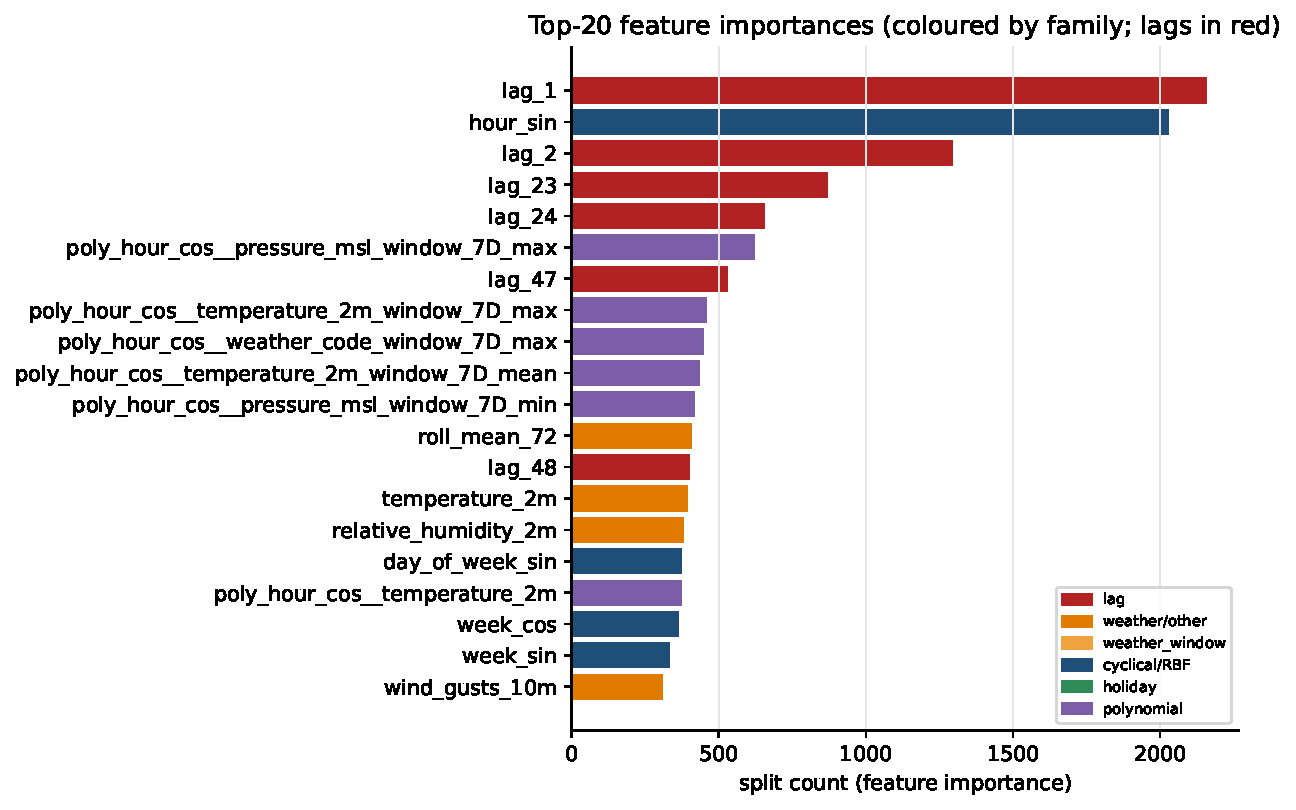
\includegraphics[keepaspectratio]{14_team_4_submission_files/figure-pdf/fig-team4-importance-output-1.pdf}}

}

\caption{\label{fig-team4-importance}Top-20 LightGBM split-count feature
importances of the tuned forecaster, coloured by feature family. Lag
features (highlighted) carry the bulk of the information; weather,
calendar, holiday, and polynomial features supplement them.}

\end{figure}%

\begin{Shaded}
\begin{Highlighting}[]
\ImportTok{import}\NormalTok{ shap}
\ImportTok{import}\NormalTok{ matplotlib.pyplot }\ImportTok{as}\NormalTok{ plt}

\NormalTok{step }\OperatorTok{=} \BuiltInTok{max}\NormalTok{(}\DecValTok{1}\NormalTok{, }\BuiltInTok{len}\NormalTok{(X\_tr) }\OperatorTok{//} \DecValTok{2000}\NormalTok{)}
\NormalTok{X\_sample }\OperatorTok{=}\NormalTok{ X\_tr.iloc[::step]}

\NormalTok{explainer }\OperatorTok{=}\NormalTok{ shap.TreeExplainer(fc.estimator)}
\NormalTok{sv }\OperatorTok{=}\NormalTok{ explainer.shap\_values(X\_sample)}

\NormalTok{shap.summary\_plot(sv, X\_sample, plot\_type}\OperatorTok{=}\StringTok{"bar"}\NormalTok{, show}\OperatorTok{=}\VariableTok{False}\NormalTok{)}
\NormalTok{plt.tight\_layout()}
\NormalTok{plt.show()}
\end{Highlighting}
\end{Shaded}

\begin{figure}[H]

\centering{

\pandocbounded{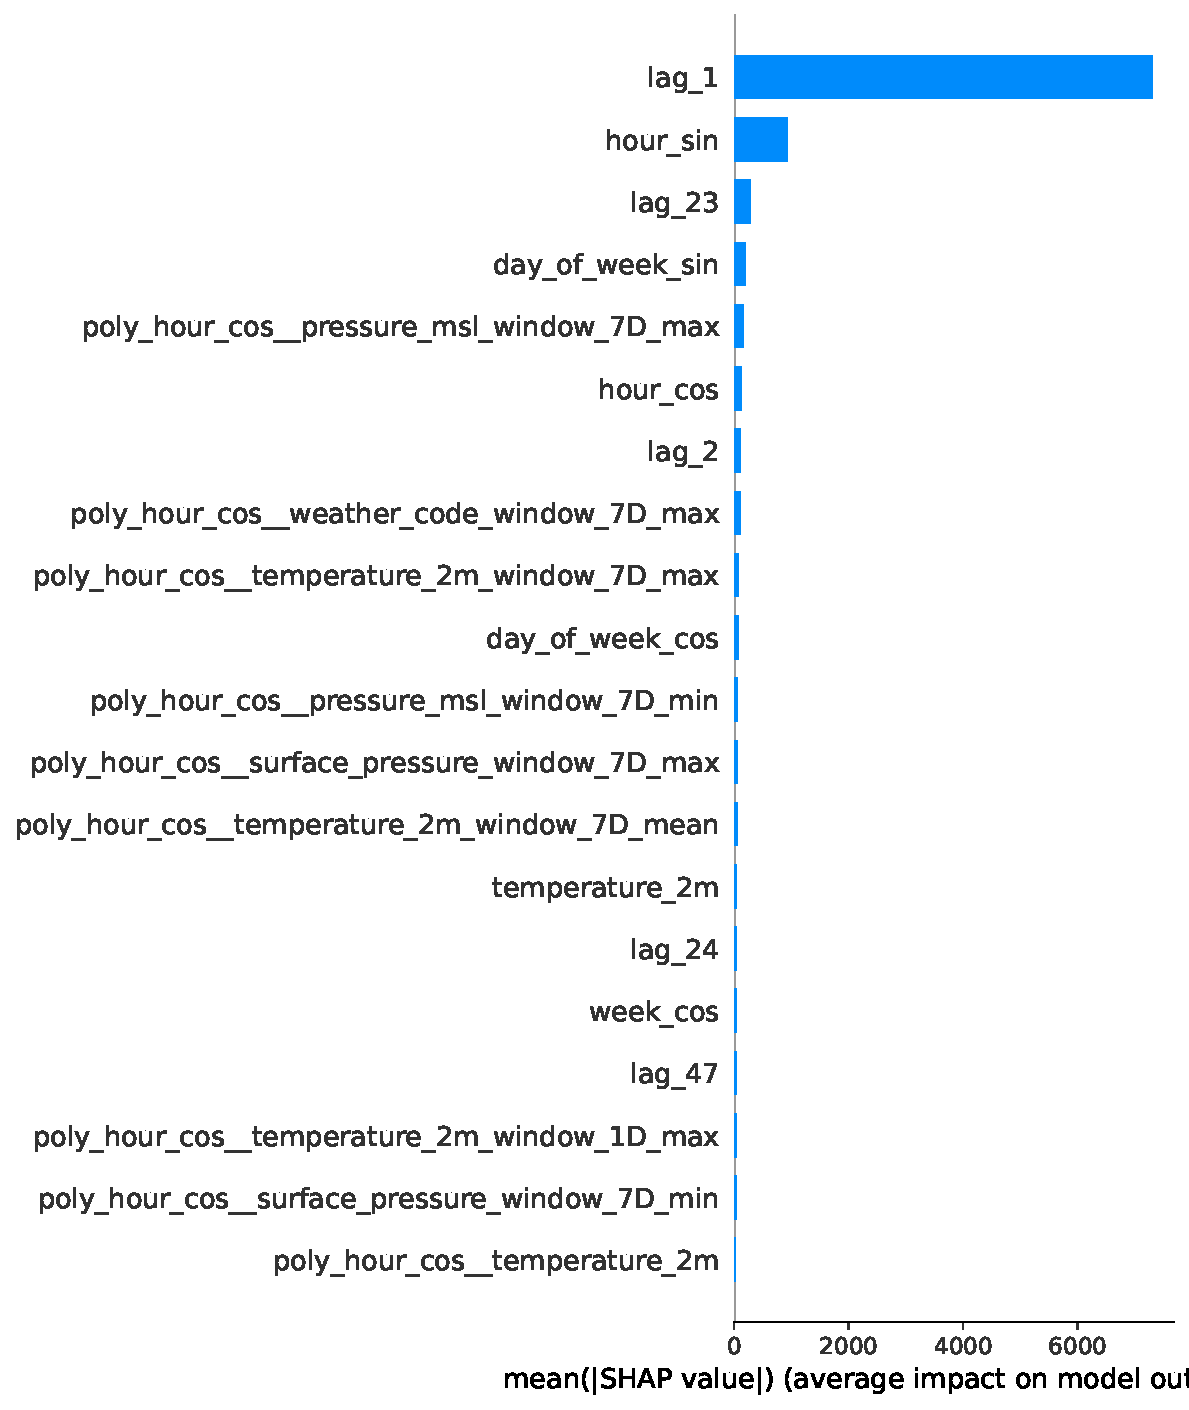
\includegraphics[keepaspectratio]{14_team_4_submission_files/figure-pdf/fig-team4-shap-output-1.pdf}}

}

\caption{\label{fig-team4-shap}Mean absolute SHapley Additive
exPlanations (SHAP) value per feature over a ≈2000-row deterministic
sample of the training design matrix. SHAP measures each feature's
average contribution to the prediction, complementing the split-count
ranking above.}

\end{figure}%

Split-count importance ranks features by how often LightGBM branches on
them, while mean absolute SHAP ranks them by their average effect on the
forecast --- the two orderings can disagree, and reporting both is the
kind of layered explanation Art. 13 transparency expects.

\subsection{Visual inspection}\label{visual-inspection-1}

\texttt{make\_plot} (its \texttt{PredictionFigure} builder) already
knows how to draw a benchmark line: whenever the prediction package
carries a \texttt{future\_forecast} Series, the figure adds a
``Benchmark Forecast (e.g., ENTSOE)'' trace for free. So overlaying
ENTSO-E's own day-ahead forecast is a one-liner --- assign
\texttt{predictions\_entsoe}
(Section~\ref{sec-team4-entsoe-predictions}) to that key before calling
\texttt{make\_plot}, rather than appending a Plotly trace by hand. The
series must be in raw MW (the same units \texttt{future\_pred} uses) and
is reindexed onto the forecast horizon so it lines up hour-for-hour. The
benchmark legend also reads optional \texttt{metrics\_forecast} /
\texttt{metrics\_forecast\_one\_day} entries; we leave them unset ---
the target day is not yet scorable (Section~\ref{sec-team4-vs-entsoe})
--- so those MAE/MAPE figures render as zero placeholders until the
actuals arrive.

\begin{Shaded}
\begin{Highlighting}[]
\ImportTok{from}\NormalTok{ spotforecast2.plots.plotter }\ImportTok{import}\NormalTok{ make\_plot}

\NormalTok{pkg }\OperatorTok{=}\NormalTok{ team4\_mt.results[}\StringTok{"spotoptim"}\NormalTok{][}\StringTok{"Actual Load"}\NormalTok{]}

\CommentTok{\# Built{-}in benchmark trace: PredictionFigure draws a "Benchmark Forecast" line}
\CommentTok{\# whenever the package carries a \textasciigrave{}future\_forecast\textasciigrave{} Series (raw MW, like}
\CommentTok{\# \textasciigrave{}future\_pred\textasciigrave{}). Reuse predictions\_entsoe, reindexed onto the forecast horizon.}
\NormalTok{pkg[}\StringTok{"future\_forecast"}\NormalTok{] }\OperatorTok{=}\NormalTok{ predictions\_entsoe.reindex(pkg[}\StringTok{"future\_pred"}\NormalTok{].index)}

\BuiltInTok{print}\NormalTok{(}\StringTok{"future\_pred     :"}\NormalTok{, }\BuiltInTok{len}\NormalTok{(pkg[}\StringTok{"future\_pred"}\NormalTok{]), }\StringTok{"rows,"}\NormalTok{,}
\NormalTok{      pkg[}\StringTok{"future\_pred"}\NormalTok{].index.}\BuiltInTok{min}\NormalTok{(), }\StringTok{"→"}\NormalTok{, pkg[}\StringTok{"future\_pred"}\NormalTok{].index.}\BuiltInTok{max}\NormalTok{())}
\BuiltInTok{print}\NormalTok{(}\StringTok{"future\_forecast :"}\NormalTok{, }\BuiltInTok{int}\NormalTok{(pkg[}\StringTok{"future\_forecast"}\NormalTok{].notna().}\BuiltInTok{sum}\NormalTok{()),}
      \StringTok{"of"}\NormalTok{, }\BuiltInTok{len}\NormalTok{(pkg[}\StringTok{"future\_forecast"}\NormalTok{]), }\StringTok{"ENTSO{-}E hours populated"}\NormalTok{)}
\BuiltInTok{print}\NormalTok{(}\StringTok{"metrics\_future         :"}\NormalTok{, pkg.get(}\StringTok{"metrics\_future"}\NormalTok{))}
\BuiltInTok{print}\NormalTok{(}\StringTok{"metrics\_future\_one\_day :"}\NormalTok{, pkg.get(}\StringTok{"metrics\_future\_one\_day"}\NormalTok{))}

\NormalTok{fig }\OperatorTok{=}\NormalTok{ make\_plot(pkg)}
\NormalTok{fig.show()}
\end{Highlighting}
\end{Shaded}

\begin{verbatim}
future_pred     : 29 rows, 2026-05-31 19:00:00+00:00 → 2026-06-01 23:00:00+00:00
future_forecast : 27 of 29 ENTSO-E hours populated
metrics_future         : {}
metrics_future_one_day : {}
\end{verbatim}

\begin{figure}

\centering{

\begin{verbatim}
Unable to display output for mime type(s): text/html
\end{verbatim}

}

\caption{\label{fig-team4-predict}team\_4 live ENTSO-E DE load forecast
--- advanced setup (6 SpotOptim trials, 5 seasonal periods, weather
windows, holiday and polynomial features). Training fit left of the
dashed line; recursive forecast through tomorrow 23:00 UTC right of it.
The 24 hourly values for \texttt{y\_0} are the rightmost block. The
benchmark trace is ENTSO-E's own day-ahead \texttt{Forecasted\ Load}, an
independent baseline the model never trains on
(Section~\ref{sec-team4-entsoe-predictions}).}

\end{figure}%

\subsection{ENTSO-E's own day-ahead forecast
vs.~ours}\label{sec-team4-vs-entsoe}

ENTSO-E publishes a day-ahead \texttt{Forecasted\ Load} alongside the
actuals (Section~\ref{sec-team4-prepare}). The model never uses it ---
it is neither the target nor an exogenous feature --- but it is a free,
independent baseline: the transmission system operators' own prediction
for the same 24 hours. The cell below restricts
\texttt{predictions\_entsoe}
(Section~\ref{sec-team4-entsoe-predictions}) to \texttt{y\_0}'s window
and overlays it on \texttt{team\_4}'s forecast. Neither curve can be
scored yet (the target day's actuals are not observed), so this is a
forecast-vs-forecast comparison; the printed mean absolute difference
quantifies how far the two disagree. The day-ahead forecast reaches the
interim file because the download in Section~\ref{sec-team4-download}
passes \texttt{keep\_forecast\_future=True} (without it,
\texttt{download\_new\_data} drops every future row). It is published
around midday \texttt{D-1}, so a render before that window --- or the
last UTC hours of the target day, which fall into the next local
publication day --- may leave a few target hours uncovered; the cell
handles that gracefully and draws only the hours ENTSO-E has actually
published.

\begin{Shaded}
\begin{Highlighting}[]
\ImportTok{import}\NormalTok{ matplotlib.pyplot }\ImportTok{as}\NormalTok{ plt}

\CommentTok{\# Reuse predictions\_entsoe (@sec{-}team4{-}entsoe{-}predictions) {-}{-}{-} already on the}
\CommentTok{\# hourly grid {-}{-}{-} restricted to y\_0\textquotesingle{}s 24{-}hour window.}
\NormalTok{entsoe\_fc }\OperatorTok{=}\NormalTok{ predictions\_entsoe.reindex(y0.index)}
\NormalTok{overlap }\OperatorTok{=}\NormalTok{ entsoe\_fc.dropna().index}
\BuiltInTok{print}\NormalTok{(}\SpecialStringTok{f"ENTSO{-}E day{-}ahead hours available on target day: }\SpecialCharTok{\{}\BuiltInTok{len}\NormalTok{(overlap)}\SpecialCharTok{\}}\SpecialStringTok{ / }\SpecialCharTok{\{}\BuiltInTok{len}\NormalTok{(y0)}\SpecialCharTok{\}}\SpecialStringTok{"}\NormalTok{)}
\ControlFlowTok{if} \BuiltInTok{len}\NormalTok{(overlap) }\OperatorTok{\textgreater{}} \DecValTok{0}\NormalTok{:}
\NormalTok{    mad }\OperatorTok{=} \BuiltInTok{float}\NormalTok{((y0.loc[overlap] }\OperatorTok{{-}}\NormalTok{ entsoe\_fc.loc[overlap]).}\BuiltInTok{abs}\NormalTok{().mean())}
    \BuiltInTok{print}\NormalTok{(}\SpecialStringTok{f"mean |team\_4 {-} ENTSO{-}E| over the overlap: }\SpecialCharTok{\{}\NormalTok{mad}\SpecialCharTok{:,.0f\}}\SpecialStringTok{ MW"}\NormalTok{)}
\ControlFlowTok{else}\NormalTok{:}
    \BuiltInTok{print}\NormalTok{(}\StringTok{"ENTSO{-}E has not published a day{-}ahead forecast for the target day "}
          \StringTok{"in the local cache yet; showing team\_4 only."}\NormalTok{)}

\NormalTok{fig, ax }\OperatorTok{=}\NormalTok{ plt.subplots(figsize}\OperatorTok{=}\NormalTok{(}\FloatTok{8.5}\NormalTok{, }\FloatTok{3.5}\NormalTok{))}
\NormalTok{ax.plot(y0.index, y0.values }\OperatorTok{/} \DecValTok{1000}\NormalTok{, marker}\OperatorTok{=}\StringTok{"o"}\NormalTok{, ms}\OperatorTok{=}\DecValTok{3}\NormalTok{, color}\OperatorTok{=}\StringTok{"\#1F4E79"}\NormalTok{,}
\NormalTok{        label}\OperatorTok{=}\StringTok{"team\_4 forecast (y\_0)"}\NormalTok{)}
\ControlFlowTok{if} \BuiltInTok{len}\NormalTok{(overlap) }\OperatorTok{\textgreater{}} \DecValTok{0}\NormalTok{:}
\NormalTok{    ax.plot(entsoe\_fc.index, entsoe\_fc.values }\OperatorTok{/} \DecValTok{1000}\NormalTok{, marker}\OperatorTok{=}\StringTok{"x"}\NormalTok{, ms}\OperatorTok{=}\DecValTok{4}\NormalTok{,}
\NormalTok{            color}\OperatorTok{=}\StringTok{"\#E07B00"}\NormalTok{, label}\OperatorTok{=}\StringTok{"ENTSO{-}E day{-}ahead forecast"}\NormalTok{)}
\NormalTok{ax.set\_xlabel(}\StringTok{"Time (UTC)"}\NormalTok{)}
\NormalTok{ax.set\_ylabel(}\StringTok{"Load [GW]"}\NormalTok{)}
\NormalTok{ax.set\_title(}\StringTok{"team\_4 vs. ENTSO{-}E day{-}ahead forecast {-}{-}{-} target day"}\NormalTok{)}
\NormalTok{ax.grid(}\VariableTok{True}\NormalTok{, color}\OperatorTok{=}\StringTok{"\#E5E5E5"}\NormalTok{, linewidth}\OperatorTok{=}\FloatTok{0.5}\NormalTok{)}
\NormalTok{ax.legend(fontsize}\OperatorTok{=}\DecValTok{8}\NormalTok{)}
\ControlFlowTok{for}\NormalTok{ s }\KeywordTok{in}\NormalTok{ (}\StringTok{"top"}\NormalTok{, }\StringTok{"right"}\NormalTok{):}
\NormalTok{    ax.spines[s].set\_visible(}\VariableTok{False}\NormalTok{)}
\NormalTok{fig.autofmt\_xdate()}
\NormalTok{fig.tight\_layout()}
\NormalTok{plt.show()}
\end{Highlighting}
\end{Shaded}

\begin{verbatim}
ENTSO-E day-ahead hours available on target day: 22 / 24
mean |team_4 - ENTSO-E| over the overlap: 4,988 MW
\end{verbatim}

\begin{figure}[H]

\centering{

\pandocbounded{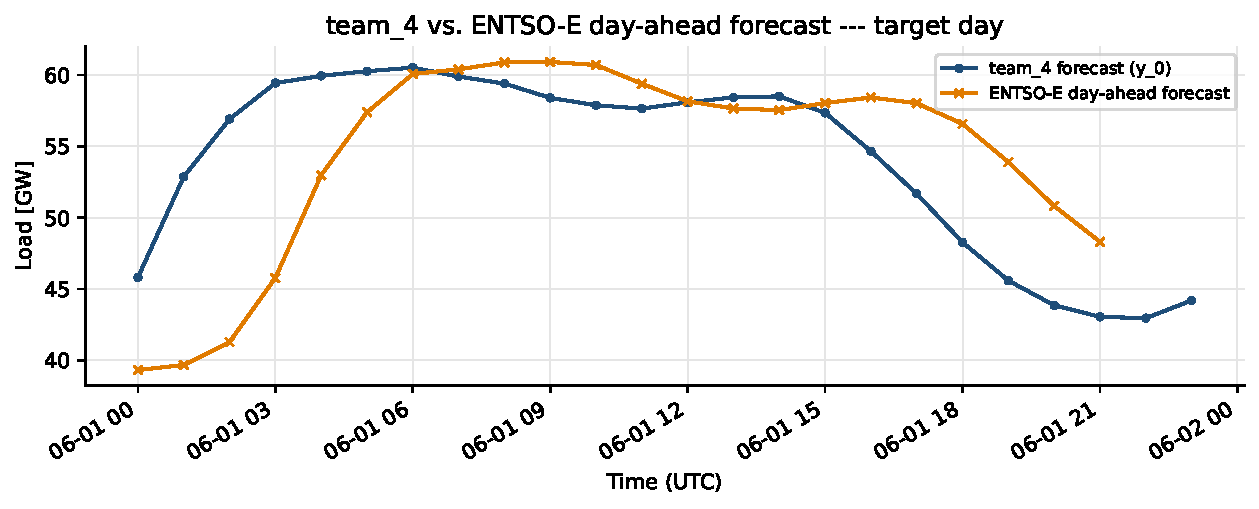
\includegraphics[keepaspectratio]{14_team_4_submission_files/figure-pdf/fig-team4-vs-entsoe-output-2.pdf}}

}

\caption{\label{fig-team4-vs-entsoe}ENTSO-E's published day-ahead
Forecasted Load for the target day (orange) vs.~team\_4's forecast
\texttt{y\_0} (blue), on the same 24 hourly steps. Neither is scored ---
the target day's actuals are not yet observed --- so this contrasts two
forecasts, not forecast against truth.}

\end{figure}%

\subsection{Validate the schema and write the submission
CSV}\label{sec-team4-write}

Same four contract assertions as Section~\ref{sec-live-example}: 24
rows, first stamp \texttt{TOMORROW\ 00:00\ UTC}, every value strictly
positive, no NaN. The write target is
\texttt{submissions/team\_4/\textless{}tomorrow\textgreater{}.csv}
inside the leaderboard fork.

\begin{Shaded}
\begin{Highlighting}[]
\ControlFlowTok{assert} \BuiltInTok{len}\NormalTok{(y0) }\OperatorTok{==} \DecValTok{24}\NormalTok{,           }\SpecialStringTok{f"expected 24 hourly steps for y\_0, got }\SpecialCharTok{\{}\BuiltInTok{len}\NormalTok{(y0)}\SpecialCharTok{\}}\SpecialStringTok{"}
\ControlFlowTok{assert}\NormalTok{ y0.index.}\BuiltInTok{min}\NormalTok{() }\OperatorTok{==}\NormalTok{ TOMORROW\_UTC, (}
    \SpecialStringTok{f"first step }\SpecialCharTok{\{}\NormalTok{y0}\SpecialCharTok{.}\NormalTok{index}\SpecialCharTok{.}\BuiltInTok{min}\NormalTok{()}\SpecialCharTok{\}}\SpecialStringTok{ != TOMORROW }\SpecialCharTok{\{}\NormalTok{TOMORROW\_UTC}\SpecialCharTok{\}}\SpecialStringTok{"}
\NormalTok{)}
\ControlFlowTok{assert}\NormalTok{ (y0 }\OperatorTok{\textgreater{}} \DecValTok{0}\NormalTok{).}\BuiltInTok{all}\NormalTok{(),          }\StringTok{"non{-}positive forecast value {-}{-}{-} spec requires \textgreater{} 0"}
\ControlFlowTok{assert}\NormalTok{ y0.notna().}\BuiltInTok{all}\NormalTok{(),        }\StringTok{"NaN in forecast {-}{-}{-} spec forbids"}

\NormalTok{TEAM\_ID }\OperatorTok{=} \StringTok{"team\_4"}
\NormalTok{SUBMISSION\_DIR }\OperatorTok{=}\NormalTok{ Path.home() }\OperatorTok{/} \StringTok{"workspace"} \OperatorTok{/} \StringTok{"challenge{-}leaderboard"} \OperatorTok{/} \StringTok{"submissions"} \OperatorTok{/}\NormalTok{ TEAM\_ID}
\NormalTok{SUBMISSION\_DIR.mkdir(parents}\OperatorTok{=}\VariableTok{True}\NormalTok{, exist\_ok}\OperatorTok{=}\VariableTok{True}\NormalTok{)}
\NormalTok{submission\_path }\OperatorTok{=}\NormalTok{ SUBMISSION\_DIR }\OperatorTok{/} \SpecialStringTok{f"}\SpecialCharTok{\{}\NormalTok{TOMORROW\_UTC}\SpecialCharTok{.}\NormalTok{date()}\SpecialCharTok{.}\NormalTok{isoformat()}\SpecialCharTok{\}}\SpecialStringTok{.csv"}

\NormalTok{submission\_df }\OperatorTok{=}\NormalTok{ pd.DataFrame(\{}
    \StringTok{"timestamp\_utc"}\NormalTok{: y0.index.strftime(}\StringTok{"\%Y{-}\%m{-}}\SpecialCharTok{\%d}\StringTok{T\%H:\%M:\%SZ"}\NormalTok{),}
    \StringTok{"forecast\_mw"}\NormalTok{:   y0.}\BuiltInTok{round}\NormalTok{(}\DecValTok{2}\NormalTok{).values,}
\NormalTok{\})}
\NormalTok{submission\_df.to\_csv(submission\_path, index}\OperatorTok{=}\VariableTok{False}\NormalTok{)}
\BuiltInTok{print}\NormalTok{(}\SpecialStringTok{f"wrote }\SpecialCharTok{\{}\NormalTok{submission\_path}\SpecialCharTok{\}}\SpecialStringTok{"}\NormalTok{)}
\BuiltInTok{print}\NormalTok{(}\SpecialStringTok{f"  rows: }\SpecialCharTok{\{}\BuiltInTok{len}\NormalTok{(submission\_df)}\SpecialCharTok{\}}\SpecialStringTok{"}\NormalTok{)}
\BuiltInTok{print}\NormalTok{(}\SpecialStringTok{f"  range: }\SpecialCharTok{\{}\NormalTok{submission\_df}\SpecialCharTok{.}\NormalTok{forecast\_mw}\SpecialCharTok{.}\BuiltInTok{min}\NormalTok{()}\SpecialCharTok{:.1f\}}\SpecialStringTok{–}\SpecialCharTok{\{}\NormalTok{submission\_df}\SpecialCharTok{.}\NormalTok{forecast\_mw}\SpecialCharTok{.}\BuiltInTok{max}\NormalTok{()}\SpecialCharTok{:.1f\}}\SpecialStringTok{ MW"}\NormalTok{)}
\NormalTok{submission\_df.head(}\DecValTok{3}\NormalTok{)}
\end{Highlighting}
\end{Shaded}

\begin{verbatim}
wrote /Users/bartz/workspace/challenge-leaderboard/submissions/team_4/2026-06-01.csv
  rows: 24
  range: 42959.2–60509.2 MW
\end{verbatim}

\protect\phantomsection\label{team4-submission-write}
{\def\LTcaptype{none} % do not increment counter
\begin{longtable}[]{@{}lll@{}}
\toprule\noalign{}
& timestamp\_utc & forecast\_mw \\
\midrule\noalign{}
\endhead
\bottomrule\noalign{}
\endlastfoot
0 & 2026-06-01T00:00:00Z & 45817.90 \\
1 & 2026-06-01T01:00:00Z & 52863.44 \\
2 & 2026-06-01T02:00:00Z & 56910.18 \\
\end{longtable}
}

\subsection{Local validation with the leaderboard's own
script}\label{local-validation-with-the-leaderboards-own-script-1}

\protect\phantomsection\label{team4-validate}
\begin{Shaded}
\begin{Highlighting}[]
\ImportTok{import}\NormalTok{ subprocess}
\NormalTok{lb\_repo }\OperatorTok{=}\NormalTok{ Path.home() }\OperatorTok{/} \StringTok{"workspace"} \OperatorTok{/} \StringTok{"challenge{-}leaderboard"}
\NormalTok{result }\OperatorTok{=}\NormalTok{ subprocess.run(}
\NormalTok{    [}
        \StringTok{"uv"}\NormalTok{, }\StringTok{"run"}\NormalTok{, }\StringTok{"python"}\NormalTok{, }\StringTok{"scripts/validate\_submission.py"}\NormalTok{,}
        \StringTok{"{-}{-}path"}\NormalTok{, }\BuiltInTok{str}\NormalTok{(submission\_path.relative\_to(lb\_repo)),}
        \StringTok{"{-}{-}skip{-}deadline"}\NormalTok{,}
\NormalTok{    ],}
\NormalTok{    cwd}\OperatorTok{=}\NormalTok{lb\_repo,}
\NormalTok{    capture\_output}\OperatorTok{=}\VariableTok{True}\NormalTok{,}
\NormalTok{    text}\OperatorTok{=}\VariableTok{True}\NormalTok{,}
\NormalTok{)}
\BuiltInTok{print}\NormalTok{(}\StringTok{"exit code:"}\NormalTok{, result.returncode)}
\BuiltInTok{print}\NormalTok{(}\StringTok{"stdout   :"}\NormalTok{, result.stdout.strip())}
\ControlFlowTok{if}\NormalTok{ result.stderr.strip():}
    \BuiltInTok{print}\NormalTok{(}\StringTok{"stderr   :"}\NormalTok{, result.stderr.strip())}
\end{Highlighting}
\end{Shaded}

\begin{verbatim}
exit code: 0
stdout   : OK: team=team_4 target_date=2026-06-01 file=submissions/team_4/2026-06-01.csv
\end{verbatim}

\section{Commit and push the submission PR}\label{sec-team4-push}

The cells above only \emph{write} the CSV --- they deliberately do not
commit, push, or open the PR (a careless render must not be able to spam
the leaderboard). Run the block below from a shell once the validation
cell above is green:

\begin{Shaded}
\begin{Highlighting}[]
\BuiltInTok{cd}\NormalTok{ \textasciitilde{}/workspace/challenge{-}leaderboard}
\CommentTok{\# TARGET=$(date {-}u {-}d \textquotesingle{}tomorrow\textquotesingle{} +\%F)                \# Linux equivalent}
\VariableTok{TARGET}\OperatorTok{=}\VariableTok{$(}\FunctionTok{date} \AttributeTok{{-}u} \AttributeTok{{-}v+1d}\NormalTok{ +\%F}\VariableTok{)}
\CommentTok{\# Unique branch per attempt: re{-}submitting for the same target day must not}
\CommentTok{\# collide with an earlier (already{-}merged) branch of the same name.}
\VariableTok{BRANCH}\OperatorTok{=}\StringTok{"submission/team\_4{-}}\VariableTok{$\{TARGET\}}\StringTok{{-}}\VariableTok{$(}\FunctionTok{date} \AttributeTok{{-}u}\NormalTok{ +\%H\%M\%S}\VariableTok{)}\StringTok{"}
\FunctionTok{git}\NormalTok{ switch }\AttributeTok{{-}c} \StringTok{"}\VariableTok{$BRANCH}\StringTok{"}\NormalTok{ main}
\FunctionTok{git}\NormalTok{ add }\StringTok{"submissions/team\_4/}\VariableTok{$\{TARGET\}}\StringTok{.csv"}
\FunctionTok{git}\NormalTok{ commit }\AttributeTok{{-}m} \StringTok{"submission(team\_4): forecast for }\VariableTok{$\{TARGET\}}\StringTok{"}
\FunctionTok{git}\NormalTok{ push }\AttributeTok{{-}u}\NormalTok{ origin }\StringTok{"}\VariableTok{$BRANCH}\StringTok{"}

\ExtensionTok{gh}\NormalTok{ pr create }\AttributeTok{{-}{-}base}\NormalTok{ main }\AttributeTok{{-}{-}repo}\NormalTok{ bartzbeielstein/challenge{-}leaderboard }\DataTypeTok{\textbackslash{}}
    \AttributeTok{{-}{-}head} \StringTok{"}\VariableTok{$BRANCH}\StringTok{"} \DataTypeTok{\textbackslash{}}
    \AttributeTok{{-}{-}title} \StringTok{"submission(team\_4): forecast for }\VariableTok{$\{TARGET\}}\StringTok{"} \DataTypeTok{\textbackslash{}}
    \AttributeTok{{-}{-}body}  \StringTok{"Generated by ddmo{-}sose{-}26 chapter 14 (team\_4 advanced submission)."}
\end{Highlighting}
\end{Shaded}

If validation on the PR passes, auto-merge squashes the submission onto
\texttt{main}. The next morning at 07:00 UTC the leaderboard's
\texttt{score-daily.yml} cron (see Section~\ref{sec-live-cron}) scores
it against ENTSO-E final actuals.

\begin{tcolorbox}[enhanced jigsaw, arc=.35mm, bottomrule=.15mm, bottomtitle=1mm, breakable, colback=white, colbacktitle=quarto-callout-warning-color!10!white, colframe=quarto-callout-warning-color-frame, coltitle=black, left=2mm, leftrule=.75mm, opacityback=0, opacitybacktitle=0.6, rightrule=.15mm, title=\textcolor{quarto-callout-warning-color}{\faExclamationTriangle}\hspace{0.5em}{Deadline}, titlerule=0mm, toprule=.15mm, toptitle=1mm]

Submissions for target day \texttt{D} must be merged before
\texttt{D-1\ 23:59\ UTC} --- the validator enforces this strictly. The
advanced configuration in this chapter renders in 5--10 minutes on a
typical laptop; give yourself at least 30 minutes of head-room before
the deadline.

\end{tcolorbox}

\section{What changed vs.~chapter 13 ---
summary}\label{sec-team4-summary}

{\def\LTcaptype{none} % do not increment counter
\begin{longtable}[]{@{}
  >{\raggedright\arraybackslash}p{(\linewidth - 4\tabcolsep) * \real{0.3333}}
  >{\raggedright\arraybackslash}p{(\linewidth - 4\tabcolsep) * \real{0.3333}}
  >{\raggedright\arraybackslash}p{(\linewidth - 4\tabcolsep) * \real{0.3333}}@{}}
\toprule\noalign{}
\begin{minipage}[b]{\linewidth}\raggedright
Knob
\end{minipage} & \begin{minipage}[b]{\linewidth}\raggedright
Chapter~\ref{sec-live-submission}
\end{minipage} & \begin{minipage}[b]{\linewidth}\raggedright
This chapter
\end{minipage} \\
\midrule\noalign{}
\endhead
\bottomrule\noalign{}
\endlastfoot
\texttt{periods} & \texttt{daily} only &
\texttt{daily,\ weekly,\ monthly,\ quarterly,\ yearly} \\
\texttt{lags\_consider} & \texttt{{[}1,\ 2,\ 24{]}} & data-selected via
PACF (1) \\
\texttt{warm\_start\_lags} & \texttt{False} (default) & \texttt{True} \\
\texttt{include\_weather\_windows} & (default) & \texttt{True} \\
\texttt{include\_holiday\_features} & (default) & \texttt{True} \\
\texttt{poly\_features\_degree} & \texttt{1} (off) & \texttt{2} \\
\texttt{max\_poly\_features} & \texttt{10} & \texttt{10} \\
\texttt{n\_trials\_spotoptim} & \texttt{10} & \texttt{6} \\
\texttt{n\_initial\_spotoptim} & \texttt{5} & \texttt{5} \\
\texttt{number\_folds} & \texttt{10} & \texttt{10} \\
Team id & \texttt{\textless{}team\_id\textgreater{}} placeholder &
\texttt{team\_4} (hardcoded) \\
\end{longtable}
}

\begin{tcolorbox}[enhanced jigsaw, arc=.35mm, bottomrule=.15mm, bottomtitle=1mm, breakable, colback=white, colbacktitle=quarto-callout-tip-color!10!white, colframe=quarto-callout-tip-color-frame, coltitle=black, left=2mm, leftrule=.75mm, opacityback=0, opacitybacktitle=0.6, rightrule=.15mm, title=\textcolor{quarto-callout-tip-color}{\faLightbulb}\hspace{0.5em}{Exercises (with Claude)}, titlerule=0mm, toprule=.15mm, toptitle=1mm]

\begin{enumerate}
\def\labelenumi{\arabic{enumi}.}
\tightlist
\item
  \emph{Did the bigger budget pay off?} Compare
  \texttt{metrics\_future\_one\_day} from this chapter against the same
  metric in Section~\ref{sec-live-example} for the same target day.
  Discuss with Claude whether the gain (or loss) justifies the extra
  \textasciitilde5 minutes of compute.
\item
  \emph{Ablate a feature.} Set \texttt{poly\_features\_degree=1}
  (interactions off) and re-render only the train + write cells. Does
  the MAE move noticeably? If not, the interactions are not load-bearing
  for this dataset.
\item
  \emph{Inspect the tuned hyperparameters.} Print
  \texttt{team4\_mt.results{[}"spotoptim"{]}{[}"Actual\ Load"{]}} keys
  and locate the best-trial summary. Which lag configuration did
  SpotOptim pick --- did the warm-started \texttt{key\_lags} win, or did
  a hardcoded candidate beat it?
\item
  \emph{How much does the CV block matter?} This chapter fixes the CV
  block at \texttt{cv\_block\_size=24}, decoupled from the live
  \texttt{predict\_size=LIVE\_N\_STEPS}
  (Section~\ref{sec-cross-validation-geometry}). Re-run the train cell
  with \texttt{cv\_block\_size=LIVE\_N\_STEPS} instead --- re-coupling
  the two --- and compare the tuned hyperparameters and
  \texttt{metrics\_future\_one\_day}, and watch the progress-bar total
  change from \texttt{70} to \texttt{⌈1680/LIVE\_N\_STEPS⌉}. Discuss
  with Claude why a recursive forecaster's CV score depends on the block
  length, and whether the fixed 24-hour block or the longer live horizon
  better matches the leaderboard's 24-hour metric.
\end{enumerate}

\end{tcolorbox}

\bookmarksetup{startatroot}

\chapter{ENTSO-E day-ahead baseline
submission}\label{sec-entsoe-submission}

\begin{tcolorbox}[enhanced jigsaw, arc=.35mm, bottomrule=.15mm, bottomtitle=1mm, breakable, colback=white, colbacktitle=quarto-callout-note-color!10!white, colframe=quarto-callout-note-color-frame, coltitle=black, left=2mm, leftrule=.75mm, opacityback=0, opacitybacktitle=0.6, rightrule=.15mm, title=\textcolor{quarto-callout-note-color}{\faInfo}\hspace{0.5em}{Learning objective}, titlerule=0mm, toprule=.15mm, toptitle=1mm]

You can submit the \emph{transmission system operators' own} 24-hour DE
load forecast --- ENTSO-E's published day-ahead
\texttt{Forecasted\ Load} --- as a zero-model baseline on the live
leaderboard, under the registered team \texttt{entsoe}. The chapter
shows why this baseline is the honest yardstick every tuned forecaster
in Chapter~\ref{sec-live-submission} and
Chapter~\ref{sec-team4-submission} must beat, and writes the validated
CSV into the leaderboard fork.

\end{tcolorbox}

\section{Overview}\label{sec-entsoe-overview}

Chapter~\ref{sec-live-submission} tunes an Optuna LightGBM forecaster;
Chapter~\ref{sec-team4-submission} tunes a richer SpotOptim variant.
Both pull ENTSO-E's own day-ahead \texttt{Forecasted\ Load} purely as a
comparison overlay (Section~\ref{sec-team4-vs-entsoe}) and never let the
model train on it. This chapter inverts that relationship: it submits
ENTSO-E's day-ahead forecast \emph{directly}, with no model at all.

That is deliberate. ENTSO-E aggregates the forecasts the European
transmission system operators already produce for grid scheduling, so it
is a strong, free, professionally-maintained baseline. A tuned model
that cannot beat it over the rolling 7-day window is not earning its
compute. Submitting it as its own team \texttt{entsoe} puts that
yardstick on the public leaderboard next to the student models, where
the comparison is unavoidable.

Every safety contract from Chapter~\ref{sec-live-submission} carries
over unchanged (24-row schema, strictly-positive forecasts, no NaN).
What disappears is the entire modelling stack: no \texttt{MultiTask}, no
\texttt{ConfigEntsoe}, no tuning, no exogenous features. The forecast is
a slice of the downloaded ENTSO-E frame. Two wrinkles specific to a
\emph{forward} baseline are handled along the way --- the safe
downloader drops future rows unless asked to keep them
(Section~\ref{sec-entsoe-query}), and a UTC target day straddles two
local publication days (Section~\ref{sec-entsoe-extract}).

\section{Submission contract}\label{submission-contract-1}

Unchanged --- see Section~\ref{sec-live-contract} for the CSV schema,
deadline, and scoring rules. The leaderboard validator that runs against
this chapter's output is byte-identical to the one used by
Chapter~\ref{sec-live-submission}. The only difference is the path:
\texttt{submissions/entsoe/\textless{}YYYY-MM-DD\textgreater{}.csv}.

\section{Team identity}\label{sec-entsoe-identity}

\texttt{entsoe} is hardcoded throughout this chapter --- there is no
placeholder to edit. The cell below confirms the team is registered in
\texttt{challenge-leaderboard/teams.yml}.

\protect\phantomsection\label{entsoe-registry}
\begin{Shaded}
\begin{Highlighting}[]
\ImportTok{from}\NormalTok{ pathlib }\ImportTok{import}\NormalTok{ Path}
\ImportTok{import}\NormalTok{ yaml}

\NormalTok{teams\_yml }\OperatorTok{=}\NormalTok{ Path.home() }\OperatorTok{/} \StringTok{"workspace"} \OperatorTok{/} \StringTok{"challenge{-}leaderboard"} \OperatorTok{/} \StringTok{"teams.yml"}
\NormalTok{teams }\OperatorTok{=}\NormalTok{ yaml.safe\_load(teams\_yml.read\_text())[}\StringTok{"teams"}\NormalTok{]}
\NormalTok{team }\OperatorTok{=} \BuiltInTok{next}\NormalTok{((t }\ControlFlowTok{for}\NormalTok{ t }\KeywordTok{in}\NormalTok{ teams }\ControlFlowTok{if}\NormalTok{ t[}\StringTok{"id"}\NormalTok{] }\OperatorTok{==} \StringTok{"entsoe"}\NormalTok{), }\VariableTok{None}\NormalTok{)}
\ControlFlowTok{assert}\NormalTok{ team }\KeywordTok{is} \KeywordTok{not} \VariableTok{None}\NormalTok{, }\StringTok{"entsoe is not in challenge{-}leaderboard/teams.yml"}
\BuiltInTok{print}\NormalTok{(}\SpecialStringTok{f"entsoe display\_name : }\SpecialCharTok{\{}\NormalTok{team[}\StringTok{\textquotesingle{}display\_name\textquotesingle{}}\NormalTok{]}\SpecialCharTok{\}}\SpecialStringTok{"}\NormalTok{)}
\BuiltInTok{print}\NormalTok{(}\SpecialStringTok{f"entsoe github       : }\SpecialCharTok{\{}\StringTok{\textquotesingle{}, \textquotesingle{}}\SpecialCharTok{.}\NormalTok{join(team[}\StringTok{\textquotesingle{}github\_handles\textquotesingle{}}\NormalTok{])}\SpecialCharTok{\}}\SpecialStringTok{"}\NormalTok{)}
\end{Highlighting}
\end{Shaded}

\begin{verbatim}
entsoe display_name : Entso-E
entsoe github       : bartzbeielstein
\end{verbatim}

\texttt{validate\_authorship()} in
\texttt{scripts/validate\_submission.py:89} rejects PRs whose author is
not in this \texttt{github\_handles} list, so the
\texttt{gh\ auth\ login} account used in Section~\ref{sec-entsoe-push}
must match.

\section{Prerequisites and
walkthrough}\label{prerequisites-and-walkthrough-1}

Identical to Section~\ref{sec-live-walkthrough}: Python 3.13 + uv, a
personal ENTSO-E API key exported as \texttt{ENTSOE\_API\_KEY},
\texttt{gh\ auth\ login} as a registered \texttt{entsoe} handle, and a
sibling clone of \texttt{challenge-leaderboard} at
\texttt{\textasciitilde{}/workspace/challenge-leaderboard/}. Because
there is no model to train, this chapter renders in seconds --- it
issues a single API call and slices it.

\section{Live pipeline}\label{sec-entsoe-example}

\protect\phantomsection\label{entsoe-imports}
\begin{Shaded}
\begin{Highlighting}[]
\ImportTok{import}\NormalTok{ os}
\ImportTok{from}\NormalTok{ pathlib }\ImportTok{import}\NormalTok{ Path}
\ImportTok{import}\NormalTok{ pandas }\ImportTok{as}\NormalTok{ pd}

\CommentTok{\# Isolate this chapter\textquotesingle{}s storage from chapters 13 and 14 (each pins its own}
\CommentTok{\# download home so the three chapters never read or write the same interim}
\CommentTok{\# file). The package reads the env var at call time via get\_data\_home().}
\NormalTok{os.environ[}\StringTok{"SPOTFORECAST2\_DATA"}\NormalTok{]  }\OperatorTok{=} \BuiltInTok{str}\NormalTok{(Path.home() }\OperatorTok{/} \StringTok{"spotforecast2\_data"}  \OperatorTok{/} \StringTok{"ddmo\_ch15\_entsoe"}\NormalTok{)}
\NormalTok{os.environ[}\StringTok{"SPOTFORECAST2\_CACHE"}\NormalTok{] }\OperatorTok{=} \BuiltInTok{str}\NormalTok{(Path.home() }\OperatorTok{/} \StringTok{".spotforecast2\_cache"} \OperatorTok{/} \StringTok{"ddmo\_ch15\_entsoe"}\NormalTok{)}

\ImportTok{from}\NormalTok{ spotforecast2\_safe.downloader.entsoe }\ImportTok{import}\NormalTok{ download\_new\_data}
\ImportTok{from}\NormalTok{ spotforecast2\_safe.data.fetch\_data }\ImportTok{import}\NormalTok{ get\_data\_home}

\NormalTok{api\_key }\OperatorTok{=}\NormalTok{ os.environ.get(}\StringTok{"ENTSOE\_API\_KEY"}\NormalTok{)}
\ControlFlowTok{assert}\NormalTok{ api\_key, }\StringTok{"ENTSOE\_API\_KEY must be set in the environment (see @sec{-}live{-}walkthrough Step 3)."}
\end{Highlighting}
\end{Shaded}

\subsection{Dynamic date constants}\label{dynamic-date-constants-2}

Every date is derived from
\texttt{pd.Timestamp.now(tz="UTC").normalize()} so the chapter stays
correct on every render --- same convention as
Section~\ref{sec-live-example}. \texttt{y\_0} is tomorrow's UTC day
(00:00--23:00 UTC), the 24 hourly stamps the leaderboard scores.

\protect\phantomsection\label{entsoe-constants}
\begin{Shaded}
\begin{Highlighting}[]
\NormalTok{NOW\_UTC }\OperatorTok{=}\NormalTok{ pd.Timestamp.now(tz}\OperatorTok{=}\StringTok{"UTC"}\NormalTok{)}
\NormalTok{TODAY\_UTC }\OperatorTok{=}\NormalTok{ NOW\_UTC.normalize()}
\NormalTok{TOMORROW\_UTC }\OperatorTok{=}\NormalTok{ TODAY\_UTC }\OperatorTok{+}\NormalTok{ pd.Timedelta(days}\OperatorTok{=}\DecValTok{1}\NormalTok{)}
\NormalTok{LAST\_TARGET }\OperatorTok{=}\NormalTok{ TOMORROW\_UTC }\OperatorTok{+}\NormalTok{ pd.Timedelta(hours}\OperatorTok{=}\DecValTok{23}\NormalTok{)}

\CommentTok{\# A day{-}ahead baseline needs no training history {-}{-}{-} only a short recent window:}
\CommentTok{\# enough to carry the last week of \textasciigrave{}Actual Load\textasciigrave{} for the context plot plus a}
\CommentTok{\# previous{-}day fallback (@sec{-}entsoe{-}extract). We download the last 10 days and}
\CommentTok{\# reach the end through the day *after* tomorrow so the full target day is}
\CommentTok{\# covered as soon as ENTSO{-}E publishes it. download\_new\_data takes the window as}
\CommentTok{\# \textquotesingle{}YYYYMMDDHH00\textquotesingle{} strings.}
\NormalTok{START\_DOWNLOAD }\OperatorTok{=}\NormalTok{ (TODAY\_UTC }\OperatorTok{{-}}\NormalTok{ pd.Timedelta(days}\OperatorTok{=}\DecValTok{10}\NormalTok{)).strftime(}\StringTok{"\%Y\%m}\SpecialCharTok{\%d}\StringTok{\%H\%M"}\NormalTok{)}
\NormalTok{END\_DOWNLOAD }\OperatorTok{=}\NormalTok{ (TOMORROW\_UTC }\OperatorTok{+}\NormalTok{ pd.Timedelta(days}\OperatorTok{=}\DecValTok{1}\NormalTok{)).strftime(}\StringTok{"\%Y\%m}\SpecialCharTok{\%d}\StringTok{\%H\%M"}\NormalTok{)}

\BuiltInTok{print}\NormalTok{(}\SpecialStringTok{f"NOW\_UTC        = }\SpecialCharTok{\{}\NormalTok{NOW\_UTC}\SpecialCharTok{\}}\SpecialStringTok{"}\NormalTok{)}
\BuiltInTok{print}\NormalTok{(}\SpecialStringTok{f"TODAY\_UTC      = }\SpecialCharTok{\{}\NormalTok{TODAY\_UTC}\SpecialCharTok{\}}\SpecialStringTok{"}\NormalTok{)}
\BuiltInTok{print}\NormalTok{(}\SpecialStringTok{f"TOMORROW\_UTC   = }\SpecialCharTok{\{}\NormalTok{TOMORROW\_UTC}\SpecialCharTok{\}}\SpecialStringTok{  (target day = y\_0)"}\NormalTok{)}
\BuiltInTok{print}\NormalTok{(}\SpecialStringTok{f"LAST\_TARGET    = }\SpecialCharTok{\{}\NormalTok{LAST\_TARGET}\SpecialCharTok{\}}\SpecialStringTok{"}\NormalTok{)}
\BuiltInTok{print}\NormalTok{(}\SpecialStringTok{f"START\_DOWNLOAD = }\SpecialCharTok{\{}\NormalTok{START\_DOWNLOAD}\SpecialCharTok{\}}\SpecialStringTok{  (10 days back {-}{-}{-} no training history)"}\NormalTok{)}
\BuiltInTok{print}\NormalTok{(}\SpecialStringTok{f"END\_DOWNLOAD   = }\SpecialCharTok{\{}\NormalTok{END\_DOWNLOAD}\SpecialCharTok{\}}\SpecialStringTok{  (covers tomorrow\textquotesingle{}s day{-}ahead forecast)"}\NormalTok{)}
\end{Highlighting}
\end{Shaded}

\begin{verbatim}
NOW_UTC        = 2026-05-31 20:20:24.505450+00:00
TODAY_UTC      = 2026-05-31 00:00:00+00:00
TOMORROW_UTC   = 2026-06-01 00:00:00+00:00  (target day = y_0)
LAST_TARGET    = 2026-06-01 23:00:00+00:00
START_DOWNLOAD = 202605210000  (10 days back --- no training history)
END_DOWNLOAD   = 202606020000  (covers tomorrow's day-ahead forecast)
\end{verbatim}

\subsection{\texorpdfstring{Download ENTSO-E's day-ahead
\texttt{Forecasted\ Load}}{Download ENTSO-E's day-ahead Forecasted Load}}\label{sec-entsoe-query}

We fetch through the same safe wrapper the training chapters use,
\texttt{spotforecast2\_safe.downloader.entsoe.download\_new\_data}, with
one argument that matters here: \texttt{keep\_forecast\_future=True}. By
default the wrapper drops every row after \texttt{now} when it merges
the download into the interim file ---

\begin{Shaded}
\begin{Highlighting}[]
\CommentTok{\# spotforecast2\_safe/downloader/entsoe.py}
\ControlFlowTok{if} \KeywordTok{not}\NormalTok{ keep\_forecast\_future:}
\NormalTok{    merged\_df }\OperatorTok{=}\NormalTok{ merged\_df.loc[merged\_df.index }\OperatorTok{\textless{}=}\NormalTok{ pd.Timestamp.now(tz}\OperatorTok{=}\StringTok{"UTC"}\NormalTok{)]}
\end{Highlighting}
\end{Shaded}

That truncation is correct for the training chapters (a model must never
see the future), but it would erase the very thing this baseline
submits: ENTSO-E's day-ahead \texttt{Forecasted\ Load} for tomorrow. The
flag keeps those future rows; future \texttt{Actual\ Load} is still
blank, so nothing leaks --- there is no model here in any case.
ENTSO-E's \texttt{Forecasted\ Load} is published per \emph{local}
(Europe/Berlin) day; the wrapper normalises the merged interim index to
UTC, the zone the leaderboard scores in.

\protect\phantomsection\label{entsoe-query}
\begin{Shaded}
\begin{Highlighting}[]
\NormalTok{download\_new\_data(}
\NormalTok{    api\_key}\OperatorTok{=}\NormalTok{api\_key,}
\NormalTok{    country\_code}\OperatorTok{=}\StringTok{"DE"}\NormalTok{,}
\NormalTok{    start}\OperatorTok{=}\NormalTok{START\_DOWNLOAD,}
\NormalTok{    end}\OperatorTok{=}\NormalTok{END\_DOWNLOAD,}
\NormalTok{    force}\OperatorTok{=}\VariableTok{True}\NormalTok{,}
\NormalTok{    keep\_forecast\_future}\OperatorTok{=}\VariableTok{True}\NormalTok{,   }\CommentTok{\# keep tomorrow\textquotesingle{}s day{-}ahead forecast}
\NormalTok{)}

\NormalTok{interim\_csv }\OperatorTok{=}\NormalTok{ get\_data\_home() }\OperatorTok{/} \StringTok{"interim"} \OperatorTok{/} \StringTok{"energy\_load.csv"}
\NormalTok{interim }\OperatorTok{=}\NormalTok{ pd.read\_csv(interim\_csv, index\_col}\OperatorTok{=}\DecValTok{0}\NormalTok{, parse\_dates}\OperatorTok{=}\VariableTok{True}\NormalTok{)}
\NormalTok{interim.index }\OperatorTok{=}\NormalTok{ pd.to\_datetime(interim.index, utc}\OperatorTok{=}\VariableTok{True}\NormalTok{)}

\BuiltInTok{print}\NormalTok{(}\SpecialStringTok{f"interim rows       : }\SpecialCharTok{\{}\BuiltInTok{len}\NormalTok{(interim)}\SpecialCharTok{\}}\SpecialStringTok{ (15{-}min, }\SpecialCharTok{\{}\NormalTok{interim}\SpecialCharTok{.}\NormalTok{index}\SpecialCharTok{.}\BuiltInTok{min}\NormalTok{()}\SpecialCharTok{\}}\SpecialStringTok{ → }\SpecialCharTok{\{}\NormalTok{interim}\SpecialCharTok{.}\NormalTok{index}\SpecialCharTok{.}\BuiltInTok{max}\NormalTok{()}\SpecialCharTok{\}}\SpecialStringTok{)"}\NormalTok{)}
\BuiltInTok{print}\NormalTok{(}\SpecialStringTok{f"columns            : }\SpecialCharTok{\{}\BuiltInTok{list}\NormalTok{(interim.columns)}\SpecialCharTok{\}}\SpecialStringTok{"}\NormalTok{)}
\BuiltInTok{print}\NormalTok{(}\SpecialStringTok{f"Forecasted Load to : }\SpecialCharTok{\{}\NormalTok{interim[}\StringTok{\textquotesingle{}Forecasted Load\textquotesingle{}}\NormalTok{]}\SpecialCharTok{.}\NormalTok{dropna()}\SpecialCharTok{.}\NormalTok{index}\SpecialCharTok{.}\BuiltInTok{max}\NormalTok{()}\SpecialCharTok{\}}\SpecialStringTok{"}\NormalTok{)}
\BuiltInTok{print}\NormalTok{(}\SpecialStringTok{f"Actual Load to     : }\SpecialCharTok{\{}\NormalTok{interim[}\StringTok{\textquotesingle{}Actual Load\textquotesingle{}}\NormalTok{]}\SpecialCharTok{.}\NormalTok{dropna()}\SpecialCharTok{.}\NormalTok{index}\SpecialCharTok{.}\BuiltInTok{max}\NormalTok{()}\SpecialCharTok{\}}\SpecialStringTok{"}\NormalTok{)}
\end{Highlighting}
\end{Shaded}

\begin{verbatim}
interim rows       : 1144 (15-min, 2026-05-21 00:00:00+00:00 → 2026-06-01 21:45:00+00:00)
columns            : ['Forecasted Load', 'Actual Load']
Forecasted Load to : 2026-06-01 21:45:00+00:00
Actual Load to     : 2026-05-31 19:15:00+00:00
\end{verbatim}

We aggregate the 15-minute series onto the hourly grid the leaderboard
scores on --- the mean of each hour's four quarter-hour values, matching
how the tuned chapters aggregate the actuals.

\protect\phantomsection\label{entsoe-hourly}
\begin{Shaded}
\begin{Highlighting}[]
\NormalTok{forecast\_h }\OperatorTok{=}\NormalTok{ interim[}\StringTok{"Forecasted Load"}\NormalTok{].resample(}\StringTok{"h"}\NormalTok{).mean().dropna()}
\NormalTok{actual\_h }\OperatorTok{=}\NormalTok{ interim[}\StringTok{"Actual Load"}\NormalTok{].resample(}\StringTok{"h"}\NormalTok{).mean().dropna()}
\NormalTok{forecast\_h.name }\OperatorTok{=} \StringTok{"Forecasted Load"}
\NormalTok{actual\_h.name }\OperatorTok{=} \StringTok{"Actual Load"}

\BuiltInTok{print}\NormalTok{(}\SpecialStringTok{f"hourly forecast : }\SpecialCharTok{\{}\BuiltInTok{len}\NormalTok{(forecast\_h)}\SpecialCharTok{\}}\SpecialStringTok{ h | }\SpecialCharTok{\{}\NormalTok{forecast\_h}\SpecialCharTok{.}\NormalTok{index}\SpecialCharTok{.}\BuiltInTok{min}\NormalTok{()}\SpecialCharTok{\}}\SpecialStringTok{ → }\SpecialCharTok{\{}\NormalTok{forecast\_h}\SpecialCharTok{.}\NormalTok{index}\SpecialCharTok{.}\BuiltInTok{max}\NormalTok{()}\SpecialCharTok{\}}\SpecialStringTok{"}\NormalTok{)}
\BuiltInTok{print}\NormalTok{(}\SpecialStringTok{f"hourly actual   : }\SpecialCharTok{\{}\BuiltInTok{len}\NormalTok{(actual\_h)}\SpecialCharTok{\}}\SpecialStringTok{ h | }\SpecialCharTok{\{}\NormalTok{actual\_h}\SpecialCharTok{.}\NormalTok{index}\SpecialCharTok{.}\BuiltInTok{min}\NormalTok{()}\SpecialCharTok{\}}\SpecialStringTok{ → }\SpecialCharTok{\{}\NormalTok{actual\_h}\SpecialCharTok{.}\NormalTok{index}\SpecialCharTok{.}\BuiltInTok{max}\NormalTok{()}\SpecialCharTok{\}}\SpecialStringTok{"}\NormalTok{)}
\end{Highlighting}
\end{Shaded}

\begin{verbatim}
hourly forecast : 286 h | 2026-05-21 00:00:00+00:00 → 2026-06-01 21:00:00+00:00
hourly actual   : 260 h | 2026-05-21 00:00:00+00:00 → 2026-05-31 19:00:00+00:00
\end{verbatim}

\subsection{Assemble the 24-hour target slice}\label{sec-entsoe-extract}

The target is the 24 UTC hours of tomorrow, \texttt{00:00\ …\ 23:00}.
ENTSO-E publishes its day-ahead forecast per \emph{local}
(Europe/Berlin) day, and Germany runs one or two hours ahead of UTC. So
at submission time --- the afternoon of \texttt{D-1}, when only the
local \texttt{D} day-ahead is out --- the last one or two UTC hours of
the target (\texttt{22:00}, \texttt{23:00} UTC) fall into the
\emph{next} local day, which ENTSO-E does not publish until \texttt{D},
after the \texttt{D-1\ 23:59\ UTC} deadline.

Those trailing hours are therefore filled with ENTSO-E's own forecast
for the same clock hour 24 hours earlier --- a transparent, fully
reproducible persistence of the operators' published forecast (today's
day-ahead is already complete, so the fallback source always exists).
The fill is logged, and a fail-loud guard (CR-3) aborts if even the
fallback is missing rather than writing a short or NaN-padded CSV.

\protect\phantomsection\label{entsoe-extract}
\begin{Shaded}
\begin{Highlighting}[]
\NormalTok{target\_index }\OperatorTok{=}\NormalTok{ pd.date\_range(TOMORROW\_UTC, LAST\_TARGET, freq}\OperatorTok{=}\StringTok{"h"}\NormalTok{, tz}\OperatorTok{=}\StringTok{"UTC"}\NormalTok{)  }\CommentTok{\# 24 stamps}
\NormalTok{y0 }\OperatorTok{=}\NormalTok{ forecast\_h.reindex(target\_index)}

\NormalTok{published }\OperatorTok{=} \BuiltInTok{int}\NormalTok{(y0.notna().}\BuiltInTok{sum}\NormalTok{())}
\NormalTok{missing }\OperatorTok{=}\NormalTok{ y0.index[y0.isna()]}
\BuiltInTok{print}\NormalTok{(}\SpecialStringTok{f"day{-}ahead hours published for }\SpecialCharTok{\{}\NormalTok{TOMORROW\_UTC}\SpecialCharTok{.}\NormalTok{date()}\SpecialCharTok{\}}\SpecialStringTok{: }\SpecialCharTok{\{}\NormalTok{published}\SpecialCharTok{\}}\SpecialStringTok{ / 24"}\NormalTok{)}

\ControlFlowTok{for}\NormalTok{ ts }\KeywordTok{in}\NormalTok{ missing:}
\NormalTok{    fallback }\OperatorTok{=}\NormalTok{ forecast\_h.reindex([ts }\OperatorTok{{-}}\NormalTok{ pd.Timedelta(days}\OperatorTok{=}\DecValTok{1}\NormalTok{)]).iloc[}\DecValTok{0}\NormalTok{]}
    \ControlFlowTok{if}\NormalTok{ pd.isna(fallback):}
        \ControlFlowTok{raise} \PreprocessorTok{RuntimeError}\NormalTok{(}
            \SpecialStringTok{f"No day{-}ahead value for }\SpecialCharTok{\{}\NormalTok{ts}\SpecialCharTok{\}}\SpecialStringTok{ and no 24 h{-}earlier fallback either; "}
            \StringTok{"ENTSO{-}E coverage is too thin to assemble 24 hours. Re{-}render once "}
            \StringTok{"the day{-}ahead forecast for the target day is published."}
\NormalTok{        )}
\NormalTok{    y0.loc[ts] }\OperatorTok{=}\NormalTok{ fallback}
    \BuiltInTok{print}\NormalTok{(}\SpecialStringTok{f"  filled }\SpecialCharTok{\{}\NormalTok{ts}\SpecialCharTok{\}}\SpecialStringTok{ ← }\SpecialCharTok{\{}\NormalTok{ts }\OperatorTok{{-}}\NormalTok{ pd}\SpecialCharTok{.}\NormalTok{Timedelta(days}\OperatorTok{=}\DecValTok{1}\NormalTok{)}\SpecialCharTok{\}}\SpecialStringTok{ (24 h{-}earlier ENTSO{-}E forecast = }\SpecialCharTok{\{}\NormalTok{fallback}\SpecialCharTok{:,.0f\}}\SpecialStringTok{ MW)"}\NormalTok{)}

\NormalTok{y0.name }\OperatorTok{=} \StringTok{"Forecasted Load"}
\BuiltInTok{print}\NormalTok{(}\SpecialStringTok{f"}\CharTok{\textbackslash{}n}\SpecialStringTok{y\_0 assembled: }\SpecialCharTok{\{}\BuiltInTok{len}\NormalTok{(y0)}\SpecialCharTok{\}}\SpecialStringTok{ hourly steps | }\SpecialCharTok{\{}\NormalTok{y0}\SpecialCharTok{.}\NormalTok{index}\SpecialCharTok{.}\BuiltInTok{min}\NormalTok{()}\SpecialCharTok{\}}\SpecialStringTok{ → }\SpecialCharTok{\{}\NormalTok{y0}\SpecialCharTok{.}\NormalTok{index}\SpecialCharTok{.}\BuiltInTok{max}\NormalTok{()}\SpecialCharTok{\}}\SpecialStringTok{"}\NormalTok{)}
\BuiltInTok{print}\NormalTok{(y0)}
\end{Highlighting}
\end{Shaded}

\begin{verbatim}
day-ahead hours published for 2026-06-01: 22 / 24
  filled 2026-06-01 22:00:00+00:00 ← 2026-05-31 22:00:00+00:00 (24 h-earlier ENTSO-E forecast = 41,048 MW)
  filled 2026-06-01 23:00:00+00:00 ← 2026-05-31 23:00:00+00:00 (24 h-earlier ENTSO-E forecast = 39,752 MW)

y_0 assembled: 24 hourly steps | 2026-06-01 00:00:00+00:00 → 2026-06-01 23:00:00+00:00
2026-06-01 00:00:00+00:00    39327.047789
2026-06-01 01:00:00+00:00    39675.580085
2026-06-01 02:00:00+00:00    41285.199476
2026-06-01 03:00:00+00:00    45776.233649
2026-06-01 04:00:00+00:00    52975.273053
2026-06-01 05:00:00+00:00    57379.896787
2026-06-01 06:00:00+00:00    60062.325011
2026-06-01 07:00:00+00:00    60396.462782
2026-06-01 08:00:00+00:00    60874.850613
2026-06-01 09:00:00+00:00    60911.805267
2026-06-01 10:00:00+00:00    60694.146027
2026-06-01 11:00:00+00:00    59381.019278
2026-06-01 12:00:00+00:00    58150.097945
2026-06-01 13:00:00+00:00    57647.152979
2026-06-01 14:00:00+00:00    57535.920035
2026-06-01 15:00:00+00:00    58022.758576
2026-06-01 16:00:00+00:00    58422.032589
2026-06-01 17:00:00+00:00    58017.811127
2026-06-01 18:00:00+00:00    56567.745495
2026-06-01 19:00:00+00:00    53892.870363
2026-06-01 20:00:00+00:00    50815.118195
2026-06-01 21:00:00+00:00    48307.254943
2026-06-01 22:00:00+00:00    41047.617584
2026-06-01 23:00:00+00:00    39752.114576
Freq: h, Name: Forecasted Load, dtype: float64
\end{verbatim}

\subsection{Visual inspection}\label{visual-inspection-2}

The plot overlays the last week of published \texttt{Actual\ Load}
(blue) with ENTSO-E's day-ahead \texttt{Forecasted\ Load} running into
the target day (orange). The 24 hourly values we submit are the shaded
block; any fallback-filled trailing hours are marked.

\begin{Shaded}
\begin{Highlighting}[]
\ImportTok{import}\NormalTok{ matplotlib.pyplot }\ImportTok{as}\NormalTok{ plt}

\NormalTok{LAST\_WEEK\_START }\OperatorTok{=}\NormalTok{ TODAY\_UTC }\OperatorTok{{-}}\NormalTok{ pd.Timedelta(days}\OperatorTok{=}\DecValTok{7}\NormalTok{)}
\NormalTok{actual\_view }\OperatorTok{=}\NormalTok{ actual\_h.loc[LAST\_WEEK\_START:]}
\NormalTok{fc\_view }\OperatorTok{=}\NormalTok{ forecast\_h.loc[LAST\_WEEK\_START:]}
\NormalTok{filled }\OperatorTok{=}\NormalTok{ y0.index[}\OperatorTok{\textasciitilde{}}\NormalTok{y0.index.isin(forecast\_h.index)]}

\NormalTok{fig, ax }\OperatorTok{=}\NormalTok{ plt.subplots(figsize}\OperatorTok{=}\NormalTok{(}\FloatTok{8.5}\NormalTok{, }\FloatTok{3.5}\NormalTok{))}
\NormalTok{ax.plot(actual\_view.index, actual\_view.values }\OperatorTok{/} \DecValTok{1000}\NormalTok{, color}\OperatorTok{=}\StringTok{"\#1F4E79"}\NormalTok{,}
\NormalTok{        lw}\OperatorTok{=}\FloatTok{1.2}\NormalTok{, label}\OperatorTok{=}\StringTok{"Actual Load (published)"}\NormalTok{)}
\NormalTok{ax.plot(fc\_view.index, fc\_view.values }\OperatorTok{/} \DecValTok{1000}\NormalTok{, color}\OperatorTok{=}\StringTok{"\#E07B00"}\NormalTok{,}
\NormalTok{        lw}\OperatorTok{=}\FloatTok{1.2}\NormalTok{, label}\OperatorTok{=}\StringTok{"ENTSO{-}E day{-}ahead forecast"}\NormalTok{)}
\NormalTok{ax.plot(y0.index, y0.values }\OperatorTok{/} \DecValTok{1000}\NormalTok{, color}\OperatorTok{=}\StringTok{"\#E07B00"}\NormalTok{, lw}\OperatorTok{=}\DecValTok{0}\NormalTok{, marker}\OperatorTok{=}\StringTok{"o"}\NormalTok{, ms}\OperatorTok{=}\DecValTok{3}\NormalTok{)}
\ControlFlowTok{if} \BuiltInTok{len}\NormalTok{(filled):}
\NormalTok{    ax.plot(filled, y0.loc[filled].values }\OperatorTok{/} \DecValTok{1000}\NormalTok{, color}\OperatorTok{=}\StringTok{"\#B22222"}\NormalTok{, lw}\OperatorTok{=}\DecValTok{0}\NormalTok{,}
\NormalTok{            marker}\OperatorTok{=}\StringTok{"x"}\NormalTok{, ms}\OperatorTok{=}\DecValTok{7}\NormalTok{, label}\OperatorTok{=}\StringTok{"fallback (24 h{-}earlier forecast)"}\NormalTok{)}
\NormalTok{ax.axvspan(TOMORROW\_UTC, LAST\_TARGET, color}\OperatorTok{=}\StringTok{"\#E07B00"}\NormalTok{, alpha}\OperatorTok{=}\FloatTok{0.10}\NormalTok{,}
\NormalTok{           label}\OperatorTok{=}\StringTok{"target day (y\_0)"}\NormalTok{)}
\NormalTok{ax.set\_xlabel(}\StringTok{"Time (UTC)"}\NormalTok{)}
\NormalTok{ax.set\_ylabel(}\StringTok{"Load [GW]"}\NormalTok{)}
\NormalTok{ax.set\_title(}\StringTok{"ENTSO{-}E DE day{-}ahead baseline {-}{-}{-} last week + target day"}\NormalTok{)}
\NormalTok{ax.grid(}\VariableTok{True}\NormalTok{, color}\OperatorTok{=}\StringTok{"\#E5E5E5"}\NormalTok{, linewidth}\OperatorTok{=}\FloatTok{0.5}\NormalTok{)}
\NormalTok{ax.legend(fontsize}\OperatorTok{=}\DecValTok{8}\NormalTok{)}
\ControlFlowTok{for}\NormalTok{ s }\KeywordTok{in}\NormalTok{ (}\StringTok{"top"}\NormalTok{, }\StringTok{"right"}\NormalTok{):}
\NormalTok{    ax.spines[s].set\_visible(}\VariableTok{False}\NormalTok{)}
\NormalTok{fig.autofmt\_xdate()}
\NormalTok{fig.tight\_layout()}
\NormalTok{plt.show()}
\end{Highlighting}
\end{Shaded}

\begin{figure}[H]

\centering{

\pandocbounded{\includegraphics[keepaspectratio]{15_entsoe_files/figure-pdf/fig-entsoe-forecast-output-1.pdf}}

}

\caption{\label{fig-entsoe-forecast}ENTSO-E DE day-ahead baseline. Blue:
the last week of published \texttt{Actual\ Load}. Orange: ENTSO-E's
day-ahead \texttt{Forecasted\ Load}. The 24 hourly values for
\texttt{y\_0} (shaded) are exactly the CSV we submit; red crosses mark
any trailing UTC hour filled from the 24 h-earlier forecast
(Section~\ref{sec-entsoe-extract}).}

\end{figure}%

\subsection{Validate the schema and write the submission
CSV}\label{sec-entsoe-write}

The same four contract assertions as Section~\ref{sec-live-example}
guard the write: 24 rows, the first stamp must be
\texttt{TOMORROW\ 00:00\ UTC}, every value strictly positive, no NaN.
Any violation aborts before the file is opened, so a partially-written
CSV can never reach the leaderboard.

\begin{Shaded}
\begin{Highlighting}[]
\ControlFlowTok{assert} \BuiltInTok{len}\NormalTok{(y0) }\OperatorTok{==} \DecValTok{24}\NormalTok{,           }\SpecialStringTok{f"expected 24 hourly steps for y\_0, got }\SpecialCharTok{\{}\BuiltInTok{len}\NormalTok{(y0)}\SpecialCharTok{\}}\SpecialStringTok{"}
\ControlFlowTok{assert}\NormalTok{ y0.index.}\BuiltInTok{min}\NormalTok{() }\OperatorTok{==}\NormalTok{ TOMORROW\_UTC, (}
    \SpecialStringTok{f"first step }\SpecialCharTok{\{}\NormalTok{y0}\SpecialCharTok{.}\NormalTok{index}\SpecialCharTok{.}\BuiltInTok{min}\NormalTok{()}\SpecialCharTok{\}}\SpecialStringTok{ != TOMORROW }\SpecialCharTok{\{}\NormalTok{TOMORROW\_UTC}\SpecialCharTok{\}}\SpecialStringTok{"}
\NormalTok{)}
\ControlFlowTok{assert}\NormalTok{ (y0 }\OperatorTok{\textgreater{}} \DecValTok{0}\NormalTok{).}\BuiltInTok{all}\NormalTok{(),          }\StringTok{"non{-}positive forecast value {-}{-}{-} spec requires \textgreater{} 0"}
\ControlFlowTok{assert}\NormalTok{ y0.notna().}\BuiltInTok{all}\NormalTok{(),        }\StringTok{"NaN in forecast {-}{-}{-} spec forbids"}

\NormalTok{TEAM\_ID }\OperatorTok{=} \StringTok{"entsoe"}
\NormalTok{SUBMISSION\_DIR }\OperatorTok{=}\NormalTok{ Path.home() }\OperatorTok{/} \StringTok{"workspace"} \OperatorTok{/} \StringTok{"challenge{-}leaderboard"} \OperatorTok{/} \StringTok{"submissions"} \OperatorTok{/}\NormalTok{ TEAM\_ID}
\NormalTok{SUBMISSION\_DIR.mkdir(parents}\OperatorTok{=}\VariableTok{True}\NormalTok{, exist\_ok}\OperatorTok{=}\VariableTok{True}\NormalTok{)}
\NormalTok{submission\_path }\OperatorTok{=}\NormalTok{ SUBMISSION\_DIR }\OperatorTok{/} \SpecialStringTok{f"}\SpecialCharTok{\{}\NormalTok{TOMORROW\_UTC}\SpecialCharTok{.}\NormalTok{date()}\SpecialCharTok{.}\NormalTok{isoformat()}\SpecialCharTok{\}}\SpecialStringTok{.csv"}

\NormalTok{submission\_df }\OperatorTok{=}\NormalTok{ pd.DataFrame(\{}
    \StringTok{"timestamp\_utc"}\NormalTok{: y0.index.strftime(}\StringTok{"\%Y{-}\%m{-}}\SpecialCharTok{\%d}\StringTok{T\%H:\%M:\%SZ"}\NormalTok{),}
    \StringTok{"forecast\_mw"}\NormalTok{:   y0.}\BuiltInTok{round}\NormalTok{(}\DecValTok{2}\NormalTok{).values,}
\NormalTok{\})}
\NormalTok{submission\_df.to\_csv(submission\_path, index}\OperatorTok{=}\VariableTok{False}\NormalTok{)}
\BuiltInTok{print}\NormalTok{(}\SpecialStringTok{f"wrote }\SpecialCharTok{\{}\NormalTok{submission\_path}\SpecialCharTok{\}}\SpecialStringTok{"}\NormalTok{)}
\BuiltInTok{print}\NormalTok{(}\SpecialStringTok{f"  rows: }\SpecialCharTok{\{}\BuiltInTok{len}\NormalTok{(submission\_df)}\SpecialCharTok{\}}\SpecialStringTok{"}\NormalTok{)}
\BuiltInTok{print}\NormalTok{(}\SpecialStringTok{f"  range: }\SpecialCharTok{\{}\NormalTok{submission\_df}\SpecialCharTok{.}\NormalTok{forecast\_mw}\SpecialCharTok{.}\BuiltInTok{min}\NormalTok{()}\SpecialCharTok{:.1f\}}\SpecialStringTok{–}\SpecialCharTok{\{}\NormalTok{submission\_df}\SpecialCharTok{.}\NormalTok{forecast\_mw}\SpecialCharTok{.}\BuiltInTok{max}\NormalTok{()}\SpecialCharTok{:.1f\}}\SpecialStringTok{ MW"}\NormalTok{)}
\NormalTok{submission\_df.head(}\DecValTok{3}\NormalTok{)}
\end{Highlighting}
\end{Shaded}

\begin{verbatim}
wrote /Users/bartz/workspace/challenge-leaderboard/submissions/entsoe/2026-06-01.csv
  rows: 24
  range: 39327.1–60911.8 MW
\end{verbatim}

\protect\phantomsection\label{entsoe-submission-write}
{\def\LTcaptype{none} % do not increment counter
\begin{longtable}[]{@{}lll@{}}
\toprule\noalign{}
& timestamp\_utc & forecast\_mw \\
\midrule\noalign{}
\endhead
\bottomrule\noalign{}
\endlastfoot
0 & 2026-06-01T00:00:00Z & 39327.05 \\
1 & 2026-06-01T01:00:00Z & 39675.58 \\
2 & 2026-06-01T02:00:00Z & 41285.20 \\
\end{longtable}
}

\subsection{Local validation with the leaderboard's own
script}\label{local-validation-with-the-leaderboards-own-script-2}

A green exit code from \texttt{validate\_submission.py} is the same
check that runs on the PR in CI. We pass \texttt{-\/-skip-deadline}
because the chapter may be rendered inside the deadline window (the live
CI uses the strict form without the flag).

\protect\phantomsection\label{entsoe-validate}
\begin{Shaded}
\begin{Highlighting}[]
\ImportTok{import}\NormalTok{ subprocess}
\NormalTok{lb\_repo }\OperatorTok{=}\NormalTok{ Path.home() }\OperatorTok{/} \StringTok{"workspace"} \OperatorTok{/} \StringTok{"challenge{-}leaderboard"}
\NormalTok{result }\OperatorTok{=}\NormalTok{ subprocess.run(}
\NormalTok{    [}
        \StringTok{"uv"}\NormalTok{, }\StringTok{"run"}\NormalTok{, }\StringTok{"python"}\NormalTok{, }\StringTok{"scripts/validate\_submission.py"}\NormalTok{,}
        \StringTok{"{-}{-}path"}\NormalTok{, }\BuiltInTok{str}\NormalTok{(submission\_path.relative\_to(lb\_repo)),}
        \StringTok{"{-}{-}skip{-}deadline"}\NormalTok{,}
\NormalTok{    ],}
\NormalTok{    cwd}\OperatorTok{=}\NormalTok{lb\_repo,}
\NormalTok{    capture\_output}\OperatorTok{=}\VariableTok{True}\NormalTok{,}
\NormalTok{    text}\OperatorTok{=}\VariableTok{True}\NormalTok{,}
\NormalTok{)}
\BuiltInTok{print}\NormalTok{(}\StringTok{"exit code:"}\NormalTok{, result.returncode)}
\BuiltInTok{print}\NormalTok{(}\StringTok{"stdout   :"}\NormalTok{, result.stdout.strip())}
\ControlFlowTok{if}\NormalTok{ result.stderr.strip():}
    \BuiltInTok{print}\NormalTok{(}\StringTok{"stderr   :"}\NormalTok{, result.stderr.strip())}
\end{Highlighting}
\end{Shaded}

\begin{verbatim}
exit code: 0
stdout   : OK: team=entsoe target_date=2026-06-01 file=submissions/entsoe/2026-06-01.csv
\end{verbatim}

\section{Commit and push the submission PR}\label{sec-entsoe-push}

The cells above only \emph{write} the CSV --- they deliberately do not
commit, push, or open the PR (a careless render must not be able to spam
the leaderboard). Run the block below from a shell once the validation
cell above is green:

\begin{Shaded}
\begin{Highlighting}[]
\BuiltInTok{cd}\NormalTok{ \textasciitilde{}/workspace/challenge{-}leaderboard}
\CommentTok{\# TARGET=$(date {-}u {-}d \textquotesingle{}tomorrow\textquotesingle{} +\%F)                \# Linux equivalent}
\VariableTok{TARGET}\OperatorTok{=}\VariableTok{$(}\FunctionTok{date} \AttributeTok{{-}u} \AttributeTok{{-}v+1d}\NormalTok{ +\%F}\VariableTok{)}
\CommentTok{\# Unique branch per attempt: re{-}submitting for the same target day must not}
\CommentTok{\# collide with an earlier (already{-}merged) branch of the same name.}
\VariableTok{BRANCH}\OperatorTok{=}\StringTok{"submission/entsoe{-}}\VariableTok{$\{TARGET\}}\StringTok{{-}}\VariableTok{$(}\FunctionTok{date} \AttributeTok{{-}u}\NormalTok{ +\%H\%M\%S}\VariableTok{)}\StringTok{"}
\FunctionTok{git}\NormalTok{ switch }\AttributeTok{{-}c} \StringTok{"}\VariableTok{$BRANCH}\StringTok{"}\NormalTok{ main}
\FunctionTok{git}\NormalTok{ add }\StringTok{"submissions/entsoe/}\VariableTok{$\{TARGET\}}\StringTok{.csv"}
\FunctionTok{git}\NormalTok{ commit }\AttributeTok{{-}m} \StringTok{"submission(entsoe): day{-}ahead baseline for }\VariableTok{$\{TARGET\}}\StringTok{"}
\FunctionTok{git}\NormalTok{ push }\AttributeTok{{-}u}\NormalTok{ origin }\StringTok{"}\VariableTok{$BRANCH}\StringTok{"}

\ExtensionTok{gh}\NormalTok{ pr create }\AttributeTok{{-}{-}base}\NormalTok{ main }\AttributeTok{{-}{-}repo}\NormalTok{ bartzbeielstein/challenge{-}leaderboard }\DataTypeTok{\textbackslash{}}
    \AttributeTok{{-}{-}head} \StringTok{"}\VariableTok{$BRANCH}\StringTok{"} \DataTypeTok{\textbackslash{}}
    \AttributeTok{{-}{-}title} \StringTok{"submission(entsoe): day{-}ahead baseline for }\VariableTok{$\{TARGET\}}\StringTok{"} \DataTypeTok{\textbackslash{}}
    \AttributeTok{{-}{-}body}  \StringTok{"Generated by ddmo{-}sose{-}26 chapter 15 (ENTSO{-}E day{-}ahead baseline)."}
\end{Highlighting}
\end{Shaded}

If validation on the PR passes, auto-merge squashes the submission onto
\texttt{main}. The next morning at 07:00 UTC the leaderboard's
\texttt{score-daily.yml} cron (see Section~\ref{sec-live-cron}) scores
it against ENTSO-E final actuals.

\begin{tcolorbox}[enhanced jigsaw, arc=.35mm, bottomrule=.15mm, bottomtitle=1mm, breakable, colback=white, colbacktitle=quarto-callout-warning-color!10!white, colframe=quarto-callout-warning-color-frame, coltitle=black, left=2mm, leftrule=.75mm, opacityback=0, opacitybacktitle=0.6, rightrule=.15mm, title=\textcolor{quarto-callout-warning-color}{\faExclamationTriangle}\hspace{0.5em}{Deadline}, titlerule=0mm, toprule=.15mm, toptitle=1mm]

Submissions for target day \texttt{D} must be merged before
\texttt{D-1\ 23:59\ UTC} --- the validator enforces this strictly. This
baseline renders in seconds, but the local \texttt{D} day-ahead
\texttt{Forecasted\ Load} is only published around midday \texttt{D-1};
render after that window so the bulk of the 24 target hours come
straight from the feed and only the one or two UTC/local boundary hours
rely on the fallback.

\end{tcolorbox}

\section{Why a baseline team}\label{sec-entsoe-why}

The leaderboard ranks on rolling 7-day mean MAE
(Section~\ref{sec-live-contract}). Without a reference point, a student
team has no way to tell whether an MAE of, say, 1500 MW is good. The
\texttt{entsoe} row supplies that reference: it is the accuracy the
operators' own forecast achieves on the very same scoring rule. Three
readings follow directly from its position on the board:

\begin{itemize}
\tightlist
\item
  A team \emph{above} \texttt{entsoe} is beating the professional
  day-ahead forecast --- a genuine result worth writing up.
\item
  A team \emph{below} \texttt{entsoe} is being out-predicted by a free
  public series and should revisit features or tuning before adding
  compute.
\item
  \texttt{entsoe}'s own day-to-day MAE variance shows the irreducible
  difficulty of each target day --- a calm Sunday scores tighter than a
  volatile cold snap, for everyone.
\end{itemize}

\begin{tcolorbox}[enhanced jigsaw, arc=.35mm, bottomrule=.15mm, bottomtitle=1mm, breakable, colback=white, colbacktitle=quarto-callout-tip-color!10!white, colframe=quarto-callout-tip-color-frame, coltitle=black, left=2mm, leftrule=.75mm, opacityback=0, opacitybacktitle=0.6, rightrule=.15mm, title=\textcolor{quarto-callout-tip-color}{\faLightbulb}\hspace{0.5em}{Exercises (with Claude)}, titlerule=0mm, toprule=.15mm, toptitle=1mm]

\begin{enumerate}
\def\labelenumi{\arabic{enumi}.}
\tightlist
\item
  \emph{Score the baseline yourself.} Once tomorrow becomes a past day
  with published actuals, re-query \texttt{query\_load\_and\_forecast},
  align \texttt{forecast\_h} with the realised \texttt{Actual\ Load},
  and compute the 24-hour MAE by hand. Compare it to the leaderboard's
  scored value.
\item
  \emph{Beat it on one day.} Render Chapter~\ref{sec-team4-submission}
  for the same target day and compare its \texttt{y\_0} against this
  baseline's \texttt{y\_0}. On which hours does the tuned model diverge
  most from ENTSO-E, and does that help or hurt once the actuals land?
\item
  \emph{Probe the boundary fill.} How many UTC hours did the fallback in
  Section~\ref{sec-entsoe-extract} supply today, and why does that count
  change with the season (CET vs CEST)? Discuss with Claude whether a
  smarter fill than 24 h persistence (e.g.~the same weekday last week)
  would be worth the complexity for one or two hours.
\end{enumerate}

\end{tcolorbox}

\bookmarksetup{startatroot}

\chapter*{References}\label{references}
\addcontentsline{toc}{chapter}{References}

\markboth{References}{References}

\protect\phantomsection\label{refs}
\begin{CSLReferences}{1}{1}
\bibitem[\citeproctext]{ref-euro24a}
European Parliament and Council. 2024. \emph{Regulation ({EU}) 2024/1689
of the European Parliament and of the Council of 13 June 2024 Laying
down Harmonised Rules on Artificial Intelligence ({AI} Act)}. Official
Journal of the European Union, {L}~series.
\url{https://eur-lex.europa.eu/eli/reg/2024/1689/oj}.

\bibitem[\citeproctext]{ref-hong14a}
Hong, Tao, Pierre Pinson, and Shu Fan. 2014. {``Global Energy
Forecasting Competition 2012.''} \emph{International Journal of
Forecasting} 30 (2): 357--63.
\url{https://doi.org/10.1016/j.ijforecast.2013.07.001}.

\bibitem[\citeproctext]{ref-hong16a}
Hong, Tao, Pierre Pinson, Shu Fan, Hamidreza Zareipour, Alberto
Troccoli, and Rob J. Hyndman. 2016. {``Probabilistic Energy Forecasting:
Global Energy Forecasting Competition 2014 and Beyond.''}
\emph{International Journal of Forecasting} 32 (3): 896--913.
\url{https://doi.org/10.1016/j.ijforecast.2016.02.001}.

\bibitem[\citeproctext]{ref-hong19a}
Hong, Tao, Jingrui Xie, and Jonathan Black. 2019. {``Global Energy
Forecasting Competition 2017: Hierarchical Probabilistic Load
Forecasting.''} \emph{International Journal of Forecasting} 35 (4):
1389--99. \url{https://doi.org/10.1016/j.ijforecast.2019.02.006}.

\bibitem[\citeproctext]{ref-makr20a}
Makridakis, Spyros, Evangelos Spiliotis, and Vassilios Assimakopoulos.
2020. {``The {M4} Competition: 100{,}000 Time Series and 61 Forecasting
Methods.''} \emph{International Journal of Forecasting} 36 (1): 54--74.
\url{https://doi.org/10.1016/j.ijforecast.2019.04.014}.

\bibitem[\citeproctext]{ref-makr22a}
Makridakis, Spyros, Evangelos Spiliotis, and Vassilios Assimakopoulos.
2022. {``{M5} Accuracy Competition: Results, Findings, and
Conclusions.''} \emph{International Journal of Forecasting} 38 (4):
1346--64. \url{https://doi.org/10.1016/j.ijforecast.2021.11.013}.

\end{CSLReferences}


\backmatter


\end{document}
